\documentclass[a4paper, oneside]{book}

%% TODO: reference 58. 

%% TODO: Prof. QIU Wei-Feng 4. 








\usepackage{amsmath, amssymb, amsfonts, amsthm}
%\usepackage{algorithm}
%\usepackage{algpseudocode}
\usepackage{bbm}
\usepackage{diagbox}
\usepackage{enumerate}
\usepackage{geometry}
%\geometry{left=2.0cm,right=2.0cm,top=1.5cm,bottom=1.0cm}

\usepackage{setspace}
\doublespace 

\setcounter{tocdepth}{3}
\setcounter{secnumdepth}{3}
\usepackage{fontspec}
\setmainfont{Times New Roman}
% \usepackage{biblatex}
\usepackage{biblatex}
\addbibresource{references.bib}

\usepackage{lipsum}
\usepackage{graphicx}
\graphicspath{{figures/}}
\usepackage{booktabs}

\usepackage{pgfplots}

\usepackage{graphics}
\usepackage{subfigure}

\usepackage{fancyhdr}


\usepackage[ruled,linesnumbered]{algorithm2e}

\usetikzlibrary{arrows.meta}


\allowdisplaybreaks

\def\d{{\mathrm{d}}}


\def\calA{{\mathcal{A}}}
\def\bbR{{\mathbb{R}}}


\def\adj{\textrm{adj}}
\def\u{{\mathbf{u}}}
\def\v{{\mathbf{v}}}
\def\M{{\mathbf{M}}}
\def\A{{\mathbf{A}}}
\def\f{{\mathbf{f}}}
\def\p{{\Pi_h}}
\def\l{\left}
\def\r{\right}
\def\e{{\mathrm{e}}}
\def\d{\mathrm{d}}
\def\K{\mathbf{K}}
\def\L{\mathbf{L}}
\def\b{\mathbf{b}}
\def\epsilon{\varepsilon}
\def\II{(\Omega)}
\def\g{\mathbf{g}}
\def\I{\mathbf{I}}
\def\fy{\varphi}

\def\G{{\mathcal{G}}}
\def\F{{\mathcal{F}}}

\def\rmd{{\mathrm{d}}}
\def\rme{{\mathrm{e}}}

\def\bbR{\mathbb{R}}
\def\bbone{{\mathbbm{1}}}

\def\hata{{\hat{a}}}
\def\hatA{{\hat{A}}}
\def\hatb{{\hat{b}}}
\def\hatH{{\hat{H}}}

\def\bfc{{\mathbf{c}}}
\def\bfb{{\mathbf{b}}}
\def\bfA{{\mathbf{A}}}
\def\bfe{{\mathbf{e}}}
\def\hatf{{\hat{f}}}

\def\calA{{\mathcal{A}}}
\def\calD{{\mathcal{D}}}
\def\calL{{\mathcal{L}}}



\def\As{{A_+}}
\def\Ahs{{\hatA_+}}
\def\bs{{b_+}}
\def\bhs{{\hatb_+}}

\def\embed{{\hookrightarrow}}


\def\bfu{{\mathbf{u}}}
\def\bfv{{\mathbf{v}}}
\def\R{{\mathbb R}}
\def\bfn{{\mathbf{n}}}
\def\n{{\mathbf{n}}}
\def\T{\mathbb{T}}
\def\D{{\mathbb D}}



\def\AA{\text{${\mathcal O}\hskip-3pt\iota$}}


\newtheorem{example}{Example}[section]

\newtheorem{remark}{Remark}[section]
\newtheorem{corollary}{Corollary}[section]
\newtheorem{lemma}{Lemma}[section]

\newtheorem{theorem}{Theorem}[section]
\newtheorem{definition}{Definition}[section]
\newtheorem{proposition}{Proposition}[section]

\newcommand{\mycomment}[1]{{\Huge\color{red}#1}}

\begin{document}

\thispagestyle{empty}
\begin{center}
\huge

\vspace{3cm}

NUMERICAL ANALYSIS OF VARIOUS SINGLE-STEP INTEGRATORS FOR PARABOLIC EQUATIONS


\vskip25pt

YUAN ZHAOMING

~

PhD

~

The Hong Kong Polytechnic University

~

This programme is jointly offered by The Hong Kong Polytechnic University and Southern University of Science and Technology

~

2024



\end{center}
\thispagestyle{empty}
\begin{center}
\huge

The Hong Kong Polytechnic University


Department of Applied Mathematics

~

Southern University of Science and Technology


Department of Mathematics

~

Numerical Analysis of Various Single-Step Integrators for Parabolic Equations

~

YUAN Zhaoming


A thesis submitted in partial fulfilment of the requirements for the degree of Doctor of Philosophy

December 2024
\end{center}
\thispagestyle{empty}
CERTIFICATE OF ORIGINALITY

I hereby declare that this thesis is my own work and that, to the best of my knowledge and belief, it reproduces no material previously published or written, nor material that has been accepted for the award of any other degree or diploma, except where due acknowledgement has been made in the text.


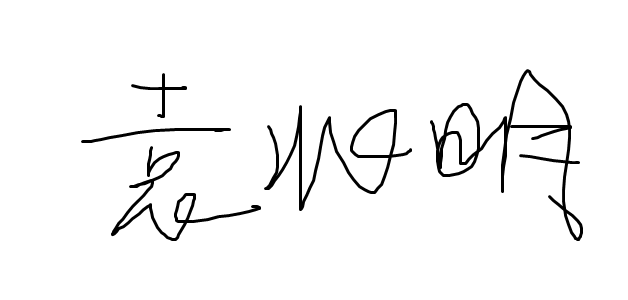
\includegraphics[width=0.2\textwidth]{sign.png} (Signed)

YUAN Zhaoming (Name of student)
\pagenumbering{roman}
%\chapter*{Dedication}

\bigskip
This thesis is dedicated to ...
\chapter*{Abstract}

\bigskip

Parabolic equations are essential in applications like heat conduction, diffusion processes, and financial modeling. They describe how quantities such as temperature, concentration, or option prices evolve over time, making them crucial in engineering, physics, and economics. This thesis aims to develop efficient numerical methods for solving parabolic problems, particularly in phase-field models, ensuring high accuracy while preserving maximum bound and energy decay properties.


In the first part of thesis, we consider the development and analysis of the structure preserving schemes for solving Allen--Cahn equations, that represents an important application of parabolic equations. We apply a $k$-th order single-step method in time, where the nonlinear term is linearized using multi-step extrapolation. In space, we use a lumped mass finite element method with piecewise $r$-th order polynomials and Gauss–Lobatto quadrature. At each time level, a cut-off post-processing technique is proposed to eliminate values that violate the maximum bound principle at the finite element nodal points. As a result, the numerical solution satisfies the maximum bound principle at all nodal points, and the optimal error bound $O(\tau^k + h^{r+1})$ is theoretically proven. These time-stepping schemes include algebraically stable collocation-type methods, which can achieve arbitrarily high order in both space and time. By combining the cut-off strategy with the scalar auxiliary variable (SAV) technique, we develop a class of energy-stable and maximum bound preserving schemes that are arbitrarily high-order in time.



In the second part, we present the development and analysis of a class of single-step implicit-explicit  schemes for approximately solving linear parabolic equations, which achieves long-time stability and arbitrarily high order in time. This involves splitting the linear operator into symmetric and skew-symmetric components, evaluated implicitly and explicitly, respectively, using the Implicit-Explicit Runge--Kutta Method (IMEX-RK). For the symmetric part, a diagonally implicit method (DIRK) is employed, while the discretization for skew-symmetric part is designed to satisfy the stage orders. This method is applicable to semilinear problems, such as phase-field models, and our analysis is consistent with existing findings, showing energy stability for certain IMEX-RK schemes. Our results reveal intersections up to at least third order, leading to a scheme that preserves both the original energy decay properties and maximum bound principles. 


In the third part of the thesis, we study the parareal algorithm for solving parabolic equations,which enables parallel-in-time computation and significantly accelerates the process. We prove that the parareal method has a robust convergence rate of about 0.3, provided the ratio $J$ of coarse to fine step size exceeds a certain threshold $J_*$, and the fine propagator meets mild conditions. This convergence is robust even with nonsmooth problem data and boundary condition incompatibilities. Qualified methods include all absolutely stable single-step methods with a stability function satisfying $|r(-\infty)| < 1$, allowing the fine propagator to be of arbitrarily high order. Moreover, we examine popular high-order single-step methods, such as the two-, three-, and four-stage Lobatto IIIC methods, confirming that their corresponding parareal algorithms converge linearly with a factor of $0.31$, with a threshold $J_* = 2$. 

At the end of each chapter, we present numerical results that support the theoretical findings and inspire future investigations.
%\chapter*{Publications arising from the thesis}

\bigskip

\begin{refsection}
\nocite{Cutoff2022,parareal2022}

\printbibliography[heading = none]
\end{refsection}
\chapter*{Acknowledgements}

\bigskip


In this part, I would like to share my appreciate to 
some people or some organisations that might contribute 
to the thesis and my study. 

I was born in a northern city of China, named Qiqihar, 
in which the snow covers everything about six months 
each year. That was tough days for me but thanks to 
a series of people from my relatives, the communities 
and the schools, I could enter Beijing Normal University. 

I start the first calculus in middle school, and 
I would call that the start of my mathematical career. 
I visited every famous bookstore in Qiqihar, and collected 
the books there, since the e-books were less popular and 
I cannot get them. 
Although I have to admit that the books there were bad, 
they inspired me, and later I started majoring mathematics 
till now. 

People say that Gaokao is important in China, but I did not 
take it a big deal. It was not hard for me to enter BNU. 
Not surprisingly, based on my background, I guess I dare to 
say that I was some kind of outstanding and I honored many 
awards and scholarships. During that days, I also learnt 
a lot on many aspects of mathematics. 

The professors in BNU are very kind and responsible. 
Maybe it is because BNU is Teacher's University that 
almost all of the professors are good and talent in 
teaching, but that is definitely not the only reason. 
Some professor will support a discuss session and audit it, 
and the students would collect the questions, and present 
them. I learnt LaTeX during the prediscussion, Prof. Liu 
helped us on the typing and formatting the documents 
on his spare time. I would also thank other teachers and 
professors, Prof. Huang, Dr. Liu, Eng. Liu, Dr. Wang, etc. 
who taught me or helped me. 
I also learnt a series of softwares or platforms 
during that days, and some of them I am still using 
in my research and in my thesis. 

I met my current supervisor in BNU. Late Professor Zhang 
introduced me to Dr. Zhou, and we discussed about the research plan. Dr. Zhou allowed me to present his Research Assistant and then Dr. Yang and Dr. Zhou offered and funded me their collaborate Ph.D. programme. 
Dr. Zhou also encouraged me on the preparation and application. They have my deep thanks. 

In the days in Hong Kong, from ruins and pandemic we suffered, remotely the studying and researching we did. 
Everyone, supervisors, professors, instructors, classmates, 
and friends from chatgroups or internets, supported me
and supported each other during that days. 
I also finished some papers and researches that days. 
I would also appreciate the help from my supervisor, 
Dr. Zhou and Dr. Yang on my research, including topics, advising, discussions, answering my questions, 
and helping me on my papers.  
I would also thank Dr. Zhang, Dr. Wang, Mr. Li and other teachers and collaborators for the helping and discussion with my research.

I will finish my postgraduate study after the thesis. 
The new occupation is ready and offered. 
Many rejection has been received and finally I get 
the right one. I would like to thank Dr. Zhou, 
Dr. Yang, Dr. Chen, Dr. Fan on my new work. 

At the end of this part, I would like to thank my girlfriend, my love and my wife-to-be, Dr. Fan Ganghua. 
We met at BNU, and will get married soon. Since then, 
we have been through everything together. 
She is the first and the last one who encouraged me on everything, on postgraduate application, 
on tough days, on research and on my occupation. 
I can hardly finish all of these on myself without her help.

%Some people that may contributed to this thesis: Dr. Kai WANG(Central South University, China), Dr. Jiang YANG (Southern University of Science and Technology), Dr. Zhi ZHOU (The Hong Kong Polytechnic University). 

%Softwares or platforms that may contributed to this thesis:  C/C++, CUDA, Dropbox, Eigen, FreeFEM, GNU-Compiler(gcc), MATLAB, numpy, OneDrive, OpenMP, OutLook, Overleaf,  Python, QQ, TencentMeeting, TeXLive, VSCode, WeChat, Zoom. 

%Funding that may related to my thesis: todo. 


\tableofcontents
%\listoffigures
%\listoftables

\pagenumbering{arabic}



\chapter{Introduction}




\section{Research Background}

Parabolic differential equations are essential in various scientific fields, including physics, engineering, and economics. In physics, they are used to describe heat conduction, diffusion processes, and the behavior of semiconductors. In finance, they are used in the Black-Scholes model for option pricing. In biology, they are used to model population dynamics and the spread of diseases.
Additionally, the study of parabolic differential equations has introduced many important mathematical concepts and techniques. The method of separation of variables, commonly used to solve these equations, is a fundamental tool in mathematical analysis. The theory also plays a crucial role in studying stochastic processes and Brownian motion.
Parabolic differential equations remain a central topic in mathematical analysis and applied mathematics. They have a rich history and are still an active area of research, offering many challenging problems and applications.

Phase field models are one of the most important applications of parabolic equations, which are mathematical tools widely used in physics, materials science, and other fields to describe the evolution of complex microstructures. They are particularly useful for modeling phase transitions, such as the solidification of a liquid or the formation of crystals in a solution.

Introduced in the late 20th century, the phase field approach addresses challenges associated with traditional methods for modeling phase transitions. Traditional methods often involve sharp interfaces between different phases, which can be difficult to handle both mathematically and computationally. In contrast, the phase field approach treats interfaces as diffuse regions and describes the microstructure using a continuous field variable, simplifying the mathematical and computational processes. Phase field models have been applied to a wide range of phenomena, including crystal growth, grain boundary motion, and pattern formation in alloys. They are also used in areas such as fluid dynamics, image processing, and tumor growth modeling.

In a phase field model, the microstructure is represented by a phase field variable that varies continuously between phases. The evolution of this phase field is governed by parabolic equations derived from thermodynamic and kinetic principles. These equations are solved numerically using various computational methods.


Structure-preserving schemes are numerical methods used in computational mathematics and physics. They are designed to maintain the inherent geometric or physical properties of the problem being solved. Structure preservation is crucial in many scientific and engineering applications, such as molecular dynamics, fluid dynamics, and electromagnetism, where preserving properties like energy, momentum, or symplectic structure is essential for the physical relevance and accuracy of the solution. These schemes often provide more accurate and physically relevant solutions than traditional numerical methods, especially in long-term simulations and highly nonlinear problems. 

For phase field models, researchers focus on developing numerical schemes that preserve \textbf{energy dissipation law} and \textbf{maximum bound principle}, without strict constraints on time step and space mesh sizes. For example, we focus on the development and analysis of high-order structure-preserving schemes for solving the Allen--Cahn equation:
\begin{equation}\label{eqn:AC}
    \begin{cases}
    u_t = \Delta u + f(u) &
        \mbox{in~~} \Omega\times(0,T),\\
    u(x,t=0) = u_0(x)   &
        \mbox{in~~} \Omega\times\{0\},\\
    \partial_{\mathbf{n}}u = 0  &
        \mbox{on~~} \partial\Omega\times(0,T)
  \end{cases}
\end{equation}
where $\Omega$ is a smooth domain in $\mathbb{R}^d$ with the boundary $\partial\Omega$. Here, $f(u)=-F'(u)$ with a double-well potential $F$ that has two wells at $\pm\alpha$, for some known parameter $\alpha>0$.
It is well-known that the Allen--Cahn equation \eqref{eqn:AC} has the \textbf{maximum bound principle} \cite{DuJuLiQiao:2020}:
\begin{align}\label{eqn:max-AC}
|u_0(x)|\le \alpha\quad{\Rightarrow}\quad |u(x,t)| \le \alpha\qquad \text{for all} ~~(x,t)\in \Omega\times(0,T].
\end{align}
As a typical $L^2$ gradient flow associated with the following free energy:
$$E(u)=\int_\Omega\frac{1}{2}|\nabla u|^2+F(u)\,\mathrm{d}x,$$
the nonlinear \textbf{energy dissipation law} holds:
\begin{equation}\label{enlaw}
\frac{\d}{\d t}E(u)=-\int_\Omega|u_t|^2\,\mathrm{d}x\le 0.
\end{equation}

We aim to develop high-order numerical schemes that preserve both conditions \eqref{eqn:max-AC} and \eqref{enlaw}. Additionally, we will discuss efficient parallel-in-time algorithms for solving the (nonlinear) parabolic equations.

\section{Literature Review} 

In this part, we briefly review the existing literature on structure-preserving schemes for solving parabolic equations and phase-filed models.

The backward Euler time-stepping scheme, combined with the central finite difference method in space, effectively preserves the maximum principle for linear parabolic equations \cite[Chapter 9]{Larsson-Thomee-2003}. Additionally, using the backward Euler scheme with the lumped mass linear finite element method (FEM) and simplicial triangulation with acute angles also maintains this principle. In two dimensions, this extends to Delaunay-type triangulations, which is notably sharp \cite{Thomee:2008}. However, without mass lumping, standard Galerkin FEMs generally do not preserve the maximum principle \cite{Thomee:2008, Schatz:2010}. These methods achieve first-order accuracy in time and second-order accuracy in space.

The development and analysis of maximum bound preserving schemes for Allen--Cahn equations have been intensively studied in existing references.
It was proved in \cite{tangyang1,ShenTangYang:2016} that the stabilized semi-implicit Euler time-stepping scheme,
with central difference method in space, preserves the maximum principle unconditionally
if the stabilizer satisfies certain restrictions. In \cite{DuJuLiQiao:2019},
a stabilized exponential time differencing scheme was proposed for solving the (nonlocal) Allen--Cahn equation,
and the scheme was proved to be unconditionally MBP. See also \cite{DuJuLiQiao:2020}
for the generalization to a class of semilinear parabolic equations.

The development and analysis of maximum bound preserving schemes for Allen--Cahn equations have been intensively studied in existing references.
It was proved in \cite{tangyang1,ShenTangYang:2016} that the stabilized semi-implicit Euler time-stepping scheme,
with central difference method in space, preserves the maximum principle unconditionally
if the stabilizer satisfies certain restrictions. In \cite{DuJuLiQiao:2019},
a stabilized exponential time differencing scheme was proposed for solving the (nonlocal) Allen--Cahn equation,
and the scheme was proved to be unconditionally MBP. See also \cite{DuJuLiQiao:2020}
for the generalization to a class of semilinear parabolic equations.

%\mycomment{Move To Next Ch.?}
High-order strong stability preserving (SSP) time-stepping methods are widely used
in the development of MBP scheme for both parabolic equations and hyperbolic equations (see e.g.,  
\cite{gottlieb1998total,Liu-Yu-2014,GottliebShuTadmor:2001,gottlieb2011strong,Liu-Osher-1996,Qiu-Shu-2005,Xu-2014,Zhang-Shu-2010}).
Recently, an SSP integrating factor Runge--Kutta method of up to order four was proposed and
analyzed in \cite{IsherwoodGrantGottlieb:2018} for semilinear hyperbolic and parabolic equations.
For semilinear hyperbolic and parabolic equations with strong stability (possibly in the maximum norm), the method
can preserve this property and can avoid the standard parabolic CFL condition $\tau=O(h^2)$, only requiring
the stepsize $\tau$ to be smaller than some constant depending on the nonlinear source term, also referring to \cite{ju2020maximum}.
A nonlinear constraint limiter was introduced in \cite{Vegt-Xia-Xu-2019} for implicit time-stepping
schemes without requiring CFL conditions, which can preserve maximum principle at the
discrete level with arbitrarily high-order methods by solving a nonlinearly implicit system.

Very recently, a new class of high-order MBP methods was proposed in \cite{LiYangZhou:sisc}.
The method consists of a $k$th-order multistep exponential integrator
in time, and a lumped mass finite element method in space with piecewise $r$th-order
polynomials. At every time level, the extra values exceeding the maximum bound
are eliminated at the finite element nodal points by a cut-off operation.
Then the numerical solution at all nodal points
satisfies the MBP, and an error bound of $O(\tau^k + h^r)$ was proved. However, numerical results in \cite[Table 4.1]{LiYangZhou:sisc}
indicates that the error bound is not sharp in space, and how to improve the estimate it is still open.
%As far as we know, this is the first work presenting arbitrarily high-order unconditionally MBP schemes with provable error estimates.
Besides, the aforementioned scheme requires to evaluate some actions of exponential functions of diffusion operators,
which might be relatively expensive compared with solving poisson problems, and the generalization to other time stepping schemes is a nontrivial task.
Finally, the proposed scheme (with relatively coarse step sizes) might produce a numerical solution with obviously
increasing and oscillating energy. These motivate our current project.

There have been numerous studies focused on developing various numerical schemes that preserve the energy dissipation law at a discrete level. Some notable and widely-used implicit time-stepping methods include convex splitting methods \cite{gradsys, epitaxy3} and the Crank-Nicolson type scheme \cite{MR4242247, CHCN1}. The main drawback of these methods is the high computational cost associated with solving a nonlinear system of equations at each time step. In contrast, implicit-explicit (IMEX; also known as semi-implicit) methods handle the nonlinear term explicitly and the linear term implicitly, requiring only the solution of a linear system of equations at each time step. These methods can be traced back to the work of Chen and Shen \cite{IMEXpf1} in the context of phase-field models, and since then, many techniques and strategies have been developed to design such schemes, as seen in \cite{akrivis2019energy, Wangxm, yang2015SDC, splitting1, xuyan, opspltLi, shen2019new, ACCH, ATA}. Building on the concept of the invariant energy quadratization (IEQ) method \cite{IEQ1, IEQ2}. \cite{ShenXu:2018, shen2019new} proposed the scalar auxiliary variable (SAV) method, which easily ensures the unconditional energy decay property. Recently, some modified SAV methods have been developed \cite{SAVcheng, SAVxu, SAVqiao, TWY-JSC22}. However, the energy considered in these methods is modified from the original energy. In another direction, exponential time differencing (ETD) methods for the Allen–Cahn equation and other semilinear parabolic equations have garnered significant attention recently. Du et al. \cite{DuJuLiQiao:2019} demonstrated that ETD and ETDRK2 schemes unconditionally preserve the maximum bound property (MBP) and energy stability (though not the dissipation law). Specifically, \cite{fuyangetd} establishes the original energy stability for ETDRK2. For the thin film model (or MBE model), interesting results regarding stability analysis and error estimates for the ETD schemes are presented in \cite{ETDstiff, ETDanal, ju2018energy, epxywithornot, epitaxy4}. Additionally, \cite{fimRk} shows that fully implicit Runge-Kutta (RK) methods can reduce the energy of gradient systems, but the existence and uniqueness of the solution remain unresolved issues. Another class of implicit Runge-Kutta methods for phase-field models is based on the convex splitting approach, which exhibits favorable stability properties \cite{convexsplitphasefield}.

Time-stepping schemes for solving parabolic equations traditionally require sequential computation, which can be time-consuming. However, with modern computing power, parallel-in-time (PinT) methods have become feasible, allowing simultaneous computation of multiple time steps. Originating from Nievergelt's work in 1964 \cite{Nievergelt:1964}, these methods have gained considerable interest. Among them, the parareal method, introduced in 2001 \cite{LionsMadayTurinici:2001}, is particularly popular due to its simplicity and adaptability with single-step integrators. It has been effectively applied in various fields such as turbulent plasma \cite{Reynolds-Barredo:2012, Reynolds-Barredo:2013}, structural dynamics \cite{CortialFarhat:2009, Farhat:2003}, molecular dynamics \cite{Baffico:2002}, optimal control \cite{MadaySalomonTurinici:2007, MathewSarkisSchaerer:2010}, and fractional models \cite{LiTangXu:2013, WuZhou:2017frac}. For more comprehensive insights, readers can consult survey papers \cite{Gander:2015, OngSchroder:2020} and references therein.


\section{Our Contribution}
In this thesis, we discuss the development, analysis, and implementation of structure-preserving single-step integrators for solving parabolic equations, with applications to phase-field models like the Allen-–Cahn equations. Single-step integrators often offer better stability properties than linear multistep methods, particularly for stiff problems, allowing for larger time steps and more efficient simulations. Additionally, they provide superior error control, especially when using adaptive time steps. Compared to linear multistep methods, single-step integrators are also more suitable for applying postprocessing techniques to preserve certain structures, as we will explore in this thesis.


In the first part of thesis, we develop and analyze a class of maximum bound preserving schemes for approximately solving Allen--Cahn equations.
We apply a $k$th-order single-step scheme in time (where the nonlinear term is linearized by multi-step extrapolation),
and  a lumped mass finite element method in space with piecewise
$r$th-order polynomials and Gauss--Lobatto quadrature. At each time level, a cut-off post-processing
is proposed to eliminate extra values violating the maximum bound principle at the finite element nodal points.
As a result, the numerical solution satisfies the maximum bound principle (at all nodal points),
and the optimal error bound $O(\tau^k+h^{r+1})$ is theoretically proved for a certain class of schemes. The proof is based on energy estimation. Since cut-off itself will not increase the total energy, we just compare each step with its previous step, which is decoupled with postprocessing and complete the proof.
These time stepping schemes under consideration includes algebraically stable collocation-type methods,
which could be arbitrarily high-order in both space and time. 
Moreover, combining the cut-off strategy with the scalar auxiliary value (SAV) technique,
we also develop a class of energy-stable and maximum bound preserving schemes, which is arbitrarily high-order in time. 



In the second part of this thesis, we explore implicit-explicit Runge--Kutta methods for solving parabolic equations. We begin by examining linear parabolic problems where the differential operator may be non-selfadjoint, which is crucial in applications like Stokes--Darcy coupled systems \cite{HanspalWaghodeNassehiWakeman:2006,Nassehi:1998,ArbogastGomez:2009}. These systems are often used to model contaminant transport in karst aquifers, where fluid motion in porous media is coupled with conduits. During floods, contaminants can enter the porous media and be released during droughts. Accurate numerical schemes are essential for capturing the long-term retention and release of contaminants, as fluid motion in porous media is slower than in conduits.

To address this, we develop a class of implicit-explicit Runge--Kutta methods and prove their long-term stability and error estimates. We split the differential operator into symmetric and skew-symmetric parts: the skew-symmetric part and source term are evaluated explicitly, while the symmetric part is evaluated implicitly. Our analysis uses spectral decomposition of the symmetric operator and energy estimation. We establish a novel energy argument to demonstrate long-term stability and optimal error estimates, choosing a special test function inspired by the backward Euler scheme.

This approach can be extended to nonlinear phase-field models. With cutoff postprocessing at each step, we show that the method preserves the maximum bound and can achieve arbitrarily high order. In \cite{fu2024energy}, it was proven that IMEX-RK schemes can maintain energy dissipation laws under certain assumptions. Our assumptions align with theirs, and we have found a third-order scheme that meets all criteria, allowing us to develop time-stepping schemes up to third order that preserve both the maximum bound and original energy dissipation.
 

In the third part of thesis, we investigate the parareal algorithm for solving parabolic equations, which enables parallel-in-time computation and significantly accelerates the process. For linear problems, we analyzed the robust convergence of a class of parareal algorithms. 
The coarse propagator is fixed to the backward Euler method 
and the fine propagator is a high-order single step integrator. 
Under some conditions on the fine propagator, 
we show that there exists some critical $J_*$ such that t
he parareal solver converges linearly with a convergence 
rate near $0.3$, provided that the ratio between the coarse 
time step and fine time step named $J$ satisfies $J \ge J_*$. 
The convergence is robust even if the problem data is nonsmooth and incompatible with boundary conditions. 
The qualified methods include all absolutely stable single 
step methods, whose stability function satisfies 
$|r(-\infty)|<1$, and hence the fine propagator could be 
arbitrarily high-order. Moreover, we examine some popular 
high-order single step methods, e.g., two-, three- and 
four-stage Lobatto IIIC methods, and verify that the 
corresponding parareal algorithms converge linearly with a 
factor $0.31$ and the threshold for these cases is $J_* = 2$. 



 
%\section{Problem Setting}

%In this thesis, we are focusing on the following equation, 
%\begin{equation}\label{eq:parabolic}
%    u_t = \calA u + f,
%\end{equation}
%together with initial and boundary value conditions, 
%where $u:\Omega\times I   \to \bbR$ is a variable. 
%$\Omega \subset \bbR^d$ is the space domain, 
%$d$ is the dimension on space. 
%$I \subset \bbR$ is the time interval. 
%$\calA$ is a differential operator, maybe linear or nonlinear. 
%For simplicity reasons, we fix $I = (0, T)$ throughout the thesis. 


%\subsection{Allen-Cahn Equation}

%We will design and analyze a high-order maximum bound preserving (MBP) scheme for solving the Allen--Cahn equation:
%\begin{equation}\label{eqn:AC}
%    \begin{cases}
%    u_t = \Delta u + f(u) &
 %       \mbox{in~~} \Omega\times(0,T),\\
 %   u(x,t=0) = u_0(x)   &
%        \mbox{in~~} \Omega\times\{0\},\\
%    \partial_{\mathbf{n}}u = 0  &
 %       \mbox{on~~} \partial\Omega\times(0,T)\\
%  \end{cases}
%\end{equation}
%where $\Omega$ is a smooth domain in $\mathbb{R}^d$ with the boundary $\partial\Omega$.
%$f(u)=-F'(u)$ with a double-well potential $F$ that has two wells at $\pm\alpha$, for {some known parameter $\alpha>0$}. %; see Examples \ref{AC:1} and \ref{AC:2}
%For two popular choices of potentials. It is well-known that the Allen--Cahn equation \eqref{eqn:AC} has the maximum bound principle \cite{DuJuLiQiao:2020}:
%\begin{align}\label{eqn:max-AC}
%|u_0(x)|\le \alpha\quad \Longrightarrow\quad |u(x,t)| \le \alpha\qquad \text{for all} ~~(x,t)\in \Omega\times(0,T].
%\end{align}
%As a typical $L^2$ gradient flow associating with the following free energy
%$$E(u)=\int_\Omega\frac{1}{2}|\nabla u|+F(u)\d x,$$
% the nonlinear energy dissipation law holds in the sense
%\begin{equation}\label{enlaw}\frac{\d}{\d t}E(u)=-\int_\Omega|u_t|^2\d x\le 0.\end{equation}
 

% \section{Single-Step Method}

% To solve equation \eqref{eq:parabolic}, 
% we split the interval $(0,T)$ into $N$ subintervals with the uniform mesh size $\tau=T/N$,
% and set $t^n = n\tau$, $n=0,1,\ldots,N$. 
% Define $u^n: \Omega \to \bbR$ as an approximation of $u(t^n)$, 
% and $E(\tau)$ is the solution operator,
% the general form of single-step method can be shown as 
% \begin{equation}\label{eq:single-step}
%     u^n = E(\tau) (u^{n-1}), \quad \text{if}~n \geq 1
% \end{equation}
% \subsection{Postprocessing}

% Postprocessings are widely used in the numerical simulations, especially single-step methods, 
% that that we would furtherly modify the result after each time level. 
% This is often because the direct result of numerical simulation 
% is less acceptable for some specific criteria and should be repaired, 
% such that it failed on energy decay property, failed on maximum bound preserving, 
% or failed on mass conservation law, and may cause unstable or singularity. 

% In this thesis, it is cut-off that we will mainly use on our approximation. 
% There are some direct reason that we should perform cut-off postprocsessing:
% \begin{itemize}
%     \item[1.] maximum bound preserving; 
%     \item[2.] singularity of the potential term; 
%     \item[3.] Lipschitz continuity. 
% \end{itemize}





% \section{Runge--Kutta Method}

% Consider $f = f(t^n)$ is a time-dependent source term for linear inhomogeneous equation. 
% Runge-Kutta method is a widely used numerical technique for solving ordinary differential equations (ODEs). It is an iterative method that provides an approximate solution to the ODEs by discretizing the problem into smaller subintervals and using a set of formulas to update the solution at each step.

% The Runge-Kutta methods come in different orders of accuracy, 
% with the most famous ones being the 4th order Runge-Kutta method 
% (RK4) and the 2nd order Runge-Kutta method (RK2), 
% based on the approximations to related internal points (called stages). 
% Here we will use Implicit Runge--Kutta Methods (Implicit RK) and Implicit-Explicit Runge--Kutta Methods (IMEX-RK) in this work. 

% The $m$-stage Implicit RK methods reads as 
% % In particular, at level $n$, with given $u_h^{n-k},\ldots, u_h^{n-1}\in S_h^r$, we find an intermediate solution $\hat u_h^{n}\in S_h^r$ such that
% \begin{equation}\label{eq:RK-implicit}
%     \begin{cases}
%     u^{ni} = u^{n-1} + \tau \sum_{j=1}^m a_{ij} (\calA u^{nj} + f(t^{nj})) &\quad \text{for} ~~i=1,2,\dots,m, \\
%     u^{n} = u^{n-1} + \tau \sum_{i=1}^m b_i (\calA u^{ni} + f(t^{ni})),
%   \end{cases}
% \end{equation}
% and the $m$-stage IMEX-RK methods read as 
% \begin{equation}\label{eq:RK-implicit-explicit}
%     \begin{cases}
%     u^{ni} = u^{n-1} + \tau \sum_{j=0}^m a_{ij} \calA u^{nj} + \tau \sum_{j=0}^m \hata_{ij} f(t^{nj}) &\quad \text{for} ~~i=1,2,\dots,m, \\
%     u^{n} = u^{n-1} + \tau \sum_{i=0}^m b_i \calA u^{ni} + \tau \sum_{i=0}^m \hatb_if(t^{ni}),
%   \end{cases}
% \end{equation}

% Ususlly, these coefficients are usually arranged 
% in a mnemonic device, known as a \emph{Butcher tableau}. 
% \begin{table}[h]
%     \begin{center}
%     \begin{tabular}{lll|ll}
%     $a_{11}$  &\ldots &$a_{1m}$ &$c_1$  &  \\
%     \vdots    &       &\vdots   &\vdots &  \\
%     $a_{m1}$  &\ldots &$a_{mm}$ &$c_m$  &  \\ \cline{1-4}
%     $b_{1}$   &\ldots & $b_{m}$ & &
%     \end{tabular}
%     \end{center}
%     \caption{Butcher tableau for Implicit RK scheme.}\label{tab:RK}
%     \end{table}
%     \begin{table}[h]
%         \centering
%         \begin{tabular}[h]{c|ccccc|ccccc}
%             $0$ & $0$ & & & & & $0$ \\
%             $c_1$ & $0$& $a_{11}$ & $0$ & $\dots$ & $0$ & $\hata_{10}$ & $0$ & $\dots$ & $0$& $0$ \\
%             $c_2$ & $0$& $a_{21}$ & $a_{22}$  & $\dots$ & $0$ & $\hata_{20}$ & $\hata_{21}$ & $\dots$ & $0$ & $0$\\
%             $\vdots$ & $0$& $\vdots$ & $\vdots$  & $\ddots$ & $\vdots$ & $\vdots$ & $\vdots$ & $\ddots$ & $\vdots$ & $0$\\
%             $c_m$ & $0$& $a_{m1}$ & $a_{m2}$  & $\dots$ & $a_{mm}$ & $\hata_{m0}$ & $\hata_{m1}$ & $\dots$ & $\hata_{m,m-1}$ & $0$\\
%             \hline
%             & $0$& $b_1$ & $b_2$ & $\dots$ & $b_m$ & $\hatb_0$ & $\hatb_1$ & $\dots$ & $\hatb_{m-1}$& $0$
%         \end{tabular}
%         \caption{Butcher tableau for IMEX-RK scheme.}
%         \label{tab:Butcher}
%     \end{table}
    

% \section{Parareal Method}

% The Parareal method is a parallel numerical technique designed to efficiently solve time-dependent problems in scientific computing. It was introduced by Yves Robert and Jean-Philippe Pouchet in 2001 to tackle the challenges of long-duration simulations, particularly in fields such as molecular dynamics, quantum chemistry, and fluid dynamics.


% The Parareal algorithm is based on the idea of parallelizing the solution of a complex problem by dividing it into several smaller subproblems that can be solved independently. It leverages two types of solvers:

% {\bf Coarse Solver}: A fast but less accurate solver that provides an approximate solution to the problem over a given time interval.

% {\bf Fine Solver}: A more accurate but computationally intensive solver that yields precise solutions when high precision is required.

% In parareal method, The time domain of the problem is divided into multiple smaller intervals.
% A coarse solver is used to quickly solve each interval in parallel, starting from the initial conditions, 
% while for each interval, a fine solver recalculates the solution at the end point and corrects the coarse solver's result, providing a correction term. 
% The correction is fed back into the initial conditions of the next interval, and the process is repeated until the desired accuracy is achieved.

% The method significantly improves computational efficiency by solving multiple intervals in parallel.








\chapter{Arbitrarily High-order Maximum Bound Preserving Schemes with Cut-off Postprocessing}


In this chapter, we develop and analyze a class of maximum bound preserving schemes for approximately solving Allen--Cahn equations.
We apply a single-step scheme in time with nonlinear term linearized, and a lumped mass finite element method in space. At each time level, a cut-off post-processing
is proposed to eliminate extra values violating the maximum bound principle at the finite element nodal points.
As a result, the numerical solution satisfies the maximum bound principle (at all nodal points),
and the optimal error bound is theoretically proved for a certain class of schemes.
Moreover, combining the cut-off strategy with the scalar auxiliary value (SAV) technique,
we also develop a class of energy-stable and maximum bound preserving schemes, which is arbitrarily high-order in time.

In Section \ref{sec:2.1} we discuss the time discretization problems and show its convergence. 
In Section \ref{ssec:fully} and \ref{sec:collocation} 
we discuss the fully-discrete scheme and prove 
its convergence. In Section \ref{sec:sav} we combine our scheme with Scalar Auxiliary Variable method and 
prove it preserves modified energy decay and 
arbitrary high order in time. 

\section{Temporal Semi-discrete Cut-off Runge--Kutta Scheme}\label{sec:2.1}
To begin with, we consider the time discretization for the Allen--Cahn equation \eqref{eqn:AC}.
To this end, we split the interval $(0,T)$ into $N$ subintervals with the uniform mesh size $\tau=T/N$,
and set $t^n = n\tau$, $n=0,1,\ldots,N$.
On the time interval $[t^{n-1},t^n]$, we approximate the nonlinear term $f(u(s))$ by the extrapolation polynomial
$$
 \sum_{j=1}^{k} L_j(s) f(u^{n-j}),\quad \text{with known}~ u^{n-k},\ldots,u^{n-1}.
$$
where $L_j(s)$ is the Lagrange basis polynomials of degree $k-1$ in time, satisfying
$$
L_j(t^{n-i}) = \delta_{ij}, \quad i,j=1,\dots,k.
$$
Thus, on $[t^{n-1},t^n]$, the linearization of \eqref{eqn:AC} states as
$$\tilde{u}_t=\Delta\tilde{u}+\sum_{j=1}^{k} L_j(s) f(u^{n-j}).$$
Following Duhamel's principle yields
$$\tilde{u}(t^{n})=e^{\tau\Delta}u(t^{n-1})+\int_0^\tau e^{(\tau-s)\Delta}\sum_{j=1}^{k} L_j(t^{n-1}+s) f(u^{n-j})\d s.$$
Then a framework of a single step scheme of approximating $\tilde{u}(t^{n})$ reads:
\begin{equation}\label{eqn:semi-interpolation}
\tilde u^{n} = \sigma(-\tau\Delta) u^{n-1} + \tau \sum_{i=1}^m p_i(-\tau \Delta)
\Big(\sum_{j=1}^{k} L_j (t^{ni}) f(u^{n-j})\Big),\quad \text{for all}~n\ge k,
\end{equation}
with $t^{ni}=t^{n-1} + c_i\tau$.
Here,
$\sigma(\lambda)$ and $\{p_i(\lambda)\}^m_{i=1}$ are rational functions and $c_i$ are distinct real numbers in $[0,1]$.
For simplicity, we assume that the scheme \eqref{eqn:semi-interpolation} satisfies the following assumptions.

\begin{itemize}
\item[{\bf (P1)}] $|\sigma(\lambda)|< 1$ and $|p_i(\lambda)|\le c$, for all $i=1,\ldots,m$,
uniformly in $\tau$ and $\lambda > 0$. Besides, the numerator of $p_i(\lambda)$
is of lower degree than its denominator.
\item[{\bf (P2)}] The time stepping scheme \eqref{eqn:semi-interpolation}  is accurate of order $k$ in sense that
$$ \sigma(\lambda) = e^{-\lambda} + O(\lambda^{k+1}),\quad \text{as}~\lambda\rightarrow0. $$
and, for $0\le j\le k$
$$ \sum_{i=1}^m c_i^j p_i(\lambda) - \frac{j!}{(-\lambda)^{j+1}}\Big(e^{-\lambda}
- \sum_{\ell=0}^j \frac{(-\lambda)^\ell}{\ell!}\Big) = O(\lambda^{k-j}),\quad \text{as}~\lambda\rightarrow0. $$
\item[{\bf (P3)}] The time discretization scheme \eqref{eqn:semi-interpolation} is strictly accurate of order $q$ in sense that
$$ \sum_{i=1}^m c_i^j p_i(\lambda) - \frac{j!}{(-\lambda)^{j+1}}\Big(\sigma(\lambda)
- \sum_{\ell=0}^j \frac{(-\lambda)^\ell}{\ell!}\Big) =0,\quad\text{for all}~ 0\le j\le q-1. $$
\end{itemize}

\begin{remark}
In practice,
it is convenient to choose $p_i(\lambda)$ that share the same denominator of $\sigma(\lambda)$, for instance:
$$\sigma(\lambda) = \frac{a_0(\lambda)}{g(\lambda)},\quad \text{and} \quad p_i(\lambda) = \frac{a_i(\lambda)}{g(\lambda)},\quad \text{for}~i=1,2,\ldots,m,$$
where $a_i(\lambda)$ and $g(\lambda)$ are polynomials.
Then the time stepping scheme \eqref{eqn:semi-interpolation} could be written as
\begin{equation*}
g(-\tau\Delta)\tilde u^{n} = a_0(-\tau\Delta) u^{n-1} + \tau \sum_{i=1}^m a_i(-\tau \Delta)
\Big(\sum_{j=1}^{k} L_j (t^{ni}) f(u^{n-j})\Big),\quad \text{for all}~n\ge k.
\end{equation*}
See e.g. \cite[pp. 131]{Thomee:2006} for the construction of such rational functions satisfying the Assumptions (P1)-(P3).
\end{remark}


Unfortunately, the time stepping scheme \eqref{eqn:semi-interpolation} does not satisfy the maximum bound principle. Therefore,
at each time step, we apply the cut-off operation: for $n\ge k$, we find $u^n$ such that
\begin{align}
\hat u^{n} &= \sigma(-\tau\Delta) u^{n-1} + \tau \sum_{i=1}^m p_i(-\tau \Delta)
\Big(\sum_{j=1}^{k} L_j (t^{ni}) f(u^{n-j})\Big),\label{eqn:semi-1}\\
u^{n} &=  \min(\max(\hat u^{n},-\alpha),\alpha),\label{eqn:semi-cut}
\end{align}
where $\alpha$ is the maximum bound given in \eqref{eqn:max-AC}.
%Due to the cut-off operation \eqref{eqn:semi-cut}, the semi-discrete solution
%obtained from \eqref{eqn:semi-1}-\eqref{eqn:semi-cut} satisfies
%$$
%|u^{n}(x)|\le \alpha \quad \forall\, x\in \Omega.
%$$
The accuracy of this cut-off semi-discrete method is guaranteed by the next theorem.


\begin{theorem}\label{thm:semi}
Suppose that the Assumptions (P1) and (P2) are fulfilled, and (P3) holds for $q=k$.
Let $u(t)$ be the solution to the Allen--Cahn equation, and $u^n$ be the solution to the time stepping scheme
\eqref{eqn:semi-1}-\eqref{eqn:semi-cut}.
Assume that $|u_0|\le \alpha$ and the maximum principle \eqref{eqn:max-AC} holds,
and assume that the starting values $u^j$, $j=0,\dots,k-1$, are given and
$$
|u^j|\le \alpha, \quad \text{for all}~~j=0,\dots,k-1.
$$
Then the semi-discrete solution given by  \eqref{eqn:semi-1}-\eqref{eqn:semi-cut} satisfies for all $n\ge k$
\begin{align*}%\label{eqn:semi-mbp}
|u^n|\le \alpha,
\end{align*}
and
\begin{equation*}%\label{eqn:semi-error}
\|u^n - u(t^n)\|\leq C\tau^k + C\sum_{j=0}^{k-1}\|u^j - u(t^j)\|,
\end{equation*}
provided that  $f$ is locally Lipschitz continuous, $\Delta u\in C^{k}([0,T]; L^2\II)$, $ u\in C^{k+1}([0,T];L^2\II)$ and $f(u) \in C^k([0,T];L^2\II)$.
\end{theorem}

\begin{proof}
Due to the cut-off operation \eqref{eqn:semi-cut}, the discrete
maximum bound principle follows immediately.
Then it suffices to show the error estimate.

Let $e ^n=u^n-u(t^n)$ and $\hat e ^n=\hat u^n-u(t^n)$. Since the exact solution satisfies the maximum bound \eqref{eqn:max-AC}, we have
$$  \|  e ^n  \|_{L^2\II} \le  \|  \hat e ^n  \|_{L^2\II}. $$
Then it is easy to note that
$$  \hat e^{n} = \sigma (-\tau\Delta) e ^{n-1} + \fy^n,\quad n \ge k. $$
where $\fy^n$ can be written as
\begin{align*}
  \fy^n &= -u(t^{n}) + \sigma(-\tau\Delta) u(t^{n-1}) + \tau \sum_{i=1}^m p_i(-\tau \Delta)
  \Big(\sum_{j=1}^{k} L_j (t^{ni}) f(u^{n-j})\Big) \\
  &= \tau \sum_{i=1}^m p_i(-\tau \Delta)\Big(  \sum_{j=1}^{k} L_j (t^{ni}) f(u^{n-j}) - f(t^{ni}))\Big)\\
  &\quad + \Big(-u(t^{n}) + \sigma(-\tau\Delta) u(t^{n-1}) + \tau \sum_{i=1}^m p_i(-\tau \Delta) (\partial_t u - \Delta u) (t^{ni})\Big)\\
  &=: I + II.
\end{align*}
Then the bound of $I$ follows  from the approximation property of Lagrange interpolation, the maximum bound of $u^{n-j}$ and $u(t^{n-j})$, $j=1,\ldots,k$,
the locally Lipschitz continuity of $f$, and the Assumption (P1):
\begin{align*}
   \|  I  \|_{L^2\II} &\le  \tau \sum_{i=1}^m \| p_i(-\tau \Delta)\|_{L^2\II\rightarrow L^2\II} \Big\|\sum_{j=1}^k L_j(t^{ni}) f(u(t^{n-j}))- f(u(t^{n-1} + c_i\tau))\Big\|_{L^2\II}\\
   &\qquad + \tau \sum_{i=1}^m \| p_i(-\tau \Delta)\|_{L^2\II\rightarrow L^2\II} \sum_{j=1}^k |L_j(t^{ni})|\,\| f(u^{n-j})- f(u(t^{n-j} ))\|_{L^2\II}\\
   &\le C\tau^{k+1} \|  f(u) \|_{C^{k}([t^{n-k},t^n];L^2\II)} + C \tau \sum_{j=1}^k \|  e^{n-j}  \|_{L^2\II}.
\end{align*}
Now we term to the second term $II$, which can be rewritten by Taylor's expansion at $t^{n-1}$
\begin{align*}
 II &= -\sum_{j=0}^k\frac{\tau^j}{j!} u^{(j)} (t^{n-1}) + \sigma(-\tau \Delta)u(t^{n-1})\\
  &\quad + \tau \sum_{i=1}^m p_i(-\tau \Delta) \sum_{j=0}^{k-1}
  \frac{(c_i\tau)^j}{j!}
  (u^{(j+1)} - \Delta u^{(j)})
  (t^{n-1}) + R_1 + R_2.
\end{align*}
where the remainders $R_1$ and $R_2$ are
\begin{align*}
 R_1 &= \int_{t^{n-1}}^{t^n} \frac{(t^n-s)^k}{k!} u^{(k+1)}(s) \,\d s\quad \text{and}\quad \\
  R_2 &=   \tau \sum_{i=1}^m p_i(-\tau \Delta) \int_{t^{n-1}}^{t^{n-1}+c_i\tau} \frac{(t^{n-1}+c_i\tau-s)^{k-1}}{(k-1)!} (u^{(k+1)}-\Delta u^{(k)})(s) \,\d s
\end{align*}
respectively. Hereafter, we use $u^{(j)}$ to denote the $j$th derivative in time. Then Assumption (P1) implies
\begin{align*}
 \|R_1+R_2\|_{L^2\II} &\le C \tau^{k+1} \Big(\|  u \|_{C^{k+1} ([t^{n-1},t^n];L^2\II)} + \|  \Delta u \|_{C^{k} ([t^{n-1},t^n];L^2\II)} \Big).
\end{align*}
Now we revisit the three leading terms of $II$. Note that
\begin{align*}
& -\sum_{j=0}^k\frac{\tau^j}{j!} u^{(j)} (t^{n-1}) + \sigma(-\tau \Delta)u(t^{n-1})
  + \tau \sum_{i=1}^m p_i(-\tau \Delta) \sum_{j=0}^{k-1} \frac{(c_i\tau)^j}{j!}
  (u^{(j+1)} - \Delta u^{(j)})(t^{n-1})\\
 =& \Big(-I +  \sigma(-\tau \Delta) - \tau \sum_{i=1}^m p_i(-\tau \Delta) \Delta \Big)u(t^{n-1}) \\
 & +   \sum_{j=1}^{k-1} \frac{\tau^j}{j!} \Big(- I  +  j \sum_{i=1}^m c_i^{j-1} p_i(-\tau \Delta) - \tau\sum_{i=1}^m c_i^{j} p_i(-\tau \Delta) \Delta\Big)u^{(j)}(t^{n-1})   \\
 & +  \frac{\tau^k}{k!} \Big(-I +  k\sum_{i=1}^m c_i^{k-1}p_i(-\tau\Delta)\Big )u^{(k)}(t^{n-1}) =\sum_{\ell=1}^3 II_\ell.
\end{align*}
Since the time stepping scheme is strictly accurate of order $q=k$ (by Assumption (P3)),
we have $ II_1=  II_2=0$. Meanwhile,
we apply Assumption (P3) again to arrive at for $\lambda>0$
\begin{align*}
  -1 + k \sum_{i=1}^m c_i^{k-1} p_i(\lambda) = \lambda \frac{k!}{(-\lambda)^{k+1}} \Big(\sigma(\lambda)-\sum_{\ell=0}^k\frac{(-\lambda)^\ell}{\ell!}\Big) =: \lambda \gamma(\lambda).
\end{align*}
Note that $|\gamma(\lambda)|=O(1)$ for $\lambda\rightarrow0$ (by Assumption (P2))
and $|\gamma(\lambda)|\rightarrow 0$ for  $\lambda\rightarrow +\infty$. Hence $|\gamma(\lambda)|$ is bounded
uniformly in $[0,\infty)$. Then we arrive at
\begin{align*}
\|  II_3 \|_{L^2\II} \le C \tau^{k+1} \|  \Delta u^{(k)}(t^{n-1}) \| \le  C \tau^{k+1} \|  \Delta u \|_{C^{k}([t^{n-1},t^n];L^2\II)}.
\end{align*}
In conclusion, we obtain the following estimate
\begin{align*}
\|  e ^n \|_{L^2\II} \le \|  \sigma(-\tau \Delta)e ^{n-1} \|_{L^2\II}  +  C \tau^{k+1}  + C \tau \sum_{j=1}^k \|  e^{n-j}  \|_{L^2\II}.
\end{align*}
Then the assumption (P1) leads to
\begin{align*}
\|  e ^n \|_{L^2\II} \le \|  e_h^{n-1} \|_{L^2\II}  +  C \tau^{k+1}  + C \tau \sum_{j=1}^k \|  e^{n-j}  \|_{L^2\II}.
\end{align*}
%and hence we rearrange terms and obtain
%\begin{align*}
%\frac{\|  e^n \|_{L^2\II} -  \|  e_h^{n-1} \|_{L^2\II} }{\tau} \le  C \tau^{k}  + C  \sum_{j=1}^k \|  e^{n-j}  \|_{L^2\II}.
%\end{align*}
Finally, the desired assertion follows immediately by using discrete Gronwall's inequality
\begin{align*}
\|  e ^n \|_{L^2\II}  \le  C e^{cT} \tau^{k}  + C e^{cT}  \sum_{j=0}^{k-1} \|  e^{j}  \|_{L^2\II}.
\end{align*}
\end{proof}

% {\color{red}
% In fact, in condition that the real solution is sufficiently smooth on space, we do not need high order strict accuracy. Assumption (P2) yields that
% $$ \sum_{i=1}^m c_i^j p_i(\lambda) - \frac{j!}{(-\lambda)^{j+1}}\Big(\sigma(\lambda)
% - \sum_{\ell=0}^j \frac{(-\lambda)^\ell}{\ell!}\Big) =O(\lambda^{k-j}),\quad\text{for all}~ 0\le j\le k-1, \lambda\rightarrow0. $$
% Assume that now we have strictly accurate of orde $k_s<k$. Therefore
% $$- 1  +  j \sum_{i=1}^m c_i^{j-1} p_i(\lambda)
% +\lambda\sum_{i=1}^m c_i^{j} p_i(\lambda)=
% \begin{cases}
%     0, &\mbox{~if~} j\leq k_s-1 \\
%     O(\lambda^{k-j+1}) \mbox{~as~} \lambda\rightarrow0, &\mbox{~if~} k_s\leq j\leq k-1,
% \end{cases}$$
% and
% $$-1 + k \sum_{i=1}^m c_i^{k-1} p_i(\lambda) = O(\lambda)
% \mbox{~as~} \lambda\rightarrow0.
% $$
% Since they tend to $0$ when $\lambda\rightarrow+\infty$, we know that they are bounded. Therefore
% \begin{align*}
%     \|  II_2 \|_{L^2\II} \le C \tau^{k+1} \sum_{j=1}^{k-k_s}\|  \Delta^{j+1} u^{(k)}(t^{n-1}) \| \le  C \tau^{k+1} \sum_{j=1}^{k-k_s}\|  \Delta^{j+1} u \|_{C^{k}([t^{n-1},t^n];L^2\II)},
% \end{align*}
%     and
% \begin{align*}
%         \|  II_3 \|_{L^2\II} \le C \tau^{k+1} \|  \Delta u^{(k)}(t^{n-1}) \| \le  C \tau^{k+1} \|  \Delta u \|_{C^{k}([t^{n-1},t^n];L^2\II)}.
% \end{align*}
% }

\begin{remark}\label{remark:p3}
Theorem \ref{thm:semi} implies that the cut-off operation preserves the maximum bound
without losing global accuracy. However, the Assumption (P3) is restrictive. It is well-known that a single step method
with a given $m \in \mathbb{Z}^+$ could be accurate of order $2m$ (Gauss--Legendre method) \cite[Section 2.2]{Ehle:thesis},
but at most strictly accurate of order $m+1$ \cite[Lemma 5]{BrennerCrouzeixThomee:1982}.
In general, a collocation-type method is only strictly accurate of order $m+1$.

Without the assumption of strict accuracy,  one may still show the error estimate,
provided that $f(u)$ satisfies certain compatibility conditions, e.g.,
$$ f(u) \in C^{\ell}([0,T]; \text{Dom}(\Delta^{k-\ell}))\quad \text{for all} \quad \ell=1,2,\ldots,k,$$
that requires
 $\partial_{\bf n} \Delta^q f(u) = 0$ for $\ell=1,2,\ldots,k-1$.
Unfortunately, those compatibility conditions cannot be fulfilled in general for semilinear parabolic problems.
%The strict accuracy is applied here to avoid those artificial compatibility conditions.
\end{remark}

\begin{remark}\label{remark:p3-2}
The same error estimate could be proved by
assuming that the scheme satisfies the assumption (P3)
with $q=k-1$ and some additional conditions
(see e.g. \cite[Theorem 8.4]{Thomee:2006} and \cite{OstermannRoche:1992}).
However, the proof is not directly applicable when we apply the cut-off operation at each time step.
It warrants further investigation to show the sharp convergence rate $O(\tau^k)$ with weaker assumptions.
\end{remark}



\section{Fully-discrete Cut-off Runge--Kutta Scheme}\label{ssec:fully}
In this part, we discuss the fully discrete scheme. To illustrate the
main idea, we consider the one-dimensional case $\Omega=[a,b]$,
and the argument could be straightforwardly extended to multi-dimensional cases, see Remark \ref{rem:highdimension}.
%The extension to multi-dimensional cases is presented in subsection \ref{section:exp-LM-mD}.
We denote by $a=x_0<x_{1}<\dots<x_{Mr}=b$ a partition of the domain with a uniform mesh size $h=x_{ir} - x_{(i-1)r} = (b-a)/M$,
and denote by $S_h^r$ the finite element space of degree $r\ge 1$, i.e.,
$$
S_h^r=\{v\in H^1(\Omega): v|_{I_i}\in P_r,\,\,\, i=1,\dots,M\} ,
$$
where $I_i=[x_{(i-1)r},x_{ir}]$ and $P_r$ denotes the space of polynomials of degree $\le r$.

Let $x_{(i-1)r+j}$ and { $\omega _{j}$}, $j=0,\dots,r$, be the quadrature
points and weights of the $(r+1)$-point Gauss--Lobatto quadrature on the subinterval $I_i$, and denote
\begin{align*}
w_{(i-1)r+j} =
\left\{
\begin{aligned}
&\omega_j &&\mbox{for}\,\,\, 1\le j\le r-1,\\
&2\omega_j &&\mbox{for}\,\,\, j=0, r.
\end{aligned}
\right.
\end{align*}
Then  we consider the piecewise Gauss--Lobatto quadrature approximation of the inner product, i.e.,
$$
(f,g)_h
:=  \sum_{j=0}^{Mr} w_j f(x_j) g(x_j)  .
$$
This discrete inner product induces a norm
$$
\|f_h\|_h=\sqrt{(f_h,f_h)_h} \quad\forall\, f_h\in S_h^r.
$$

%Note that there are $Mr+1$ quadrature points in the closed interval $[a,b]$.
%For $(Mr+1)$-dimensional vectors ${\bf u}$ and ${\bf v}$, we define the discrete $L^2$ inner product and discrete $L^2$ norm by
%$$
%({\bf u},{\bf v})_h=  {\bf M}{\bf u}\cdot {\bf v}
%\quad\mbox{and}\quad
%\|{\bf v}\|_{h}
%= \sqrt{({\bf v},{\bf v})_h} \, ,
%$$
%where ${\bf M}$ is the $(Mr+1)\times (Mr+1)$ mass matrix, a diagonal matrix consisting of the weights of the piecewise Gauss--Lobatto quadrature corresponding to the quadrature points.
Then we have the following lemma for norm equivalence. The proof follows directly from the positivity of
{Gauss--Lobatto} quadrature weights \cite[p. 426]{Quarteroni:2000}.


\begin{lemma}\label{lem:norm-equivalence}
%If $v_h\in S_h^r$ %and ${\bf v}$ is the $(Mr+1)$-dimensional vector consisting of the nodal values of $v_h$,
The discrete norm $\| \cdot \|_h$ is equivalent to usual $L^2$ norm $\| \cdot \|_{L^2\II}$ in sense that
\begin{align*}%\label{norm-equivalence}
 C_1 \|v_h\|_{L^2(\Omega)} \le \|v_h\|_h \le  C_2 \|v_h\|_{L^2(\Omega)} ,\quad \forall v_h\in S_h^r.
\end{align*}
where $C_1$ and $C_2$ are independent of $h$.
\end{lemma}

To develop the fully discrete scheme, we introduce the discrete Laplacian $-\Delta_h: S_h^r\rightarrow S_h^r$ such that
\begin{align}\label{eqn:disc-lap}
(-\Delta_h v_h, w_h)_h = (\nabla v_h, \nabla w_h)\qquad \text{for all} ~~v_h,w_h\in S_h^r.
\end{align}
Then at $n$-th time level, with given $u_h^{n-k}, \ldots, u_h^{n-1} \in S_h^r$, we find an intermediate solution
$\hat u_h^n\in S_h^r$ such that
\begin{equation}\label{eqn:fully}
 \hat u_h^n = \sigma(-\tau \Delta_h) u_h^{n-1} +\tau  \sum_{i=1}^m p_i(-\tau \Delta_h)
 \Big(\sum_{j=1}^{k} L_j (t^{ni}) \Pi_h f(u_h^{n-j})\Big)
\end{equation}
where $t^{ni}=t^{n-1}+c_i\tau$, and $\Pi_h:C(\overline\Omega)\rightarrow S_h^r$ is the Lagrange interpolation operator.
In order to impose the maximum bound, we apply the cut-off postprocessing: find $u_h^n \in S_h^r$ such that
\begin{equation}\label{eqn:fully-cut}
\begin{split}
u_h^n(x_j)  = \min\big(\max \big(\hat u_h^n(x_j), - \alpha \big) , \alpha \big),  \quad j=0,\dots,Mr.
%\Pi_h \min\big(\max \big(\hat u_h^n, - \alpha \big) , \alpha \big) .
\end{split}
\end{equation}
It is equivalent to
\begin{equation*}
u_h^n  = \Pi_h \min\big(\max \big(\hat u_h^n, - \alpha \big) , \alpha \big) .
\end{equation*}
Essentially, the cut-off operation \eqref{eqn:fully-cut} only works on the finite element nodal points.
%, and hence $u_h^n$ still belongs to $S_h^r$.


Next, we shall prove the optimal error estimate of the fully discrete scheme \eqref{eqn:fully}-\eqref{eqn:fully-cut}.
To this end, we need the following stability estimate of operators $\sigma(-\tau \Delta_h)$ and $p_i(-\tau \Delta_h) $.
\begin{lemma}\label{lem:stable-fully}
Let $\Delta_h$ be the discrete Laplacian defined in \eqref{eqn:disc-lap}, and $\sigma(\lambda)$ and $p_i(\lambda)$ are
rational functions satisfying the Assumption (P1). Then there holds that for all $v_h \in S_h^r$
\begin{equation}\label{eqn:stab-est-1}
 \|  \nabla^q \sigma(-\tau \Delta_h) v_h \|_h \le \| \nabla^q v_h \|_h
\quad \text{and}\quad \|  \nabla^q p_i(-\tau \Delta_h ) v_h \|_h \le C\| \nabla^q v_h \|_h
 \end{equation}
 with $i=1,\ldots,m$ and $q=0,1$.
 Meanwhile,
\begin{equation} \label{eqn:stab-est-2}
 \tau \|  \nabla^q \Delta_h p_i (-\tau \Delta_h) v_h \|_h   \le C \|  \nabla^q v_h \|_h
 \quad  i=1,\ldots,m, ~~q=0,1
  \end{equation}
%Here the generic constant $C$ is independent of $\tau$ and $h$.
\end{lemma}

\begin{proof}
Let $\{(\lambda_j, \fy_j^h)\}_{j=1}^{Mr+1}$ be eigenpairs of $-\Delta_h$, where $\{\fy_j^h\}_{j=1}^{Mr+1}$
forms an orthogonal basis of $S_h^r$
in sense that $ (\fy_i^h,\fy_j^h)_h = \delta_{i,j} $.
Then by the Assumption (P1),
we have for any $v_h \in S_h^r$ and $q=0,1$
\begin{align*}
 \| \nabla^q \sigma(-\tau \Delta_h) v_h \|_h^2 &=  \sum_{j=1}^{Mr+1}(\lambda_j^h)^q|\sigma(\tau\lambda_j)|^2 |(v_h , \fy_j^h)_h|^2\\
& \le \sum_{j=1}^{Mr+1} (\lambda_j^h)^q  |(v_h , \fy_j^h)_h|^2 = \| \nabla^q  v_h \|_h^2.
 \end{align*}
This shows the first estimate. The estimate for $p_i$ follows analogously.

Moreover, the numerator of $p_i(\lambda)$
is of lower degree than its denominator (by Assumption (P1)),
and hence there exists  constants $C_1, C_2>0$ such that
$$  |p_i(\lambda)| \le \frac{C_1}{1+C_2\lambda},\quad \text{for all} ~\lambda>0. $$
Then we derive that  for any $v_h \in S_h^r$ and $q=0,1$
\begin{align*}
\tau^2 \|  \nabla^q \Delta_h p_i (-\tau \Delta_h) v_h \|_h^2
&= \tau^2\sum_{j=1}^{Mr+1}(\lambda_j^h)^{q+2} |p_i(\tau\lambda_j)|^2 |(v_h , \fy_j^h)_h|^2\\
& \le C\tau^2\sum_{j=1}^{Mr+1} \frac{(\lambda_j^h)^{q+2}}{(1+C\tau\lambda_j^h)^2}  |(v_h , \fy_j^h)_h|^2 \\
& \le C \sum_{j=1}^{Mr+1} (\lambda_j^h)^q  |(v_h , \fy_j^h)_h|^2 = C\| \nabla^q  v_h \|_h^2,
\end{align*}
where the constant $C$ only depends on $C_1$ and $C_2$.
This proves the assertion \eqref{eqn:stab-est-2}.
\end{proof}


\begin{lemma}\label{lem:truncation}
Let $v\in H^{2r+2}(\Omega)$ with the homogeneous Neumann boundary condition
and $\fy_h\in S_h^r$. Then we have the following estimate
$$ (\Pi_h \Delta v - \Delta_h \Pi_h v, \fy_h )_h \le Ch^{r+1} \| v \|_{H^{2r+2}} \|\fy_h \|_{H^1\II}. $$%,\quad \text{for all} v. $$
\end{lemma}

\begin{proof}
Using the homogeneous Neumann boundary condition
and  \eqref{eqn:disc-lap}, we obtain
\begin{equation}\label{eqn:consist-fully}
\begin{aligned}
  &\quad(\Pi_h \Delta v - \Delta_h \Pi_h v, \fy_h )_h \\
  &= (\Pi_h \Delta v , \fy_h )_h -  (\Delta_h \Pi_h v, \fy_h )_h\\
  &= \Big(( \Delta v , \fy_h )_h - ( \Delta v , \fy_h )\Big) +  \Big(( \Delta v , \fy_h ) -  (\Delta_h \Pi_h v, \fy_h )_h\Big)\\
    &= \Big(( \Delta v , \fy_h )_h - ( \Delta v , \fy_h )\Big) +  \Big(( \partial_x v , \partial_x \fy_h ) -  (\partial_x \Pi_h v, \partial_x \fy_h )\Big)\\
   %  &= \Big(( \Delta v , \fy_h )_h - ( \Delta v , \fy_h )\Big) +  \Big(( \partial_x v , \partial_x \fy_h ) -  (\partial_x \Pi_h v, \partial_x \fy_h )_h\Big).
\end{aligned}
\end{equation}
Since the $(r + 1)$-point Gauss--Lobatto quadrature on each subinterval $I_i$ is exact for polynomials of degree
$2r - 1$ \cite[pp. 425]{Quarteroni:2000}, employing the Bramble--Hilbert lemma
as well as the inverse inequality, we derive that
\begin{align*}
|( \Delta v , \fy_h )_h - ( \Delta v , \fy_h ) | &= \Big|\sum_{i=1}^M \Big(\sum_{j=0}^{r} \omega_j  (\Delta v   \fy_h)(x_{(i-1)r+j}) - \int_{I_i} (\Delta v ) \fy_h \,\d x\Big) \Big|\\
&\le C h^{2r} \sum_{i=1}^M \| \Delta v   \fy_h  \|_{W^{2r,1}(I_i)} \le  C h^{2r} \sum_{i=1}^M \|   v  \|_{H^{2r+2}(I_i)}  \| \fy_h  \|_{H^{r}(I_i)}\\
&\le Ch^{r+1} \sum_{i=1}^M \|   v  \|_{H^{2r+2}(I_i)}  \| \fy_h  \|_{H^{1}(I_i)} \le Ch^{r+1}  \|   v  \|_{H^{2r+2}\II}  \| \fy_h  \|_{H^{1}\II}.
\end{align*}
Similar argument also leads to the estimate for the second term in \eqref{eqn:consist-fully} for $r\ge2$:
\begin{align*}
%( \partial_x v , \partial_x \fy_h ) -  (\partial_x \Pi_h v, \partial_x \fy_h )&=
 |( \partial_x (v- \Pi_h v), \partial_x \fy_h )|
 &= \Big|\sum_{i=1}^M \int_{I_i}  \partial_x (v- \Pi_h v) \partial_x \fy_h \,\d x\Big|
 =\Big|\sum_{i=1}^M \int_{I_i}    (v- \Pi_h v) \partial_x^2 \fy_h \,\d x\Big|\\
& =\Big|\sum_{i=1}^M \int_{I_i}    v  \partial_x^2 \fy_h \,\d x - \sum_{j=0}^{r} \omega_j  (  v  \partial_x^2 \fy_h)(x_{(i-1)r+j}) \Big|\\
&\le C h^{2r} \sum_{i=1}^M \|  v  \partial_x^2 \fy_h  \|_{W^{2r,1}(I_i)} \le  C h^{2r} \sum_{i=1}^M \|   v  \|_{H^{2r+2}(I_i)}  \| \fy_h  \|_{H^{r}(I_i)}\\
&\le Ch^{r+1} \sum_{i=1}^M \|   v  \|_{H^{2r+2}(I_i)}  \| \fy_h  \|_{H^{1}(I_i)} \le Ch^{r+1}  \|   v  \|_{H^{2r+2}\II}  \| \fy_h  \|_{H^{1}\II}.
\end{align*}
Finally, in case that $r=1$, it is easy to observe that
\begin{align*}
%( \partial_x v , \partial_x \fy_h ) -  (\partial_x \Pi_h v, \partial_x \fy_h )&=
 ( \partial_x (v- \Pi_h v), \partial_x \fy_h )
 &= \sum_{i=1}^M \int_{I_i}  \partial_x (v- \Pi_h v) \partial_x \fy_h \,\d x
 =-\sum_{i=1}^M \int_{I_i}    (v- \Pi_h v) \partial_x^2 \fy_h \,\d x=0.
\end{align*}
\end{proof}

To derive an error estimate for the fully discrete scheme \eqref{eqn:fully}-\eqref{eqn:fully-cut}. We need the following extra assumptions on the
rational function $\sigma(\lambda)$.
\begin{itemize}
\item[{\bf (P4)}] The rational function $\sigma(\lambda)$ satisfies $|\sigma(\lambda)| \rightarrow 0$ as $\lambda\rightarrow\infty$.
\end{itemize}
Note that the Assumption (P4) immediately implies \cite[eq. (7.37)]{Thomee:2006}
\begin{align*}
 |\sigma(\lambda)| \le \frac{1}{1+c_0\lambda} \qquad \text{for any}~~\lambda\ge 0,
\end{align*}
with a generic constant $c_0>0$. This further implies
\begin{align*}
 1-|\sigma(\lambda)|^{-2} \le - 2 c_0 \lambda\qquad \text{for any}~~\lambda\ge 0.
\end{align*}
Therefore, we have for any $v_h\in S_h^r$
\begin{align*}
 \|  \sigma(-\tau\Delta_h) v_h \|_h^2 &= \sum_{j=1}^{Mr+1} |\sigma(\tau\lambda_j)|^2 (v_h, \fy_j^h)_h^2
 = \|  v_h \|_h^2 +  \sum_{j=1}^{Mr+1} (|\sigma(\tau\lambda_j)|^2-1) (v_h, \fy_j^h)_h^2 \\
 &=\|  v_h \|_h^2 + \sum_{j=1}^{Mr+1} (1-|\sigma(\tau\lambda_j)|^{-2}) |\sigma(\tau\lambda_j)|^2(v_h, \fy_j^h)_h^2\\
 &\le \|  v_h \|_h^2 - 2c_0\tau \sum_{j=1}^{Mr+1}  \lambda_j |\sigma(\tau\lambda_j)|^2(v_h, \fy_j^h)_h^2
 = \|  v_h \|_h^2 - 2c_0\tau \| \nabla \sigma(-\tau\Delta_h) v_h\|^2.
\end{align*}

Then we are ready to state following main theorem.

\begin{theorem}\label{thm:fully-error}
Suppose that the Assumptions (P1), (P2) and (P4) are fulfilled, and (P3) holds for $q=k$.
Assume that $|u_0|\le \alpha$ and the maximum principle \eqref{eqn:max-AC} holds,
 and assume that the starting values $u_h^l$, $l=0,\dots,k-1$, are given and
$$
|u_h^l(x_j)|\le \alpha , \quad j=0,\dots,Mr,\quad l=0,\dots,k-1.
$$
Then the   {fully discrete} solution given by \eqref{eqn:fully}-\eqref{eqn:fully-cut} satisfies
\begin{align*}%\label{AC-fully-discrete-max-pr}
|u_h^n(x_j)|\le \alpha , \quad j=0,\dots,Mr,\quad n=k,\dots,N,
\end{align*}
and  {for $n=k,\ldots,N$}
\begin{align*}%\label{fully-err-AC}
  \| u(t^n) - u_h^n \|_{L^2(\Omega)} \le  C(\tau^k + h^{r+1}) + C\sum_{l=0}^{k-1}\| u(t^l) - u_h^l \|_{L^2(\Omega)} ,
\end{align*}
provided that {$u\in C^{k+1}([0,T];C(\bar \Omega)) \cap C^{k}([0,T];\text{Dom}(\Delta)) \cap C^1([0,T];H^{2r+2}(\Omega))$, $f$ is locally Lipschitz continuous and $f(u)\in C^k([0,T];L^2\II)\cap C([0,T];H^{2r+2}\II)$.}
\end{theorem}

\begin{proof}
In $[t^{n-1}, t^{n}]$, we note that $\Pi_h u$ satisfies
\begin{align*}
 \partial_t \Pi_h u(t) - \Delta_h \Pi_h u(t) = \Pi_h f(u(t)) + g_h(t),~~t\in(t^{n-1}, t^{n}], \quad\text{with}~ \Pi_h u(t^{n-1}) ~\text{given},
\end{align*}
and $g_h(t) = ( \Pi_h \Delta - \Delta_h \Pi_h) u(t)$.
Then we define its time stepping approximation $w_h^n$ satisfying
\begin{align*}
 w_h^n = \sigma(-\tau\Delta_h) \Pi_h u(t^{n-1}) + \tau\sum_{i=1}^m p_i(-\tau\Delta_h) \Big(\Pi_h f(u) + g_h\Big)(t^n+c_i\tau).
\end{align*}
Then the argument in Theorem \ref{thm:semi} implies that
\begin{equation*}%\label{eqn:err-wh}
\begin{split}
\| \Pi_h u(t^n) - w_h^n  \|_h &\le C\tau^{k+1} \Big(\sup_{t^{n-1}\le t\le t^n}\|  \Pi_h u^{(k+1)}(t)  \|_h + \sup_{t^{n-1}\le t\le t^n} \|  \Delta_h \Pi_h u^{(k)}(t)  \|_h\Big).
%&\le C\tau^{k+1} \Big(\sup_{t^{n-1}\le t\le t^n}\|  w_h^{(k+1)}(t)  \|_h + \sup_{t^{n-1}\le t\le t^n} \|  \Pi_h f^{(k)}(t)  \|_h\Big).
\end{split}
\end{equation*}
The first term of the right hand side is bounded by $\| u \|_{C^{k+1}([0,T]; C(\bar\Omega))}$, while the second one is bounded  as
\begin{align*}
\|  \Delta_h \Pi_h u^{(k)}(t)  \|_h &= \sup_{\fy_h\in S_h^r}\frac{( \Delta_h \Pi_h u^{(k)}(t), \fy_h)_h}{ \|\fy_h\|_h}\\
&=\sup_{\fy_h\in S_h^r}\frac{( \nabla (\Pi_h u^{(k)}(t) - u^{(k)}(t)),\nabla \fy_h) + ( \nabla  u^{(k)}(t),\nabla \fy_h)}{ \|\fy_h\|_h}\\
& \le C h^{-1} \| \nabla (\Pi_h u^{(k)}(t) - u^{(k)}(t))  \|_{L^2\II} + \|  \Delta  u^{(k)}(t) \|_{L^2\II}\le C \|  u^{(k)} \|_{H^2\II}.
\end{align*}
Therefore, we conclude that
\begin{equation*}
\begin{split}
\| \Pi_h u(t^n) - w_h^n  \|_h &\le C\tau^{k+1} \Big( \| u \|_{C^{k+1}([t^{n-1},t^{n}]; C(\bar\Omega))} +   \|  u \|_{C^{k}([t^{n-1},t^{n}]; H^2(\Omega))}\Big).
%&\le C\tau^{k+1} \Big(\sup_{t^{n-1}\le t\le t^n}\|  w_h^{(k+1)}(t)  \|_h + \sup_{t^{n-1}\le t\le t^n} \|  \Pi_h f^{(k)}(t)  \|_h\Big).
\end{split}
\end{equation*}
Then the simple triangle inequality leads to
\begin{equation}\label{eqn:split}
\begin{split}
\| \hat u_h^n - \Pi_h u(t^n)  \|_h^2 &\le \Big(\| \hat u_h^n - w_h^n \|_h + \|w_h^n - \Pi_h u(t^n)   \|_h \Big)^2 \\
&\le (1+C\tau) \| \hat u_h^n - w_h^n \|_h^2 + C\tau^{2k+1}.
\end{split}
\end{equation}
Let $\rho_h^n = \hat u_h^n  - w_h^n $ and $e_h^n = u_h^n - \Pi_h u(t^n)$, then $\rho_h^n$ satisfies
\begin{align}\label{eqn:rhoh}
\rho_h^n = \sigma(-\tau \Delta_h) e_h^{n-1} + I_1^n + I_2^n
%, \tau \sum_{i=1}^m p_i(-\tau \Delta_h) \Big((I_\tau^k \Pi_h f) (t^{n-1}+c_i\tau) - \Pi_h f(u(t^{n-1}+c_i\tau)) \Big)
%- \tau \sum_{i=1}^m p_i(-\tau \Delta_h) g_h(t^{n-1}+c_i\tau).
\end{align}
where
\begin{align*}
&  I_1^n = \tau \sum_{i=1}^m p_i(-\tau \Delta_h) \Big(
\sum_{j=1}^{k} L_j (t^{n-1} + c_i\tau) \Pi_h f(u_h^{n-j}) - \Pi_h f(u(t^{n-1}+c_i\tau)) \Big) ,\\
& \text{and}~~
I_2^n = - \tau \sum_{i=1}^m p_i(-\tau \Delta_h) g_h(t^{n-1}+c_i\tau).
\end{align*}
Now take the discrete inner product between \eqref{eqn:rhoh} and $\rho_h^n$
\begin{align*}
 \| \rho_h^n \|_h^2 = (\sigma(-\tau \Delta_h) e_h^{n-1}, \rho_h^n)_h + (I_1^n,\rho_h^n)_h + (I_2^n,\rho_h^n)_h.
\end{align*}
Then first term, we apply the Assumption (P4) to obtain that
\begin{align*}
(\sigma(-\tau \Delta_h) e_h^{n-1}, \rho_h^n) &\le \frac12\|  \sigma(-\tau \Delta_h) e_h^{n-1} \|_h^2 + \frac12\| \rho_h^n\|_h^2 \\
&\le \frac12\|  e_h^{n-1} \|_h^2 - c_0\tau \| \nabla \sigma(-\tau \Delta_h) e_h^{n-1} \|^2 + \frac12\| \rho_h^n\|_h^2\\
&\le \frac12\|  e_h^{n-1} \|_h^2 - c_0\tau \| \nabla (\rho_h^n - I_1^n - I_2^n) \|^2 + |  |+ \frac12\| \rho_h^n\|_h^2\\
&\le \frac12\|  e_h^{n-1} \|_h^2 - c_0\tau \| \nabla \rho_h^n\|^2 - c_0\tau \| \nabla(I_1^n +I_2^n) \|^2\\
&\qquad+2c_0 \tau (\nabla \rho_h^n,\nabla (I_1^n +I_2^n))+ \frac12\| \rho_h^n\|^2
\end{align*}
Then applying the definition of $\Delta_h$, we arrive at
\begin{equation}\label{eqn:rhoh-3}
\begin{aligned}
 \frac12 \| \rho_h^n \|_h^2 %&\le \frac12\|  e_h^{n-1} \|_h^2 - c_0\tau \| \nabla \rho_h^n\|^2
%+ 2c_0\tau (\nabla \rho_h^n,\nabla (I_1^n+I_2^n)) + (I_1^n,\rho_h^n)_h + (I_2^n,\rho_h^n)_h\\
&\le \frac12\|  e_h^{n-1} \|_h^2 - c_0\tau \| \nabla \rho_h^n\|^2\\
&\quad- 2c_0\tau ( \rho_h^n,\Delta_h (I_1^n+I_2^n))_h + (I_1^n,\rho_h^n)_h + (I_2^n,\rho_h^n)_h.
\end{aligned}
\end{equation}
By using the approximation property of interpolation $I_\tau^k$, Lemma \ref{lem:stable-fully},
 and the fact that $u_h^{n-k},\dots,u_h^{n-1}$ satisfies the maximum bound,
we bound the fourth term in \eqref{eqn:rhoh-3}  as
\begin{align*}
 | (I_1^n,\rho_h^n)_h |  &\le   \tau \sum_{i=1}^m \Big|\Big( \sum_{j=1}^k L_j(t^{n-1} + c_i\tau) \Pi_hf(u(t^{n-j}))- \Pi_h f(u(t^{n-1} + c_i\tau), p_i(-\tau \Delta_h)\rho_h^n\Big)_h\Big|   \\
 +&  \tau \sum_{i=1}^m \Big| \Big( \sum_{j=1}^k L_j(t^{n-1} + c_i\tau) (\Pi_h f(u(t^{n-j}))-\Pi_hf(u_h^{n-j})), p_i(-\tau \Delta)\rho_h^n\Big)_h \Big| \\
   &\le  C \tau \sum_{i=1}^m \|p_i(-\tau \Delta_h)\rho_h^n \|_h  \sum_{j=1}^k  \|\Pi_hf(u(t^{n-j}))- \Pi_h f(u^{n-j})\|_h   \\
     &\quad+  C \tau^{k+1} \sum_{i=1}^m  \|p_i(-\tau \Delta_h)\rho_h^n \|_h  \|  \Pi_h f(u)  \|_{C^{k}([t^{n-k},t^n]; L^2\II)} \\
 &\le C\tau^{2k+1} \|  \Pi_h f(u)  \|_{C^{k}([t^{n-k},t^n]; L^2\II)}^2 + C \tau \sum_{j=1}^k \|  e_h^{n-j}  \|_h^2 +  C\tau \|  \rho_h^n \|_h^2 \\
  &\le C\tau^{2k+1} \|  f(u)  \|_{C^{k}([t^{n-k},t^n]; C(\bar\Omega))}^2 + C \tau \sum_{j=1}^k \|  e_h^{n-j}  \|_h^2 +  C\tau \|  \rho_h^n \|_h^2.
\end{align*}
The fifth term in \eqref{eqn:rhoh-3} can be bounded by using lemmas \ref{lem:stable-fully} and \ref{lem:truncation}, i.e.,
\begin{equation}\label{eqn:fully-I2}
\begin{split}
| (I_2^n,\rho_h^n)_h | &\le C \tau \sum_{i=1}^m |(g_h(t^{n-1}+c_i\tau), p_i(-\tau\Delta_h)\rho_h^n)_h| \\
&\le C\tau \sum_{i=1}^m h^{r+1} \| u(t^{n-1}+c_i\tau)  \|_{H^{2r+2}(\Omega)} \| p_i(-\tau\Delta_h) \rho_h^n \|_{H^1\II} \\
&\le \frac{C \tau h^{2r+2}}{\eta}  \| u  \|_{C([t^{n-1},t^n];H^{2r+2}(\Omega))}^2 + C\tau \eta  \| \rho_h^n \|_{H^1\II}^2.
\end{split}
 \end{equation}
For the third term in the right hand side of \eqref{eqn:rhoh-3}, we shall apply the preceding argument again, together with the stability estimate
\eqref{eqn:stab-est-2}, and obtain that
\begin{equation}\label{eqn:fully-I3}
\begin{split}
\tau |( \rho_h^n,\Delta_h (I_1^n+I_2^n))_h| &\le  C \tau^2 \sum_{i=1}^m \|\Delta_h p_i(-\tau \Delta_h)\rho_h^n \|_h  \sum_{j=1}^k  \|\Pi_hf(u(t^{n-j}))- \Pi_h f(u^{n-j})\|_h   \\
     &\quad+  C \tau^{k+2} \sum_{i=1}^m  \| \Delta_hp_i(-\tau \Delta_h)\rho_h^n \|_h  \|  \Pi_h f(u)  \|_{C^{k}([t^{n-k},t^n]; L^2\II)} \\
&\quad+ C\tau^2 \sum_{i=1}^m h^{r+1} \| u(t^{n-1}+c_i\tau)  \|_{H^{2r+2}(\Omega)} \| \Delta_h p_i(-\tau\Delta_h) \rho_h^n \|_{H^1\II} \\
%&\le  C \tau \sum_{i=1}^m \|   \rho_h^n \|_h  \sum_{j=1}^k  \|\Pi_hf(u(t^{n-j}))- \Pi_h f(u^{n-j})\|_h   \\
%     &\quad+  C \tau^{k+1} \sum_{i=1}^m  \|   \rho_h^n \|_h  \|  \Pi_h f(u)  \|_{C^{k}([t^{n-k},t^n]; L^2\II)} \\
%&\quad+ C\tau \sum_{i=1}^m h^{r+1} \| u(t^{n-1}+c_i\tau)  \|_{H^{2r+2}(\Omega)} \|   \rho_h^n \|_{H^1\II} \\
 &\le C\tau^{2k+1} \|  f(u)  \|_{C^{k}([t^{n-k},t^n]; C(\bar\Omega))}^2 + C \tau \sum_{j=1}^k \|  e_h^{n-j}  \|_h^2 +  C\tau \|  \rho_h^n \|_h^2\\
&\quad+\frac{C \tau h^{2r+2}}{\eta}  \| u  \|_{C([t^{n-1},t^n];H^{2r+2}(\Omega))}^2 + C\tau \eta  \| \rho_h^n \|_{H^1\II}^2.
\end{split}
 \end{equation}
Then by choosing $\eta$ small, we arrive at
\begin{align*}
(1-C\tau) \| \rho_h^n \|_h^2 &\le  \|  e_h^{n-1} \|_h^2   + C \tau \sum_{j=1}^k  \|  e_h^{n-j} \|_h^2
+ C\tau (\tau^{2k} + h^{2r+2}).
\end{align*}
This together with \eqref{eqn:split} and the property of the cut-off operation lead to
\begin{align*}
\| e_h^n  \|_h^2 &\le \| \hat u_h^n - \Pi_h u(t^n) \|_h^2   \le (1+C\tau) \| \rho_h^n \|_h^2 + c\tau^{2k+1}\\
&\le\| e_h^{n-1}  \|_h^2 + C \tau \sum_{j=1}^k  \|  e_h^{n-j} \|_h^2  + C\tau (\tau^{2k} + h^{2r+2}),
\end{align*}
and hence we rearrange terms and obtain
\begin{align*}
\frac{\|  e_h^n \|_h^2 -  \|  e_h^{n-1} \|_h^2 }{\tau} \le  C (\tau^{2k} + h^{2r+2})  + C  \sum_{j=1}^k \|  e_h^{n-j}  \|_h^2.
\end{align*}
Then the discrete Gronwall's inequality implies
\begin{align*}
\|  e_h^n \|_h^2  \le  C e^{cT} (\tau^{2k}+h^{2r+2})  + C e^{cT}  \sum_{j=0}^{k-1} \|  e_h^{j}  \|_h^2,
\end{align*}
and the desired error estimate follows from the equivalence of different norms by Lemma \ref{lem:norm-equivalence}.
\end{proof}


\begin{remark}\label{rem:optimal-LiYangZhou}
In \cite{LiYangZhou:sisc}, an error estimate $O(\tau^k + h^r)$,
which is  suboptimal in space, was derived
for the multistep exponential integrator method by using energy argument.
The loss of the optimal convergence rate is due to the
suboptimal estimate of the term $(\partial_x(\Pi_h u  -  u), \partial_x v_h)$
in \cite[eq. (2.6) and (3.22)]{LiYangZhou:sisc}. The optimal rate could be also
proved by using Lemma \ref{lem:truncation}.


The Assumption (P4) , called
\textsl{L-stability}, is useful when solving stiff problems.
It is also essential in the proof of Theorem \ref{thm:fully-error} to derive the optimal error estimate
of the extrapolated cut-off single step scheme. In particular,
Assumption (P4) immediately leads to the estimate
\begin{align*}
 \|  \sigma(-\tau\Delta_h) v_h \|_h^2 \le \|  v_h \|_h^2 - 2c_0\tau \| \nabla \sigma(-\tau\Delta_h) v_h\|^2,
\end{align*}
where the second term in the right side is used to handle the term involving $\|  \rho_h^n \|_{H^1\II}$
in \eqref{eqn:fully-I2} and \eqref{eqn:fully-I3}.
Many single step methods, e.g., Lobatto IIIC and Radau IIA methods are L-stable \cite{Ehle:thesis,HairerWanner:2010}.
For both classes, arbitrarily high-order methods can be constructed.
Nevertheless, it is not clear how to remove the restriction (P4) in general.
\end{remark}

\begin{remark}\label{rem:highdimension}
It is straightforward to extend the argument to higher dimensional problems, e.g., $\Omega$ is
a multi-dimensional rectangular domain $(a, b)^d \subset\bbR^d$, with $d\ge 2$.
Then we can divide $\Omega$ in to some small sub-rectangles, called partition $\mathcal{K}$,
and  apply the tensor-product Lagrange finite elements on the partition $\mathcal{K}$.
As a result, Lemma \ref{lem:truncation} is still valid, which implies the desired error estimate.
See more details about the setting for multi-dimensional problems in \cite[Section 2.2]{LiYangZhou:sisc}.
\end{remark}



\section{Collocation-type Methods with the Cut-off Postprocessing}\label{sec:collocation}
Note that the Assumption (P4) excludes some
popular methods, e.g., Gauss--Legendre methods.
This motivates us to discuss the collocation-type schemes,
which belong to implicit Runge--Kutta methods, and derive error estimate without Assumption (P4).
This class of time stepping methods is easy to implement,
and plays an essential role in the next section to develop an energy-stable scheme.
For simplicity, we only present the argument for one-dimensional case,
and it can be extended to multi-dimensional cases straightforwardly as mentioned in Remark \ref{rem:highdimension}.

\begin{table}[h]
\begin{center}
\begin{tabular}{lll|ll}
$a_{11}$  &\ldots &$a_{1m}$ &$c_1$  &  \\
\vdots    &       &\vdots   &\vdots &  \\
$a_{m1}$  &\ldots &$a_{mm}$ &$c_m$  &  \\ \cline{1-4}
$b_{1}$   &\ldots & $b_{m}$ & &
\end{tabular}
\end{center}
\caption{Butcher tableau for Runge--Kutta scheme.}\label{tab:RK}
\end{table}

Now we consider an $m$-stage Runge--Kutta method, described by the Butcher tableau \ref{tab:RK}. %\red{more discription...}
Here $\{c_i\}_{i=1}^m$ denotes $m$ distinct quadrature points.
\begin{definition}
We call a Runge--Kutta method is algebraically stable if the method satisfies
\begin{itemize}
\item[{\bf (P5)(a)}] The matrix $A = (a_{ij})$, with $i,j=1,\ldots,m$ is invertible;
\item[{\bf (P5)(b)}] The coefficients $b_i$ satisfy $b_i>0$ for $i=1,2,\dots,m$;
\item[{\bf (P5)(c)}] The  symmetric matrix $\mathcal{M}\in  \mathbb{R}^{m\times m }$
with entries $m_{ij} := b_ia_{ij} + b_ja_{ji} - b_ib_j$, $i, j = 1,\ldots,m$
is positive semidefinite. %This is our essential condition for the energy decay property.
\end{itemize}
\end{definition}

Here we assume that the Runge--Kutta scheme described  by Table \ref{tab:RK}
associates with a collocation method, i.e., coefficients $a_{ij}, b_i, c_i$ satisfy
\begin{align}
        \sum_{i=1}^m b_i c_i^{l-1} &= \frac1l, \quad l = 1, \cdots, p,\label{eqn:accuracy} \\
        \sum_{j=1}^m a_{ij} c_j^{l-1} &= \frac{c_i^l}l, \quad l = 1, \cdots, m,\label{eqn:stage-order}
\end{align}
with some integers $p\ge m$. Two popular families of algebraically stable Runge--Kutta
methods of collocation type satisfying (2.6) of orders $p = 2m$ and $p = 2m - 1$
 are the Gauss--Legendre  methods and the Radau IIA methods respectively. For both classes,
arbitrarily high order methods can be constructed, and both of them follow this analysis. Note that the Gauss--Legendre methods
are not L-stable \cite{HairerWanner:2010}.

%The one-stage members of these families are the midpoint (or Crank?Nicolson) and implicit Euler methods, respectively.

In particular, at level $n$, with given $u_h^{n-k},\ldots, u_h^{n-1}\in S_h^r$, we find an intermediate solution $\hat u_h^{n}\in S_h^r$ such that
\begin{equation}\label{eqn:RK-fully-interpolation}
    \begin{cases}
    \dot u_h^{ni} = \Delta_h u_h^{ni} +  \sum_{\ell=1}^k L_{\ell}(t^{n-1}+c_i\tau)\Pi_h f(u_h^{n-\ell}) &\quad \text{for} ~~i=1,2,\dots,m, \\ %\sum_{\ell=1}^m L_{n-\ell}(t^{n-1}+c_i\tau)\Pi_h W(u_h^{n-j}),\\
    u_h^{ni} = u_h^{n-1} + \tau \sum_{j=1}^m a_{ij} \dot u_h^{nj} &\quad \text{for} ~~i=1,2,\dots,m, \\
    \hat u_h^{n} = u_h^{n-1} + \tau \sum_{i=1}^m b_i \dot u_h^{ni},
  \end{cases}
\end{equation}
where $k=\min(p,m+1)$, and $\Pi_h:C(\overline\Omega)\rightarrow S_h^r$ is the Lagrange interpolation operator.
Then we apply the cut-off operation: find $u_h^n\in S_h^r$ such that
\begin{equation}\label{eqn:RK-cut}
u_h^n(x_j)  = \min\big(\max \big(\hat u_h^n(x_j), - \alpha \big) , \alpha \big),  \quad j=0,\dots,Mr.
\end{equation}


\begin{remark}\label{rem:equiv}
Note
that the scheme \eqref{eqn:RK-fully-interpolation} is equivalent to \eqref{eqn:fully} with
$$  (p_1(\lambda),\ldots,p_m(\lambda))= (b_1, \ldots, b_m) (I+\lambda A)^{-1},\qquad
 \sigma(\lambda) = 1-\lambda \sum_{j=1}^m b_j p_j(\lambda). $$
Then the Assumption (P5), and \eqref{eqn:accuracy}-\eqref{eqn:stage-order}
imply Assumptions (P1), (P2) with order $k=\min(p,m+1)$ and (P3) with order $q=\min(p,m+1)$.
Hence Theorem \ref{thm:fully-error} indicates the temporal error $O(\tau^{\min(p,m+1)})$.
This is the reason why we choose $k$-step extrapolation, where $k=\min(p,m+1)$, in the time stepping scheme \eqref{eqn:RK-fully-interpolation}.
\end{remark}


Next, we shall derive an error estimate for the fully discrete scheme \eqref{eqn:RK-fully-interpolation}-\eqref{eqn:RK-cut}.
To begin with, we shall examine the local truncation error. We define the local truncation error $\eta_{ni}$ and $\eta_{n+1}$  as
\begin{equation}\label{eqn:RK-fully-trunc}
    \begin{cases}
    \dot u_*^{ni} = \Delta  u(t^{ni}) +
    \sum_{\ell=1}^k L_{\ell}(t^{ni}) f(u(t^{n-\ell}))&\quad \text{for} ~~i=1,2,\dots,m, \\ %\sum_{\ell=1}^m L_{n-\ell}(t^{n-1}+c_i\tau)\Pi_h W(u_h^{n-j}),\\
    u(t^{ni})=  u(t^{n-1}) + \tau \sum_{j=1}^m a_{ij} \dot u_*^{nj} + \eta_{ni}&\quad \text{for} ~~i=1,2,\dots,m, \\
    u(t^n) = u(t^{n-1}) + \tau \sum_{i=1}^m b_i \dot u_*^{ni} + \eta_{n}
  \end{cases}
\end{equation}
where $t^{ni}=t^{n-1}+c_i\tau$ and $k=\min(p,q+1)$.
Then the next lemma give an estimate for the local truncation error $\eta_{ni}$ and $\eta_{n}$.
We sketch the proof in Appendix for completeness.

\begin{lemma}\label{lem:RK-local-truncation}
Suppose that the Assumption (P5), and relations \eqref{eqn:accuracy} and \eqref{eqn:stage-order}
are valid. Then the local truncation error $\eta_{ni}$ and $\eta_{n}$, given by \eqref{eqn:RK-fully-trunc},
satisfy the estimate
\begin{equation*}
\| \eta_n \|_{H^1\II}  + \tau \sum_{i=1}^m  \| \eta_{ni} \|_{H^1\II}   \le C \tau^{k+1}.
\end{equation*}
with $k=\min(p,q+1)$, provided that $u\in C^{k+1}([0,T]; H^1\II)$ and $f(u) \in C^k([0,T]; H^1\II)$.
\end{lemma}

\begin{proof}
We note that the second relation in equation \eqref{eqn:RK-fully-trunc} implies
\begin{equation*}
 u(t^{ni}) -   u(t^{n-1}) -\tau\sum_{j=1}^m a_{ij}  u_t^{nj} =
 \tau \sum_{j=1}^m a_{ij} (\dot u_*^{nj} - u_t(t^{nj}))+
 \eta_{ni}\quad \text{for} ~~i=1,2,\dots,m.
\end{equation*}
Then we substitute the first relation of \eqref{eqn:RK-fully-trunc} and derive that
for $i=1,2,\dots,m$
\begin{equation*}
 u(t^{ni}) -   u(t^{n-1}) -\tau\sum_{j=1}^m a_{ij}  u_t^{nj} =
 \tau \sum_{j=1}^m a_{ij}   \Big(\sum_{\ell=1}^k L_{\ell}(t^{n-1}+c_j\tau) f(u(t^{n-\ell})) - f(t^{nj})\Big)+
 \eta_{ni}.
\end{equation*}
Define $\tilde\eta_{ni}$ as the left hand side of the above relation. %equation \eqref{eqn:err_splitted}.
Now we apply Taylor's expansion at $t^{n-1}$  and use \eqref{eqn:stage-order} to derive
\begin{equation*}
\begin{aligned}
\tilde\eta_{ni} =& \sum_{l=1}^{m}\frac{\tau^l}{(l-1)!}\l(\frac{c_i^l}l -
\sum_{j=1}^ma_{ij}c_j^{l-1}\r)u^{(\ell)}(t^n) +
\frac1{m!}\int_{t_{n-1}}^{t^{ni}} (t^{ni}-s)^{m} u^{(m+1)}(s) \d s \\
&+ \frac\tau{(m-1)!}\sum_{j=1}^ma_{ij}\int_{t^{n-1}}^{t^{nj}}
(t^{nj}-s)^{m-1} u^{(m+1)}(s) \d s\\
&=\frac1{m!}\int_{t^{n-1}}^{t^{ni}} (t^n-s)^{m} u^{(m+1)}(s) \d s
+ \frac\tau{(m-1)!}\sum_{j=1}^ma_{ij}\int_{t^{n-1}}^{t^{nj}}
(t^{nj}-s)^{m-1} u^{(m+1)}(s) \d s
\end{aligned}
\end{equation*}
Then we obtain the estimate for $\tilde\eta_{ni}$, with $i=1,2,\dots,m$, that
\begin{equation*}
\|\tilde\eta_{ni}\|_{H^1(\Omega)} \leq C\tau^{m+1} \|u^{(m+1)}\|_{C([t^{n-1},t^n];H^1(\Omega))}.
\end{equation*}
This together with the approximation property of Lagrange interpolation lead to
\begin{equation*}
    \|\eta_{ni}\|_{H^1(\Omega)} \leq C\Big(\tau^{k+1} \| f(u)  \|_{C^{k}([t^{n-k},t^n]; H^1\II)}
    + \tau^{m+1} \|u\|_{C^{(m+1)}([t^{n-1},t^n];H^1(\Omega))} \Big). %, \quad \text{for} ~~i=1,2,\dots,m.
\end{equation*}
for $i=1,2,\dots,m$. Similarly, we have
\begin{equation*}
    u(t^{n}) -  u(t^{n-1}) -\tau\sum_{i=1}^m b_i  u_t^{ni} =
    \tau \sum_{i=1}^m b_i  \Big(\sum_{\ell=1}^k L_{\ell}(t^{n-1}+c_i\tau) f(u(t^{n-\ell})) - f(t^{ni})\Big)  +
    \eta_{n}.
\end{equation*}
Take the left hand side as $\tilde{\eta_n}$. Then Taylor expansion and \eqref{eqn:accuracy} imply
\begin{equation*}
\begin{aligned}
\tilde\eta_{n} =\frac1{p!}\int_{t^{n-1}}^{t^n} (t^n-s)^p u^{(p+1)}(s) \d s
+ \frac\tau{(p-1)!}\sum_{i=1}^mb_i\int_{t^{n-1}}^{t^{ni}}
(t^{ni}-s)^{p-1} u^{(p+1)}(s) \d s.
\end{aligned}
\end{equation*}
This together with the approximation property of Lagrange interpolation leads to
\begin{equation*}
     \|\eta_{ni}\|_{H^1(\Omega)} \leq C\Big(\tau^{k+1} \| f(u)  \|_{C^{k}([t^{n-k},t^n]; H^1\II)}
    + \tau^{p+1} \|u \|_{C^{p+1}([t^{n-1},t^n];H^1(\Omega))} \Big).
\end{equation*}
Using the choice that $k=\min(p, m+1)$, we derive the desired result.
\end{proof}







Then we are ready to present the following theorem, which gives the error estimate for the
cut-off Runge--Kutta scheme \eqref{eqn:RK-fully-interpolation}-\eqref{eqn:RK-cut}.

\begin{theorem}\label{thm:RK-error}
Suppose that the Runge--Kutta method given by Table \ref{tab:RK} satisfies Assumption (P5),
and relations \eqref{eqn:accuracy} and \eqref{eqn:stage-order}  are valid.
Assume that $|u_0| \le \alpha$ and the maximum principle \eqref{eqn:max-AC} holds,
 and assume that the starting values $u_h^n$, $l=0,\dots,k-1$, are given and
$$
|u_h^l(x_j)|\le \alpha , \quad j=0,\dots,Mr,\quad l=0,\dots,k-1.
$$
Then the   {fully discrete} solution given by \eqref{eqn:RK-fully-interpolation}-\eqref{eqn:RK-cut} satisfies
\begin{align*}
|u_h^n(x_j)|\le \alpha , \quad j=0,\dots,Mr,\quad n=k,\dots,N,
\end{align*}
and  {for $n=k,\ldots,N$}
\begin{align*}
  \| u(t^n) - u_h^n \|_{L^2(\Omega)} \le  C(\tau^k + h^{r+1}) + C\sum_{l=0}^{k-1}\| u(t^l) - u_h^l \|_{L^2(\Omega)} ,
\end{align*}
provided that {$u\in C^{k+1}([0,T]; H^1\II) \cap C^1([0,T];H^{2r+2}(\Omega))$,
$f$ is locally Lipschitz continuous and $f(u)\in C^k([0,T];H^1\II)\cap C([0,T];H^{2r+2}\II)$.}
%provided that $u, f$ and $f(u)$ are sufficiently smooth in both time and space variables.
%\in C^{k+1}([0,T];C(\bar \Omega)) \cap C^{k}([0,T];\text{Dom}(\Delta)) \cap C^1([0,T];H^{4}(\Omega))$,
%$f$ is locally Lipschitz continuous and $f(u)\in C^k([0,T];L^2\II)\cap C([0,T];H^{4}\II)$.
\end{theorem}

\begin{proof}
Due to the cut-off operation \eqref{eqn:semi-cut}, the discrete
maximum bound principle follows immediately.
With the notation
\begin{align*}
  e_h^{ni} = \Pi_h u(t^{ni}) - u_h^{ni},\quad  \dot e_h^{ni} = \Pi_h \dot u_*^{ni} - \dot u_h^{ni}, \quad
  e_h^{n} = \Pi_h u(t^n) - u_h^{n},  \quad  \hat e_h^{n} = \Pi_h u(t^n) - \hat u_h^{n},
\end{align*}
we derive the error equations{
\begin{equation}\label{eqn:RK-error-eq}
    \begin{cases}
   \dot e_h^{ni} =  \Delta_h e_h^{ni}  +  (\Pi_h \Delta- \Delta_h \Pi_h) u(t^{ni}) +
    \sum_{\ell=1}^k L_{\ell}(t^{ni}) \Pi_h (f(u(t^{n-\ell})) - f(u_h^{n-\ell}))&\quad \text{for} ~~i=1,2,\dots,m, \\ %\sum_{\ell=1}^m L_{n-\ell}(t^{n-1}+c_i\tau)\Pi_h W(u_h^{n-j}),\\
    e_h^{ni}=  e_h^{n-1} + \tau \sum_{j=1}^m a_{ij} \dot e_h^{nj} + \Pi_h \eta_{ni}&\quad \text{for} ~~i=1,2,\dots,m, \\
    \hat e_h^n = e_h^{n-1} + \tau \sum_{i=1}^m b_i \dot e_h^{ni} + \Pi_h\eta_{n} .
  \end{cases}
\end{equation}}
Take the square of discrete $L^2$ norm of both sides of the last relation of  \eqref{eqn:RK-error-eq}, we obtain
\begin{equation}\label{eqn:rk-split-01}
\begin{split}
\|\hat e_h^{n}\|_h^2 & = \|e_h^{n-1}+\tau\sum_{i=1}^{m} b_i\dot{e}_h^{ni}\|_h^2
+ 2(\eta_{n}, e_h^{n-1}+ \tau\sum_{i=1}^{m} b_i\dot{e}_h^{ni})_h + \|\Pi_h \eta_{n}\|_h^2.
\end{split}
\end{equation}
For the first term on the right hand side,
we expand it and apply the second equation of \eqref{eqn:RK-error-eq}  to obtain
\begin{align*}
\|e_h^{n-1}+\tau\sum_{i=1}^{m} b_i\dot{e}_h^{ni}\|_h^2
&= \|e_h^{n-1}\|_h^2 + 2\tau\sum_{i=1}^{m}b_i(\dot{e}_h^{ni},e_h^{ni}-\eta_{ni})_h - \tau^2\sum_{i,j=1}^{m} m_{ij}(\dot{e}_h^{ni}, \dot{e}_h^{nj})_h\\
&\leq \|e_h^{n-1}\|_h^2 + 2\tau\sum_{i=1}^{m}b_i(\dot{e}_h^{ni},e_h^{ni}-\eta_{ni})_h,
\end{align*}
where in the last inequality we use the positive semi-definiteness of the matrix $\mathcal{M}$ in the Assumption (P5).
Next, we note that the first relation of \eqref{eqn:RK-error-eq} implies
{\small\begin{equation*}
\begin{split}
(\dot{e}_h^{ni},e_h^{ni}-\eta_{ni})_h
&= \Big(   \Delta_h e_h^{ni} +   \sum_{\ell=1}^k L_{\ell}(t^{ni})   (f(u(t^{n-\ell})) - f(u_h^{n-\ell}))
+ (\Pi_h \Delta - \Delta_h \Pi_h) u(t^{n-1}), e_h^{ni}-\eta_{ni} \Big)_h\\
&= -\|\nabla e_h^{ni}\|_{L^2\II}^2 + (\nabla e_h^{ni} , \nabla \Pi_h \eta_{ni}) +  \Big(\sum_{\ell=1}^k L_{\ell}(t^{ni})   (f(u(t^{n-\ell})) - f(u_h^{n-\ell})), e_h^{ni}-\eta_{ni} \Big)_h  \\
& \quad \\
& \quad +  \Big(  (\Pi_h \Delta - \Delta_h \Pi_h) u(t^{n-1}), e_h^{ni}-\eta_{ni}\Big)_h
\end{split}
\end{equation*}}
The bound of second term of the right hand side can be derived via Cauchy-Schwarz inequality
\begin{equation*}%\label{eqn:est-rk-01}
|(\nabla e_h^{ni} , \nabla \Pi_h \eta_{ni})| \le \frac14 \|  \nabla e_h^{ni} \|_{L^2\II}^2 + C \| \eta_{ni}\|_{H^1\II}^2.
\end{equation*}
Meanwhile, using the fact that $f$ is locally Lipschitz and the fully disctete solutions
satisfy maximum bound principle at the Gauss--Lobatto points, the third term can be bounded as
\begin{equation*}
\begin{split}
\Big(\sum_{\ell=1}^k L_{\ell}(t^{ni})   (f(u(t^{n-\ell})) - f(u_h^{n-\ell})), e_h^{ni}-\eta_{ni}\Big)_h
 \le C \Big( \|  e^{ni}_h \|_h^2 + \|\eta_{ni} \|_{H^1\II}^2 + \sum_{\ell=1}^k \| e_h^{n-\ell} \|_h^2 \Big)
\end{split}
\end{equation*}
The bound of the last term follows from Lemma \ref{lem:truncation}
\begin{equation*}%\label{eqn:est-rk-01}
\begin{split}
 \Big(  (\Pi_h \Delta - \Delta_h \Pi_h) u(t^{n-1}), e_h^{ni}- \eta_{ni} \Big)_h &\le C h^{r+1}  \| e_h^{ni}- \Pi_h  \eta_{ni}   \|_{H^1\II} \\
 &\le  \frac14\| \nabla e_h^{ni}  \|_{L^2\II}^2 + C(\|  e_h^{ni} \|_h^2 + \|  \eta_{ni} \|_{H^1\II}^2+ h^{2r+2} ).
\end{split}
\end{equation*}
Therefore, we arrive at
\begin{equation*}
2(\dot{e}_h^{ni},e_h^{ni}-\eta_{ni})_h \le  -\|\nabla e_h^{ni}\|_{L^2\II}^2 +
 C \Big(  \sum_{j=1}^k \| e_h^{n-j} \|_h^2 + \|  e_h^{ni} \|_h^2  + \| \eta_{ni}\|_{H^1\II}^2 + h^{2r+2} \Big),
\end{equation*}
and hence by Lemma \ref{lem:RK-local-truncation}, we derive
\begin{align*}
\|e_h^{n-1}+\tau\sum_{i=1}^{m} b_i\dot{e}_h^{ni}\|_h^2
&\leq \|e_h^{n-1}\|_h^2 - \tau\sum_{i=1}^{m}b_i \| \nabla e_h^{ni}  \|_{L^2\II}^2 + C\tau \sum_{i=1}^m  \|  e_h^{ni} \|_h^2 \\
&\qquad + C\tau \sum_{j=1}^k \| e_h^{n-j} \|_h^2 + C \tau(h^{2r+2}+\tau^{2k}).
\end{align*}
In view of the first relation of the error equation \eqref{eqn:RK-error-eq}, we have the estimate
\begin{align*}
(\eta_{n}, e_h^{n-1}+ \tau\sum_{i=1}^{m} b_i\dot{e}_h^{ni})_h
&\le \| \eta_n  \|_{H^1\II} \Big( \|e_h^{n-1}\|_h + C \tau  \sum_{i=1}^m b_i
\Big(\| \nabla e_h^{ni} \|_h + \sum_{j=1}^{k} \|  e_h^{n-j} \|_h  + h^{2r+2}\Big)\Big)\\
&\le C\tau(h^{2r+2}+ \tau^{2k})   + \frac{\tau}{4}   \sum_{i=1}^{m} b_i  \| \nabla e_h^{ni} \|_h^2
+ C\tau  \sum_{j=1}^{k} \|  e_h^{n-j} \|_h^2
\end{align*}
which gives a bound of the second term in \eqref{eqn:rk-split-01}. In conclusion, we obtain that
\begin{equation}\label{eqn:rk-est-02}
\begin{split}
 \|\hat e_h^{n}\|_h^2 + \frac\tau2 \sum_{i=1}^m \| \nabla e_h^{ni} \|_{L^2\II}^2& \le  C\tau(h^4+ \tau^{2k}) +  \|e_h^{n-1}\|_h^2
 + C \tau   \sum_{i=1}^m \|  e_h^{ni} \|_h^2 + C\tau  \sum_{j=1}^{k} \|  e_h^{n-j} \|_h^2.
\end{split}
\end{equation}
Next, we shall derive a bound for  $ \sum_{i=1}^m \|  e_h^{ni} \|_h^2 $
 on the right-hand side. To this
end, we test the second relation of  \eqref{eqn:RK-error-eq} by $e_h^{ni}$. This yields
\begin{equation*}
\begin{split}
 \sum_{i=1}^m \|e_h^{ni}\|_h^2 & \le C \|  e_h^{n-1} \|_h^2 + C\tau\sum_{i,j=1}^m a_{ij}(\dot e_h^{nj},e_h^{ni})_h + C\sum_{i=1}^m \| \Pi_h \eta_{ni} \|_h^2\\
& \le  C \|  e_h^{n-1} \|_h^2 + C\tau\sum_{i,j=1}^m a_{ij}(\dot e_h^{nj},e_h^{ni}) _h + C\tau^{2k}.
\end{split}
\end{equation*}
Then, we apply the first relation of  \eqref{eqn:RK-error-eq} and Lemma \ref{lem:truncation} to derive
\begin{equation*}
\begin{split}
 \sum_{i,j=1}^m a_{ij}(\dot e_h^{nj},e_h^{ni})_h &= - \sum_{i,j=1}^m a_{ij}(\nabla e_h^{nj}, \nabla e_h^{ni})
 + \sum_{i,j=1}^m a_{ij}   \Big( \sum_{\ell=1}^k L_{\ell}(t^{ni})   (f(u(t^{n-\ell})) - f(u_h^{n-\ell})) , e_h^{ni}\Big)_h\\
&\quad + \sum_{i,j=1}^m a_{ij}  ((\Pi_h \Delta - \Delta_h \Pi_h) u(t^{n-1}),  e_h^{ni} )_h \\
&\le C\sum_{i=1}^m \Big(\| \nabla e_h^{ni}  \|_{L^2\II}^2 + \|  e_h^{ni}  \|_{h}^2  \Big)+ Ch^{2r+2} + C\sum_{\ell=1}^k \| e_h^{n-\ell} \|_h^2.
\end{split}
\end{equation*}
Therefore, we obtain
\begin{equation*}
\begin{split}
 \sum_{i=1}^m \|e_h^{ni}\|_h^2   \le  C( \tau h^{2r+2}+\tau^{2k}) + C\|  e_h^{n-1} \|_h^2 + C\tau \sum_{\ell=1}^k \| e_h^{n-\ell} \|_h^2 +
 C\tau \sum_{i=1}^m \Big(\| \nabla e_h^{ni}  \|_{L^2\II}^2 + \|  e_h^{ni}  \|_{h}^2   \Big).
\end{split}
\end{equation*}
Then for sufficiently small $\tau$,
$ C\tau \sum_{i=1}^m \|e_h^{ni}\|_h^2   $
on the right-hand side can be absorbed by the left-hand side. Then, we obtain
\begin{equation*}
\begin{split}
 \sum_{i=1}^m \|e_h^{ni}\|_h^2   \le  C( \tau h^{2r+2}+\tau^{2k}) + C\|  e_h^{n-1} \|_h^2 + C\tau \sum_{\ell=1}^k \| e_h^{n-\ell} \|_h^2 +
 C\tau \sum_{i=1}^m \| \nabla e_h^{ni}  \|_{L^2\II}^2 .
\end{split}
\end{equation*}
Now substituting the above estimate into \eqref{eqn:rk-est-02}, there holds for sufficiently small $\tau$
\begin{equation*}
\begin{split}
 \|\hat e_h^{n}\|_h^2
 \le&  C\tau(h^{2r+2}+ \tau^{2k}) +  \|e_h^{n-1}\|_h^2   + C\tau  \sum_{\ell=1}^{k} \|  e_h^{n-\ell} \|_h^2.
\end{split}
\end{equation*}
Noting that  $\|e_h^{n}\|_h \le  \|\hat e_h^{n}\|_h$ and rearranging terms, we obtain
\begin{equation*}
\begin{split}
 \frac{\|e_h^{n}\|_h^2 - \|e_h^{n-1}\|_h^2}{\tau}
 \le&  C (h^{2r+2}+ \tau^{2k})   + C \sum_{\ell=1}^{k} \|  e_h^{n-\ell} \|_h^2.
\end{split}
\end{equation*}
Then the discrete Gronwall's inequality implies
\begin{equation*}
\begin{split}
\max_{k \le n\le N}  \|e_h^{n}\|_h^2
 \le&  C (h^{2r+2}+ \tau^{2k})  +  C \sum_{j=0}^{k-1} \|  e_h^{j} \|_h^2.
\end{split}
\end{equation*}
This completes the proof of the theorem.
\end{proof}

\begin{remark}\label{rem:RK}
In Theroem \ref{thm:RK-error}, we discuss the algebraically stable collocation-type method with cut-off technique.
We still prove the optiaml error estimate $O(\tau^k + h^{r+1})$, without the L-stability, i.e. Assumption (P4).
Note that this class of methods includes Gauss--Legendre and Radau IIA methods \cite[Theorem 12.9]{HairerWanner:2010},
while the first one is not L-stable \cite[Table 5.13]{HairerWanner:2010}.
\end{remark}




\section{Fully Discrete Scheme Based on Scalar Auxiliary Variable Method}\label{sec:sav}
In the preceding section, we develop and analyze a class of maximum bound preserving schemes.
Unfortunately,  the proposed scheme (with relatively large time steps) might produce solutions
with increasing and oscillating energy, see Figure \ref{fig:energy}.
This violates another essential property of the Allen--Cahn model, say energy dissipation.
The aim for this section is to develop
a high-order time stepping schemes via combining the cut-off strategy and
the scalar auxiliary variable (SAV) method.

SAV method is a common-used method for  gradient flow models. It was firstly developed in
\cite{shen2018scalar,shen2019new} and have motived a sequence of interesting work on the
development and analysis of high-order energy-decayed time stepping scheme
in recent years \cite{akrivis2019energy,ShenXu:2018,Gong:2020}.

In particular, assuming that $E_1(u(t)) = \int_{\Omega}F(u(x,t))\d x$  is globally bounded from below,
i.e., $E_1(u(t)) > -C_0$.
we introduce the following scalar auxiliary variable \cite{shen2018scalar}
\begin{equation}\label{eq:scalar}
 z(t) = \sqrt{E_1(u(t)) + C_0}\quad \text{and} \quad W(u) = \dfrac{f(u)}{\sqrt{E_1(u) + C_0}}
\end{equation}
Then the Allen--Cahn equation in \eqref{eqn:AC} can be reformulated as
\begin{equation}\label{eqn:AC-sav}
    \begin{cases}
    u_t = \Delta u + z(t) W(u) &
        \mbox{in~~} \Omega\times(0,T),\\
    u(x,t=0) = u_0(x)   &
        \mbox{in~~} \Omega\times\{0\},\\
    \partial_{\mathbf{n}}u = 0  &
        \mbox{on~~} \partial\Omega\times(0,T)\\
  \end{cases}
\end{equation}
and the scalar auxiliary variable $z(t)$ satisfies
\begin{equation}\label{eqn:r}
\begin{cases}
    z'(t) = -\dfrac12(W(u(t)), u_t(t)),&\qquad \mbox{in~~} (0,T),\\
   z(0) = \sqrt{E_1(u^0) + C_0}.&
 \end{cases}
\end{equation}

One can easily show that the coupled problem \eqref{eqn:AC-sav}-\eqref{eqn:r} is equivalent to the original
equation \eqref{eqn:AC}.  Meanwhile, simple calculation leads to the SAV energy dissipation:
\begin{equation}\label{eq:SAV_energy}
  \frac{\d}{\d t} \Big(\frac12\|\nabla u\|^2 + |z(t)|^2 \Big)=-\|u_t(t)\|^2 \le 0.
\end{equation}
%which indicates the energy dissipation law of Allen--Cahn equation.

Inspired by \cite{akrivis2019energy},
we discretize the coupled problem \eqref{eqn:AC-sav}-\eqref{eqn:r}
by using the  $m$-stage Runge--Kutta method in time (described by Table \ref{tab:RK}) and  lumped mass
finite element method with $r=1$ in space discretization. Then the cut-off operation is applied in each time level
to remove the value violating the maximum bound principle (at nodal points).
For simplicity, we only present the argument for one-dimensional case,
and it can be extended to multi-dimensional cases straightforwardly as mentioned in Remark \ref{rem:highdimension}.

Here we assume that the  $m$-stage Runge--Kutta method (described by Table \ref{tab:RK}) satisfies
the Assumption (P5) and relations \eqref{eqn:accuracy} and \eqref{eqn:stage-order}. Then at $n$-th time level,
with known $u_h^{n-k}, \ldots, u_h^{n-1} \in S_h^r$ and $z^{n-1}\in \mathbb{R}$,
we find $\hat u_h^n \in S_h^r$ and $z^n\in \mathbb{R}$ such that
\begin{equation}\label{eqn:AC-sav-fully}
    \begin{cases}
    \dot u_h^{ni} = \Delta_h u_h^{ni} +  z^{ni} W_h^{ni}&\quad \text{for} ~~i=1,2,\dots,m, \\ %\sum_{\ell=1}^m L_{n-\ell}(t^{n-1}+c_i\tau)\Pi_h W(u_h^{n-j}),\\
    u_h^{ni} = u_h^{n-1} + \tau \sum_{j=1}^m a_{ij} \dot u_h^{nj} &\quad \text{for} ~~i=1,2,\dots,m, \\
    \hat u_h^{n} = u_h^{n-1} + \tau \sum_{i=1}^m b_i \dot u_h^{ni},
  \end{cases}
\end{equation}
and
\begin{equation}\label{eqn:r-fully}
\begin{cases}
    \dot z^{ni} = - \dfrac12(W_h^{ni},   \dot u_h^{ni})_h &\quad \text{for} ~~i=1,2,\dots,m, \\
    z^{ni} = z^{n-1} + \tau \sum_{j=1}^m a_{ij}  \dot z^{nj}&\quad \text{for} ~~i=1,2,\dots,m, \\
   z^{n} = z^{n-1} +  \tau \sum_{i=1}^m b_i  \dot z^{ni},
 \end{cases}
\end{equation}
where $\Pi_h:C(\overline\Omega)\rightarrow S_h^r$ is the Lagrange interpolation operator, and the linearized term $W^{ni}$ is  defined by
$$ W_h^{ni} =  \sum_{\ell=1}^k L_{\ell}(t^{n-1}+c_i\tau)\Pi_h W(u_h^{n-j}),\quad \text{with} ~~k=\min(p,m+1). $$
Then we apply the cut-off operation: find $u_h^n \in S_h^r$ such that
\begin{equation}\label{eqn:truncation-fully-sav}
\begin{split}
u_h^n(x_j)  = \min\big(\max \big(\hat u_h^n(x_j), - \alpha \big) , \alpha \big),  \quad j=0,\dots,Mr.
%u_h^n  = \Pi_h \min\big(\max \big(\hat u_h^n, - \alpha \big) , \alpha \big) .
\end{split}
\end{equation}

\begin{lemma}\label{lem:cutoff-energy}
For $r=1$, the cut-off operation \eqref{eqn:truncation-fully-sav} indicates
\begin{align}
  \| \nabla  u_h^{n}\|_{L^2\II} \le  \| \nabla  \hat u_h^{n}\|_{L^2\II}.\label{grd-decay}
\end{align}
\end{lemma}
\begin{proof}
Since both $\hat u_h^{n}$ and $u_h^{n}$ are piecewise linear, it is easy to see that
$$\| \nabla  u_h^{n}\|_{L^2\II}^2=\frac{1}{h}\sum_{j=1}^M\left|u_h^n(x_j)-u_h^n(x_{j-1})\right|^2,\quad \|\hat u_h^{n}\|_{L^2\II}^2=\frac{1}{h}\sum_{j=1}^M\left|\hat u_h^n(x_j)-\hat u_h^n(x_{j-1})\right|^2.
$$
Obviously, the cut-off operation \eqref{eqn:truncation-fully-sav} derives
$$\left|u_h^n(x_j)-u_h^n(x_{j-1})\right|\le \left|\hat u_h^n(x_j)-\hat u_h^n(x_{j-1})\right|,\quad \text{for}\;j=1,2\cdots,M,$$
which completes the proof.
\end{proof}


The next theorem shows that the cut-off SAV-RK scheme \eqref{eqn:AC-sav-fully}-\eqref{eqn:truncation-fully-sav}
satisfies the energy decay property and discrete maximum bound principle.
\begin{theorem}\label{thm:energy-decay}
Suppose that the Runge--Kutta method in Table \ref{tab:RK} satisfies Assumption (P5),
and we apply the  lumped mass
finite element method with $r=1$ in space discretization.
Then, the time stepping scheme \eqref{eqn:AC-sav-fully}-\eqref{eqn:truncation-fully-sav} satisfies the energy decay property:
\begin{equation}\label{eqn:sav-energy}
\frac12\|  \nabla u_h^n \|_{L^2\II}^2 +  |z^{n}|^2 \le \frac12\|  \nabla u_h^{n-1} \|_{L^2\II}^2 +  |z^{n-1}|^2,\quad \text{for all}~~ n\ge k.
\end{equation}
Meanwhile,  the fully discrete solution \eqref{eqn:AC-sav-fully}-\eqref{eqn:truncation-fully-sav} satisfies the maximum bound principle
\begin{equation}\label{eqn:sav-max}
 \max_{k \le n\le N} | u_h^n (x) | \le \alpha, \quad \text{for all}~~ x\in \Omega.
 \end{equation}
\end{theorem}
\begin{proof}
Due to the cut-off operation in each time level, we know that
$$   \max_{k \le n\le N} | u_h^n (x_j) | \le \alpha, \quad \text{for all}~~ j =0,1,\ldots,M. $$
Since the finite element function is piecewise linear, then for any $x\in (x_{j-1}, x_{j})$
$$   | u_h^n (x) | \le \max\left( | u_h^n (x_{j-1}) |, | u_h^n (x_j) |\right)\le \alpha. $$
Next, we turn to the energy decay property \eqref{eqn:sav-energy}. According to the third relation of \eqref{eqn:AC-sav-fully}, we have
$$\nabla  \hat u_h^{n} = \nabla u_h^{n-1} + \tau \sum_{i=1}^m b_i \nabla \dot u_h^{ni}.$$
Squaring the discrete $L^2$-norms of both sides, yields
$$\| \nabla  \hat u_h^{n}\|^2  = \| \nabla u_h^{n-1}\|^2 + 2\tau \sum_{i=1}^m b_i (\nabla \dot u_h^{ni}, \nabla u_h^{n-1})
+\tau^2\sum_{i,j=1}^m b_ib_j (\nabla \dot u_h^{ni},\nabla \dot u_h^{nj}).$$
By the second relation in \eqref{eqn:AC-sav-fully}, we arrive at
\begin{align*}\| \nabla  \hat u_h^{n}\|^2
&= \| \nabla u_h^{n-1}\|^2 + 2\tau \sum_{i=1}^m b_i (\nabla \dot u_h^{ni}, \nabla u_h^{ni} - \tau \sum_{j=1}^m a_{ij} \nabla \dot u_h^{ni})
+\tau^2\sum_{i,j=1}^m b_ib_j (\nabla \dot u_h^{ni},\nabla \dot u_h^{nj})\\
&= \| \nabla u_h^{n-1}\|^2 + 2\tau \sum_{i=1}^m b_i (\nabla \dot u_h^{ni}, \nabla u_h^{ni})
 - \tau^2\sum_{i,j=1}^m m_{ij} (\nabla \dot u_h^{ni},\nabla \dot u_h^{nj})\\
 &\le \| \nabla u_h^{n-1}\|^2 + 2\tau \sum_{i=1}^m b_i (\nabla \dot u_h^{ni}, \nabla u_h^{ni}),
\end{align*}
where we apply the Assumption (P4) in the last inequality. Then we apply the first relation in \eqref{eqn:AC-sav-fully} to derive
\begin{align*}
\| \nabla  \hat u_h^{n}\|^2
&= \| \nabla u_h^{n-1}\|^2 - 2\tau \sum_{i=1}^m b_i \| \dot u_h^{ni} \|^2 + 2\tau \sum_{i=1}^m b_i z^{ni}  (  \dot u_h^{ni}, W_h^{ni}  )_h
\end{align*}
On the other hand, the similar argument also leads to
\begin{align*}
|z^{n}|^2
&\le |z^{n-1}|^2- \tau \sum_{i=1}^m b_i   z^{ni}  (  \dot u_h^{ni}, W_h^{ni}  )_h\end{align*}
Therefore we conclude that
\begin{align*}%label{eqn:decay-1}
\frac12 \| \nabla  \hat u_h^{n}\|_h^2  + |z^n|^2
&\le \frac12 \| \nabla u_h^{n-1}\|_h^2  + |z^{n-1}|^2
- \tau \sum_{i=1}^m b_i \| \dot u_h^{ni} \|_h^2 \le \frac12 \| \nabla u_h^{n-1}\|_h^2  + |z^{n-1}|^2  . %- 2\tau \sum_{i=1}^m b_i \dot r^{ni}  (  \dot u_h^{ni}, W_h^{ni}  )_h
\end{align*}
%Note that for $r=1$, the cut-off operation \eqref{eqn:truncation-fully-sav} indicates
%\begin{align*}
%  \| \nabla  u_h^{n}\|_{L^2\II} \le  \| \nabla  \hat u_h^{n}\|_{L^2\II},
%\end{align*}
which together with \eqref{grd-decay} implies the desired energy decay property immediately.
\end{proof}

\begin{remark}
Note that the energy dissipation law holds valid only if $r=1$,
since in this case the cut-off operation does not enlarge the $H^1$ semi-norm, which is present as \eqref{grd-decay} in Lemma \ref{lem:cutoff-energy}. This property is not clear for finite element method with high degree polynomials. Hence,
how to design an spatially high-order (unconditionally) energy dissipative and maximum bound preserving scheme
is still unclear and warrants further investigation.
\end{remark}


Next, we shall derive an error estimate for the fully discrete scheme \eqref{eqn:AC-sav-fully}-\eqref{eqn:truncation-fully-sav}.
To begin with, we shall examine the local truncation error. We define the local truncation error $\eta_{ni}$ and $\eta_{n}$  as
\begin{equation}\label{eqn:AC-sav-fully-trunc}
    \begin{cases}
    \dot u_*^{ni} = \Delta  u(t^{ni}) +  z(t^{ni}) W_*^{ni}&\quad \text{for} ~~i=1,2,\dots,m, \\ %\sum_{\ell=1}^m L_{n-\ell}(t^{n-1}+c_i\tau)\Pi_h W(u_h^{n-j}),\\
    u(t^{ni})=  u(t^{n-1}) + \tau \sum_{j=1}^m a_{ij} \dot u_*^{nj} + \eta_{ni}&\quad \text{for} ~~i=1,2,\dots,m, \\
    u(t^n) = u(t^{n-1}) + \tau \sum_{i=1}^m b_i \dot u_*^{ni} + \eta_{n}
  \end{cases}
\end{equation}
where $t^{ni}=t^{n-1}+c_i\tau$ and $W_*^{ni}$ denotes the extrapolation
$$ W_*^{ni} =  \sum_{\ell=1}^m L_{\ell}(t^{n-1}+c_i\tau) W(u(t^{n-j})). $$
Similarly, we define $d_{ni}$ and $d_{n}$ as
\begin{equation}\label{eqn:r-fully-trunc}
\begin{cases}
    \dot z_*^{ni} = - \dfrac12(W_*^{ni},   \dot u^{ni}_*) &\quad \text{for} ~~i=1,2,\dots,m, \\
    z(t^{ni}) = z(t^{n-1}) + \tau \sum_{j=1}^m a_{ij}  \dot z_*^{nj}+ d_{ni}&\quad \text{for} ~~i=1,2,\dots,m, \\
   z(t^{n}) = z(t^{n-1}) +  \tau \sum_{i=1}^m b_i  \dot z_*^{ni}+d_{n},
 \end{cases}
\end{equation}
Provided the assumption (P5) and relations \eqref{eqn:accuracy} and \eqref{eqn:stage-order},
the local truncation errors $\eta_{ni}$,   $\eta_{n}$,  $d_{ni}$, $d_n$ satisfy the estimate
\begin{equation}\label{eqn:trunc}
\| \eta_n \|_{H^1\II} + | d_n | + \tau \sum_{i=1}^m \Big(\| \eta_{ni} \|_{H^1\II} + |d_{ni}|\Big) \le C \tau^{k+1}.
\end{equation}
We omit the proof, since it is similar to the one of Lemma \ref{lem:RK-local-truncation}, given in Appendix.
See also \cite[Lemma 3.1]{akrivis2019energy}.

%{\color{red}We need a proof of \eqref{eqn:trunc}, also express $C$ explicitly in terms of $u$ and $f(u)$.}
%By  \eqref{eqn:AC-sav-fully-trunc} and \eqref{eqn:r-fully-trunc}, we derive that
%\begin{equation}\label{eqn:AC-sav-fully-trunc-2}
%    \begin{cases}
%   \Pi_h \dot u_*^{ni} =  \Delta_h \Pi_h  u(t^{ni})+  z(t^{ni}) \Pi_h W_*^{ni} + (\Pi_h \Delta - \Delta_h \Pi_h)  u(t^{ni})
%   &\quad \text{for} ~~i=1,2,\dots,m, \\
%   \Pi_h  u(t^{ni})=  u(t^{n-1}) + \tau \sum_{j=1}^m a_{ij} \Pi_h \dot u_*^{ni} + \Pi_h \eta_{ni}&\quad \text{for} ~~i=1,2,\dots,m, \\
%  \Pi_h  u(t^n) = \Pi_h u(t^{n-1}) + \tau \sum_{i=1}^m b_i \Pi_h \dot u_*^{ni} + \Pi_h \eta_{n}
%  \end{cases}
%\end{equation}
%and
%\begin{equation}\label{eqn:r-fully-trunc}
%\begin{cases}
%    \dot z_*^{ni} = \dfrac12(W_*^{ni} ,   \dot u^{ni})_h + \dfrac12\Big((W_*^{ni} ,   \dot u^{ni})- (W_*^{ni} ,   \dot u^{ni})_h\Big) &\quad \text{for} ~~i=1,2,\dots,m, \\
%    z(t^{ni}) = r(t^{n-1}) + \tau \sum a_{ij}  \dot z_*^{nj}+ d_{ni}&\quad \text{for} ~~i=1,2,\dots,m, \\
%   z(t^{n}) = r(t^{n-1}) +  \tau \sum b_i  \dot z_*^{ni}+d_{n},
% \end{cases}
%\end{equation}

\begin{theorem}\label{thm:sav-error}
Suppose that the Runge--Kutta method satisfies Assumption (P4) and the relations \eqref{eqn:accuracy} and \eqref{eqn:stage-order}.
%and we apply the  lumped mass finite element method with $r=1$ in space discretization.
Assume that $|u_0| \le \alpha$ and the maximum principle \eqref{eqn:max-AC} holds,
and assume that the starting values $u_h^l$ and $z^l$, $l=0,\dots,k-1$, are given and
$$
|u_h^l(x_j)|\le \alpha , \quad j=0,\dots,M,\quad l=0,\dots,k-1.
$$
Then the   {fully discrete} solution given by \eqref{eqn:AC-sav-fully}-\eqref{eqn:truncation-fully-sav} satisfies
%\begin{align}\label{AC-fully-discrete-max-pr}
%|u_h^n(x_j)|\le \alpha , \quad j=0,\dots,Mr,\quad n=k,\dots,N,
%\end{align}
%and
{for $n=k,\ldots,N$}
\begin{align}\label{fully-err-AC}
  \| u(t^n) - u_h^n \|_{L^2(\Omega)} \le  C(\tau^k + h^{2}) + C\sum_{l=0}^{k-1}
  \| u(t^l) - u_h^l \|_{L^2(\Omega)} + C|z(t^{k-1}) - z^{k-1}| ,
\end{align}
provided that $u, f$ and $f(u)$ are sufficiently smooth in both time and space variables.
%\in C^{k+1}([0,T];C(\bar \Omega)) \cap C^{k}([0,T];\text{Dom}(\Delta)) \cap C^1([0,T];H^{4}(\Omega))$,
%$f$ is locally Lipschitz continuous and $f(u)\in C^k([0,T];L^2\II)\cap C([0,T];H^{4}\II)$.
\end{theorem}

\begin{proof}
Subtracting \eqref{eqn:AC-sav-fully}-\eqref{eqn:r-fully} from \eqref{eqn:AC-sav-fully-trunc}-\eqref{eqn:r-fully-trunc},
and with the notation
\begin{align*}
  &e_h^{ni} = \Pi_h u(t^{ni}) - u_h^{ni},\quad  &&\dot e_h^{ni} = \Pi_h \dot u_*^{ni} - \dot u_h^{ni},
 &&&  e_h^{n} = \Pi_h u(t^n) - u_h^{n},  \quad  \hat e_h^{n} = \Pi_h u(t^n) - \hat u_h^{n},  \\
 & \xi^{ni} = z(t^{ni}) - z^{ni}, \quad  && \dot \xi^{ni} = \dot z_*^{ni} - \dot z^{ni} ,  &&&  \xi^{n} = z(t^n)- z^n\quad  .
\end{align*}
 we have the following error equations
\begin{equation}\label{eqn:AC-sav-fully-err}
    \begin{cases}
   \dot e_h^{ni} =  \Delta_h e_h^{ni} +  (z(t^{ni}) \Pi_h W_*^{ni} - z^{ni} W_h^{ni}) + (\Pi_h \Delta - \Delta_h \Pi_h) u(t^{n-1})
   &\quad \text{for} ~~i=1,2,\dots,m, \\
   e_h^{ni}=  e_h^{n-1}  + \tau \sum_{j=1}^m a_{ij} \dot e^{nj} + \Pi_h \eta_{ni}&\quad \text{for} ~~i=1,2,\dots,m, \\
 \hat e_h^{n} = e_h^{n-1} + \tau \sum_{i=1}^m b_i \dot e_h^{ni} + \Pi_h \eta_{n}
  \end{cases}
\end{equation}
and
\begin{equation}\label{eqn:r-fully-err}
\begin{cases}
    \dot \xi^{ni} = - \dfrac12(W_*^{ni} ,   \dot u_*^{ni}) + \dfrac12(W_h^{ni} ,   \dot u_h^{ni})_h &\quad \text{for} ~~i=1,2,\dots,m, \\
    \xi^{ni} = \xi^{n-1} + \tau \sum_{j=1}^m a_{ij}  \dot \xi^{nj}+ d_{ni}&\quad \text{for} ~~i=1,2,\dots,m, \\
   \xi^n =\xi^{n-1}  +  \tau \sum_{j=1}^m  b_i  \dot \xi^{ni}+d_{n},
 \end{cases}
\end{equation}

Now, take the square of discrete $L^2$ norm of both sides
of the last relation of equation \eqref{eqn:AC-sav-fully-err},
we can get
\begin{equation}\label{eqn:split-0}
\begin{split}
\|\hat e_h^{n}\|_h^2 & = \|e_h^{n-1}+\tau\sum_{i=1}^{m} b_i\dot{e}_h^{ni}\|_h^2
+ 2(\eta^{n}, e_h^{n-1}+ \tau\sum_{i=1}^{m} b_i\dot{e}_h^{ni})_h + \|\Pi_h \eta^{n}\|_h^2.
\end{split}
\end{equation}
For the first term on the right hand side,
we expand it and apply the second equation of \eqref{eqn:AC-sav-fully-err}  to obtain
\begin{align*}
\|e_h^{n-1}+\tau\sum_{i=1}^{m} b_i\dot{e}_h^{ni}\|_h^2
&= \|e_h^{n-1}\|_h^2 + 2\tau\sum_{i=1}^{m}b_i(\dot{e}_h^{ni},e_h^{ni}-\eta_{ni})_h
- \tau^2\sum_{i,j=1}^{m}m_{ij}(\dot{e}_h^{ni}, \dot{e}_h^{nj})_h\\
&\leq \|e_h^{n-1}\|_h^2 + 2\tau\sum_{i=1}^{m}b_i(\dot{e}_{ni},e_h^{ni}-\eta_{ni})_h,
\end{align*}
where in the last inequality we use the positive semi-definiteness of the matrix $\mathcal{M}$ in Assumption (P4).
Next, we note that the relation of \eqref{eqn:AC-sav-fully-err} implies
\begin{equation*}
\begin{split}
(\dot{e}_h^{ni},e_h^{ni}-\eta_{ni})_h
&= \Big(   \Delta_h e_h^{ni} +  (z(t^{ni}) \Pi_h W_*^{ni} - z^{ni} W_h^{ni})
+ (\Pi_h \Delta - \Delta_h \Pi_h) u(t^{n-1}), e_h^{ni}-\eta_{ni} \Big)_h\\
&= -\|\nabla e_h^{ni}\|_{L^2\II}^2 + (\nabla e_h^{ni} , \nabla \Pi_h \eta_{ni})
+  \Big(z(t^{ni}) \Pi_h W_*^{ni} - z^{ni} W_h^{ni}, e_h^{ni}-\eta_{ni}\Big)_h  \\
& \quad +  \Big(  (\Pi_h \Delta - \Delta_h \Pi_h) u(t^{n-1}), e_h^{ni}-\eta_{ni}\Big)_h
\end{split}
\end{equation*}
The bound of second term of the right hand side can be derived via Cauchy-Schwarz inequality
\begin{equation*}
|(\nabla e_h^{ni} , \nabla \Pi_h \eta_{ni})| \le \frac14 \|  \nabla e_h^{ni} \|_{L^2\II}^2 + C \| \eta_{ni}\|_{H^1\II}^2.
\end{equation*}
Then the third term can be bounded as
\begin{equation*}
\begin{split}
  \Big(z(t^{ni}) \Pi_h W_*^{ni} - z^{ni} W_h^{ni}, e_h^{ni}-\eta_{ni} \Big)_h
 & \le z(t^{ni})  \Big( \Pi_h W_*^{ni} -  W_h^{ni}, e_h^{ni}-\eta_{ni} \Big)_h +  \xi^{ni} \Big( W_h^{ni}, e_h^{ni}-\eta_{ni} \Big)_h\\
  &\le C \Big(\sum_{j=1}^k \| e_h^{n-j} \|_h^2 + \|  e_h^{ni} \|_h^2 + \| \Pi_h \eta_{ni} \|_{L^2\II}^2 + |\xi^{ni}|^2 \Big).
\end{split}
\end{equation*}
The bound of the last term follows from Lemma \ref{lem:truncation}
\begin{equation*}
\begin{split}
 \Big(  (\Pi_h \Delta - \Delta_h \Pi_h) u(t^{n-1}), e_h^{ni}-\eta_{ni} \Big)_h &\le C h^2   \| e_h^{ni}-\eta_{ni}   \|_{H^1\II} \\
 &\le  \frac14\| \nabla e_h^{ni}  \|_{L^2\II}^2 + C(\|  e_h^{ni} \|_h^2 + \|  \eta_{ni} \|_{H^1\II}^2+ h^4 )
\end{split}
\end{equation*}
Therefore, we arrive at
\begin{equation*}
2(\dot{e}_h^{ni},e_h^{ni}-\eta_{ni})_h \le  -\|\nabla e_h^{ni}\|_{L^2\II}^2 +
 C \Big(  \sum_{j=1}^k \| e_h^{n-j} \|_h^2 + \|  e_h^{ni} \|_h^2  + |\xi^{ni}|^2 + \| \eta_{ni}\|_{H^1\II}^2 + h^2  \Big),
\end{equation*}
and hence
\begin{align*}
\|e_h^{n-1}+\tau\sum_{i=1}^{m} b_i\dot{e}_h^{ni}\|_h^2
&\leq \|e_h^{n-1}\|_h^2 - \tau\sum_{i=1}^{m}b_i \| \nabla e_h^{ni}  \|_{L^2\II}^2 + C\tau \sum_{i=1}^m \Big( |\xi^{ni}|^2 + \|  e_h^{ni} \|_h^2\Big) \\
&\qquad + C\tau \sum_{j=1}^k \| e_h^{n-j} \|_h^2 + C \tau(h^4+\tau^{2k}).
\end{align*}
In view of the first relation of the error equation \eqref{eqn:AC-sav-fully-err}, we have the estimate
\begin{align*}
(\eta^{n}, e_h^{n-1}+ \tau\sum_{i=1}^{m} b_i\dot{e}_h^{ni})_h
&\le \| \eta_n  \|_h  \|e_h^{n-1}\|_h + C \tau \|  \eta_n \|_{H^1\II} \sum_{i=1}^m b_i
\Big(\| \nabla e_h^{ni} \|_h + \sum_{j=1}^{k} \|  e_h^{n-j} \|_h + |\xi^{ni}| + h^2\Big)\\
&\le C\tau(h^4+ \tau^{2k})   + \frac{\tau}{4}   \sum_{i=1}^m b_i \Big(\| \nabla e_h^{ni} \|_h^2+ |\xi^{ni}|^2 \Big)
+ C\tau  \sum_{j=1}^{k} \|  e_h^{n-j} \|_h^2
\end{align*}
which gives a bound of the second term in \eqref{eqn:split-0}. In conclusion, we obtain that
\begin{equation}\label{eqn:sav-est-01}
\begin{split}
 \|\hat e_h^{n}\|_h^2 + \frac\tau2 \sum_{i=1}^m \| \nabla e_h^{ni} \|_{L^2\II}^2& \le  C\tau(h^4+ \tau^{2k}) +  \|e_h^{n-1}\|_h^2  \\
&\quad + C \tau   \sum_{i=1}^m \Big(\|  e_h^{ni} \|_h^2+ |\xi^{ni}|^2 \Big)
+ C\tau  \sum_{j=1}^{k} \|  e_h^{n-j} \|_h^2.
\end{split}
\end{equation}
Similarly, from \eqref{eqn:r-fully-err} and \eqref{eqn:trunc} we can derive
\begin{equation*}
\begin{split}
|\xi^n|^2 &\le C\tau(h^4+ \tau^{2k}) + (1+c \tau) |\xi^{n-1}|^2 + \frac \tau4 \sum_{i=1}^m \| \nabla e_h^{ni} \|_{L^2\II}^2 \\
&\quad + C \tau   \sum_{i=1}^m \Big(\|  e_h^{ni} \|_h^2+ |\xi^{ni}|^2 \Big)
+ C\tau  \sum_{j=1}^{k} \|  e_h^{n-j} \|_h^2,
\end{split}
\end{equation*}
where we use the estimate that
\begin{align*}
  (W_*^{ni} ,   \dot u_*^{ni}) -  (W_h^{ni} ,   \dot u_h^{ni})_h &=  (W_*^{ni} ,   \dot u_*^{ni})  -  (W_*^{ni} ,   \dot u_*^{ni}) _h
   + (W_*^{ni}-W_h^{ni},  \dot u_*^{ni})_h + (W_h^{ni},  \dot e_h^{ni} )_h \\
  & \le C h^{2} + C\sum_{j=1}^k \|  e_h^{n-j} \|_h \|  \Pi_h \dot u_*^{ni} \|_h + (\nabla W_h^{ni},  \nabla  e_h^{ni} )_h\\
 &+ ( W_h^{ni}, z(t^{ni}) \Pi_h W_*^{ni} - z^{ni} W_h^{ni} )_h
  +  ( W_h^{ni}, (\Pi_h \Delta - \Delta_h \Pi_h) u(t^{n-1}) )_h \\
% [\text{use}~~ \| \nabla u_h^{n} \|\le C ~~ \text{by Theorem \ref{thm:energy-decay}}] \quad
 & \le C h^{2} + C\sum_{j=1}^k \|  e_h^{n-j} \|_h + C \| \nabla  e_h^{ni} \|  + C|\xi^{ni}|,
\end{align*}
%as well as the fact that $\|\nabla u_h^n\|_{L^2\II}$ are uniformly bounded for all $n$.
where we use the fact that $ \| \nabla u_h^{n} \|\le C$ (by Theorem \ref{thm:energy-decay}) in the last inequality. To sum up, we arrive at
\begin{equation*}
\begin{split}
 \|\hat e_h^{n}\|_h^2 + |\xi^n|^2 + \frac\tau4 \sum_{i=1}^m \| \nabla e_h^{ni} \|_{L^2\II}^2
 \le&  C\tau(h^4+ \tau^{2k}) +  \|e_h^{n-1}\|_h^2 + (1+c \tau) |\xi^{n-1}|^2   \\
&\quad + C \tau   \sum_{i=1}^m \Big(\|  e_h^{ni} \|_h^2+ |\xi^{ni}|^2 \Big)
+ C\tau  \sum_{j=1}^{k} \|  e_h^{n-j} \|_h^2.
\end{split}
\end{equation*}
Note that $| e_h^{n}(x_j)| \le |\hat e_h^{n}(x_j)|$ for all $j=0,1,\ldots,M$, which implies
\begin{equation}\label{eqn:sav-est-02}
\begin{split}
 \|e_h^{n}\|_h^2 + |\xi^n|^2 + \frac\tau4 \sum_{i=1}^m \| \nabla e_h^{ni} \|_{L^2\II}^2
 \le&  C\tau(h^4+ \tau^{2k}) +  \|e_h^{n-1}\|_h^2 + (1+c \tau) |\xi^{n-1}|^2   \\
&\quad + C \tau   \sum_{i=1}^m \Big(\|  e_h^{ni} \|_h^2+ |\xi^{ni}|^2 \Big)
+ C\tau  \sum_{j=1}^{k} \|  e_h^{n-j} \|_h^2.
\end{split}
\end{equation}

Next, we shall derive a bound for  $ \sum_{i=1}^m \Big(\|  e_h^{ni} \|_h^2+ |\xi^{ni}|^2 \Big)$
 on the right-hand side. To this
end, we test the second relation of \eqref{eqn:AC-sav-fully-err} by $e_h^{ni}$. This yields
\begin{equation*}
\begin{split}
 \sum_{i=1}^m \|e_h^{ni}\|_h^2 & \le C \|  e_h^{n-1} \|_h^2 + C\tau\sum_{i,j=1}^m a_{ij}(\dot e_h^{nj},e_h^{ni}) + C\sum_{i=1}^m \| \Pi_h \eta_{ni} \|_h^2\\
& \le  C \|  e_h^{n-1} \|_h^2 + C\tau\sum_{i,j=1}^m a_{ij}(\dot e_h^{nj},e_h^{ni}) _h + C\tau^{2k}.
\end{split}
\end{equation*}
Then, we apply the first relation of  \eqref{eqn:AC-sav-fully-err} and Lemma \ref{lem:truncation} to derive
\begin{equation*}
\begin{split}
 \sum_{i,j=1}^m a_{ij}(\dot e_h^{nj},e_h^{ni})_h &= - \sum_{i,j=1}^m a_{ij}(\nabla e_h^{nj}, \nabla e_h^{ni})
 + \sum_{i,j=1}^m a_{ij}   (z(t^{ni}) \Pi_h W_*^{ni} - z^{ni} W_h^{ni}, e_h^{ni})_h\\
&\quad + \sum_{i,j=1}^m a_{ij}  ((\Pi_h \Delta - \Delta_h \Pi_h) u(t^{n-1}),  e_h^{ni} )_h \\
&\le C\sum_{i=1}^m \Big(\| \nabla e_h^{ni}  \|_{L^2\II}^2 + \|  e_h^{ni}  \|_{h}^2 + |\xi^{ni}|^2 \Big)+ Ch^4 + C\sum_{j=1}^k \| e_h^{n-j} \|_h^2.
\end{split}
\end{equation*}
Therefore, we obtain
\begin{align*}
 \sum_{i=1}^m \|e_h^{ni}\|_h^2   \le  C( \tau h^4+\tau^{2k}) + C\|  e_h^{n-1} \|_h^2 &+ C\tau \sum_{j=1}^k \| e_h^{n-j} \|_h^2 + \\
  &C\tau \sum_{i=1}^m \Big(\| \nabla e_h^{ni}  \|_{L^2\II}^2 + \|  e_h^{ni}  \|_{h}^2 + |\xi^{ni}|^2 \Big).
\end{align*}
Similarly, from \eqref{eqn:r-fully-err} we can derive
\begin{equation*}
\begin{split}
 \sum_{i=1}^m |\xi^{ni}|^2 & \le C |\xi^{n-1}|^2 + C\tau\sum_{i,j=1}^m a_{ij} \dot \xi^{nj} \xi^{ni} + C\sum_{i=1}^m |d_{ni}|^2\\
%& \le  C |\xi^{n-1}|^2 + C\tau\sum_{i,j=1}^m a_{ij} \dot \xi^{nj} \xi^{ni} + C\tau^{2k} \\
&\le C(\tau h^4 + \tau^{2k})+C|\xi^{n-1}|^2  + C\tau \sum_{j=1}^k \| e_h^{n-j} \|_h^2 +
 C\tau \sum_{i=1}^m \Big(\| \nabla e_h^{ni}  \|_{L^2\II}^2 + \|  e_h^{ni}  \|_{h}^2 + |\xi^{ni}|^2 \Big)
\end{split}
\end{equation*}
Sum up these two estimates and note that,
for sufficiently small $\tau$,
\begin{equation*}
\begin{split}
 \sum_{i=1}^m \Big(\|e_h^{ni}\|_h^2+ |\xi^{ni}|^2\Big)  \le C(\tau h^4 + \tau^{2k})+C|\xi^{n-1}|^2
 + C\tau \sum_{j=1}^k \| e_h^{n-j} \|_h^2 +
 C\tau \sum_{i=1}^m \| \nabla e_h^{ni}  \|_{L^2\II}^2.
\end{split}
\end{equation*}
Now substituting the above estimate into \eqref{eqn:sav-est-02}, we have
\begin{equation*}%\label{eqn:sav-est-07}
\begin{split}
 \|e_h^{n}\|_h^2 + |\xi^n|^2 + \frac\tau4 \sum_{i=1}^m \| \nabla e_h^{ni} \|_{L^2\II}^2
 \le&  C\tau(h^4+ \tau^{2k}) +  \|e_h^{n-1}\|_h^2 + (1+C \tau) |\xi^{n-1}|^2   \\
&\quad + C\tau^2 \sum_{i=1}^m \| \nabla e_h^{ni}  \|_{L^2\II}^2
+ C\tau  \sum_{j=1}^{k} \|  e_h^{n-j} \|_h^2.
\end{split}
\end{equation*}
Then for sufficiently small $\tau$, there holds
\begin{equation*}
\begin{split}
 \|e_h^{n}\|_h^2 + |\xi^n|^2
 \le&  C\tau(h^4+ \tau^{2k}) +  \|e_h^{n-1}\|_h^2 + (1+C \tau) |\xi^{n-1}|^2   + C\tau  \sum_{j=1}^{k} \|  e_h^{n-j} \|_h^2.
\end{split}
\end{equation*}
Rearranging terms, we obtain
\begin{equation*}
\begin{split}
 \frac{(\|e_h^{n}\|_h^2 + |\xi^n|^2) - (\|e_h^{n-1}\|_h^2 + |\xi^{n-1}|^2)}{\tau}
 \le&  C (h^4+ \tau^{2k})  + C |\xi^{n-1}|^2   + C \sum_{j=1}^{k} \|  e_h^{n-j} \|_h^2.
\end{split}
\end{equation*}
Then the discrete Gronwall's inequality implies
\begin{equation*}
\begin{split}
\max_{k \le n\le N} \Big(\|e_h^{n}\|_h^2 + |\xi^n|^2\Big)
 \le&  C (h^4+ \tau^{2k})  + C |\xi^{k-1}|^2    + C \sum_{j=0}^{k-1} \|  e_h^{j} \|_h^2.
\end{split}
\end{equation*}
This completes the proof of the theorem.
\end{proof}




\section{Numerical Results}
In this section, we present numerical results to illustrate the the theoretical results
with a one-dimensional example:
\begin{equation}\label{eq:num1}
\begin{cases}
  \partial_t u = \partial_{xx}u + f(u), & \mbox{in } \Omega \times(0,T], \\
  \partial_x u = 0, & \mbox{on } \partial\Omega \times(0,T] \\
  u(x,t=0) = u_0(x) & \mbox{in } \Omega,
\end{cases}
\end{equation}
where  $\Omega = (0,2)$ and $f(u) = \epsilon^{-2}(u-u^3)$ with $\epsilon=0.1$ is
the Ginzburg-Landau double-well potential.
The initial value satisfies the maximum principle given by
\begin{equation}\label{eq:num1_init}
u_0(x) = \begin{cases}
           1, & \mbox{if } 0<x<1/2, \\
           \cos\l(\frac23\pi\l(x+\frac12\r)\r), & \mbox{if }  1/2\leq x<2.
         \end{cases}
\end{equation}
The smooth initial value is chosen to satisfy the Neumann boundary condition.

We solve the problem \eqref{eq:num1} with spatial mesh size $h = 2/N_x$
and temporal mesh size $\tau = T / N_t$, with $T=\epsilon^2$ and $5\epsilon^2$.
Throughout the section, we shall apply the Gauss--Legendre methods with $m=1,2,3$ and hence $k=2,3,4$.
We compute the numerical solution at the first $k -1$ time levels by using the three-stage
Gauss--Legendre Runge--Kutta method \cite[Table 5.2]{HairerWanner:2010}, that are sufficiently accurate to achieve the optimal convergence rate.
Cutting off the numerical solutions at the first $k - 1$ time levels does not affect the global accuracy.



Since the closed form of exact solution is
unavailable, we compare our numerical solution with a reference solution computed by a
high-order method (i.e. cut-off RK method with $r=3$, $m=3$) with small mesh sizes.
In particular, the temporal error $e_\tau$
is computed by fixing the spatial mesh size $h = 2/400$
and comparing the numerical solution with
a reference solution (with $\tau = T/1000$).
Similarly, the spatial error $e_h$
is computed to by fixing the temporal step size
$\tau = T/1000$ and comparing the numerical solutions with
a reference solution (with  $h = 2/400$).

In Table \ref{table:ex1_space}, we present the spatial errors of both
cut-off RK schemes \eqref{eqn:RK-fully-interpolation}-\eqref{eqn:RK-cut} with $r=1,2,3$ and the cut-off SAV-RK scheme
\eqref{eqn:AC-sav-fully}-\eqref{eqn:truncation-fully-sav}  with $r=1$.
Numerical results show the optimal rate $O(h^{r+1})$, which fully supports our theoretical results in
Theorems \ref{thm:RK-error} and \ref{thm:sav-error}.
Temporal errors are presented in \ref{table:ex1_time} and \ref{table:ex1_time-sav},
both of which show the empirical convergence rate $O(\tau^{m+1})$
and hence coincidence to Theorems \ref{thm:RK-error} and \ref{thm:sav-error}.



\begin{table}[h]
\centering
\caption{$e_h$ of cut-off RK  \eqref{eqn:RK-fully-interpolation}-\eqref{eqn:RK-cut}  and cut-off SAV-RK
\eqref{eqn:AC-sav-fully}-\eqref{eqn:truncation-fully-sav}. }
\begin{tabular}{|c|c|ccccc|c|}
\hline
$r\backslash N_x$  & $T$   &10 &20 &40 &80 &160&   rate \\
\hline
RK   &   $0.01$& 3.03e-2& 7.42e-3& 1.84e-3& 4.60e-4& 1.14e-4& $\approx$ 2.00 (2.00)    \\
 (r=1)   &   $0.05$& 1.49e-1& 1.03e-2& 2.32e-3& 5.71e-4& 1.43e-4& $\approx$ 2.01 (2.00)    \\
\hline
RK  &   $0.01$& 4.37e-3& 4.99e-4& 5.90e-5& 7.27e-6& 9.05e-7& $\approx$ 3.01 (3.00)    \\
(r=2)    &   $0.05$& 6.15e-2& 1.64e-3& 1.73e-4& 2.09e-5& 2.60e-6& $\approx$ 3.03 (3.00)    \\
\hline
RK   &   $0.01$& 5.10e-4& 3.19e-5& 1.99e-6& 1.23e-7& 7.74e-9&$\approx$ 4.00 (4.00)   \\
 (r=3)   &   $0.05$& 5.89e-3& 1.21e-4& 8.12e-6& 5.03e-7& 3.14e-8&$\approx$ 4.01 (4.00)    \\
\hline
%\rowcolor{cyan}
SAV-RK &$0.01$& 3.03e-2& 7.42e-3& 1.84e-2& 4.62e-4& 1.17e-4& $\approx$ 2.00 (2.00)\\
%\rowcolor{cyan}
(r=1)  &$0.05$& 1.49e-1& 1.03e-2& 2.34e-3& 5.85e-4& 1.56e-4& $\approx$ 2.01 (2.00)\\
\hline
\end{tabular}
\label{table:ex1_space}
\end{table}




\begin{table}[h]
\centering
\caption{$e_\tau$ of cut-off RK scheme \eqref{eqn:RK-fully-interpolation}-\eqref{eqn:RK-cut}, with $\tau=T/N_t$.}
\label{table:ex1_time}
\begin{tabular}{|c|c|cccccc|c|}
\hline
$m\backslash N_t$  & $T$   &10 &20 &40 &80 &160 & 320 & rate \\
\hline
1   &   $ 0.01$& 3.76e-4& 9.61e-5& 2.43e-5& 6.10e-5& 1.53e-6& 3.82e-7 &$\approx$ 1.99 (2.00)    \\
    &   $ 0.05$ & 8.01e-4& 5.36e-5& 1.16e-5& 2.71e-6& 6.56e-7& 1.61e-7 &$\approx$ 2.06(2.00)   \\
\hline
2   &   $ 0.01$& 4.92e-5& 6.20e-6& 7.74e-7& 9.65e-8& 1.21e-8& 1.51e-9 &$\approx$ 3.00 (3.00)    \\
    &   $ 0.05$ & 1.73e-2& 3.60e-5& 1.78e-6& 2.08e-7& 2.51e-8& 3.08e-9 &$\approx$ 3.06 (3.00)    \\
\hline
3   &   $0.01$& 1.05e-5& 6.83e-7& 4.31e-8& 2.71e-9& 1.69e-10& 1.05e-11 &$\approx$ 4.00 (4.00)    \\
    &   $0.05$ & 2.88e-2& 3.66e-3& 3.82e-7& 1.56e-8& 9.61e-10& 6.06e-11 &$\approx$ 4.21 (4.00)    \\
\hline
\end{tabular}
\end{table}




 \begin{table}[!h]
\centering
\caption{$e_\tau$ of cut-off SAV-RK scheme \eqref{eqn:AC-sav-fully}-\eqref{eqn:truncation-fully-sav}, with $\tau=T/N_t$.}
\label{table:ex1_time-sav}
\begin{tabular}{|c|c|cccccc|c|}
\hline
$m\backslash N_t$  & $T$   &10 &20 &40 &80 &160 & 320 & rate \\
\hline
1   &   $0.01$& 8.08e-3& 2.23e-3& 5.96e-4& 1.53e-4& 3.79e-5& 8.78e-6 &$\approx$ 2.03 (2.00)    \\
    &   $0.05$& 7.94e-4& 1.79e-4& 4.80e-5& 1.24e-5& 3.09e-6& 7.17e-7 &$\approx$ 2.00 (2.00)   \\
\hline
2   &   $0.01$& 5.56e-9& 5.95e-4& 8.82e-5& 1.11e-5& 1.37e-6& 1.65e-7 &$\approx$ 3.02 (3.00)    \\
    &   $0.05$& 1.47e-2& 5.17e-5& 7.17e-6& 1.00e-6& 1.31e-7& 1.63e-8 &$\approx$ 2.97 (3.00)    \\
\hline
3   &   $0.01$& 6.97e-11& 2.56e-4& 2.47e-5& 1.66e-6& 1.06e-7& 6.60e-9 &$\approx$ 3.95 (4.00)    \\
    &   $0.05$& 2.45e-2& 2.86e-3& 7.73e-7& 6.16e-8& 4.38e-9& 2.93e-10 &$\approx$ 3.79 (4.00)    \\
\hline
\end{tabular}
\end{table}


In Figure 4.1, we plot
 the maximal cut-off value at each step
$$\rho^n = \max_{0\le j\le Mr+1} |u_h^n(x_j) -\hat u_h^n(x_j)|$$
and the error of the numerical solution $e(x) = u^N_h (x) - u(x, T)$.
Our numerical results show that the cut-off operation is active in the computation.
Meanwhile, we observe that a coarse step mesh will result in a larger cut-off value,
without affecting the convergence rate.


\begin{figure}[ht]
\centering
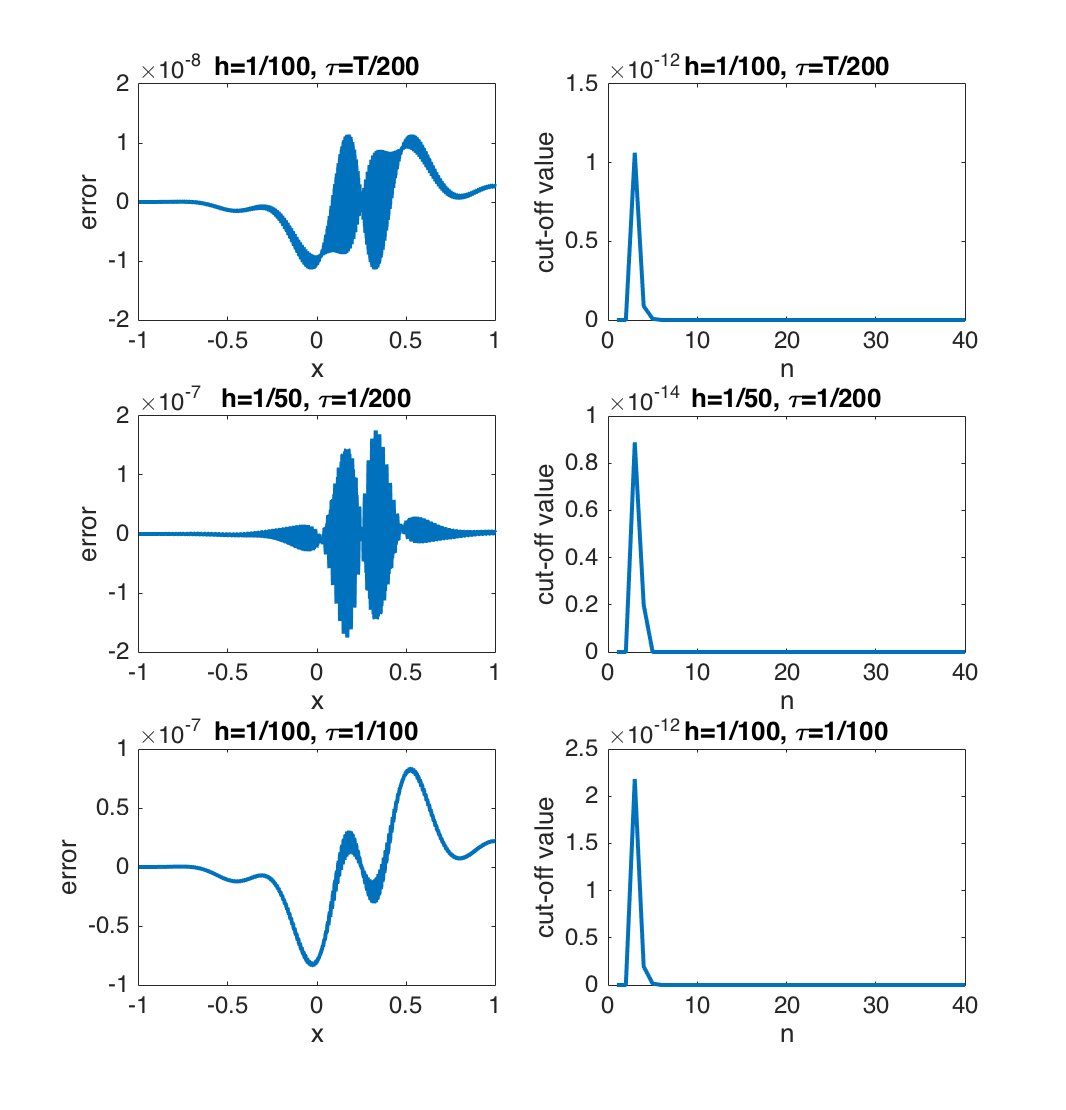
\includegraphics[trim = .1cm .1cm .1cm .1cm, clip=true,width=0.5\textwidth]{ex1_cut.png}
\vspace{-15pt}
\caption{Error at $T=0.01$ and maximal cut-off value at each time level.
\label{fig:err_trun}}
%\vspace{-35pt}
\end{figure}

\begin{figure}[ht]
  \centering
  \subfigure[$m = 1, \epsilon=0.1, T=2, \tau=1/150$]{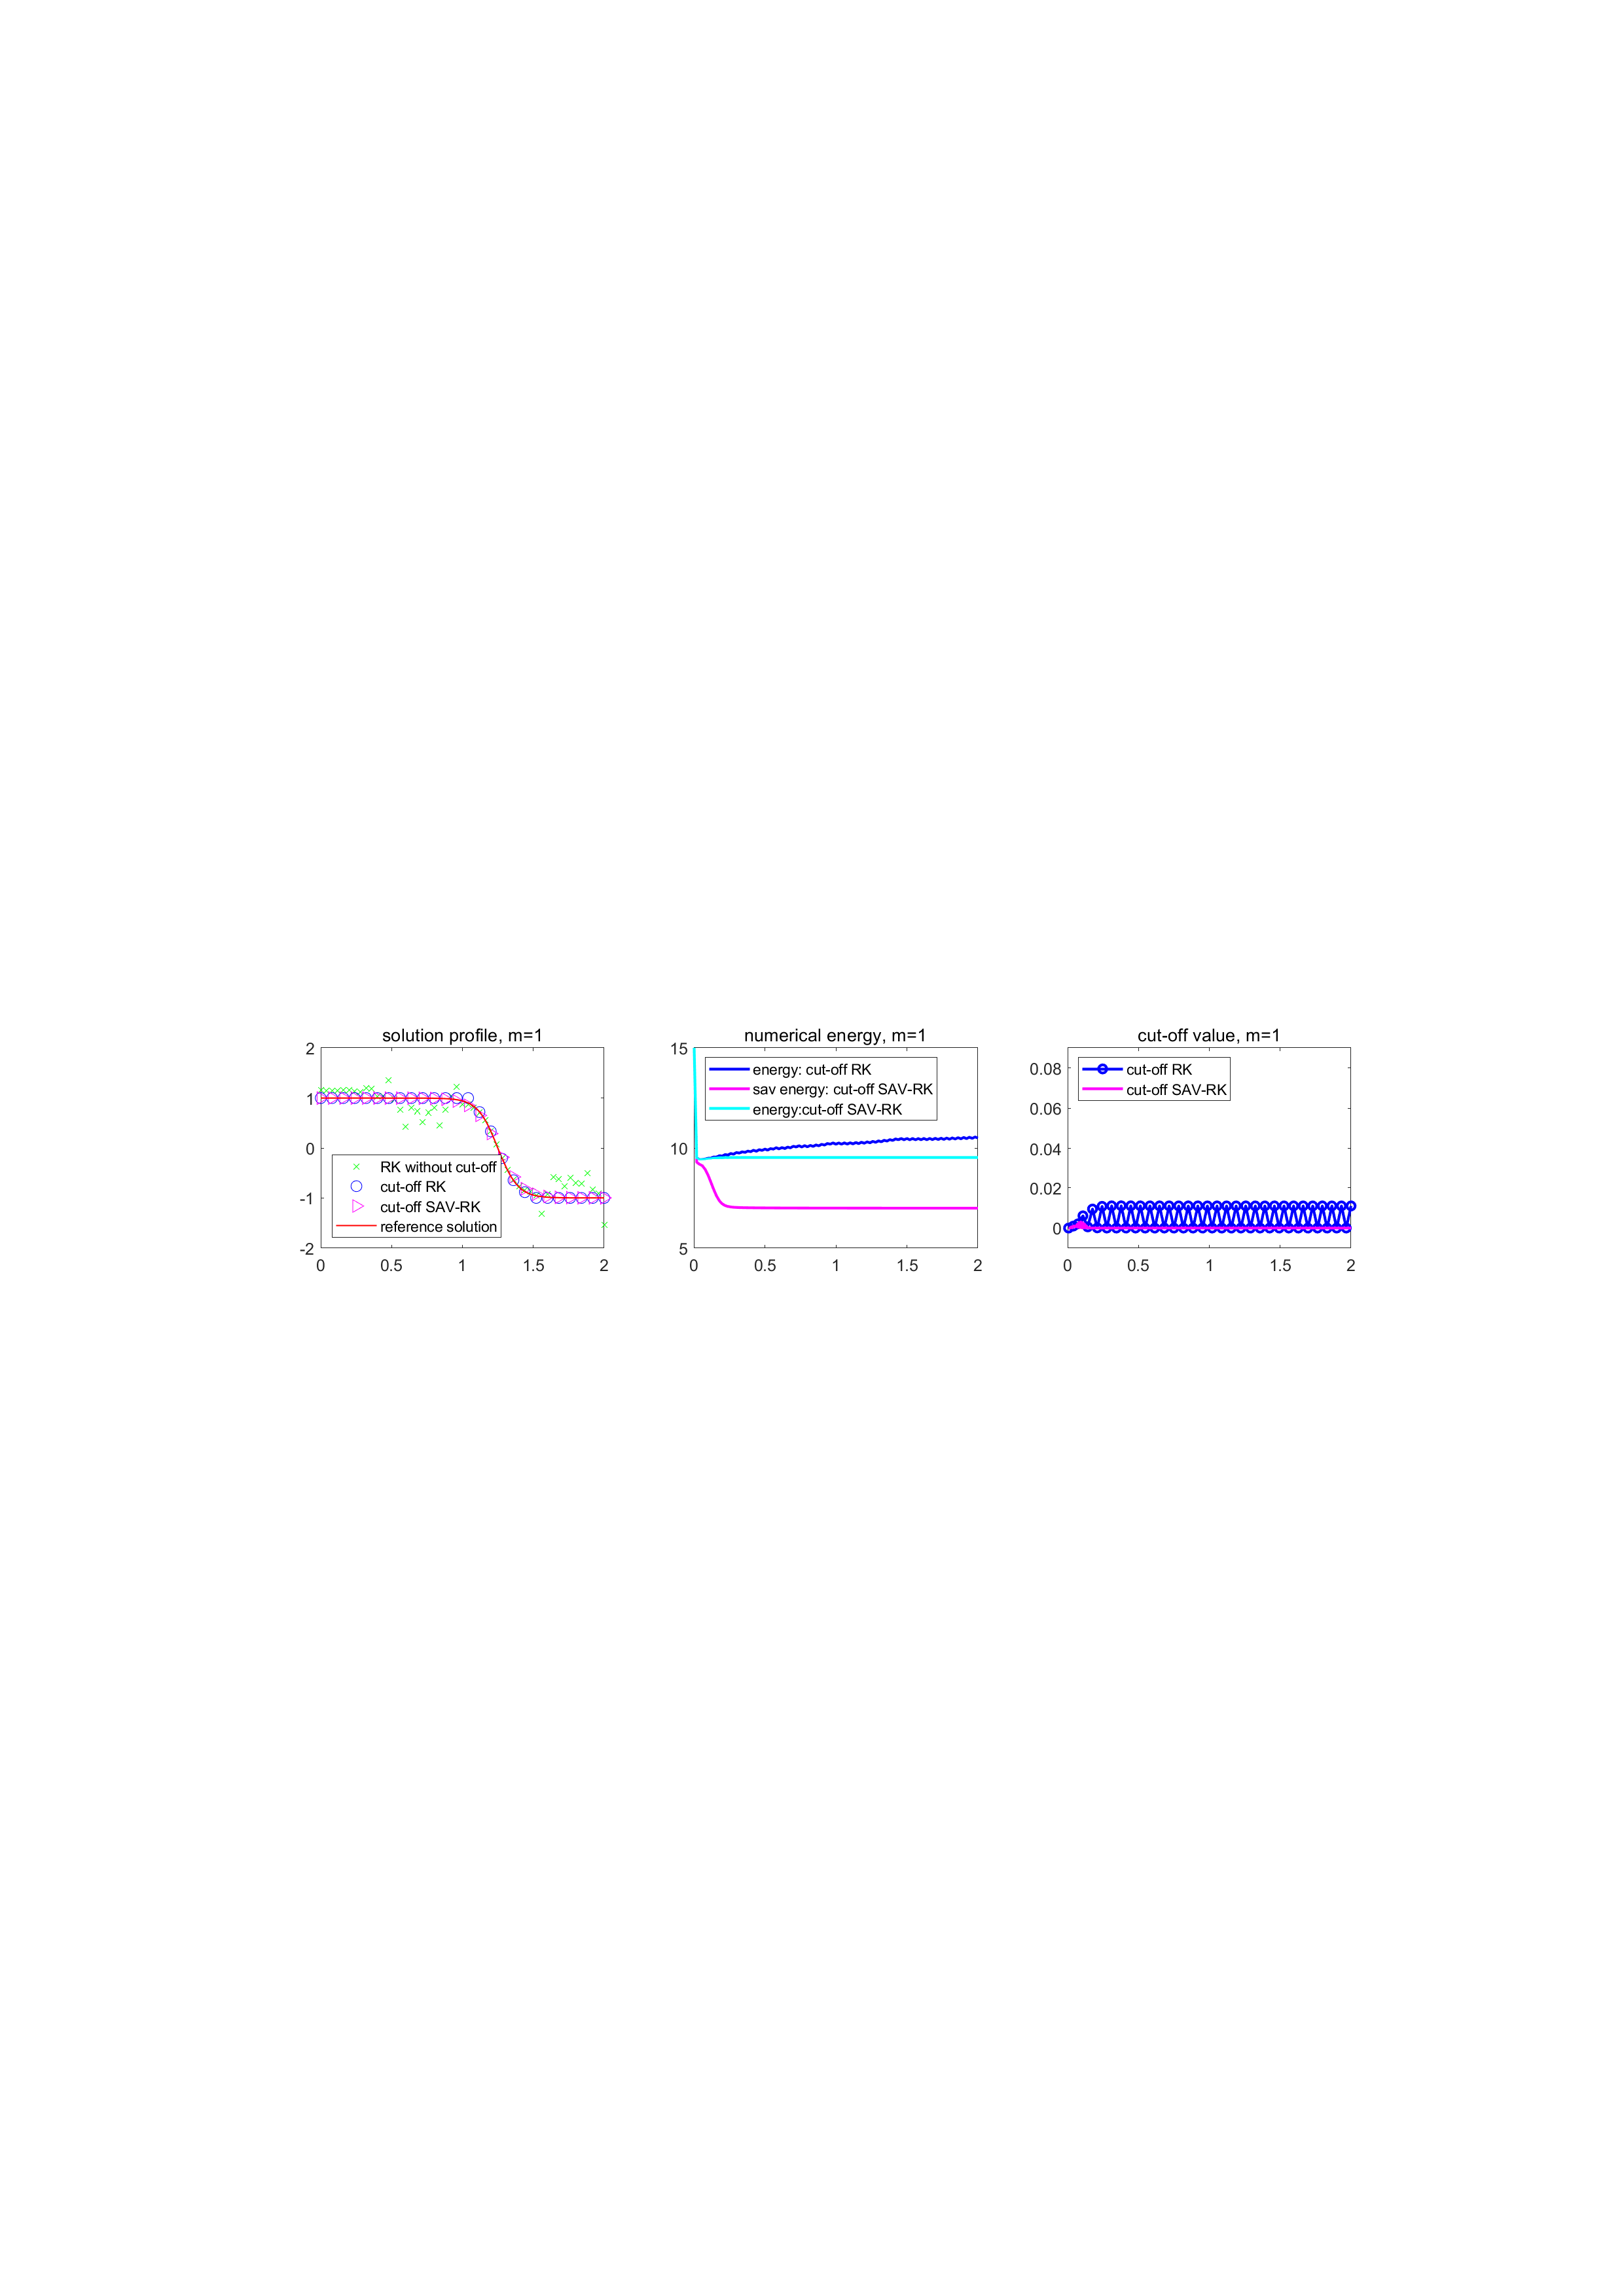
\includegraphics[width=0.8\textwidth]{1d_sol_energy_cut_1_300.pdf}}
  \subfigure[$m = 2, \epsilon=0.1, T=2, \tau=1/250$]{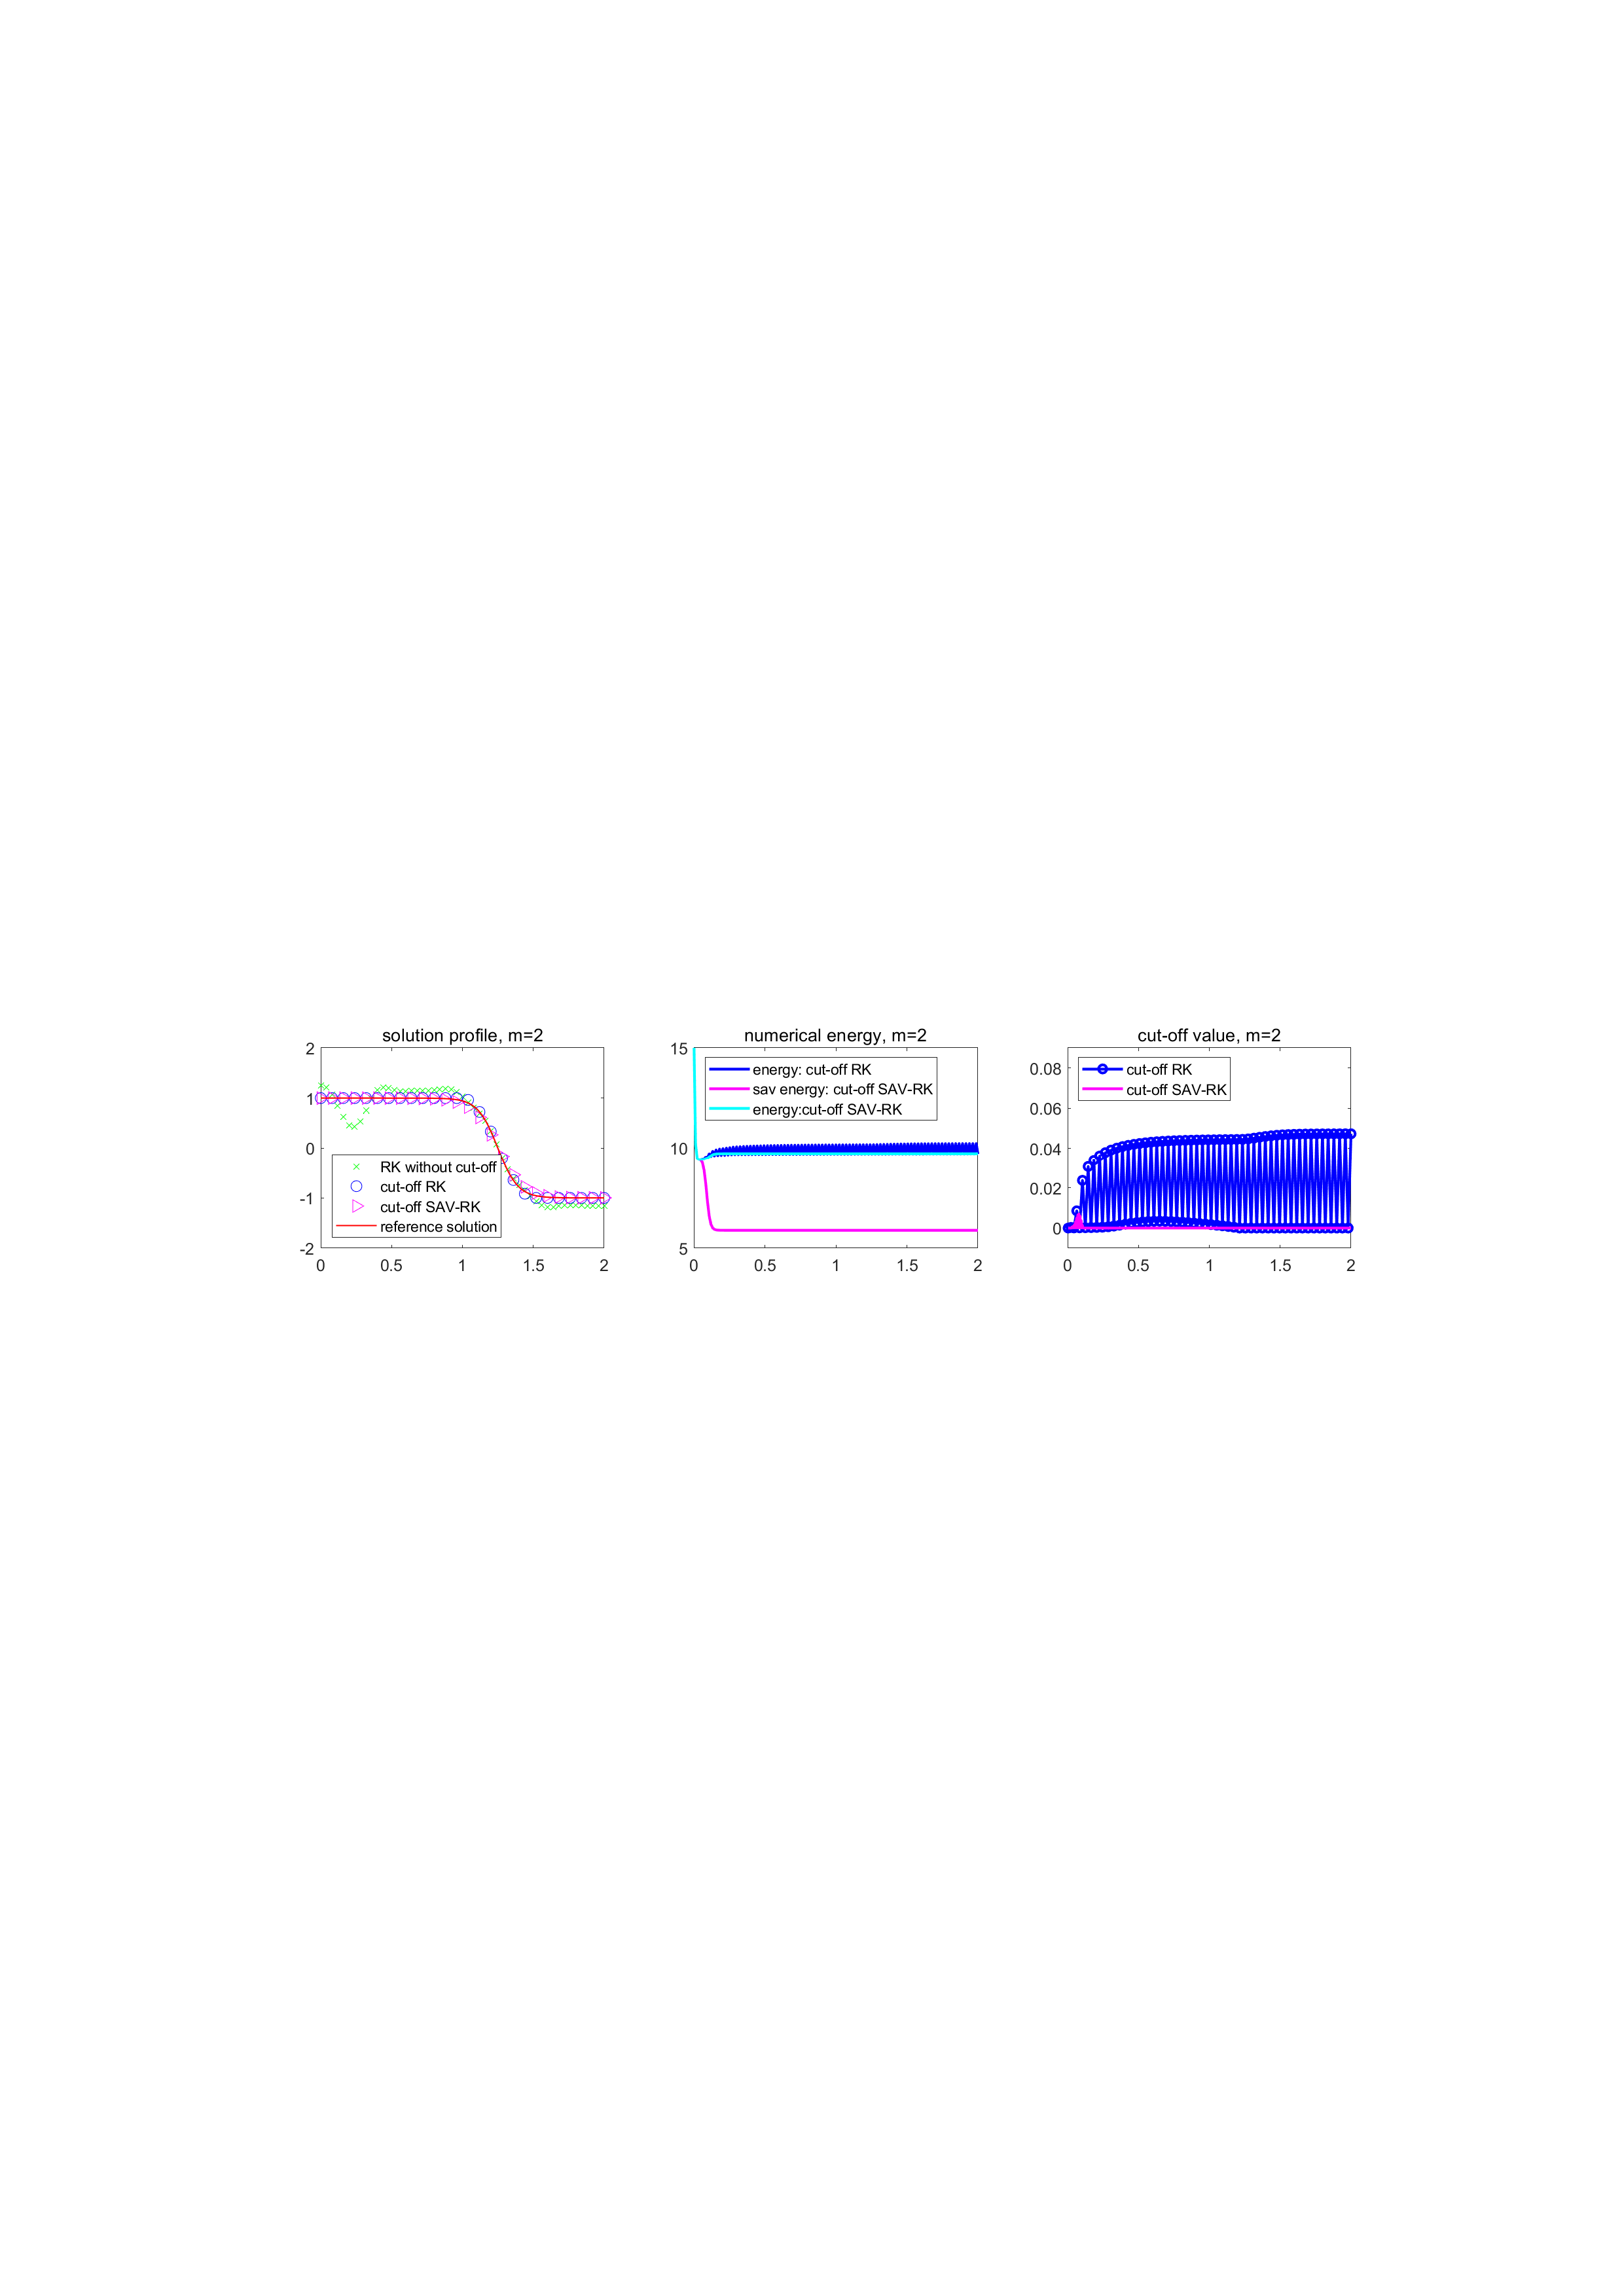
\includegraphics[width=0.8\textwidth]{1d_sol_energy_cut_2_500.pdf}}
%  \subfigure[$m = 3, \epsilon=0.1, T=2, \tau=T/1000$]{\includegraphics[width=\textwidth]{1d_sol_energy_cut_3_1000.pdf}}
  \caption{Left: solution profiles of numerical solutions of RK,  cut-off RK and cut-off SAV-RK scheme.
  Middle: solution energy of cut-off RK and cut-off SAV-RK scheme. Right: cut-off values of cut-off RK and cut-off SAV-RK scheme.}
 \label{fig:energy}
\end{figure}

Finally, we test the numerical results in case of relatively large time steps, and compare the
numerical solutions of extrapolated RK, cut-off RK \eqref{eqn:RK-fully-interpolation}-\eqref{eqn:RK-cut},
 and cut-off SAV-RK schemes \eqref{eqn:AC-sav-fully}-\eqref{eqn:truncation-fully-sav}, with $r=1$,
see Figure \ref{fig:energy}.
Without the cut-off postprocessing, the numerical solutions of RK scheme significantly
exceed the maximum bound,
and present oscillating solution profiles.
With the cut-off operation at each time step, the numerical solutions satisfy the maximum bound,
and present reasonable solution profiles. However,
numerical results show that the cut-off RK scheme
might produce a solution with a obviously increasing and oscillating
energy curve. This issue could be significantly improved by applying the cut-off SAV-RK method, whose solution
satisfy the maximum bound and the numerical energy is more stable.
Moreover, the numerical results show that the cut-off SAV-RK scheme will produce a more regular numerical solution
and smaller cut-off values, compared with the cut-off RK scheme.

\section{Conclusion and Comments}

In this chapter, we discuss the cut-off postprocessing on a series of single step methods, for Allen--Cahn equation with the nonlinear term linearized. We prove that our scheme can be arbitrarily high order for time discretized problem, and be arbitrarily high order for both space and time for fully discretized problem. A lot of famous schemes are included in our analysis. Combining this strategy with SAV technique, we also develop a class of schemes, which preserve both maximum bound and energy stable. Related numerical are also given to corroborate our analysis. 



\chapter{High-order Implicit-Explicit
Runge-Kutta Methods for Parabolic Equations}

In this chapter, we will develop and study Implicit-Explicit Runge--Kutta method (IMEX-RK) for linear and semilinear parabolic equations. To begin with, we will focus on linear non-selfadjoint equations. It is more than a easier case but itself is also a interesting question and related to some physics problems. 

In Section \ref{sec:imex-list}, we will give a brief introduction to the linear problem and its related background. In Section \ref{sec:IMEX} build the IMEX-RK method for linear problem and give its long time error convergence in Section \ref{sec:convergence-imex}. In Section \ref{sec:imex-nonlinear}, we extend the analysis to semilinear problem and show it can keep both maximum bound preserving and original energy decay for up to third order. The schemes of this chapter is listed in Section \ref{sec:imex-list} which meet all our requirements for the convergence. 


\section{Introduction}\label{Sec:intro}\label{Sec:3.1}
In this work, we investigate a numerical approach to solve the following problem. 
Let $V \subset H = H' \subset V'$ be a Gelfand triple of Hilbert spaces, 
where the superscript ' denotes the dual. 
Namely, the embedding $V\embed H$ is continuous and dense, and 
$$(u, v)_{V, V'} = (u,v)_H \quad \forall u \in H \embed V', v \in V \embed H,$$
where $(\cdot, \cdot)_{V, V'}$ is the duality pairing between $V'$ and $V$, 
and $(\cdot,\cdot)_H$ is the inner product on $H$. 

We consider an abstract parabolic initial value problem: 
find
$$u \in L^2((0,T);V) \subset H^1((0,T);V')\embed C([0,T];H)$$\
such that 
\begin{equation}\label{eq:abstract}
    \begin{cases}
    \partial_t u = \calA u + f(t) & 0 < t < T,\\
    u(0) = u_0  \in H
  \end{cases}
\end{equation}
where $\calA: V \to V'$ is a bounded linear operator (possibly non-selfadjoint) 
with the following property that:
\begin{equation}\label{eq:beta}\beta^{-1}\|u\|_V^2 \leq -(\calD u, u) \leq \beta \|u\|_V^2 \quad \forall u \in V, 
\end{equation}
$$ \lvert(\calL u, v)\rvert \leq C \|u\|_V \|v\|_H, 
\forall u\in V, v \in H,$$
where $\calD = (\calA+\calA^*)/2, \calL = (\calA-\calA^*)/2$ are the symmetric and skew-symmetric 
part of the operator $\calA$. Furthermore, $D$ is negative definite. 

\subsection*{The Stokes-Darcy system}
As a multiphysics system, the Stokes-Darcy system is considered in this work which describes a moving fluid governed by the Stokes equations in a free-flow region $\Omega_S\subset\R^d$ and a flow in a neighboring  porous media region $\Omega_D\subset\R^d$. Darcy flow and Stokes flow interact through an interface denoted by $\Gamma$ as shown in Figure \ref{NS_Darcy_domain}. Applications of such a coupled system are ubiquitous in nature, including groundwater system \cite{HoppePortaVassilevski:2007,HouQiuHeGuoWeiBai:2016,LaytonTranTrenchea:2013}, petroleum extraction \cite{ChenSunWang:2014}, and so on.

% the coupling of flow in a porous media region $\Omega_D\subset\R^d$ and a free-flow region $\Omega_S\subset\R^d$ separated by an interface $\Gamma$ (as shown in Figure \ref{NS_Darcy_domain}), which has many applications in groundwater system \cite{JHou_XMHe_CGuo_MWei_BBai_1,RHoppe_PPorta_YVassilevski_1,WLayton_HTran_CTrenchea_1}, industrial filtrations \cite{NHanspal_AWaghode_VNassehi_RWakeman_1,VNassehi_1},  petroleum extraction \cite{TArbogast_MGomez_1,JChen_SSun_XWang_1}, and so on.
\begin{figure}[t]
\begin{center}
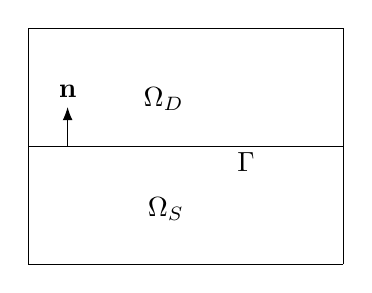
\begin{tikzpicture}
%\draw[-, thick] (0,0) -- (4,0) ;
\draw[-,] (0,0) -- (4,0) ;
\draw[-,] (4,0) -- (4,3) ;
\draw[-, ] (4,3) -- (0,3) ;
\draw[-,] (0,3) -- (0,0) ;
\draw[-] (0,1.5) -- (4,1.5) ;
\draw (2.1,0.7) node[left]{$\Omega_S$} ;
\draw (2.1,2.1) node[left]{$\Omega_D$} ;
\draw (3,1.3) node[left]{$\Gamma$} ;
%\draw[-Latex,] (0.5,1.5) -- (0.5,1.0) node[below]{$\,\,\,\,{\bm n}_D$} ;
\draw[-Latex,] (0.5,1.5) -- (0.5,2.0) node[above]{${\mathbf{n}}$} ;
\end{tikzpicture}
\end{center}
\caption{Computational domain of the Stokes--Darcy system}
%s $\Omega_D$ and $\Omega_S$, and the interface $\Gamma$}
\label{NS_Darcy_domain}
\end{figure}
This model consists of a parabolic equation
\begin{equation}\label{DS-1}
\begin{cases}
\partial_t \phi -\nabla\cdot(\kappa\nabla\phi)  = f_D
&\mbox{in}~~\Omega_D\times(0,T], \\
\phi = 0 &\mbox{on}~~\partial\Omega_D
\backslash\overline\Gamma\times(0,T] ,\\
-\kappa\nabla\phi\cdot \bfn = \u\cdot \bfn   & \mbox{on}~~\Gamma\times(0,T] ,\\
\phi(0)= \phi_0 & \mbox{in}~~\Omega_D,
\end{cases}
\end{equation}
which describes the Darcy flow in the porous media region $\Omega_D$ through the unknown hydraulic head $\phi$,
%(by Darcy's law, the fluid discharge rate is given by $-\kappa\nabla\phi$),
and an evolving Stokes equation
\begin{equation}\label{DS-2}
\begin{cases}
\partial_t \u - \nabla\cdot \T(\u, p )
= \mathbf{f}_S &\mbox{in}~~\Omega_S\times(0,T] , \\
\nabla\cdot\u=0 &\mbox{in}~~\Omega_S\times(0,T] , \\
\u  = 0 &\mbox{on}~~\partial\Omega_S
\backslash\overline\Gamma\times(0,T] ,\\
-\T(\u,p)\bfn = g \phi \bfn +\mu(\bfu-(\bfu\cdot\bfn)\bfn)
& \mbox{on}~~\Gamma\times(0,T] , \\
\u(0)=\u_0 & \mbox{in}~~\Omega_S,
\end{cases}
\end{equation}
which describes free flow in the region $\Omega_S$ through the fluid velocity $\bfu$, where $\T(\u, p)=2\nu \mathbb{D}(\u)-p \mathbb{I}$ denotes the stress tensor, in which $\mathbb{D}(\u)=\frac12(\nabla\u+(\nabla \u)^\top)$ is the deformation tensor and $\mathbb{I}$ is the $d\times d$ identity matrix. The physical parameters $\kappa$, $g$, $\mu$ and $\nu$ in this model are positive constants, and $f_D$ and $\mathbf{f}_S$ are given source terms.

Homogeneous Dirichlet boundary conditions will be imposed on 
outer boundaries separately, i.e., on 
$\partial\Omega_D\backslash\Gamma$ and 
$\partial\Omega_S\backslash\Gamma$. 
The interface conditions on $\Gamma$ in \eqref{DS-1} 
and \eqref{DS-2} represent conservation of mass and 
balance of force, respectively, where $\bfn$ denotes the 
unit normal vector on $\partial\Omega_S$ as shown in Figure 
\ref{NS_Darcy_domain}.

For the ease of error estimate, we will rewrite the Stokes-Darcy system as an equivalent abstract problem.

Let $H= L^2(\Omega_D)\times L^2(\Omega_S)^d$ and $V=H^1_\Gamma(\Omega_D)\times {\bf H}^1_\Gamma(\Omega_S; {\rm div_0})$, where
\begin{align*}
&H^1_\Gamma(\Omega_D)=\{\varphi\in H^1(\Omega_D):\varphi=0\,\,\mbox{on}\,\,\partial\Omega_D\backslash\Gamma\},\\
&{\bf H}^1_\Gamma(\Omega_S; {\rm div_0})=\{{\v}\in H^1(\Omega_S)^d:
\nabla\cdot{\v}=0\,\,\mbox{in}\,\,\Omega_S\,\,\mbox{and}\,\,{\v}=0\,\,\mbox{on}\,\,\partial\Omega_S\backslash\Gamma\}.
\end{align*}
The weak formulation of \eqref{DS-1}-\eqref{DS-2} reads: find $(\phi,\u)\in L^2((0,T);V)\cap H^1((0,T);V') \hookrightarrow C([0,T];H) $
satisfying the following equations for all test functions $(\varphi,{\v})\in L^2((0,T);V)$:
%for all test functions $(\varphi,{\bm v},q)\in H^1(\Omega_D)\times H^1(\Omega_S)^3\times L^2(\Omega_S)$ :
\begin{align}
&(\partial_t\phi,\varphi)_{D}+(\kappa\nabla \phi,\nabla \varphi)_{D}
-(\bfu\cdot\bfn,\varphi)_{\Gamma}=(f_D,\varphi) \label{DS-weak-1} \\[5pt]
&(\partial_t\bfu,{\bfv})_{S}+(2\nu \D(\bfu),\D({\bfv}))_{S}
% - (p,\nabla\cdot{\bm v}) \nonumber \\
+(g\phi,{\bfv}\cdot\bfn)_{\Gamma}
+\mu(\bfu-(\bfu\cdot\bfn) \bfn,{\bfv}-({\bfv}\cdot\bfn) \bfn)_{\Gamma} \label{DS-weak-2} \\
&=(\mathbf{f}_S,{\bfv}) \nonumber ,
%&&\forall\, {\bm v} \in H^1(\Omega_S)^3, \\[5pt]
%&(\nabla\cdot\u,q)_S =0 &&\forall\,q \in L^2(\Omega_S) .
\end{align}
where $(\cdot,\cdot)_D$ is the pairing between $H^1_\Gamma(\Omega_D)'$ and $H^1_\Gamma(\Omega_D)$, $(\cdot,\cdot)_S$ is the pairing between ${\bf H}^1_\Gamma(\Omega_S; {\rm div_0})'$ and ${\bf H}^1_\Gamma(\Omega_S; {\rm div_0})$, and
$(\cdot,\cdot)_\Gamma$ is the inner product on $L^2(\Gamma)$.

Let the operators $A_1:H^1_\Gamma(\Omega_D)\rightarrow H^1_\Gamma(\Omega_D)'$, $A_2:{\bf H}^1_\Gamma(\Omega_S; {\rm div_0})\rightarrow {\bf H}^1_\Gamma(\Omega_S; {\rm div_0})'$, $B:{\bf H}^1_\Gamma(\Omega_S; {\rm div_0})\rightarrow H^1_\Gamma(\Omega_D)'$ and $B^*:H^1_\Gamma(\Omega_D)\rightarrow {\bf H}^1_\Gamma(\Omega_1; {\rm div_0})'$
%\begin{align*}
%&M:H^1(\Omega_D)\rightarrow H^1(\Omega_D)',\\
%&D:{\bf H}^1(\Omega_S; {\rm div_0})\rightarrow {\bf H}^1(\Omega_S; {\rm div_0})',\\
%&B:{\bf H}^1(\Omega_S; {\rm div_0})\rightarrow H^1(\Omega_D)',
%%&B_h:{\bf X}_h^{r+1}(\Omega_S)\rightarrow {\bf X}_h^{r+1}(\Omega_S),\\
%\end{align*}
be defined via duality by
\begin{align*}
&(A_1\phi,\varphi)_D=(\kappa\overline{\nabla\phi},\nabla \varphi)_{D}
\hspace{181pt} \forall\, \phi, \varphi\in H^1_\Gamma(\Omega_D), \\
&(A_2 \u ,{\v} )_S=(2\nu \overline{\D(\u )},\D({\v} ))_{S}\!+\!\mu(\overline{\u\! -\!(\u \cdot\n) \n},{\v}\!-\!({\v} \cdot\n) \n)_{\Gamma}
\hspace{10pt} \forall\,\u ,{\v} \in  {\bf H}^1_\Gamma(\Omega_S; {\rm div_0}) ,\\
&(B \u ,\varphi)_D=(\overline{\u \cdot\n},\varphi )_{\Gamma}
\hspace{33pt}\forall\,\u\in {\bf H}^1_\Gamma(\Omega_S; {\rm div_0}) \hookrightarrow L^2(\Gamma),\,\,\forall\, \varphi \in H^1_\Gamma(\Omega_D) \hookrightarrow L^2(\Gamma),\\
&(B^*\phi, {\v})_D=(\phi,\overline{{\v} \cdot\n} )_{\Gamma}
\hspace{33pt}\forall\,\phi \in H^1_\Gamma(\Omega_D) \hookrightarrow L^2(\Gamma),\,\,\forall\,{\v}\in {\bf H}^1_\Gamma(\Omega_S; {\rm div_0}) \hookrightarrow L^2(\Gamma) .
\end{align*}
Then the weak formulation \eqref{DS-weak-1}-\eqref{DS-weak-2} can be written as
\begin{align}
&\partial_t\phi  +A_1 \phi  - B\u = f_{D} , \label{DS-op1} \\
&\partial_t\u  +A_2 \u + g B^*\phi  = \f_{S} . \label{DS-op2}
\end{align}
By defining notations
\begin{align}
u=\left(\begin{array}{cc}
\phi \\
g^{-\frac12}\u \end{array}\right) ,
\quad
f=\left(\begin{array}{cc}
f_{D} \\
g^{-\frac12}\f_{S} \end{array}\right)
\quad\mbox{and}\quad
\calA
=-\left(\begin{array}{cc}
A_1 &  -g^\frac12B \\
g^{\frac12}B^* &   A_2\end{array}\right) ,
\end{align}
equations \eqref{DS-op1}-\eqref{DS-op2} are equivalently reformulated to the abstract parabolic initial value problem \eqref{eq:abstract}.

Due to the various applications of Stokes-Darcy system, many different numerical methods are developed and analyzed, including domain decomposition methods \cite{DiscacciatiQuarteroni:2004,BoubendirTlupova:2013,CaoGunzburger:2011,ChenGunzburger:2011,DiscacciatiMiglio:2002,DiscacciatiQuarteroni:2007,FengHeWangZhang:2012,GunzburgerHeLi:2018,VassilevWangYotov:2014,QiuHeLiLin:2020}, Lagrange multiplier methods \cite{LaytonFriedhelmYotov:2003,BabuskaGatica:2010,GaticaMeddahiOyarzua:2008,HuangChenCai:2012}, discontinuous Galerkin methods \cite{KanschatRiviere:2010,LipnikovVassilevYotov:2014,Riviere:2005,RiviereYotov:2005}, multigrid methods \cite{ArbogastGomez:2009,MuXu:2008}, partitioned time-stepping methods \cite{KubackiMoraiti:2015,MuZhu:2010,ShanZheng:2013,ZhangRuiCao:2019}, coupled finite element methods \cite{CaoGunzburgerHu,CamanoGatica:2015,KarperMardalWinther:2009,MarquezMeddahiSayas:2015} and many others \cite{ChenGunzburger:2016,ChenGunzburger:2013,GiraultVassilevYotov:2014,HeJiangQiu:2020}. In particular, 
Kubacki et al \cite{kubacki2017non} presented an overview of non-iterative partitioned methods for such a system. With a time-step restriction for stability, numerical schemes of both first-order and high-order partitioned methods were presented. Gunzburger et al in \cite{GunzburgerHeLi:2018} analyzed a parallel, non iterative, multiphysics domain decomposition method for decoupling the Stokes-Darcy model with multistep backward difference formula (BDF) for the time discretization. Optimal order $O(\tau^k)$ for the $k$-step BDF scheme were established in a general framework for any $k\le5$.
Chen et al in \cite{ChenGunzburger:2013} proposed two second-order-in-time implicit-explicit methods including $2$-step BDF and second-order Adams-Moulton-Bashforth method (AME$2$) in which coupling term in the interface conditions was treated explicitly and established for both schemes the unconditional and uniform-in-time stability. Error bound was derived with $O(\tau^2)$.  An improvement of this work was presented in \cite{ChenGunzburger:2016}, in  which a third-order in time AME algorithm was studied and uniform-in-time error estimate was derived.
%Note that all methods are implicit-explicit (IMEX) schemes. 
Recently, authors in \cite{LiWangZhou:2020} presented an implicit-explicit (IMEX) scheme with $k$-step BDF in time and finite element discretization in space. In that paper, the spatial differential operator $\calA$ was split into a symmetric part and an anti-symmetric part on which implicit and explicit schemes were applied respectively. A symmetrized and decoupled temporal $k$-step BDF scheme was presented and optimal long-time error bound $O(\tau^k+h^2)$ was derived.

We notice that aforementioned high-order-in-time works are conducted with multi-step methods and to our knowledge there is no temporal high-order single-step methods adopted for the coupled Stokes-Darcy system in the literature. This motivates us to apply IMEX Runge-Kutta method on the Stokes-Darcy equations aiming to achieve high-order convergence in time.


% \subsection{Our contributions and the organization of the paper}

% In this work, the spatial differential operator is split into symmetric part and skew-symmetric part, on which implicit and explicit Runge-Kutta schemes are applied, respectively. Based on assumptions ({\bf P1})-({\bf P4}) on the scheme, we establish the long-time error bound for the proposed scheme. 

% The rest of this paper is organized as follows.  In Section \ref{sec:IMEX}, we present implicit-explicit Runge-Kutta schemes with various stages and orders and an algorithm for searching coefficients of IMEX Runge-Kutta schemes. Theoretical results for error estimate are shown in Section \ref{sec:convergence-imex}. Finally we present numerical examples in Section \ref{sec:examples} to verify the proposed theorems.





\section{Implicit-Explicit Runge-Kutta Methods}\label{sec:IMEX}

% \subsection{Time-Stepping Schemes}

% To build a time discretization of the equation \eqref{eq:abstract},
% we split the interval $(0, T)$ as
% $$0 = t^0 < t^1 < \cdots < t^n = T,$$
% with the mesh size $\tau := \max_{1\leq i \leq n}\tau_i$ for $\tau_i = t^i - t^{i-1}$.
% Let $u^n$, $u^{n,i}$ are the approximations to $u(t^n)$ and $u(t^{n,i})$ respectively.

% Following Duhamel's principle, the solution of equation \eqref{eq:abstract}
% can be shown as

% $$u(t^n) = e^{\tau_n D}u(t^{n-1}) + \int_0^{\tau_n}e^{(\tau_n-s)D}(Lu(t^{n-1}+s)+f(t^{n-1}+s))\rmd s$$

% Then a framework of a single step scheme of approximating $u(t^n)$ reads:

% \begin{align}\label{eq:SingleStep}
%     u^n = \sigma(-\tau_n D)u^{n-1} + \tau_n \sum_{i=1}^mp_i(-\tau_n D)(L u^{n,i} + f^{n,i})
% \end{align}
% where $t^{n,i} = t^{n-1}  + c_i\tau_n$
% with $c_i$ are distinct real numbers in $[0,1]$ for $i = 1, \dots, m$,
% $u^{n,i}$ is generated from $u^{n-1}$, $f^{n,i} = f(t^{n,i})$. 
% Here $\sigma(\lambda)$ and $\{p_i(\lambda)\}_{i=1}^m$ are rational functions.
% For simplicity reasons, we assume that $\tau^n$ is of uniform mesh size, i.e. $\tau^i = \tau$ for $i = 1, \dots, n$.

% A series of famous schemes are included in this analysis, including the Implicit-Explicit Runge--Kutta scheme
% we are going to talk about.

In this section, we shall propose the time stepping scheme for solving the
Stokes--Darcy system \eqref{DS-1}-\eqref{DS-2} by using the IMEX Runge--Kutta method.
To this end, we split the interval $[0,T]$ into a sequence of subintervals $[t^i, t^{i+1}]$, for $i=0,1,2,\ldots,N-1$.
with time levels $0 = t^0 < t^1 < \cdots < t^n = T$. 
The mesh size is denoted by $\tau := \max_{1\leq i \leq n}\tau_i$ with $\tau_i = t^i - t^{i-1}$.
To simplify the presentation, we will proceed under the assumption that the step size is uniform, i.e., $\tau_i = \tau$ for $i = 1, \dots, n$.
Nevertheless, it is important to note that the analysis applies to nonuniform meshes as well, since the proposed schemes are single-step.



% \subsection{Implicit-Explicit Runge-Kutta schemes}

% For the symmetric part $D$ in equation \eqref{eq:abstract},
% we consider an $m$-stage diagonally implicit Runge--Kutta (DIRK) scheme
% with coefficient $A = \{a_{ij}\}_{m\times m}$, $b = \{b_{i}\}_{i=1}^m$.
% For the skew-symmetric part, we make use of an $m$-stage explicit scheme
% with the same abscissae $\hat{c}=c = \{c_i\}_{i=1}^m$
% and coefficient $\hatA = \{\hata_{ij}\}_{m\times m}$, $\hatb = \{\hatb_{i}\}_{i=1}^m$.
% Thus, the IMEX-RK can be determined by the following Butcher tabular
% % \begin{table}[h]
% %     \centering
% %     \begin{tabular}[h]{c|cccc|cccc}
% %         $c_1$ & $a_{11}$ & $0$ & $\dots$ & $0$ & $\hata_{11}$ & $0$ & $\dots$ & $0$ \\
% %         $c_2$ & $a_{21}$ & $a_{22}$  & $\dots$ & $0$ & $\hata_{21}$ & $\hata_{22}$ & $\dots$ & $0$ \\
% %         $\vdots$ & $\vdots$ & $\vdots$  & $\ddots$ & $\vdots$ & $\vdots$ & $\vdots$ & $\ddots$ & $\vdots$ \\
% %         $c_m$ & $a_{m1}$ & $a_{m2}$  & $\dots$ & $a_{mm}$ & $\hata_{m1}$ & $\hata_{m2}$ & $\dots$ & $\hata_{mm}$ \\
% %         \hline
% %            & $b_1$ & $b_2$ & $\dots$ & $b_m$ & $\hatb_1$ & $\hatb_2$ & $\dots$ & $\hatb_m$
% %     \end{tabular}
% %     \caption{Butcher tableau for Runge--Kutta scheme.}
% %     \label{tab:Butcher}
% % \end{table}



% Then the IMEXRK scheme can be written as

% \begin{equation} \label{eq:imex}
%     \begin{cases}
%         u^{n,0} = u^{n-1}\\
%         u^{n,i} = u^{n-1} + \tau \sum\limits_{j=1}^ia_{ij}Du^{n,j} + \tau \sum\limits_{j=1}^i\hata_{ij}(Lu^{n,j-1}+f(t^{n, j-1})) \quad i = 1, \dots, m\\
%         u^n = u^{n-1} + \tau \sum\limits_{j=1}^m b_jDu^{n,j} + \tau \sum\limits_{j=1}^m \hatb_j(Lu^{n,j-1}+f(t^{n, j-1})) \\
%     \end{cases}
% \end{equation}

% Or, in vector form, let $U^n = \{u^{n,i}\}_{i=1}^m$,
% $V^n =  \{v^{n,i}\}_{i=1}^m =  \{Lu^{n,i-1}+f(t^{n,i-1})\}_{i=1}^m$.
% We can get
% \begin{equation} \label{eq:ImexVec}
%     \begin{cases}
%         U^n = \bbone u^{n-1} + \tau A DU^n + \tau \hatA V^n,\\
%         u^n = u^{n-1} + \tau b^\top D U + \tau b^\top V.
%     \end{cases}
% \end{equation}

% % Ususlly, we can make $b_i$ and $\hatb_i$ be the last column of $A$ and $\hatA$,
% % which means
% % \begin{equation}\label{eq:LastRow}
% %     b^\top = z^\top A, \hatb^\top =  z^\top \hatA.
% % \end{equation}
% % where $z = (0, \dots, 0, 1)^\top$.

% To illustrate the stability, we will make some further assumptions
% to the scheme.
% \begin{itemize}
%     \item[{\bf (P1)}] $\sigma(\lambda)$, $p_i(\lambda)$ are polynomials with respect to $\lambda$ for all $i=1, \dots, m$.
%     $0 < \sigma(\lambda) \leq 1$.
%     Besides, the numerator of $\sigma$ is a polynomial of which the degree is one order lower than its denominator,
%     and the numerators of $p_i$ are polynomials of which the degree are lower than their denominators.
%     \item[{\bf (P2)}] $A = \{a_{ij}\}_{m\times m}$ is lower-triangular, and its diagonal entries $a_{ii}$ are positive for $i\geq 1$.
%     % \item[{\bf (P2)}] $A = \{a_{ij}\}_{m\times m}$ is lower-triangular.
%     \item[{\bf (P3)}] $b_i$ and $\hatb_i$ be the last column of $A$ and $\hatA$, which means that
%     \begin{equation}\label{eq:LastRow}
%         b^\top = z^\top A, \hatb^\top =  z^\top \hatA.
%     \end{equation}
%     where $z = (0, \dots, 0, 1)^\top$.
%     \item[{\bf (P4)}] With the definition
%     $$A_\sigma = \begin{pmatrix}0 & 0 \\ 0 & A \end{pmatrix}, \hatA_\sigma = \begin{pmatrix}0 & 0 \\ \hatA & 0 \end{pmatrix}, b_\sigma =\begin{pmatrix}0 \\ b\end{pmatrix},\hatb_\sigma =\begin{pmatrix}\hatb\\0\end{pmatrix},
%     c_\sigma = \begin{pmatrix}0 \\c\end{pmatrix},$$
%     we have the following properties for given positive integer $k$
%     $${b}_*^\top c^{l-1} = \frac{1}{l}, \text{\quad for $1\leq l \leq k$, ${b}_* \in\{b_\sigma, \hatb_\sigma\}$}$$
%     $$z^\top \left(\prod_{i=1}^{l}A_{*i}\right) e = \frac{1}{l!}, \text{\quad for $1\leq l \leq k$, $A_{*i} \in\{A_\sigma, \hatA_\sigma\}$}$$
%     \begin{equation*}
%         z^\top\left(\prod_{i=1}^{r}A_{*i}\right) c^l = \frac{l!}{(l+r)!}, \quad \forall l\geq 0, r\geq 0, l+r\leq k, A_{*i} \in\{A_\sigma, \hatA_\sigma\}
%     \end{equation*}
% \end{itemize}

% \begin{remark}
%     In condition that assumption (P3) holds, the third relation of 
%     assumption (P4) is a sufficient condition of the other relations. 
% \end{remark}
% Then equation \eqref{eq:ImexVec} gives us
% $$(I - \tau AD)U^n = \bbone u^{n-1} + \tau \hatA V^n,$$
% Take the inverse and employ the last relation of equation \ref{eq:ImexVec},

% $$U^n = (I - \tau AD)^{-1}\bbone u^{n-1} + \tau (I - \tau AD)^{-1}\hatA V^n,$$
% $$u^n = z^\top U^n = z^\top(I - \tau AD)^{-1}\bbone u^{n-1} + \tau z^\top(I - \tau AD)^{-1}\hatA V^n$$


% Let $\sigma(s) = z^\top(I + sA)^{-1}\bbone$,
% and $p_i(s)$ be the $i$-th entry of $z^\top(I + sA)^{-1}\hatA$
% for $s > 0$.
% Then the scheme can also be written as
% \begin{equation}\label{eq:sigma}
%     u^n = \sigma(-\tau D) u^{n-1} + \tau \sum_{i=1}^m p_i(-\tau D)(L u^{n,i-1} + f(t^{n, i-1})).
% \end{equation}

% Later on we will show some properties of $\sigma$ and $p_i$.


% \begin{lemma}\label{thm:Polynomial}
%     If a Runge--Kutta scheme \ref{eq:imex} can be rewritten into \ref{eq:sigma},
%     and the assumption (P2) and (P3) are valid,
%     then all these $\sigma(s)$ and $p_i(s)$ are rational functions with respect to $s$.
%     Their shared denominator is of degree $m$,
%     and their numerators are of degree at most $m-1$.
% \end{lemma}

% Proof:
% To show this, the only point we should focus on is the cofactor matrix
% of $I+sA$. It is well-known that
% $$(I+sA)^{-1} = \det(I+sA)^{-1} (I+sA)^*,$$
% where the star denotes the cofactor matrix.

% Since $\sigma(s) = z^\top(I + sA)^{-1}\bbone$,
% $p_i(s)$ are the $i$-th entry of $z^\top(I + sA)^{-1}\hatA$,
% we can read directly that $\sigma$ and $p_i$
% share the same denominator $\det(I+sA)$, and
% its order is $m$.

% By the definition of the cofactor matrix,
% we can know that all the entries of the cofactor matrix are polynomials of order at most $m-1$,
% So $p_i$and $\sigma$ have their numerators of degree at most $m-1$,
% which completes the proof.

% \begin{corollary}\label{prop:PiSigmaBound}
%     If all the requirements of Lemma \ref{thm:Polynomial} are valid,
%     and Assumption (P1) holds,
%     then there exists positive constants $c_0$, $c_1$, $c_2$, s.t.
%     $$ \sigma(\lambda) < 1/(1+c_0\lambda), \forall \lambda > 0, $$
%     $$ \lambda \sigma(\lambda) < c_1, \forall \lambda > 0, $$
%     $$ p_i(\lambda)\sigma(\lambda)^{-1} < c_2, \forall \lambda > 0. $$
% \end{corollary}

% We list some schemes on the Appendix which satisfy the above assumptions, 
% together with how we can find the schemes. 


For the symmetric part, we consider a $m$-stage diagonally implicit Runge--Kutta (DIRK) scheme
with coefficient $A = \{a_{ij}\}_{m\times m}$, $b = \{b_{i}\}_{i=1}^m$ and $c = \{c_{i}\}_{i=1}^m$.
For the skew-symmetric part, we make use of a $m$-stage explicit scheme
with coefficients $\hatA = \{\hata_{ij}\}_{m\times m}$, $\hatb = \{\hatb_{i}\}_{i=1}^m$ and $\hat{c}=c = \{c_i\}_{i=1}^m$.
It is important to note that the implicit scheme and explicit scheme share the same internal nodes $t^{n,i} = t^{n}+c_i\tau_n$.
The IMEX Runge--Kutta schemes can be determined by the following Butcher tabular
\begin{table} 
    \centering
    \begin{tabular}[h]{c|cccc|cccc}
        $c_1$ & $a_{11}$ & $0$ & $\dots$ & $0$ & $\hata_{11}$ & $0$ & $\dots$ & $0$ \\
        $c_2$ & $a_{21}$ & $a_{22}$  & $\dots$ & $0$ & $\hata_{21}$ & $\hata_{22}$ & $\dots$ & $0$ \\
        $\vdots$ & $\vdots$ & $\vdots$  & $\ddots$ & $\vdots$ & $\vdots$ & $\vdots$ & $\ddots$ & $\vdots$ \\
        $c_m$ & $a_{m1}$ & $a_{m2}$  & $\dots$ & $a_{mm}$ & $\hata_{m1}$ & $\hata_{m2}$ & $\dots$ & $\hata_{mm}$ \\
        \hline
           & $b_1$ & $b_2$ & $\dots$ & $b_m$ & $\hatb_1$ & $\hatb_2$ & $\dots$ & $\hatb_m$
    \end{tabular}
    \caption{Butcher tableau for Runge--Kutta scheme.}
    \label{tab:Butcher}
\end{table}


Throughout, we assume that the scheme is \emph{stiffly accurate}:\vskip5pt

\noindent \textbf{Assumption (P1)} Assume that $b_i$ and $\hat{b}_i$ are the last columns of $A$ and $\hat{A}$, respectively, which means:
    \begin{equation}\label{eq:LastRow}
    b^\top = z^\top A, \quad \hat{b}^\top = z^\top \hat{A}
    \end{equation}
    where $z = (0, \dots, 0, 1)^\top$.

\begin{remark}
The condition (P1) is a common assumption that improves stability when dealing with stiff problems, ensuring that the method can take larger time steps without losing accuracy. See some useful properties in Proposition \ref{thm:Polynomial} and Corollary \ref{prop:PiSigmaBound}.
\end{remark}


Let $u^n$, $u^{n,i}$ be approximations to $u(t^n)$ and $u(t^{n,i})$, respectively, and $f^{n,i} = f(t^{n,i})$. Then the IMEX Runge--Kutta scheme for solving the parabolic problem \eqref{eqn:pde} can be written as
\begin{equation} \label{eq:imex}
    \begin{cases}
        u^{n,0} = u^{n}\\
        u^{n,i} = u^{n} + \tau \sum\limits_{j=1}^ia_{ij} \calD u^{n,j} + \tau \sum\limits_{j=1}^i\hata_{ij}(\calL u^{n,j-1}+f^{n, j-1}) \quad i = 1, \dots, m\\
        u^{n+1} = u^{n} + \tau \sum\limits_{j=1}^m b_j \calD u^{n,j} + \tau \sum\limits_{j=1}^m \hatb_j(\calL u^{n,j-1}+f^{n, j-1}). \\
    \end{cases}
\end{equation}
Alternatively, we let $U^n = (u^{n,i})_{i=1}^m$,
$V^n =  (v^{n,i})_{i=1}^m =  (\calL u^{n,i-1}+f^{n,i-1})_{i=1}^m$.
Then the scheme \eqref{eq:imex} could be written in vector form as
\begin{equation} \label{eq:ImexVec}
    \begin{cases}
        U^n = \bbone u^{n} + \tau A \calD U^n + \tau \hatA V^n,\\
        u^{n+1} = u^{n} + \tau b^\top \calD U^n + \tau b^\top V^n.
    \end{cases}
\end{equation}
Note that the first relation in \eqref{eq:ImexVec} leads to
$$U^n = (I - \tau A\calD)^{-1} (\bbone u^{n} + \tau \hatA V^n).$$
This together with the second relation in \eqref{eq:ImexVec} and Assumption (P1) yields
\begin{equation}\label{eqn:vect}
\begin{aligned}
 u^{n+1} = z^\top U^n = z^\top(I - \tau A\calD)^{-1}\bbone u^{n} + \tau z^\top(I - \tau A\calD)^{-1}\hatA V^n
\end{aligned}
\end{equation}
where $z = (0, \dots, 0, 1)^\top$.
Let $\sigma(s) = z^\top(I + sA)^{-1}\bbone$,
and $p_i(s)$ be the $i$-th entry of $z^\top(I + sA)^{-1}\hatA$
for $s > 0$.
Then the scheme \eqref{eqn:vect} can  be written as the following equivalent form 
\begin{align}\label{eqn:SingleStep}
    u^{n+1} = \sigma(-\tau_n \calD)u^{n} + \tau_n \sum_{i=1}^mp_i(-\tau_n \calD)(\calL  u^{n,i} + f^{n,i}).
\end{align}
Here $\sigma(s)$ and $\{p_i(s)\}_{i=1}^m$ are rational functions.


To guarantee long-time stability, we need the following assumption on the rational function $\sigma$.\vskip5pt

\noindent \textbf{Assumption (P2):} We assume that $0 < \sigma(s) < 1$ for all $s\in(0,\infty)$.

\begin{remark}\label{rem:P2} 
The bound $|\sigma(s)| \le 1$ is typically required for stability. However, we need a stronger assumption, $\sigma(s) > 0$, to ensure that $\sigma(-\tau \mathcal{D})$ is invertible. This is crucial because we use the test function $\sigma(-\tau \mathcal{D})^{-1} u^{n+1}$ in the proof of long-time stability (see Theorem \ref{thm:Stable}). For the backward Euler scheme, $\sigma(-\tau \mathcal{D})^{-1} = (\mathcal{I} - \tau \mathcal{D})$ is well-defined, but the invertibility of $\sigma(-\tau \mathcal{D})$ is not always guaranteed for higher-order Runge--Kutta methods.
\end{remark}

Later on, we will show some properties of $\sigma$ and $p_i$, which will benefit our further analysis. 

\begin{proposition}\label{thm:Polynomial}
Assume that (P1) is valid. Then $\sigma$ and $p_i$ possess a common denominator with a degree of $m$, while the degree of their numerators does not exceed $m-1$.
\end{proposition}

\begin{proof}
Note that $(I+sA)^{-1} = (\det(I+sA))^{-1}(I+sA)^*$, where the star here denotes the cofactor matrix.
Since $\sigma(s) = z^\top(I + sA)^{-1}\bbone$ and 
$p_i(s)$ are the $i$-th entry of $z^\top(I + sA)^{-1}\hatA$,
we observe that $\sigma$ and $p_i$ share the same denominator $\det(I+sA)$, a polynomial of degree $m$.
Also, we conclude that all entries of the cofactor matrix are polynomials with degree not exceeding $m-1$.
It follows that numerators of the polynomials 
$p_i$ and $\sigma$ also have a degree of $m-1$. 
\end{proof}


As a direct result of Proposition \ref{thm:Polynomial}, we have the following estimates for the rational functions $\sigma$ and $p_i$.
\begin{corollary}\label{prop:PiSigmaBound}
Let Assumptions (P1) and (P2) be valid.  Then there exist positive constants $c_0$, $c_1$ and $c_2$  such that for all $s \ge 0$, the following holds:
\begin{equation*} 
\begin{aligned} 
\sigma(s) < \frac{1}{1+c_0s}, \quad  
 s \sigma(s)  < c_1 \quad \text{and} \quad
 \left\lvert \frac{p_i(s)}{\sigma(s)} \right\rvert< c_2 .
 \end{aligned}
\end{equation*}
\end{corollary}
\begin{proof}
In the first estimate, $(1+cs)\sigma(s)$ is a rational function with equal numerator and denominator, finite on $(0, \infty)$. It has finite local maxima on this interval. For $c=0$, all maxima are less than one, so there exists a small $c_0$ near zero such that $(1+cs)\sigma(s) < 1$.

In the second estimate, $s\sigma(s)$ is a rational function where the numerator equals the denominator, making it finite on $(0, \infty)$. Therefore, $\lim_{s \to +\infty} s\sigma(s)$ is finite, and $s\sigma(s)$ remains finite on $(0, \infty)$.

In the third estimate, ${p_i}/{\sigma}$ is a rational function where the numerator equals the denominator, ensuring it is finite on $(0, \infty)$ and remains finite throughout. 

\end{proof}

 To illustrate the order condition of our scheme, we need to make the third assumption: 

\noindent\textbf{Assumption (P3)} 
Here we define
$$A_+ = \begin{pmatrix}0 & 0 \\ 0 & A \end{pmatrix}, \hatA_+ = \begin{pmatrix}0 & 0 \\ \hatA & 0 \end{pmatrix}, 
%b_+ =\begin{pmatrix}0 \\ b\end{pmatrix},\hatb_+=\begin{pmatrix}\hatb\\0\end{pmatrix},
c_+ = \begin{pmatrix}0 \\c\end{pmatrix}.$$
We assume that, for a given positive integer $k$, the following properties hold valid
\begin{equation}\label{eq:ass_p3}
    z^\top( A_*)^{r+1} c_+^l = \frac{l!}{(l+r+1)!}, \quad \forall l\geq 0, r\geq 0, l+r\leq k-1,
\end{equation}
where, each appearance of $A_*$ during the multiplication is either $\As$ or $\Ahs$. 
    
    


We say a scheme is accurate of order $k$, if
\begin{subequations}
\begin{equation}\label{eq:Append_Acc1}
    \sigma(\lambda) = e^{-\lambda} + O(\lambda^{k+1}) \mbox{ as }\lambda \to 0, 
\end{equation}
and, for any $0\leq l \leq k$, 
\begin{equation}\label{eq:Append_Acc2}
    \sum_{i=0}^m c_i^lp_i(\lambda) = \frac{l!}{(-\lambda)^{l+1}}
    \Big(e^{-\lambda} -\sum_{l=0}^j \frac{(-\lambda)^l}{l!}\Big)
    + O(\lambda^{k-l}) \mbox{ as }\lambda \to 0. 
\end{equation}
\end{subequations}
To achieve $k$-th order accuracy, the following theorem provides the necessary and sufficient conditions for the Butcher tableau.
\begin{theorem}
The scheme is accurate of order $k$ for linear symmetric problem if Assumption (P3) is valid. 
\end{theorem}
\begin{proof}
Let $\calA = \calD$ and denote $U^n = \{u^{n,i}\}_{i=0}^m$ and
$F^n =  \{f(t^{n,i})\}_{i=0}^m$.
Then scheme reads
\begin{equation} \label{eq:AppendImexVec}
        U^n = \bbone u^{n} + \tau \As \calD U^n + \tau \Ahs F^n\quad \text{and}\quad 
        u^{n+1} = u^{n} + \tau \bs^\top \calD  U + \tau \bs^\top F.
\end{equation}
The first relation of \eqref{eq:AppendImexVec} gives 
%$$(I-\tau \As \calD )U^n = \bbone u^{n} + \tau \Ahs F^n, $$
$$U^n = (I-\tau \As \calD )^{-1}\bbone u^{n} + \tau (I-\tau \As \calD )^{-1}\Ahs F^n.$$
The equation \eqref{eq:LastRow} guarantees that 
the last element of $U^n$ happens to be $u^{n+1}$ itself, 
so finally we can get
$$u^{n+1} = \sigma(-\tau \calD )u^{n} + \tau \sum_{i=0}^mp_i(-\tau \calD )f(t^{n,i}), $$
where $\sigma(\lambda) = z^\top (1+\lambda \As)^{-1}\bbone$, 
$\{p_i(\lambda)\}^\top = z^\top (1+\lambda \As)^{-1} \Ahs $
for $\lambda \geq 0$. 
We know the rational real function on the operator $\calD $ is 
well-defined since $\calD$ is negative definite such that $-\tau \calD$ is positive definite. 





To derive \eqref{eq:Append_Acc1}, since the rational functions and 
exponential functions are sufficiently smooth and analytic, we can just take the derivative and
test whether they are the same at zero. 
$$\left(\frac{\rmd}{\rmd \lambda}\right)^l\sigma = z^\top \left(\left(\frac{\rmd}{\rmd \lambda}\right)^l (1+\lambda \As)^{-1}\right)\bbone
=(-1)^l l! z^\top (1+\lambda \As)^{-(l+1)}\As^l\bbone. $$
Therefore, \eqref{eq:Append_Acc1} is true if and only of
$$\left(\frac{\rmd}{\rmd \lambda}\right)^l\sigma(0) = (-1)^l l! z^\top \As^l \bbone = (-1)^l, \quad \forall 0\leq l \leq k,$$
which means 
$$  z^\top \As^l \bbone = \frac{1}{l!}, \quad \forall 0\leq l \leq k.$$

To evaluate \eqref{eq:Append_Acc2}, 
we need some simplification.
The equation \eqref{eq:Append_Acc2} is equivalent to 
\begin{equation}\label{eq:Append_Acc2b}
    (-\lambda)^{l+1}\sum_{i=0}^m c_i^lp_i(\lambda) = l!
    \Big(e^{-\lambda} -\sum_{l=0}^j \frac{(-\lambda)^l}{l!}\Big)
    + O(\lambda^{k+1}), \quad as~\lambda \to 0. 
\end{equation}
Similarly, we only need to compare their derivatives at zero. 
Let $$LHS =  (-\lambda)^{l+1}\sum_{i=0}^m c_i^lp_i(\lambda),\quad RHS = l!
\Big(e^{-\lambda} -\sum_{l=0}^j \frac{(-\lambda)^l}{l!}\Big).$$
It is obviously that $LHS$ has a $\lambda^{l+1}$ factor 
so it is zero for no more than $l$-th order derivative. 
So does $RHS$ because it is 
the Taylor's expansion. 
Thus we only need to test their derivatives with order 
more than $l$.

Let $r\geq 0$ and $l+1+r = k$. Taking the $(l+1+r)$-th order 
derivative on $LHS$, with the Leibniz product rule, 
we can derive that
\begin{align*}
{\left(\frac{\rmd}{\rmd \lambda}\right)}^{l+1+r}LHS(0)
&= C_{l+1+r}^r {\left(\frac{\rmd}{\rmd \lambda}\right)}^{l+1} (-\lambda)^{l+1} {\left(\frac{\rmd}{\rmd \lambda}\right)}^r\sum_{i=0}^m c_i^lp_i(\lambda) \\
&= \frac{(l+1+r)!}{(l+1)!r!}(-1)^{l+1}(l+1)!\cdot
z^\top (-1)^r r! (1+ 0 \cdot  \As)^{-(r+1)} \As^r \Ahs c^l\\
&= (-1)^{l+1+r}(l+1+r)!z^\top\As^r\Ahs c^l.
\end{align*}
    
Therefore, \eqref{eq:Append_Acc2} is true if and only if
$$(-1)^{l+1+r}(l+1+r)!z^\top\As^r\Ahs c^l = (-1)^{l+1+r}(l)!, \quad \forall l\geq 0, r\geq 0, l+r\leq k-1, $$
which means 
$$   z^\top\As^r\Ahs c^l = \frac{l!}{(l+r+1)!}, \quad \forall l\geq 0, r\geq 0, l+r\leq k-1.
$$
That is guaranteed by the assumption. 
\end{proof}


\begin{remark}
    If the source term is partially or fully computed implicitly, 
    then an additional requirement
    \begin{equation*}
        z^\top\As^r\As c^l = \frac{l!}{(l+r+1)!}, \quad \forall l\geq 0, r\geq 0, l+r\leq k-1
    \end{equation*}
    should be added.
The proof is a line-by-line copy of the previous one.
\end{remark}



\section{Implicit-Explicit Runge--Kutta Methods for Linear Problems}\label{sec:convergence-imex}

Before we illustrate the stability theorem, we will show a stability lemma for the stages, which may be used in the later theorem.
\begin{lemma}\label{thm:Stages}
    If a series of solutions satisfy
    $$\psi = \phi + c_0 \tau \calD\psi + \tau \sum\limits_{i=1}^{m}a_{i}Dv^i + \tau \sum\limits_{i=1}^{m}\hata_{i}\calL v^{i},$$
    for some constant $c_0>0$, then there exists a constant $C$ such that
    $$\|\psi\|_H \leq C\Big( \|\phi\|_H + \sum_{i=1}^m \|v_i\|_H \Big)
    \quad \text{and}\quad \|\psi\|_V \leq C\Big( \|\phi\|_V + \sum_{i=1}^m \|v_i\|_V \Big),$$
\end{lemma}
\begin{proof}Take the inverse of $(I - c_0 \tau\calD)$, we can get

$$\psi = (I - c_0 \tau\calD)^{-1}\Big(\phi + \tau \sum\limits_{i=1}^{m}a_{i}\calD v^i\Big) + \tau \sum\limits_{i=1}^{m}\hata_{i}(I - c_0 \tau \calD)^{-1}Lv^{i}.$$
Test with $\psi$ and we can get
$$\|\psi\|_H^2 \leq C\|\psi\|_H\Big(\|\phi\|_H + \sum_{i=1}^m \|v_i\|_H\Big) + \tau \sum\limits_{i=1}^{m} \hata_i\Big(\calL v^{i}, (I - c_0 \tau \calD)^{-1} \psi\Big)$$
and
$$\tau \Big(\calL v^{i}, (I - c_0 \tau \calD)^{-1} \psi\Big) \leq C \tau \|v^i\|_H \|(I - c_0 \tau \calD)^{-1} \psi\|_V \leq C \|v^i\|_H \|\psi\|_H.$$
which gives us the first relation.

To get the second relation, instead of test $\psi$, we will now test $-D\psi$ to the above equation. It turns to be
$$\|\psi\|_V^2 \leq C\|\psi\|_V\Big(\|\phi\|_V + \sum_{i=1}^m \|v_i\|_V\Big) - \tau \sum\limits_{i=1}^{m} \hata_i\Big(\calL v^{i}, \calD(I - c_0 \tau \calD)^{-1} \psi\Big)$$
and
$$\tau \Big(\calL v^{i}, \calD(I - c_0 \tau \calD)^{-1} \psi\Big) \leq  C\tau \|v^i\|_V \|\calD(I - c_0 \tau \calD)^{-1} \psi\|_H \leq C \|v^i\|_V \|\psi\|_V.$$
which gives us the second relation.
\end{proof}

\begin{theorem}\label{thm:Stable}
    If $u^i$ and $u^{n,i}$ are the solutions generated by \ref{eq:imex},
    with $f=0$, and the Assumption (P1) (P2) hold,
    then
    $$\|u^n\|_H^2  \leq \|u^{n-1}\|_H^2 , \forall n>1$$
    when $\tau \leq \tau^*$, 
    where the constant $\tau^*$ is only 
    related to the scheme and $\beta$ in equation \eqref{eq:beta}, 
    and not related to $u$ or $u^n$.
\end{theorem}
\begin{proof} 
Test equation \ref{eqn:SingleStep} with $\sigma^{-1}(-\tau \calD)u^n$, we can get

$$\big(u^n, \sigma^{-1}u^n\big) = \big(\sigma u^{n-1}, \sigma^{-1}u^n\big) +\tau \sum_{i=1}^m \big(p_i\calL u^{n,i-1}, \sigma^{-1}u^n\big)$$

Due to the symmetry of $D$, all the rational combinations are symmetric and commutable, so 

$$\big(u^n, \sigma^{-1}u^n\big) = \big( u^{n-1}, u^n\big) +\tau \sum_{i=1}^m  \big(\calL u^{n,i-1},p_i \sigma^{-1}u^n\big)$$

Since $\calL$ is skew-symmetric, $(\alpha \calL w,w) = \alpha(\calL w, w)=-\alpha(w, \calL w) = 0$ for all $\alpha, w$,
so
$$\big(u^n, \sigma^{-1}u^n\big)  = \big( u^{n-1}, u^n\big) +
\tau \sum_{i=1}^m  \bigg(\calL\big(u^{n,i-1}-p_i(0)^{-1}p_i \sigma^{-1}u^n\big),p_i \sigma^{-1}u^n\bigg).$$

For our assumption, there exist an $c_0' = c_0 /\beta$ s.t. $0 < \sigma(s) <1/(1+c_0'\beta s)$, so the LHS
of the above equation can be bounded by

$$\big(u^n, \sigma^{-1}u^n\big) > \big\|u^n\big\|_H^2 + c_0'\tau\big\|u^n\big\|_V^2$$

and
$$\big(u^{n-1}, u^n\big) = \frac12\big\|u^n\big\|_H^2+\frac12\big\|u^{n-1}\big\|_H^2-\frac12\big\|u^n-u^{n-1}\big\|_H^2.$$

For the second term on the RHS, use the property of $L$, we can get

\begin{align*}
\sum_{i=1}^m & \;\bigg(\calL\big(u^{n,i-1}-p_i(0)^{-1}p_i \sigma^{-1}u^n\big),p_i \sigma^{-1}u^n\bigg)\\
&\leq \epsilon \sum_{i=1}^m\big\|p_i \sigma^{-1}u^n\big\|_V^2
+ C_\epsilon \sum_{i=1}^m\big\|u^{n,i-1}-p_i(0)^{-1}p_i \sigma^{-1}u^n\big\|_H^2\\
&\leq \epsilon \sum_{i=1}^m\big\|p_i \sigma^{-1}u^n\big\|_V^2
+ 2C_\epsilon \sum_{i=1}^m\big\|u^{n,i-1}-u^n\big\|_H^2 +2C_\epsilon \sum_{i=1}^m\big\|u^n-p_i(0)^{-1}p_i \sigma^{-1}u^n\big\|_H^2\\
&=I_1+I_2+I_3
\end{align*}

By corollary \ref{prop:PiSigmaBound}, we can get
$$I_1 = \epsilon \sum_{i=1}^m\big\|p_i \sigma^{-1}u^n\big\|_V^2 < \epsilon_1 C \big\|u^n\big\|_V^2.$$

% The estimation of $I_2$ is more tricky.
% Reformulate the first relation of \ref{eq:ImexVec}
% and we can get
% \begin{align}\label{eq:ProofStable2}
%     U^n - u^n\bbone  = (u^{n-1}-u^n)\bbone  + \tau A D(U^n-u^n\bbone) + \tau \hatA (V^n-Lu^n\bbone )
% + \tau(AD+\hatA L)u^n \bbone.
% \end{align}
% Test it with $U^n - u^n\bbone$.
% $$\big(U^n - u^n\bbone\big)^\top \big(u^{n-1}-u^n\big)\bbone \leq \epsilon_{21} \sum_{i=1}^m \big\|u^{n,i}-u^n\big\|_H^2 + C_{21}\big\|u^{n-1}-u^n\big\|_H^2$$
% $$\big(U^n - u^n\bbone\big)^\top\tau A D\big(U^n-u^n\bbone\big) \leq \tau C_A \sum \big\|u^{n,i}-u^n\big\|_V^2$$
% $$\big(U^n - u^n\bbone\big)^\top\tau \hatA \big(V^n-Lu^n\bbone \big)\leq \tau C_\hatA \sum \big\|u^{n,i}-u^n\big\|_V^2 + \tau C_\hatA \sum \big\|u^{n,i}-u^n\big\|_H^2$$
% $$\big(U^n - u^n\bbone\big)^\top\tau AD u^n \bbone \leq \epsilon_{22} \big\|u^n\big\|_V^2 +  \tau^2 C_{22}\sum \big\|u^{n,i}-u^n\big\|_V^2 $$
% $$\big(U^n - u^n\bbone\big)^\top\tau \hatA L u^n \bbone \leq \epsilon_{23} \big\|u^n\big\|_V^2 +  \tau^2 C_{23}\sum \big\|u^{n,i}-u^n\big\|_H^2 $$

% Combine all these terms, for fixed small $\epsilon_{2i}$, and make $\tau < \tau_1^*$
% which is only related to $\epsilon_{2i}$ and $\hatA$,
% then the terms $\|u^{ni}-u^n\|^2$ of the RHS can partially cancel the LHS, then
% $$I_2 \leq C_1\epsilon_2 \big\|u^n\big\|_V^2 + C_1C_2\big\|u^{n-1}-u^n\big\|_H^2
% +\tau CC_1 \sum\big\|u^{n,i}-u^n\big\|_V^2$$

Then we are going to estimate $I_2$. The second relation in \ref{eq:imex} gives us
$$u^{n,i}-u^n = (u^{n-1}-u^n) + \tau \sum\limits_{j=1}^ia_{ij}\calD(u^{n,j}-u^n) + \tau \sum\limits_{j=1}^i\hata_{ij}\calL(u^{n,j-1}-u^n) + \tau c_i(\calD+\calL)u^n.$$

Define $w^{n,i} = u^{n,i}-u^n$, so
$$w^{n,i} = w^{n,0} + \tau \sum\limits_{j=1}^ia_{ij}\calD w^{n,j} + \tau \sum\limits_{j=1}^i\hata_{ij}\calL w^{n,j-1} + \tau c_i(\calD+\calL)u^n.$$

Similar with Lemma \ref{thm:Stages}, taking the inverse of $\big(I-a_{ii}\tau \calD\big)$, we can derive that

\begin{align*}w^{n,i} &= \tau \sum\limits_{j=1}^{i-1}a_{ij}\big(I-a_{ii}\tau \calD\big)^{-1}\calD w^{n,j} 
+ \tau \sum\limits_{j=1}^i\hata_{ij}\big(I-a_{ii}\tau \calD\big)^{-1}\calL w^{n,j-1} \\
&+ \big(I-a_{ii}\tau \calD\big)^{-1}w^{n,0} 
+ \tau c_i\big(I-a_{ii}\tau \calD\big)^{-1}\calD u^n+ \tau c_i\big(I-a_{ii}\tau \calD\big)^{-1}\calL u^n. 
\end{align*}



Test with $w^{n,i}$, we can derive that 
\begin{align*}\|w^{n,i}\|_H^2 &\leq C \sum\limits_{j=1}^{i-1}a_{ij}\|w^{n,j}\|_H^2 
+ \tau \sum\limits_{j=1}^i\hata_{ij}\big(\calL w^{n,j-1},\big(I-a_{ii}\tau \calD \big)^{-1} w^{n,i} \big)\\
&+ \|w^{n,0}\|_H\|w^{n,i}\|_H + C\tau^{1/2} \|u^n\|_V\|w^{n,i}\|_H+ \tau c_i\big(\calL u^n, \big(I-a_{ii}\tau \calD\big)^{-1}w^{n,i}\big),
\end{align*}
and
$$\big(\calL\phi,\big(I-a_{ii}\tau \calD\big)^{-1} \chi \big) 
\leq C\|\phi\|_H\|\big(I-a_{ii}\tau \calD\big)^{-1} \chi\|_V
\leq C\|\phi\|_H\|\chi\|_H,$$
for any $\phi, \chi$. 
Therefore
$$\|w^{n,i}\|_H \leq C \|w^{n,0}\|_H + C \sum\limits_{j=1}^{i-1}a_{ij}\|w^{n,j}\|_H+C \tau^{1/2}\|u^n\|_V.$$

Accumulate from $1$ to $i$, we can derive that
$$\|w^{n,i}\|_H \leq C \|w^{n,0}\|_H + C \tau^{1/2}\|u^n\|_V,$$
which means that
$$\|u^{n,i}-u^n\|_H^2 \leq C \|u^{n-1}-u^n\|_H^2 + C \tau\|u^n\|_V^2.$$

For $I_3$, since $p_i\sigma^{-1}$ is bounded, we know that $\Big(1 -\frac{p_i(s)}{p_i(0)\sigma(s)}\Big)^2$
is also bounded for $s\geq 0$. Further, it is a rational function with value $0$ when $s = 0$, so
$$\bigg(1 -\frac{p_i(s)}{p_i(0)\sigma(s)}\bigg)^2 \leq Cs, \forall s \geq 0.$$
which means that
$$I_3 \leq C_\epsilon\tau \big\|u^n\big\|_V^2.$$

Now, we can get that

\begin{align*}
    \big\|u^n\big\|_H^2 =& - c_0\tau\big\|u^n\big\|_V^2 + \frac12\big\|u^n\big\|_H+\frac12\big\|u^{n-1}\big\|_H^2-\frac12\big\|u^n-u^{n-1}\big\|_H^2\\
    &+ \tau \epsilon C \sum_{i=1}^m\big\|u^n\big\|_V^2 + C_\epsilon\tau \|u^{n-1}-u^n\|_H^2 + C_\epsilon \tau^2\|u^n\|_V^2 \\
    &+ C_\epsilon\tau^2 \big\|u^n\big\|_V^2
\end{align*}

For a given IMEX--RK scheme, $\epsilon$ can be fixed so that $C_\epsilon$ is also a fixed value,
which is non-related to the time step $\tau$ and solution $u$.
Then a small $\tau$ can guarantee that
$C_\epsilon\tau \|u^{n-1}-u^n\|_H^2$ and $C_\epsilon\tau^2 \big\|u^n\big\|_V^2$ are bounded by the negative terms.
So finally we find

$$\big\|u^n\big\|_H^2 \leq  \big\|u^{n-1}\big\|_H^2, $$
which agrees with our claimant.
\end{proof}

% Lastly,
% \begin{align*}
%     \big\|u^{n,i}-u^n\big\|_V^2 &\leq 2\big\|u^{n,i}\big\|_V^2 + 2\big\|u^{n}\big\|_V^2\\
%         & \leq C\big\|u^{n-1}\big\|_V^2 + 2\big\|u^{n}\big\|_V^2
% \end{align*}
% where we use the result in Lemma \ref{thm:Stages} recursively. Then when $\tau \leq \tau_3^*$, we can get
% $$\big\|u^n\big\|_H^2 + \gamma \tau \big\|u^n\big\|_V^2 \leq \big\|u^{n-1}\big\|_H^2 + \gamma \tau  \big\|u^{n-1}\big\|_V^2.$$

% Let $\tau^* = \min \{\tau_1^*, \tau_2^*, \tau_3^*\}$, then
% we can have the above analysis. Note that
% $\tau^*$ now is only related to the scheme itself,
% and non-related to the solution $u$. A smaller $c_1$ requires a smaller $\tau^*$.


% \begin{remark}
%     If the matrix $A = \{a_{ij}\}$ is positive definite in sense of inner product,
%     i.e. $(A+A^T) \succ 0$,
%     then the second term of $I_2$ is negative definite,
%     and can cancel the high order terms when $\tau$ is small.
%     After that, the final stability will be $\big\|u^n\big\|^2 \leq \big\|u^{n-1}\big\|^2$
%     and the high regulared term will disappear.
% \end{remark}



Next, we shall derive an error estimate for the scheme. 
\begin{theorem}
Suppose that Assumptions (P1)-(P3) are valid, $u$ is the solution of \ref{eq:abstract}, and $u^n$ is the solution of \ref{eq:imex}. We can then derive the following error estimate:
$$
\|u(t^n) - u^n\|_H \leq C\tau^k \left(\int_{0}^{t^{n}}\|\calA^{k+1}u(s)\|_H + \|u^{(k+1)}(s)\|_H + \|\calA^{k+1}u'(s)\|_H \, \mathrm{d}s   
+  \sum_{l=0}^{k-1} \int_{0}^{t^{n}}\|\calA^lf^{(k-l)}(s)\|_H \, \mathrm{d}s \right)
$$
when $\tau \leq \tau^*$, where the constant $\tau^*$ is related only to the scheme and $\beta$ in equation \eqref{eq:beta}, and not to $u$ or $u^n$.    
\end{theorem}
\begin{proof}To begin with, we shall examine the truncation error for our scheme. 
Let $U_*^n = \{u(t^{n,i}\}_{i=0}^{m}$ be the exact solution. 
We define the local truncation error $R^n$ as 


\begin{equation}\label{eq:LocTrun}
U_*^n = \bbone u(t^n) + \tau \As \calD U_*^n + \tau \Ahs (\calL U_*^n + F^n) + R^n. 
\end{equation}
together with 
\begin{equation}
U^n = \bbone u^n + \tau \As \calD U^n + \tau \Ahs (\calL U^n + F^n). 
\end{equation}

Define $e^{n,i} = u(t^{n,i}) - u^{n,i}$, and vector $E^n$ be consisted with $e^{n,i}$. we can get

$$E^n = \bbone e^n + \tau \As \calD E^n + \tau \Ahs \calL E^n + R^n. $$

Divide $E^n$ into two vectors, such that 

$$E_1^n = \bbone e^n + \tau \As \calD E_1^n + \tau\Ahs \calL E_1^n, $$
$$E_2^n =  \tau \As \calD E_2^n + \tau\Ahs \calL E_2^n + R^n.$$
Obviously $E^n = E_1^n + E_2^n$, and 
$\|z^\top E_1^n \|_H \leq \|e^n\|_H$ {when $\tau<\tau^*$ by Theorem \ref{thm:Stable}}. 

From equation \eqref{eq:LocTrun}, we can get
$$R^n = (I - \tau \As \calD - \tau \Ahs \calL) U_*^n - \bbone u(t^n) - \tau \Ahs F^n.$$
Substitute this into the relation of $E^2$, we can get
$$E_2^n = U_*^n - (I - \tau \As \calD - \tau \Ahs \calL)^{-1} (\bbone u(t^n) + \tau \Ahs F^n).$$

The Taylor expansion gives us that
$$U_*^n = \bbone u(t^n) + \sum_{l=1}^{k} \frac{1}{l!}\tau^l c^l u^{(l)}(t^n) + O(\tau^{k+1}).$$
and 
\begin{align*}u^{(l)}(t^n) &= (\calD+\calL)u^{(l-1)}(t^n) + f^{(l-1)}(t^n) = \dots \\
    &= (\calD+\calL)^lu(t^n) + \sum_{p=0}^{l-1} (\calD+\calL)^{l-1-p}f^{(p)}(t^n). 
\end{align*}
Although $\As D + \Ahs L$ can be non-self-adjoint and unbounded, the laws of finite products hold, so that
$$(I-X)^{-1} = (I+X+\dots+X^k) + (I-X)^{-1}X^{k+1}$$
where $X$ can be $(\tau \As \calD + \tau \Ahs \calL)$.

Finally, the Taylor expansion of $F$ is given by:
$$F^n = \bbone f(t^n) + \sum_{l=1}^{k-1} \frac{1}{l!} \tau^l c^l f^{(l)}(t^n) + O(\tau^k).$$
Note that we only need the last element of $E_2$, and the Assumptions (P3) guarantee that:
$$z^\top (\As \calD + \Ahs \calL)^l \bbone = \frac{1}{l!} (\calD+\calL)^l = \frac{1}{l!} \calA^l$$
and
$$z^\top (\As \calD + \Ahs \calL)^r \Ahs c^l = \frac{l!}{(l+1+r)!} (\calD+\calL)^r = \frac{l!}{(l+1+r)!} \calA^r.$$

Combining all the above equations, we observe that all the lower-order terms are canceled, so 
$$z^\top E_2 = C \tau^{k+1}$$
and
\begin{equation*}
\begin{aligned}
\|e^{n+1}\| \leq & \|e^n\| + C\tau^{k+1} \|\calA^{k+1}u(t^n)\|_H  + C\tau^k \int_{t^n}^{t^{n+1}}\|u^{(k+1)}\|_H \, \rmd s \\
& + C\tau^k \sum_{l=0}^{k-1} \int_{t^n}^{t^{n+1}}\|\calA^l f^{(k-l)}\|_H \, \rmd s,
\end{aligned}
\end{equation*}
where the constant $C$ is related only to the scheme itself.

Furthermore, we have
\begin{align*}
\tau\|\calA^{k+1}u(t^n)\|_H =& \int_{t^n}^{t^{n+1}}\|\calA^{k+1}u(s)\|_H\rmd s \\
&+ \int_{t^n}^{t^{n+1}}\|\calA^{k+1}u(t^n)\|_H- \|\calA^{k+1}u(s)\|_H \rmd s \\
\leq&  \int_{t^n}^{t^{n+1}}\|\calA^{k+1}u(s)\|_H\rmd s + \tau \int_{t^n}^{t^{n+1}}\|\calA^{k+1}u'(s)\|_H\rmd s.
\end{align*}
As a result, if $\tau \leq \tau^*$ {which is introduced in Theorem \ref{thm:Stable}}, we can get
\begin{align*}\|e^{n}\| \leq& \|e^0\| + 
    C\tau^{k} \int_{0}^{t^{n}}\|\calA^{k+1}u(s)\|_H\rmd s + C\tau^{k+1} \int_{0}^{t^{n}}\|\calA^{k+1}u'(s)\|_H\rmd s  \\
    &+C\tau^k \int_{0}^{t^{n}}\|u^{(k+1)}\|_H \rmd s 
    + C\tau^k \sum_{l=0}^{k-1} \int_{0}^{t^{n}}\|\calA^lf^{(k-l)}\|_H\rmd s
    .
    \end{align*}

If the exact solution and source term is bounded in $(0, \infty)$, then 
we can get the long time error estimate. 
Here the constant $C$ is only related to the scheme, 
and $\tau^*$ is only
related to the scheme and $\beta$ in equation \eqref{eq:beta}. 
Neither of them are related to the source term $f$,
the exact solution $u$, 
the numerical solution $u^n$, 
or the mesh size $\tau$.     
\end{proof}

\begin{remark}
Note that each possible combination of Assumption (P3) has appeared in the above proof during the Taylor's expansion, 
so the stage order Assumption (P3) is also necessary conditions. 
\end{remark}

\section{Implicit-Explicit Runge--Kutta Methods for Semilinear Problems}
\label{sec:imex-nonlinear}


\definecolor{mygray}{rgb}{0.9, 0.9, 0.9}

In this section, we will extend IMEX-RK method to equation \eqref{eqn:AC}. Unlike the simple cut-off post-processing used before, we first perform a modification on the potential term to ensure their solvability on the stages, and then apply cut-off post-processing at the final stage of each step. Combined with \cite{fu2024energy}, we can show that IMEX-RK can preserve both the maximum bound and the original energy dissipation. 

To solve the Allen-Cahn equation \eqref{eqn:AC}, we begin with defining a modification nonlinear term $\hatf$ as 
\begin{equation}
    \hatf(v)= \begin{cases}
    f(v), & \text{if $\lvert v \rvert \leq \alpha$,}\\ 
    f'(\alpha)(v-\alpha), &\text{if $v > \alpha$,}\\ 
    f'(-\alpha)(v+\alpha), &\text{if $v < -\alpha$,}
\end{cases}\end{equation}
and consider the modified model
\begin{equation}\label{eq:ACmod}
    u_t = \Delta u + \hatf(u).
\end{equation}

Note that $f(u) = \hatf(u)$ for $\lvert u \rvert \leq \alpha$, 
thus the equation \eqref{eqn:AC} and \eqref{eq:ACmod} share the same exact solution. 
Moreover, since the modification is tangent cutoff of the original function, 
we can know that $f \in H^2(\bbR)$. 


The IMEX-RK method for solving equation \eqref{eq:ACmod} is 
\begin{equation}\label{eq:RK-implicit-explicit-semilinear}
    \begin{cases}
    u^{ni} = u^{n-1} + \tau \sum_{j=0}^m a_{ij} \Delta u^{nj} + \tau \sum_{j=0}^m \hata_{ij} \hatf(u^{nj}) &\quad \text{for} ~~i=1,2,\dots,m, \\
    E(\tau) u^{n-1} = u^{n-1} + \tau \sum_{i=0}^m b_i \Delta u^{ni} + \tau \sum_{i=0}^m \hatb_i\hatf(u^{ni}), \\
    u^{n} = E(\tau) u^{n-1}.
  \end{cases}
\end{equation}
This scheme naturally defines a solution map $E(\tau): u^{n-1} \mapsto u^n$. The map $E(\tau)$ satisfies the following Lipschitz condition.

%also consists an operator $u^{n} = E(\tau) u^{n-1}$. 

\begin{theorem}\label{thm:stab-nonlinear}
The operator $E(\tau)$ defined in equation \eqref{eq:RK-implicit-explicit-semilinear} 
satisfies that 
$$\|E(\tau)v - E(\tau)w\| \leq (1+C\tau) \|v-w\|$$
for all $v, w \in L^2(\Omega)$. Here $\|\cdot\|$ refers to $L^2$ norm.  
\end{theorem}

\begin{proof}
Define $\bfe_i$ as the vector with the $(i+1)$-th entry as $1$ and others as $0$. Let $U^n = [u^{n,0}, u^{n,1}, \dots]^\top$, where $u^{n,i} = \bfe_i^\top U^n$, and $\hatf(U^n) = [\hatf(u^{n,0}), \hatf(u^{n,1}), \dots]^\top$. In vector form, we have:
\begin{equation*}\label{eq:RK-implicit-explicit-semilinear-vector}
    U^n = \bbone u^{n-1} + \tau A \Delta U^n + \tau \hatA f(U^n),
\end{equation*}
and hence,
\begin{equation*}
    U^n = (I-\tau A \Delta)^{-1}\bbone u^{n-1} + \tau (I-\tau A \Delta)^{-1} \hatA \hatf(U^n).
\end{equation*}
Test the above realtion with $\bfe_i$, similar to the linear case we can get
\begin{align*}
    u^{ni} & =  \bfe_i^\top(I-\tau A \Delta)^{-1}\bbone u^{n-1} + \tau  \bfe_i^\top(I-\tau A \Delta)^{-1} \hatA \hatf(U^n),\\
        & =:  \sigma_i(-\tau\Delta) u^{n-1} + \tau\sum_{j=0}^{i-1} p_{ij}(-\tau\Delta) \hatf(u^{nj}).     
\end{align*}
Define $v^i$ and $w^i$ as the stages corresponding to $v$ and $w$. {Similar to the linear case, $\sigma_i$ and $p_{ij}$ are also bounded operators.} We have the inequality
\begin{align*}|v^i - w^i| &\leq | \sigma_i(v-w)| + \tau\sum_{j=0}^{i-1} \left|p_{ij} \left(\hatf(v^j)-\hatf(w^j) \right)\right|\
\leq |v-w| + CL \tau\sum_{j=0}^{i-1} \left|v^j-w^j\right|
\end{align*}
Combining these inequalities for all $i$ and tracing back to the first stage, we conclude:
\begin{equation*}
\|E(\tau)(v-w)\| \leq (1+C\tau)\|v-w\|,
\end{equation*}
{where the constant $C$ is related to the scheme and Lipschitz constant of the source term.  }

\end{proof}

Later we will show the consistency error of semilinear IMEX-RK method. 


\begin{theorem}\label{thm:consist-nonlinear}
    Suppose that the Assumption (P1)-(P3) are valid for $k \geq 3$, 
    $u$ is sufficiently smooth on both space and time, then  
    the operator $E(\tau)$ defined in equation \eqref{eq:RK-implicit-explicit-semilinear} 
    satisfies that 
    \begin{equation}\label{eq:semilinear-consistent}
        \|E(\tau) u(t^{n-1}) - u(t^{n})\| \leq C\tau^{k+1}, \qquad k = 1, 2, 3
    \end{equation}
    for all $n \geq 1$. Here $\|\cdot\|$ refers to $L^2$ norm.
    Furthermore, 
    in condition that 
    $$(b_* \cdot c)^\top A_* c = \frac18$$  
    works for all $A_* \in \{\As, \Ahs\}$, 
    $b_* \in \{\bs, \bhs\}$, 
 equation \eqref{eq:semilinear-consistent} hold for $k=4$. 
 Here $ v\cdot w$ means the multiplication elementwisely. 
\end{theorem}

\begin{proof}

Equation \eqref{eq:RK-implicit-explicit-semilinear-vector} gives us that 
\begin{equation}\label{eq:semilinear-start}
    U^n - \bbone u(t^{n-1}) = \tau A \Delta U^n + \tau \hatA \hatf(U^n) = O(\tau).
\end{equation}
and 
\begin{equation}\label{eq:semilinear-first}
    \begin{aligned}
    U^n - \bbone u(t^{n-1}) =~& \tau \left(A  \bbone\Delta u(t^{n-1}) + \hatA \bbone \hatf(u(t^{n-1})) \right)\\
    &+ \tau A \Delta\left(U^n - \bbone u(t^{n-1})\right) + \tau \hatA \left(\hatf(U^n) - \bbone \hatf(u(t^{n-1}))\right)\\
    =~& \tau u_t^0 + O(\tau^2), 
    \end{aligned}
\end{equation}
where $u_t^0 = A \Delta \bbone u(t^{n-1}) + \hatA \bbone f(u(t^{n-1}))$. 

Substitute equation \eqref{eq:semilinear-first} into itself again, 
we can derive that 
\begin{equation}\label{eq:semilinear-second}
    \begin{aligned}
    U^n - \bbone u(t^{n-1}) =~& \tau \left(A  \bbone\Delta u(t^{n-1}) + \hatA \bbone \hatf(u(t^{n-1})) \right)\\
    &+ \tau A \Delta\left(U^n - \bbone u(t^{n-1})\right) \\
    &+ \tau \hatA \left(\hatf_u\left(U^n - \bbone u(t^{n-1})\right) + O(\tau^2)\right)\\
    =~& \tau u_t^0 + \tau A\Delta \cdot \tau u_t^0 + \tau \hatA \hatf_u \cdot \tau u_t^0  + O(\tau^3)\\
    =~& \tau u_t^0 + \tau^2 u_{tt}^0 + O(\tau^3), 
    \end{aligned}
\end{equation}
where $u_{tt}^0 = A \Delta u_t^0 + \hatA \hatf_u u_t^0$. 

Denote $v^{\cdot i}$ as the $i$-th power elementwisely and pointwisely, then
\begin{equation}\label{eq:semilinear-third}
    \begin{aligned}
    U^n - \bbone u(t^{n-1}) =~& \tau \left(A  \bbone\Delta u(t^{n-1}) + \hatA \bbone \hatf(u(t^{n-1})) \right)\\
    &+ \tau A \Delta\left(U^n - \bbone u(t^{n-1})\right) \\
    &+ \tau \hatA \left(\hatf_u\left(U^n - \bbone u(t^{n-1})\right) 
     + \frac12 \hatf_{uu}\left(U^n - \bbone u(t^{n-1})\right)^{\cdot2}  + O(\tau^3)\right)\\
    =~& \tau u_t^0 + \tau A\Delta \cdot \left(\tau u_t^0 + \tau^2 u_{tt}^0\right) \\
     & + \tau \hatA \hatf_u \cdot\left(\tau u_t^0 + \tau^2 u_{tt}^0\right)
     + \tau \hatA \frac12 \hatf_{uu} (\tau u_t^0)^{\cdot 2}  + O(\tau^4)\\
    =~& \tau u_t^0 + \tau^2 u_{tt}^0+ \tau^3 u_{ttt}^0 + O(\tau^4), 
    \end{aligned}
\end{equation}
where $u_{ttt}^0 = A \Delta u_{tt}^0 + \hatA \hatf_u u_{tt}^0 + \frac12 \hatA \hatf_{uu} (u_t^0)^{\cdot 2}$. 
Similarily, we reached that 
\begin{equation}\label{eq:semilinear-fourth}
    \begin{aligned}
    U^n - \bbone u(t^{n-1}) =  \tau u_t^0 + \tau^2 u_{tt}^0+ \tau^3 u_{ttt}^0+ \tau^4 u_{tttt}^0 + O(\tau^5), 
    \end{aligned}
\end{equation}
where $u_{tttt}^0 = A \Delta u_{ttt}^0 + \hatA \hatf_u u_{ttt}^0 + \hatA \hatf_{uu} u_t^0 \cdot u_{tt}^0 + \frac16 \hatA (u_t^0)^{\cdot 3}$. 
Test the above equations with $\bfe_m$, and we can get
$$E(\tau) u(t^{n-1}) = u(t^{n-1}) + \bfe_m^\top \left(\tau u_t^0 + \tau^2 u_{tt}^0+ \tau^3 u_{ttt}^0+ \tau^4 u_{tttt}^0\right) + O(\tau^5),$$
where the RHS is only depend on $u(t^{n-1})$. 
Assume that the exact solution $u$ is smooth enough, and compare it with the Taylor's expansion, 
we can find that all the low-order terms disappeared, thus the theorem is proved. 
\end{proof}

After proving consistency, the final convergence result follows naturally. 

\begin{corollary}
    Suppose that the {Assumption (P1), (P2) and (P3)} are valid for $k \geq 4$, 
    and $(b_* \cdot c)^\top A_* c = \frac18 $  
    works for all $A_* \in \{A_\sigma, \hatA_\sigma\}$, 
    $b_* \in \{b_\sigma, \hatb_\sigma\}$ if $k=4$.  
    The exace solution $u$ of equation \eqref{eqn:AC} is sufficiently smooth 
    on both space and time $u^n$ is the solution of \eqref{eq:RK-implicit-explicit-semilinear}, 
    then
    \begin{equation}\label{eq:semilinear-convergence}
        \|u^{n} - u(t^{n})\| \leq C\tau^{k}.
    \end{equation}
\end{corollary}
\begin{proof}
Combining the estimate of consistency error in Theorem \ref{thm:consist-nonlinear} and the stability estimate in Theorem \ref{thm:stab-nonlinear}, we derive
\begin{equation}\label{eq:semilinear-convergence-proof}
    \begin{aligned}
    \|u^{n} - u(t^{n})\| &= \|E(\tau)u^{n-1} - u(t^{n})\|\\
    &\leq  \|E(\tau)u^{n-1} - E(\tau)u(t^{n-1})\| + \|E(\tau)u(t^{n-1}) - u(t^{n})\|\\
    &\leq  (1+C\tau) \|u^{n-1}- u(t^{n-1})\| + C\tau^{k+1} .
    \end{aligned}
\end{equation} 
This estimate, along with Gr\"onwall's inequality, completes the proof.


\end{proof}

\begin{remark}
    Since this is a single-step method, as what we have done in equation \eqref{eqn:semi-cut}, 
    we can build a scheme that
    \begin{equation} \label{eq:semilinear-cutoff}
        u^{n} =  \min(\max( E(\tau) u^{n-1},-\alpha),\alpha),
    \end{equation}

    The exact solution will always meet the maximum bound condition, 
    so $$\|u^{n} - u(t^{n})\| \leq \|E(\tau)u^{n-1} - u(t^{n})\|.$$
    The rest part of the proof is the same to \eqref{eq:semilinear-convergence-proof}. 
\end{remark}

\begin{remark}\label{Remark:IMEX-Energy}
This analysis is consistent with the work by Fu and Yang \cite{fu2024energy}, where they prove that certain IMEX-RK schemes can maintain the energy dissipation law using a stabilizer. We have identified schemes of first, second, and third order, demonstrating that a third-order IMEX-RK scheme can preserve both the maximum bound principle and the energy dissipation law. 
\end{remark}


% \section{List of IMEX-RK Methods}\label{sec:imex-list}
% In this part, we present some IMEX-RK schemes that satisfy
% Assumptions (P1)-(P3).



\section{Construction and List of Implicit-Explicit Runge--Kutta Schemes}\label{sec:imex-list}

In this part we make a short introduction to how we find the table of IMEX-RK and list some qualified IMEX-RK schemes. 

 In this section, we first provide a brief introduction to searching the IMEX Runge--Kutta table, followed by some typical examples of IMEX Runge--Kutta schemes that satisfy Assumptions (P1)-(P3).


Our searching algorithm is based on undetermined coefficient method. 
The algorithm is also listed in Algorithm \ref{alg:search_imex}.
We aim to find a $k$-th order scheme in this subsection.

We note that for a $m$-stage IMEX Runge--Kutta table, the total degree of freedoms is about $m^2$,
but the number of equations is about $2^k$.
Because the all possibilities of combination from $b, \hatb$ 
and $A, \hatA$ should keep the relations. 
The number of stages will be far more than the scheme order.

However, when we focus on the implicit table $A$ itself, 
the scheme is reduced to a DIRK scheme, and the total number 
of relations is algebraic to $k$. In this case we choose 
a small $m$ fixed and find a candidate $A$ to the DIRK scheme, 
which is not difficult to achieve. 

In fact, plenty of degree of freedoms are available in the DIRK 
table searching. Since $c_i$ is high order in the stage order 
requirements, In Line \ref{alg:line:give_c} we fix it at the beginning. 
Then we solve $A$ and $b$ in Line \ref{alg:line:solve_b} and \ref{alg:line:solve_A}.
If there are other requirements on $A$, like $\sigma(\lambda)>0$, 
we will test it here in Line \ref{alg:line:sigma}. 

What follows is to solve $\hatA$ once $A$ is generated in a small size.
The current number of stages may not be enough fulfill all requirements 
of the stages orders, so additional stages are necessary.
Note that since the number of stages is always far more than the scheme 
order for high order schemes, it is reasonable to add more stages. 

To add more stages, we only need to repeat the last stage in the implicit 
table $A$. The scheme in Table \ref{tab:imex4} is an example for what we 
should do to add a stage. If we only focus on the implicit part, 
literally we did nothing and all the stages order conditions and requirements on $\sigma$ 
will not change, so we do not need to retest any former conditions for they will be kept 
naturally, which is what we are doing in Line \ref{alg:line:fail_bhat} and \ref{alg:line:fail_ahat}. 
However extra stages give us extra degree of freedoms so we can solve a larger system, 
the unsolvable equations may turn to be solvable. 

Last step is to is to search $\hata$ which can be accessed by undetermined coefficient method, 
in Line \ref{alg:line:solve_ahat}. 
Since we can always add extra stages, which will provide more degree of freedoms for solving, 
but will not raise the requirements, it is reasonable to make a conjecture 
that there exist arbitrary high order IMEX Runge--Kutta schemes.





% {\noindent} \rule[-10pt]{16.5cm}{0.05em}\\
% \begin{enumerate}
%     \item Give $c$ manually.
%     \item Solve $b$ and $A$ for DIRK scheme with a small number of stages $m$. For requirements on $A$, do it here.
%     \item Calculate $\hatb$ or keep $b$ as $\hatb$.
%     \item Try to solve $\hatA$ from the stage order requirements with undetermined coefficient method. Output the tables.
%     \item If the equations are not solvable, add $m$, go to Step 3.
% \end{enumerate}
% {\noindent} \rule[-10pt]{16.5cm}{0.05em}\\

\begin{algorithm}
  \SetKwData{Left}{left}
  \SetKwData{This}{this}
  \SetKwData{Up}{up}

  \SetKwFunction{Union}{Union}\SetKwFunction{FindCompress}{FindCompress}
  \SetKwInOut{Input}{Input}\SetKwInOut{Output}{Output}

  \Input{Given order $k$}
  \Output{$A$, $\hatA$, $b$, $\hatb$, $c$}
  \BlankLine
  Choose one possible $c$ with $m = len(c)$, which is the number of the stages\; \label{alg:line:give_c}
  Try to solve $b$ from $b^\top c^l = \frac1{l+1}$ \; \label{alg:line:solve_b}
  \If { $b$ is not solvable }
  {$m = m + 1$; Goto Line \ref{alg:line:give_c} for a new $c$\;}
  Solve $A$ from $z^\top A^{r+1 } c^l = \frac{l!}{(l+r+1)!}$ with $z^\top A = b^\top$ \;\label{alg:line:solve_A}
  \If { $A$ is not solvable }
  {$m = m + 1$; Goto Line \ref{alg:line:give_c} for a new $c$\;}
  Evaluate $\sigma(\lambda) = z^\top (1+\lambda \As)^{-1}\bbone$\;\label{alg:line:sigma}
  \If { $0 < \sigma < 1$ fails }
  { \If(\tcp*[f]{Ususlly, we do not need it}){$0 < \sigma < 1$ fails too many times}
    {$m = m + 1$\;}
  Goto Line \ref{alg:line:give_c} for a new $c$\;}
  Solve $\hatb$ from the order relations with $\hatb^\top = z^\top\hatA$. \label{alg:line:solve_bhat}\;
  \If { $\hatb$ is not solvable }
  {$m = m + 1$; Duplicate the final stage of $A$ and $c$; Insert a $0$ before the last element of $b$\;\label{alg:line:fail_bhat}
  Goto Line \ref{alg:line:solve_bhat}. }
  Solve $\hatA$ from the order relations with $\hatb^\top = z^\top\hatA$. \label{alg:line:solve_ahat}\;
  \If { $\hatA$ is not solvable }
  {$m = m + 1$; Duplicate the final stage of $A$ and $c$; Insert a $0$ before the last element of $b$\;\label{alg:line:fail_ahat}
  Goto Line \ref{alg:line:solve_bhat}. }
  Print $A$, $\hatA$, $b$, $\hatb$, $c$
  \caption{Searching Algorithm for Qualified IMEX-RK Schemes}\label{alg:search_imex}
\end{algorithm}


The followings are some IMEX-RK schemes that satisfy our Assumption (P1)-(P3). 

\begin{itemize}
\item[(i)] {\bf First-order scheme}
The following Butcher tableau Tab.\ref{tab:imex1} gives us a first order IMEX RK scheme.
\begin{table}[h]
    \centering
    \begin{tabular}[h]{c|c|c}
        $1$ & $1$ & $1$\\
        \hline
        ~ & $1$ & $1$
    \end{tabular}
    \caption{Butcher tableau for first order IMEX-RK}\label{tab:imex1}
\end{table}

This scheme agrees with Remark \ref{Remark:IMEX-Energy}. 
In this example,
$$\sigma(\lambda) = \frac{1}{1+\lambda}, \forall \lambda > 0.$$


\item[(ii)] {\bf Second-order scheme}
The following Butcher tableau Tab.\ref{tab:imex2} gives us a second order IMEX RK scheme.
\begin{table}[h]
    \centering
    \begin{tabular}[h]{c|cc|cc}
        $\gamma$ & $\gamma$ & ~ & $\gamma$ & ~\\
        $1$ & $1- \gamma$ & $\gamma$ & $\delta$ & $1-\delta$\\
        \hline
        ~ & $1- \gamma$ & $\gamma$ & $\delta$ & $1-\delta$
    \end{tabular}
    \caption{Butcher tableau for second order IMEX-RK}\label{tab:imex2}
\end{table}

in which $\gamma = 1+\frac{\sqrt{2}}2$, $\delta = 1-\frac1{2\gamma}$.
This scheme agrees with Remark \ref{Remark:IMEX-Energy}. 
In this example,
$$\sigma(\lambda) = \frac{1+(1+\sqrt2)\lambda}{(1+(1+\sqrt2/2)\lambda)^2}, \forall \lambda > 0$$

\item[(iii)] {\bf Third-order scheme}
The following Butcher tableau Tab.\ref{tab:imex3} gives us a third order IMEX Runge--Kutta scheme.

\begin{table}[h]
    \centering
    \begin{tabular}[h]{c|cccc}
        $1/4$ & $1/4$  \\
        $1/2$ & $1/4$ & $1/4$    \\
        $3/4$ & $-4/5$ & $7/4$  &$1/4$ \\
        $1$ & $5/12$ & $5/12$  &$-1/12$ & $1/4$ \\
        \hline
        ~ &  $5/12$ & $5/12$  &$-1/12$ & $1/4$ \\
    \end{tabular}
    \begin{tabular}[h]{c|cccc}
        $1/4$ & $1/4$ \\
        $1/2$ &  $1/4$ & $1/4$  \\
        $3/4$ &  $1$ & $1/4$  & $-1/2$ \\
        $1$ &  $5/6$ & $-11/6$  & $13/6$ & $-1/6$\\
        \hline
        ~ &  $5/6$ & $-11/6$  & $13/6$ & $-1/6$\\
    \end{tabular}
    \caption{Butcher tableau for four-stage third-order IMEX Runge--Kutta scheme}\label{tab:4simex3}\label{tab:imex3}
\end{table}
This scheme does not agree with Remark \ref{Remark:IMEX-Energy}.
In this scheme,
$$\sigma(\lambda) = \frac{16(48 -6\lambda^2+\lambda^3)}
{3(4+\lambda)^4}, \,\forall \lambda > 0.$$
Although there are some negative coefficients in the numerator, it is still positive for all $\lambda \geq 0$.


\item[(iv)] {\bf Third-order energy diminishing scheme}

The following Butcher tableau Tab.\ref{Tab:third_order} gives us a third order IMEXRK scheme.
\begin{table}[h]
    \centering
    \begin{tabular}[h]{c|cccc}
        $3/5$ & $3/5$  \\
        $3/2$ & $15/32$ & $33/32$    \\
        $19/20$ & $2/5$ & $-357/640$  &$709/640$ \\
        $1$ & $2825/756$ & $-232/297$  &$-6400/231$ & $103/4$ \\
        \hline
        ~ &  $2825/756$ & $-232/297$  &$-6400/231$ & $103/4$ \\
    \end{tabular}
    \begin{tabular}[h]{c|cccc}
        $3/5$ & $3/5$ \\
        $3/2$ &  $51/64$ & $45/64$  \\
        $19/20$ &  $2/5$ & $4841/11520$  & $299/2304$ \\
        $1$ &  $103/342$ & $125/378$  & $-26/297$ & $2000/4389$\\
        \hline
        ~ &  $103/342$ & $125/378$  & $-26/297$ & $2000/4389$\\
    \end{tabular}
    \caption{Butcher tableau for third order IMEX-RK}\label{Tab:third_order}
\end{table}

This scheme agrees with Remark \ref{Remark:IMEX-Energy}. 
In this example,
$$\sigma(\lambda) = \frac{1228800+ 33778560\lambda + 55256268 \lambda^2 + 5250325\lambda^3 }
{1228800+ 35007360\lambda + 89649228 \lambda^2 + 77600673\lambda^3 +21689019\lambda^4}, \forall \lambda > 0$$

\item[(v)] {\bf Forth-order scheme for linear problem}

 The following Butcher tableau Tab.\ref{Tab:four_linear} gives us an IMEXRK scheme 
 which is fourth order for linear problem and third order for semilinear problem.
 \linespread{1.5}
 \begin{table}[h]
     \centering
     \begin{tabular}[h]{c|cccccc}
         $\frac{1}{5}$ & $\frac{1}{5}$ \\
         $\frac{2}{5}$ & $\frac{1}{5}$&$\frac{1}{5}$\\
         $\frac{3}{5}$ & $\frac{7}{5}$&$-1$&$\frac{1}{5}$\\
         $\frac{4}{5}$ & $\frac{3989}{1025}$&$-\frac{3343}{1025}$&$-\frac{31}{1025}$&$\frac{1}{5}$\\
         $1$ & $\frac{79}{120}$&$-\frac{91}{120}$&$\frac{149}{120}$&$-\frac{41}{120}$&$\frac{1}{5}$\\
         $1$ & $\frac{79}{120}$&$-\frac{91}{120}$&$\frac{149}{120}$&$-\frac{41}{120}$&$0$ &$\frac{1}{5}$\\
         \hline
         ~ & $\frac{79}{120}$&$-\frac{91}{120}$&$\frac{149}{120}$&$-\frac{41}{120}$&$0$ &$\frac{1}{5}$\\
     \end{tabular}
     \begin{tabular}[h]{c|cccccc}
         $\frac{1}{5}$ & $\frac{1}{5}$ \\
         $\frac{2}{5}$ & $\frac{5299}{30120}$&$\frac{1357}{6042}$\\
         $\frac{3}{5}$ & $\frac{8681383}{58516770}$&$\frac{5413353}{9752795}$&$-\frac{6051439}{58516770}$\\
         $\frac{4}{5}$ & $0$&$\frac{25905769}{16101930}$&$-\frac{9808291}{16101930}$&$-\frac{10113}{50635}$\\
         $1$&$0$ & $\frac{79}{120}$&$-\frac{55873}{32520}$&$\frac{96299}{32520}$&$-\frac{5863}{6504}$\\
         $1$ &$0$ &$\frac{79}{120}$&$-\frac{91}{120}$&$\frac{149}{120}$&$-\frac{41}{120}$ &$\frac{1}{5}$\\
         \hline
         ~ &$0$ &$\frac{79}{120}$&$-\frac{91}{120}$&$\frac{149}{120}$&$-\frac{41}{120}$ &$\frac{1}{5}$\\
     \end{tabular}
     \caption{{Butcher tableau for fourth order IMEX-RK}}\label{Tab:four_linear}
 \end{table}

% % 0.199230027598864
% % 0.332262474162124
% % 0.461570781849613
% % 0.157095284449734
% % -0.150158568060334
This scheme does not agree with Remark \ref{Remark:IMEX-Energy}. 
 In this example,
 $$\sigma(\lambda) = \frac{75000-7500 \lambda^2 +1000\lambda^3 +225 \lambda^4}
 {24(5+\lambda)^5}, \forall \lambda > 0.$$
Although there are some negative coefficients in the numerator, it is still positive for all $\lambda \geq 0$.

\item[(vi)] {\bf Forth-order IMEX scheme for linear and semilinear problem}

 The following Butcher tableau Tab.\ref{Tab:four_nonlinear} gives us an IMEXRK scheme 
 which is fourth order for linear and semilinear problem.
 \linespread{1.5}
 \begin{table}[h] \label{Tab:IMEX47}
     \centering
     \begin{tabular}[h]{c|ccccccc}
         $\frac{1}{7}$ & $\frac{1}{7}$ \\
         $\frac{2}{7}$ & $\frac{1}{7}$&$\frac{1}{7}$\\
         $\frac{11}{25}$ & $\frac{1354}{4375}$&$-\frac{104}{4375}$&$\frac{27}{175}$\\
         $\frac{4}{5}$ & $a_{41}$&$a_{42}$&$a_{43}$&$\frac{9}{25}$\\
         $\frac{13}{15}$ & $a_{51}$&$a_{52}$&$a_{53}$&$1$& $\frac{1}{15}$\\
         $\frac{14}{15}$ & $-\frac{14605}{25536}$&$1$&$\frac{1}{2}$&$\frac{1}{3}$&$-\frac{50399}{127680}$&$\frac{1}{15}$\\
         $1$&$a_{71}$&$a_{72}$&$a_{73}$&$a_{74}$&$0$& $\frac{1}{15}$& $\frac{1}{15}$\\
\hline
        ~&$a_{71}$&$a_{72}$&$a_{73}$&$a_{74}$&$0$& $\frac{1}{15}$& $\frac{1}{15}$\\
     \end{tabular}
     \begin{tabular}[h]{c|ccccccc}
        $\frac{1}{7}$ & $\frac{1}{7}$ \\
        $\frac{2}{7}$ & $\frac{1}{7}$&$\frac{1}{7}$\\
        $\frac{11}{25}$ & $-\frac{3229}{8750}$&$1$&$-\frac{1671}{8750}$\\
        $\frac{4}{5}$  & $-1$ & $\hata_{41}$&$\hata_{42}$&$\hata_{43}$\\
        $\frac{13}{15}$ & $1$ & $\hata_{51}$&$\hata_{52}$&$\hata_{53}$&$\hata_{54}$\\
        $\frac{14}{15}$ & $1$ & $\frac12$&$\frac13$&$\hata_{63}$&$\hata_{64}$&$\hata_{65}$\\
        $1$&$\hata_{70}$&$\hata_{71}$&$\hata_{72}$&$\hata_{73}$&$\hata_{74}$&$\hata_{75}$& $\hata_{76}$\\
\hline
~&$\hata_{70}$&$\hata_{71}$&$\hata_{72}$&$\hata_{73}$&$\hata_{74}$&$\hata_{75}$& $\hata_{76}$\\
\end{tabular}
     \caption{{Butcher tableau for fourth order IMEX-RK}}\label{Tab:four_nonlinear}
 \end{table}
 \begin{table}[h] \label{Tab:coef}
    \centering
    \begin{tabular}[h]{|c|c|}
\hline
$a_{41}$ & $24058589213/79084733000$ \\
$a_{42}$ & $299597908/760430125$ \\
$a_{43}$ & $-23336559/90382552$ \\ \hline
$a_{51}$ & $-419174425120649204186119/79218920548212919110000$ \\
$a_{52}$ & $477902525326525491346619/41132901053879784922500$ \\
$a_{53}$ & $-558440160387285872007719/85556434192069952638800$ \\ \hline
$a_{71}$ & $4922197/9687600$ \\
$a_{72}$ & $-2268847/3936600$ \\
$a_{73}$ & $3238175/4094064$ \\
$a_{73}$ & $869063/6036120$ \\\hline
$\hata_{41}$ & $55740853326839983334621/27520768939834456977600$ \\
$\hata_{42}$ & $-11060173572755944147541/14289630026452506507600$ \\
$\hata_{43}$ & $2329344893911909455707/4246061493574459076544$ \\ \hline
$\hata_{51}$ & \scriptsize $-71186087675929044223656193931944384573278473/3438510885083184524462404153200164172975000$ \\
$\hata_{52}$ & \scriptsize $14268306999047363197901818351205461479990553/399215549486485350905095178799636834225000$ \\
$\hata_{53}$ & \scriptsize $-164196843957237023227423093901438282094053/11625156801046453418356371606645424612632$ \\
$\hata_{54}$ &  $-2777877807409624755035963389/2652337211701823798398155000$ \\ \hline
$\hata_{63}$ &  $-1478910748534537278959/506708836650241118208$ \\
$\hata_{64}$ &  $29121578321788444001/11310465103800024960$ \\
$\hata_{65}$ &  $-10436070861733408099/18766993950008930304$ \\ \hline
$\hata_{70}$ &  $-12432250836521654063395/85826994234468729923442$ \\
$\hata_{71}$ &  $8194496564065915317284063497/9238417659398214088959296880$ \\
$\hata_{72}$ &  $-2996905844557888599918137227/3754072727815662246851353080$ \\
$\hata_{73}$ &  $13920174158309482913767468375/19521178184641443683627036016$ \\
$\hata_{74}$ &  $1389846140555607156290661143/5756244849317348778505408056$ \\ 
$\hata_{75}$ &  $84635598876295853750/14304499039078121653907$ \\ 
$\hata_{76}$ &  $1369093183594155319761/14304499039078121653907$ \\ \hline
\end{tabular}
    \caption{related coefficients in Table \ref{Tab:four_nonlinear}}
\end{table}

Related coefficients are listed in Table \ref{Tab:coef}. 
This scheme does not agree with Remark \ref{Remark:IMEX-Energy}. 
 In this example,
\begin{align*}
\sigma(\lambda) = &-\Big(- 18533185137819\lambda^5 + 245682733504208\lambda^4 - 1917903570331840\lambda^3 \\
&+ 4891758175886400\lambda^2 + 9437315024592000\lambda - 61167782566800000\Big)\\
&/\Big(14794928512(9\lambda + 25)(\lambda + 7)^2(\lambda + 15)^3\Big) , \forall \lambda > 0.
\end{align*}
Although there are some negative coefficients in the numerator, it is still positive for all $\lambda \geq 0$.
\end{itemize}




\section{Numerical Result}\label{sec:examples}
\label{Exap:Stokes-Darcy}\upshape{
  We consider the Stokes-Darcy coupled system described by Eqs. \eqref{DS-1}-\eqref{DS-2} in this example. Numerical scheme \eqref{eq:imex} applied on this system is formulated as follows:
    \begin{align}\label{scheme:DS-1}\left\{\begin{aligned}
    &\phi_{n,0}=\phi^{n-1}\\
    &\phi_{n,i}= \phi_{n,0} + \tau\sum_{j=1}^i a_{ij}(-A_1)\phi_{n,j}+\tau\sum_{j=1}^i \hat{a}_{ij}(B\u_{n,j-1}+f_D(t^{n,j-1})),\quad i=1,2,\cdots,s\\
    &\phi^{n}= \phi_{n,s}
  \end{aligned}\right.\end{align}

  \begin{align}\label{scheme:DS-2}
    \left\{\begin{aligned}
    &\u_{n,0}=\u^{n-1}\\
    &\u_{n,i}= \u_{n,0} + \tau\sum_{j=1}^i a_{ij}(-A_2)\u_{n,j}+\tau\sum_{j=1}^i \hat{a}_{ij}(-gB^*\phi_{n,j-1}+\f_S(t^{n,j-1})),\quad i=1,2,\cdots,s\\
    &\u^{n}= \u_{n,s}
    \end{aligned}\right.
  \end{align}
  which is a decoupled and linear scheme.
We test temporal convergence of numerical schemes aforementioned.

Parameters are set $\nu=\mu=\kappa=g=1$ for simplicity. Problem domain is set to be a unit square centered at the origin. Darcy flow and Stokes flow occupy the upper half and lower half domain as shown in Fig.\ref{NS_Darcy_domain}. To verify the temporal convergence order, we fix the spatial step size $h=1/100$ and calculate numerical solutions $(\phi_n^{\tau},\u_n^{\tau})$ with various $\tau$ and the convergence order is obtained as
\begin{align}\label{Eq:convergence}
  \mbox{order } &= \log\left(\frac{\|w_n^{\tau}-w_n^{\tau/2}\|}{\|w_n^{\tau/2}-w_n^{\tau/4}\|}\right)\Big/\log(2)
\end{align}
where $w$ denotes either $\phi$ or $\u$. In addition to second-order scheme described in Tab.\ref{tab:imex2}, we numerically test convergence order for four-stage third-order scheme and six-stage fourth-order scheme as well described in Tab.\ref{tab:imex4}.

\begin{table}[h]
    \centering
    \begin{tabular}[h]{c|cccccc}
        $1/6$ & $1/6$  \\
        $1/3$ & $1/6$ & $1/6$    \\
        $1/2$ & $3/10$ & $1/30$  &$1/6$ \\
        $2/3$ & $47/30$ & $-12/5$  &$4/3$ & $1/6$ \\
        $4/5$ & $1/2$ & $-1$  &$4/3$ & $-1/6$  &$2/15$\\
        $1    $ & $4/5$ & $-3/2$  &$2$ & $-1/2$ &$0$  &$1/5$\\
        \hline
        ~ &  $4/5$ & $-3/2$  &$2$ & $-1/2$ &$0$  &$1/5$\\
    \end{tabular}
    \begin{tabular}[h]{c|cccccc}
        $1/6$ & $1/6$ \\
        $1/3$ &  $\hat{a}_{21}$ & $\hat{a}_{22}$  \\
        $1/2$ &  $\hat{a}_{31}$ & $\hat{a}_{32}$  & $\hat{a}_{33}$ \\
        $2/3$ &  $\hat{a}_{41}$ & $\hat{a}_{42}$  & $\hat{a}_{43}$ & $\hat{a}_{44}$ \\
        $4/5$ &  $\hat{a}_{51}$ & $\hat{a}_{52}$  & $\hat{a}_{53}$ & $\hat{a}_{54}$ & $\hat{a}_{55}$ \\
        $1    $ &  $\hat{a}_{61}$ & $\hat{a}_{62}$  & $\hat{a}_{63}$ & $\hat{a}_{64}$ & $\hat{a}_{65}$ & $\hat{a}_{66}$ \\
        \hline
        ~ &  $\hat{a}_{61}$ & $\hat{a}_{62}$  & $\hat{a}_{63}$ & $\hat{a}_{64}$ & $\hat{a}_{65}$ & $\hat{a}_{66}$ \\
    \end{tabular}
    \caption{Butcher tableau for six-stage fourth-order IMEX-RK}\label{tab:imex4}
\end{table}
where the coefficients
\begin{align*}
& \hat{a}_{21} = 0.112.897320084 & &\hat{a}_{22} = 0.2212436013249\\
& \hat{a}_{31} = 0.0875607487880 && \hat{a}_{32} = 0.3795156599067 && \hat{a}_{33} = 0.0329235913053\\
& \hat{a}_{41} = -0.0166666666667 && \hat{a}_{42} = 4.5354817628720 \\
& \hat{a}_{43} = -7.3386840918385 && \hat{a}_{44} = 3.4865356622999 \\
& \hat{a}_{51} = 15.0076923076923 && \hat{a}_{52} = -151.6742055202485\\
& \hat{a}_{53} = 266.9663261813719 && \hat{a}_{54} = -137.6176704347547 && \hat{a}_{55} =8.1178574659391\\
& \hat{a}_{61} = -1.0372960372960 && \hat{a}_{62} = 4.4428904428904  &&\hat{a}_{63} = -5.9195804195804 \\
& \hat{a}_{64} = 4.0093240093240 && \hat{a}_{65} =-0.9324009324009 && \hat{a}_{66} =4.370629370629\
\end{align*}


Results are shown in Tab.\ref{tab:errorInTime2-2} for the two-stage second-order scheme  described in Tab.\ref{tab:imex2} at $t^n=0.08$, and in Tables \ref{tab:errorInTime3-2} and  \ref{tab:errorInTime4-1} for the four-stage third-order scheme Tab.\ref{tab:imex3} at $t^n=0.08$ and six-stage fourth-order scheme Tab.\ref{tab:imex4} at $t^n-=0.008$, respectively.  To verify the long-time convergence, we test with the second-order schemes at $t^n=10$ and the results are shown in Table \ref{tab:errorInTime2-2long}. Numerical experiments confirm the proposed theorem.

%\begin{table}[htb!]
%\caption{Errors and convergence rates at $t^n=0.08$ with $h=1/100$ for two-stage second-order scheme with $\gamma=1-\frac{\sqrt{2}}{2}$. }
%\label{tab:errorInTime2-1}
%\centering\vspace{1em}
%     \begin{tabular}{|c|c|c|c|c|c|c|}
%\hline
%      \diagbox[width=3.0em]{$\tau$} & $\|\phi^\tau-\phi^{\tau/2}\|$  & order & $\|p^\tau-p^{\tau/2}\|$  & order  & $\|\u^\tau-\u^{\tau/2}\|$ & order   \\[2pt]
%\hline
%       $1/100$       &  1.79e-06    & - &  7.51e-04    & -    & 1.50e-04   & -    \\[2pt]
%       $1/200$       &  4.37e-07    & 2.03  &  1.86e-04    & 2.02    & 3.72e-05   & 2.04    \\[2pt]
%       $1/400$       & 1.08e-07     & 2.02 & 4.59e-05     & 2.02    & 9.19e-06   & 2.02    \\[2pt]
%       $1/800$       &  2.68e-08    & 2.01 &  1.14e-05    & 2.01    &  2.28e-06  & 2.01     \\
%\hline
% \end{tabular}
%\end{table}

%\begin{table}[htb!]
%\caption{Errors and convergence rates at $t^n=1.0$ with $h=1/100$ for two-stage second-order scheme with $\gamma=1-\frac{\sqrt{2}}{2}$. }
%\centering\vspace{1em}
%     \begin{tabular}{|c|c|c|c|c|c|c|}
%\hline
%      \diagbox[width=3.0em]{$\tau$}{} & $\|\phi^\tau-\phi^{\tau/2}\|$  & order & $\|p^\tau-p^{\tau/2}\|$  & order  & $\|\u^\tau-\u^{\tau/2}\|$ & order   \\[2pt]
%\hline
%       $1/40$       &  2.95e-07    & - &  5.25e-07    & -    & 1.01e-07   & -    \\[2pt]
%       $1/80$       &  7.59e-08    & 1.96  &  1.44e-07    & 1.86    & 2.67e-08   & 1.91    \\[2pt]
%       $1/160$       & 1.93e-08     & 1.98 & 3.83e-08     & 1.95    & 6.89e-09   & 1.96    \\[2pt]
%       $1/320$       &  4.85e-09    & 1.99 &  9.94e-09    & 1.98    &  1.75e-09  & 1.98     \\
%\hline
% \end{tabular}
%\end{table}


%\begin{table}[htb!]
%\caption{Errors and convergence rates at $t^n=10.0$ with $h=1/100$ for two-stage second-order scheme with $\gamma=1-\frac{\sqrt{2}}{2}$. }
%\label{tab:errorInTime2-1long}
%\centering\vspace{1em}
%     \begin{tabular}{|c|c|c|c|c|c|c|}
%\hline
%      \diagbox[width=3.0em]{$\tau$}{} & $\|\phi^\tau-\phi^{\tau/2}\|$  & order & $\|p^\tau-p^{\tau/2}\|$  & order  & $\|\u^\tau-\u^{\tau/2}\|$ & order   \\[2pt]
%\hline
%       $1/40$       &  1.69e-07    & -     & 3.53e-07     & -    & 7.31e-08   & -    \\[2pt]
%       $1/80$       &  4.38e-08    & 1.94  & 9.76e-08     & 1.86    & 1.95e-08   & 1.91    \\[2pt]
%       $1/160$       & 1.12e-08     & 1.97 & 2.60e-08     & 1.91    & 5.04e-09   & 1.95    \\[2pt]
%       $1/320$       & 2.82e-09     & 1.99 & 6.76e-09     & 1.94    & 1.28e-09   & 1.98    \\
%\hline
% \end{tabular}
%\end{table}

\begin{table}[htb!]
\caption{Errors and convergence rates at $t^n=0.08$ with $h=1/100$ for two-stage second-order scheme described in Tab.\ref{tab:imex2}. }
\label{tab:errorInTime2-2}
\centering\vspace{1em}
     \begin{tabular}{|c|c|c|c|c|}%c|c|
\hline
      \diagbox[width=3.0em]{$\tau$}{} & $\|\phi^\tau-\phi^{\tau/2}\|$  & order & $\|\u^\tau-\u^{\tau/2}\|$ & order   \\[2pt] %& $\|p^\tau-p^{\tau/2}\|$  & order  
\hline
       $1/800$       &  7.51e-07    & - & 6.35e-05   & -    \\[2pt] %&3.07e-04    & -    
       $1/1600$       &  2.05e-07    & 1.87   & 1.74e-05   & 1.87    \\[2pt] %&  8.51e-05    & 1.85   
       $1/3200$       & 5.38e-08     & 1.93 & 4.57e-06   & 1.93    \\[2pt] %&2.25e-05     & 1.92  
       $1/6400$       &  1.38e-08    & 1.96   &  1.17e-06  & 1.96     \\ %&  5.81e-06    & 1.96  
\hline
 \end{tabular}
\end{table}

%\begin{table}[htb!]
%\caption{Errors and convergence rates at $t^n=1.0$ with $h=1/100$ for two-stage second-order scheme with $\gamma=1+\frac{\sqrt{2}}{2}$. }
%\centering\vspace{1em}
%     \begin{tabular}{|c|c|c|c|c|c|c|}
%\hline
%      \diagbox[width=3.0em]{$\tau$}{} & $\|\phi^\tau-\phi^{\tau/2}\|$  & order & $\|p^\tau-p^{\tau/2}\|$  & order  & $\|\u^\tau-\u^{\tau/2}\|$ & order   \\[2pt]
%\hline
%       $1/400$       &  9.05e-08    & - &  1.32e-07    & -    & 2.72e-08   & -    \\[2pt]
%       $1/800$       &  2.44e-08    & 1.89  &  4.05e-08    & 1.71    & 7.98e-09   & 1.77    \\[2pt]
%       $1/1600$       & 6.36e-09     & 1.94 & 1.15e-08     & 1.81    & 2.19e-09   & 1.87    \\[2pt]
%       $1/3200$       &  1.63e-09    & 1.97 &  3.13e-09    & 1.88    &  5.74e-10  & 1.93     \\
%\hline
% \end{tabular}
%\end{table}


\begin{table}[htb!]
\caption{Errors and convergence rates at $t^n=10.0$ with $h=1/100$ for two-stage second-order scheme described in Tab.\ref{tab:imex2}. }
\label{tab:errorInTime2-2long}
\centering\vspace{1em}
     \begin{tabular}{|c|c|c|c|c|}%c|c|
\hline
      \diagbox[width=3.0em]{$\tau$}{} & $\|\phi^\tau-\phi^{\tau/2}\|$  & order  & $\|\u^\tau-\u^{\tau/2}\|$ & order   \\[2pt] %& $\|p^\tau-p^{\tau/2}\|$  & order 
\hline
       $1/400$       & 5.23e-08     & -     & 1.99e-08   & -    \\[2pt] %& 9.05e-08     & -       
       $1/800$       & 1.42e-08     & 1.89  & 5.85e-09   & 1.77    \\[2pt] %& 2.76e-08     & 1.71    
       $1/1600$      & 3.70e-09     & 1.94   & 1.60e-09   & 1.87    \\[2pt] %& 7.83e-09     & 1.82   
       $1/3200$      & 9.45e-10     & 1.97  & 4.20e-10   & 1.93    \\ %& 2.12e-09     & 1.88    
\hline
 \end{tabular}
\end{table}

%\begin{table}[htb!]
%\caption{Errors and convergence rates at $t^n=0.08$ with $h=1/100$ for four-stage third-order scheme with coef1 (assumption satisfied). }
%\centering\vspace{1em}
%     \begin{tabular}{|c|c|c|c|c|c|c|}
%\hline
%      \diagbox[width=3.0em]{$\tau$}{} & $\|\phi^\tau-\phi^{\tau/2}\|$  & order & $\|p^\tau-p^{\tau/2}\|$  & order  & $\|\u^\tau-\u^{\tau/2}\|$ & order   \\[2pt]
%\hline
%       $1/5000$       &  1.96e-09    & - &  9.73e-07    & -    & 1.71e-07   & -    \\[2pt]
%       $1/10000$       &  2.77e-10    & 2.82  &  1.42e-07    & 2.78    & 2.42e-08   & 2.82    \\[2pt]
%       $1/20000$       & 3.70e-11     & 2.90 & 1.93e-08     & 2.88    & 3.24e-09   & 2.90    \\[2pt]
%       $1/40000$       &  4.80e-12    & 2.95 &  2.53e-09    & 2.93    &  4.20e-10  & 2.95     \\
%\hline
% \end{tabular}
%\end{table}

%\begin{table}[htb!]
%\caption{Errors and convergence rates at $t^n=0.08$ with $h=1/100$ for four-stage third-order scheme with coef2 (assumption unsatisfied). }
%\centering\vspace{1em}
%     \begin{tabular}{|c|c|c|c|c|c|c|}
%\hline
%      \diagbox[width=3.0em]{$\tau$}{} & $\|\phi^\tau-\phi^{\tau/2}\|$  & order & $\|p^\tau-p^{\tau/2}\|$  & order  & $\|\u^\tau-\u^{\tau/2}\|$ & order   \\[2pt]
%\hline
%       $1/50$       &  6.87e-06    & - &  1.92e-03    & -    & 5.90e-04   & -    \\[2pt]
%       $1/100$       &  1.63e-06    & 2.08  &  6.87e-04    &1.48    & 1.39e-04   & 2.09    \\[2pt]
%       $1/200$       & 3.95e-07     & 2.04 & 1.68e-04     & 2.03    & 3.37e-05   & 2.04    \\[2pt]
%       $1/400$       &  9.74e-08    & 2.02 &  4.15e-05    & 2.02    &  8.31e-06  & 2.02     \\
%\hline
% \end{tabular}
%\end{table}

%\begin{table}[htb!]
%\caption{Errors and convergence rates at $t^n=0.08$ with $h=1/100$ for four-stage third-order scheme with coef3 (assumption unsatisfied). }
%\label{tab:errorInTime3-1}
%\centering\vspace{1em}
%     \begin{tabular}{|c|c|c|c|c|c|c|}
%\hline
%      \diagbox[width=3.0em]{$\tau$}{} & $\|\phi^\tau-\phi^{\tau/2}\|$  & order & $\|p^\tau-p^{\tau/2}\|$  & order  & $\|\u^\tau-\u^{\tau/2}\|$ & order   \\[2pt]
%\hline
%       $1/100$       &  4.01e-07    & - &  2.02e-04    & -    & 3.50e-05   & -    \\[2pt]
%       $1/200$       &  5.47e-08    & 2.87  &  2.82e-05    & 2.84    & 4.78e-06   & 2.87    \\[2pt]
%       $1/400$       & 7.17e-09     & 2.93 & 3.76e-06     & 2.91    & 6.27e-07   & 2.92    \\[2pt]
%       $1/800$       &  9.19e-10    & 2.96 &  4.86e-07    & 2.95    &  8.04e-08  & 2.96     \\
%\hline
% \end{tabular}
%\end{table}

\begin{table}[htb!]
\caption{Errors and convergence rates at $t^n=0.08$ with $h=1/100$ for four-stage third-order scheme described in Tab.\ref{tab:imex3}. }
\label{tab:errorInTime3-2}
\centering\vspace{1em}
     \begin{tabular}{|c|c|c|c|c|} %c|c|
\hline
      \diagbox[width=3.0em]{$\tau$}{} & $\|\phi^\tau-\phi^{\tau/2}\|$  & order   & $\|\u^\tau-\u^{\tau/2}\|$ & order   \\[2pt] %& $\|p^\tau-p^{\tau/2}\|$  & order
\hline
       $1/100$       &  7.19e-08    & - & 6.27e-06   & -    \\[2pt] %&  3.56e-05    & -    
       $1/200$       &  1.01e-08    & 2.84   & 8.78e-07   & 2.84    \\[2pt] %&  5.16e-06    & 2.79   
       $1/400$       & 1.33e-09     & 2.92 & 1.16e-07   & 2.91    \\[2pt] %& 6.96e-07     & 2.89    
       $1/800$       &  1.72e-10    & 2.96  &  1.50e-08  & 2.96     \\ %&  9.05e-08    & 2.94   
\hline
 \end{tabular}
\end{table}

%\begin{table}[htb!]
%\caption{Errors and convergence rates at $t^n=10$ with $h=1/100$ for four-stage third-order scheme with coef4 (assumption satisfied). }
%\label{tab:errorInTime3-2long}
%\centering\vspace{1em}
%     \begin{tabular}{|c|c|c|c|c|c|c|}
%\hline
%      \diagbox[width=3.0em]{$\tau$}{} & $\|\phi^\tau-\phi^{\tau/2}\|$  & order & $\|p^\tau-p^{\tau/2}\|$  & order  & $\|\u^\tau-\u^{\tau/2}\|$ & order   \\[2pt]
%\hline
%       $1/100$       &  4.68e-10    & -     &  1.90e-09    & -       & 4.34e-10   & -    \\[2pt]
%       $1/200$       &  6.85e-11    & 2.77  &  3.63e-10    & 2.39    & 6.68e-11   & 2.70    \\[2pt]
%       $1/400$       &  9.48e-12    & 2.85  &  6.43e-11    & 2.50    & 9.48e-12   & 2.82    \\[2pt]
%       $1/800$       &  1.29e-12    & 2.89  &  1.11e-11    & 2.53    & 1.29e-12   & 2.88     \\
%\hline
% \end{tabular}
%\end{table}


%\begin{table}[htb!]
%\caption{Errors and convergence rates at $t^n=0.0008$ with $h=1/100$ for six-stage fourth-order scheme with coef1 (assumption satisfied)}
%\centering\vspace{1em}
%     \begin{tabular}{|c|c|c|c|c|c|c|}
%\hline
%      \diagbox[width=3.0em]{$\tau$}{} & $\|\phi^\tau-\phi^{\tau/2}\|$  & order & $\|p^\tau-p^{\tau/2}\|$  & order  & $\|\u^\tau-\u^{\tau/2}\|$ & order   \\[2pt]
%\hline
%       $1/2500$       &  2.35e-08    & - &  6.12e-01    & -    & 4.36e-04   & -    \\[2pt]
%       $1/5000$       &  7.50e-10    & 5.42  &  1.68e-02    & 5.18    & 9.63e-06   & 5.50    \\[2pt]
%       $1/10000$       & 3.11e-11     & 4.14 & 3.05e-05     & 9.12    & 9.16e-08   & 6.72    \\[2pt]
%       $1/20000$       &  1.94e-12    & 4.00 &  1.14e-06    & 4.74    &  5.70e-09  & 4.01     \\[2pt]
%       $1/40000$       &  1.22e-13    & 3.99 &  7.17e-08    & 3.99    &  5.58e-10  & 3.99     \\
%\hline
% \end{tabular}
%\end{table}

\begin{table}[htb!]
\caption{Errors and convergence rates at $t^n=0.008$ with $h=1/100$ for six-stage fourth-order scheme described  in Tab.\ref{tab:imex4}}
\label{tab:errorInTime4-1}
\centering\vspace{1em}
     \begin{tabular}{|c|c|c|c|c|} %c|c|
\hline
      \diagbox[width=3.0em]{$\tau$}{} & $\|\phi^\tau-\phi^{\tau/2}\|$  & order  & $\|\u^\tau-\u^{\tau/2}\|$ & order   \\[2pt] %& $\|p^\tau-p^{\tau/2}\|$  & order 
\hline
       $1/250$       &  1.33e-07    & - & 1.21e-04   & -    \\[2pt] %&  1.68e-02    & -    
       $1/500$       &  5.58e-09    & 4.58   & 1.96e-06   & 5.95    \\[2pt] %&  1.39e-04    & 6.92   
       $1/1000$       & 3.40e-10     & 4.04  & 1.15e-07   & 4.09    \\[2pt] %& 4.04e-06     & 5.10    
       $1/2000$       &  2.12e-11    & 4.00  &  7.17e-09  & 4.01     \\ %&  2.49e-07    & 4.02    
\hline
 \end{tabular}
\end{table}

%\begin{table}[htb!]
%\caption{Errors and convergence rates at $t^n=0.008$ with $h=1/100$ for six-stage fourth-order scheme with coef4 (assumption satisfied)}
%\label{tab:errorInTime4-2}
%\centering\vspace{1em}
%     \begin{tabular}{|c|c|c|c|c|c|c|}
%\hline
%      \diagbox[width=3.0em]{$\tau$}{} & $\|\phi^\tau-\phi^{\tau/2}\|$  & order & $\|p^\tau-p^{\tau/2}\|$  & order  & $\|\u^\tau-\u^{\tau/2}\|$ & order   \\[2pt]
%\hline
%       $1/250$       &  2.26e-07    & - &  6.51e-02    & -    & 3.12e-04   & -    \\[2pt]
%       $1/500$       &  7.25e-09    & 4.96  &  7.75e-04    & 6.39    & 3.61e-06   & 6.44    \\[2pt]
%       $1/1000$       & 4.39e-10     & 4.04 & 5.33e-06     & 7.18    & 1.49e-07   & 4.60    \\[2pt]
%       $1/2000$       &  2.75e-11    & 4.00 &  3.24e-07    & 4.04    &  9.33e-09  & 4.00     \\
%\hline
% \end{tabular}
%\end{table}
}

\section{Conclusion and Comments}

In this chapter, we discuss the IMEX-RK schemes on linear and semilinear equations. We divide the operator into implicit part and explicit part, which can benifit us for both linear or semilianer cases.
For linear problem, like Stokes-Darcy equations, the division can decouple the system. By spectral decomposition, we prove that the schemes have long time stability and give its convergence. 
In semilinear case, IMEX-RK schemes avoid solving nonlinear systems. Combining existence analysis, we can build a framework to build such schemes that hold both maximum bound preserving and original energy decay up to third order. 




\chapter{Robust Convergence of Parareal Algorithms with Arbitrarily High-order Fine Propagators}

%In this chapter, we would like to study a parallel-in-time algorithm, named parareal algorithm, to speed up our simulation. We will first start on linear equations. 

The main focus of this part is to study the convergence of a class of parareal solver for the parabolic problems. Specifically,
we let $T >0, u^0\in H,$ and consider the initial value
problem of seeking $u \in C((0,T];D(A))\cap C([0,T];H)$ satisfying
%
\begin{equation}\label{eqn:pde}
\left \{
\begin{aligned}
&u' (t) + Au(t) = f(t), \quad 0<t<T,\\
& u(0)=u^0 ,
\end{aligned}
\right .
\end{equation}
%
where $A$ is a positive definite, selfadjoint, linear operator with a compact inverse, defined in
Hilbert space $(H, (\cdot , \cdot )) $ with domain $D(A)$ dense in $H$.
Here $u^0 \in H$ is a given initial condition
and $f  : [0,T] \to H$ is a given forcing term.
Throughout this part, $\| \cdot \|$ denotes the norm of the space $H$.


The parareal algorithm is defined by
using two time propagators, $\mathcal{G}$ and $\mathcal{F}$,  associated with the large step size $\Delta T$ and the small step size $\Delta t$ respectively, where we assume that the ratio $J = \Delta T/\Delta t$ is an integer greater than $1$. The fine time propagator $\mathcal{F}$ is operated with small step size $\Delta t$ in each coarse sub-interval parallelly, after which the coarse time propagator $\mathcal{G}$ is operated with
large step size $\Delta T$ sequentially for corrections. 
In general, the coarse propagator  $\mathcal{G}$  is assumed to be much cheaper than the fine propagator $\mathcal{F}$.
Therefore, throughout this part, we fix $\mathcal{G}$ to the backward-Euler method and study the choices of $\mathcal{F}$.
Then a natural question arises related to convergence of the parareal algorithm.
For parabolic type problems,
in the pioneer work \cite{Bal:2005}, Bal proved a fast convergence of the parareal method with a strongly stable coarse propagator
and the exact fine propagator,
provided some regularity assumptions on the problem data. The analysis works for both linear and nonlinear problems.
This convergence behavior
is clearly observed in numerical experiments,
see e.g. Figure \ref{fig:ex1-a}.
However, without those regularity assumptions,
the convergence observed from
the empirical experiments will be much slower than expected,
cf. Figure \ref{fig:ex1-b}.
See also some rigorous analysis in
\cite{MR3716570, MR3948240, MR4242247}.

%There are already some critical work for these PinT schemes.
%Starting with Dobrev et al. \cite{MR3716570} and then Southworth\cite{MR3948240},
%a best convergence and a worst convergence were shown to be linear,
%but the exact convergence rate were not discussed.
%Later in \cite{MR4242247}, the convergence rate was shown to be less than one
%under some specific circumstance with spectrum decomposition,
%but the analysis may fail with respect to a PDE case,
%beacuse the singular values may range to infinity
%and they may not behave uniformly under PinT iterations.
%For linear ODE cases, Gander showed a superlinear convergence in a bounder time-interval,
%and a linear convergence on long-time intervals.
%These work can easily extended to linear parabolic cases with
%the problem data is under some high-order regularity assumptions,
%which is shown by Bal.
%



This interesting phenomenon motivates the current work, where we aim to study the convergence of parareal algorithm which is expected to be robust in the case of nonsmooth / incompatible problem data, that is related to various applications, e.g., optimal control, inverse problems, and stochastic models.
There have existed some case studies.
In \cite{MathewSarkisSchaerer:2010},
Mathew, Sarkis and Schaerer considered
the backward Euler method as the fine propagator  and proved
the robust convergence of the parareal algorithm with a convergence factor $0.298$ (for all $J \ge 2$); see also \cite{GanderVandewalle:2007,Staff:2005} for some related discussion. In \cite{Wu:2015}, Wu showed that the convergence factors
for the second-order diagonal implicit Runge--Kutta method
and a single step TR/BDF2 method (i.e., the ode23tb solver for ODEs in MATLAB)
are $0.316$ (with $J\ge 2$) and $0.333$ (with $J\ge 2$), respectively.
These error bounds might be slightly improved
by increasing $J_*$.
See also \cite{WuZhou:2015} for the analysis for a third-order diagonal implicit Runge--Kutta method with a convergence factor $0.333$ ($J_*=4$). For fourth-order Gauss--Runge--Kutta integrator, in \cite{WuZhou:2015} Wu and Zhou showed that the threshold depends on both the largest eigenvalue of operator $A$ and the step size $\Delta t$. Note that the eigenvalues of $A$ may approach infinity, e.g. $A=-\Delta$ with homogeneous boundary conditions. Therefore, this kind of integrators might not be suitable for the parareal algorithm.

Then a natural question arises: \textsl{in what case there exists a threshold $J_*>0$ (independent of step sizes $\Delta T$, $\Delta t$, terminal time $T$,
problem data $u^0$ and $f$,
as well as the distribution of spectrum of the elliptic
operator $A$), such that
for any $J\ge J_*$, the parareal algorithm for solving the parabolic equation \eqref{eqn:pde} converges robustly}?
Our study provides a positive answer to this question: if the fine propagator is strongly stable, in sense that the stability function satisfies $|r(-\infty)| \in [0,1)$, then
there must exist such a positive threshold $J_*$ so that for all $J\ge J_*$
the parareal algorithm converges linearly with convergence factor close to $0.3$.
The convergence is robust even if the initial data is nonsmooth or incompatible with boundary conditions.
Noting that all L-stable Runge--Kutta schemes satisfy that condition, so the fine propagator  can be arbitrarily high-order.
As examples, we analyzed three popular L-stable schemes, i.e., two-, three-, four-stage Lobatto IIIC schemes. We show that for all these cases the parareal algorithm converges linearly with factor less than $0.31$
and $J_*=2$.
Our theoretical results are fully supported by numerical experiments.

The rest of the chapter is organized as follows. In Section \ref{sec:parareal}, we introduce singe step integrators
and parareal algorithms for solving the parabolic problem.
Then we show the convergence of the algorithm in Section  \ref{sec:convergence-parareal}
by using the spectrum decomposition.
Moreover, in Section \ref{sec:RK}, we present case studies on three popular L-stable Runge--Kutta schemes, and show a sharper estimate for
the threshold $J_*$. Finally, in Section \ref{sec:parareal-numerical}, we present some numerical results to illustrate and complement the theoretical analysis.



\section{Single-Step Methods and Parareal Algorithm}\label{sec:parareal}
In this section, we present the basic setting of the single step time stepping methods for solving the parabolic equation \eqref{eqn:pde}
and the parareal algorithm. See more detailed discussion in the monograph \cite[Chapter 7-9]{Thomee:2006}
and the comprehensive survey paper \cite{Gander:2015}.

\subsection{Single-Step Integrators for Solving Parabolic Equations}
To begin with, we consider the time discretization for the parabolic equation \eqref{eqn:pde}.
We split the interval $(0,T)$ into $N$ subintervals with the uniform mesh size ${\Delta t}=T/N$,
and set $t^n = n{\Delta t}$, $n=0,1,\ldots,N$.
Then a framework of a single step scheme approximating $u(t^n)$ reads:
\begin{equation}\label{eqn:semi}
  u^{n+1} = r(-{\Delta t} A) u^{n} + {\Delta t} \sum_{i=1}^m p_i(-{\Delta t} A)
  f(t^n+c_i\Delta t) ,\quad \text{for all}~0\le n\le N-1,
\end{equation}
%with $t^{ni}=t^{n-1} + c_i{\Delta t}$.
Here, $r(\lambda)$ and $\{p_i(\lambda)\}^m_{i=1}$ are rational functions and $c_i$ are distinct real numbers in $[0,1]$.
Throughout this thesis, we assume that the scheme \eqref{eqn:semi} satisfies the following assumptions.\vskip10pt

\begin{itemize}
\item[{\bf (P1)}] $| r (-\lambda)|< 1$ and $|p_i(-\lambda)|\le c$, for all $i=1,\ldots,m$,
uniformly in ${\Delta t}$ and $\lambda > 0$. Besides, the numerator of $p_i(\lambda)$
is of lower degree than its denominator.
\item[{\bf (P2)}] The time stepping scheme \eqref{eqn:semi}  is \textsl{accurate} of order $q$ in sense that
$$  r (-\lambda) = e^{-\lambda} + O(\lambda^{q+1}),\quad \text{as}~\lambda\rightarrow0. $$
and for $0\le j\le q$
$$ \sum_{i=1}^m c_i^j p_i(-\lambda) - \frac{j!}{(-\lambda)^{j+1}}\Big(e^{-\lambda}
- \sum_{\ell=0}^j \frac{(-\lambda)^\ell}{\ell!}\Big) = O(\lambda^{q-j}),\quad \text{as}~\lambda\rightarrow0. $$
\item[{\bf (P3)}] The rational function $r(\lambda)$ is \textsl{strongly stable} in sense that $|r(-\infty)|<1$.
\end{itemize}\vskip5pt

\begin{remark}
Condition (P3) is essential for the convergence of parareal iteration.
If $|r(\infty)| = 1$, e.g., Crank-Nicolson method and implicit Runge-Kutta methods of Gauss type,
the parareal method converges only if the eigenvalues of $A$ is bounded from above
(which is not true for parabolic equations)
and the ratio between the coarse step size and the fine step size is sufficiently large (depending on the upper bound of eigenvalues of $A$). Besides, this condition is also important in case that problem data is nonsmooth, e.g., $u^0\in H$. Time stepping schemes violating this condition may lose the optimal convergence rate in the nonsmooth data case \cite[Chapter 8]{Thomee:2006}.
\end{remark}

Practically, it is convenient to choose $p_i(\lambda)$ that share the same denominator of $ r (\lambda)$:
$$ r (\lambda) = \frac{a_0(\lambda)}{g(\lambda)},\quad \text{and} \quad p_i(\lambda) = \frac{a_i(\lambda)}{g(\lambda)},\quad \text{for}~i=1,2,\ldots,m,$$
where $a_i(\lambda)$ and $g(\lambda)$ are polynomials.
Then the integrator \eqref{eqn:semi} could be written as
\begin{equation*}
g(-{\Delta t} A) u^{n+1} = a_0(-{\Delta t} A) u^{n} + {\Delta t} \sum_{i=1}^m a_i(-{\Delta t} A) f(t^n+c_i\Delta t) ,\quad \text{for all}~1 \le n\le N.
\end{equation*}
See e.g. \cite[pp. 131]{Thomee:2006} for the construction of such rational functions satisfying (P1)-(P3).\vskip5pt

Under those conditions, there holds the following error estimate for the time stepping scheme \eqref{eqn:semi}.
The proof is given in \cite[Theorems 7.2 and 8.3]{Thomee:2006}.
\begin{lemma}\label{lem:conv-00}
Suppose that the Conditions (P1)-(P3) are fulfilled.
Let $u(t)$ be the solution to parabolic equation \eqref{eqn:pde}, and $u^n$
be the solution to the time stepping scheme \eqref{eqn:semi}. Then there holds
\begin{equation*}%\label{eqn:semi-error}
\|u^n - u(t^n)\|\leq
c\, (\Delta t)^q \Big( {(t^n)}^{-q} \| u^0 \|
+ t^n \sum_{\ell=0}^{q-1} \sup_{s\le t^n} \| A^{q-\ell}f^{(\ell)}(s)  \| + \int_0^{t^n}
\| f^{(q)}(s) \|\,\d s\Big),
\end{equation*}
provided that $v \in H$, $f^{(\ell)}\in C([0,T];\text{Dom}(A^{q-\ell})$ with $0\le \ell\le q-1$ and $f^{(q)} \in L^1(0,T; H)$ for all $\ell<q$.
\end{lemma}

\begin{remark}\label{rem:conv-00}
Lemma \ref{lem:conv-00} indicates that, under Conditions (P1)-(P3), the
solution of the time stepping scheme \eqref{eqn:semi} converges to the exact solution with order $q$
provided that the source term $f$ and initial condition $u_0$
satisfy certain compatibility conditions.
For example, if we consider the parabolic equation where  $A=-\Delta$ with homogeneous Dirichlet boundary condition,
it requires
$(-\Delta)^{\ell} f^{(q-\ell)}= 0$ on the boundary $\partial\Omega$ for $0\le \ell\le q$.
In order to avoid the restrictive compatibility conditions, we shall assume that the time discretization scheme \eqref{eqn:semi} is \textsl{strictly accurate} of order $q$ in sense that
$$ \sum_{i=1}^m c_i^j p_i(-\lambda) - \frac{j!}{(-\lambda)^{j+1}}\Big( r (-\lambda)
- \sum_{\ell=0}^j \frac{(-\lambda)^\ell}{\ell!}\Big) =0,\quad\text{for all}~ 0\le j\le q-1. $$
It is well-known that a single step method
with a given $m \in \mathbb{Z}^+$ could be accurate of order $2m$ (Gauss--Legendre method) \cite[Section 2.2]{Ehle:thesis},
but at most strictly accurate of order $m+1$ \cite[Lemma 5]{BrennerCrouzeixThomee:1982}.
%In general, a collocation-type method is only strictly accurate of order $m+1$.
\end{remark}


\begin{remark}\label{rem:conv-01}
The error estimate in Lemma \ref{lem:conv-00} could be slightly improved if the time integrator is L-stable, i.e. $r(-\infty) =0$; see e.g., \cite[Theorem 7.2]{Thomee:2006}.
\end{remark}

%Under conditions (P1)-(P3), there holds the following error estimate \cite[Theorem 8.3]{Thomee:2006}.

%\begin{lemma}\label{lem:conv}
%Suppose that the Assumptions (P1) and (P2) are fulfilled, and (P3) holds for $q=k$.
%Let $u(t)$ be the solution to parabolic equation \eqref{eqn:pde}, and $U^n$
%be the solution to the time stepping scheme \eqref{eqn:semi}. Then there holds
%\begin{equation*}%\label{eqn:semi-error}
%\|u^n - u(t^n)\|\leq c\, {\Delta t}^k,
%\end{equation*}
%provided that $u \in C^{k}([0,T]; \Dom(A))$, $ u\in C^{k+1}([0,T]; H)$ and $f \in C^k([0,T]; H)$.
%\end{lemma}


%\begin{remark}
%The same error estimate could be proved by
%assuming that the scheme satisfies the assumption (P3)
%with $q=k-1$ and some additional conditions
%(see e.g. \cite[Theorem 8.4]{Thomee:2006} and \cite{OstermannRoche:1992}).
%We avoid related discussion for simplicity.
%\end{remark}

%\begin{remark}\label{remark:p3}


%Unfortunately, those compatibility conditions cannot be fulfilled in general for semilinear parabolic problems.
%The strict accuracy in Condition (P3) is useful for avoiding those artificial compatibility conditions.

%In general, a collocation-type method is only strictly accurate of order $m+1$.

%The same error estimate could be proved by
%assuming that the scheme satisfies the assumption (P3)
%with $q=k-1$ and some additional conditions
%(see e.g. \cite[Theorem 8.4]{Thomee:2006} and \cite{OstermannRoche:1992}).
%We avoid related discussion for simplicity.





\subsection{Parareal Algorithm}
Next, we state the parareal solver for the single step scheme \eqref{eqn:semi}.
Let $\Delta T=J \Delta t$, with a positive integer $J\ge2$, be the coarse step size.
Without loss of generality, we assume that $N_c = T/\Delta T$ is an integer, and let $T^n = n\Delta T$
Then, two numerical propagators $\G$ and $\F$ are assigned to the coarse and fine time grids,
where $\G$ is usually a low-order and inexpensive numerical method (such as backward Euler scheme), and $\F$
is given by the single step integrator \eqref{eqn:semi}. Specifically, for $v\in H$ and $f\in C([0,T];H)$, letting
$I$ denote the identity operator,
we define the coarse
and finer propagator as
\begin{equation*}
\G(T^n, \Delta T, v, f) = (I + \Delta T A)^{-1} (v + \Delta T f(T^n)).
\end{equation*}
and
\begin{equation*}
\F(t^n, \Delta t, v, f) =   r(-{\Delta t} A) v + {\Delta t} \sum_{i=1}^m p_i(-{\Delta t} A)  f(t^{n}+c_i\Delta t).
\end{equation*}
respectively. Then, the parareal solver is described in Algorithm \ref{alg:para}.


% \begin{algorithm}[ht]
%   \center
%   \begin{algorithmic}[1]\label{alg:para}
%     \State \textbf{Initialization}:
% %    Compute  $U_0^{n+1} = \G(T^n,\Delta T, U_0^{n+1}, f)$ with $U_0^0 = v$, $n =0,1,...,N_c - 1$;
%     \State \textbf{Initialization}:
%     Compute
%     $U_0^{n+1} = \G(T^n,\Delta T, U_0^{n+1}, f)$ with $U_0^0 =u^0$, $n =0,1,...,N_c - 1$;
%     \For {$k=0,1,\ldots,K$}
%     \State \textbf{Step 1}: On each subinterval $[T^n,T^n+1]$, sequetially compute for $j=1,2,\dots,J-1$
%     $$  \widetilde U^{n, j+1} = \F(T^n+j \Delta t, \Delta t, \widetilde U^{n, j},f), $$
%     with initial value $ \widetilde U^{n, 0} = U_k^n$.


%     Let $\widetilde U^{n+1} =  \widetilde U^{n, J}$.\vskip5pt
%     \State \textbf{Step 2}: Perform sequential corrections: find $U_{k+1}^{n+1}$
%     $$  U_{k+1}^{n+1} = \G(T^n, \Delta T, U_{k+1}^{n}, f)  + \widetilde U^{n+1} -   \G(T^n, \Delta T, U_{k}^{n}, f) $$
%    with $U_{k+1}^0 = u^0$, for $n =  0,1,...,N_c - 1$;\vskip5pt
%     \State \textbf{Step 3}:  {If the iteration solution $\{ U_{k+1}^n \}_{n=1}^{N_c}$ satisfies the stopping criterion $\max_{n}\| U_k^n - U_{k+1}^{n} \|_{L^2(\Omega)}/ \| U_{k+1}^{n} \|_{L^2(\Omega)}  \le \varepsilon$
%     for a fixed tolerance $\varepsilon>0$, then terminate the iteration; otherwise go to {\bf Step 1}.}
%     \EndFor
%   \end{algorithmic}
% \end{algorithm}

\begin{algorithm}
  \SetKwData{Left}{left}
  \SetKwData{This}{this}
  \SetKwData{Up}{up}
  \SetKwData{parallel}{parallel}
  
  \SetKwInOut{Input}{Input}\SetKwInOut{Output}{Output}

  \Input{$u^0$, $\F$, $\G$, $K$, $N_c$, $J$}
  \Output{$U_K^n$}
  \BlankLine
  $U_0^0 =u^0$\;
  \For{ $n =0,1,...,N_c - 1$}{$U_0^{n+1} = \G(T^n,\Delta T, U_0^{n}, f)$\;}
  \For{$k=0,1,\ldots,K-1$}{
    \For(\parallel){$n =0,1,...,N_c - 1$}
    {\For{$j=0, 1,2,\dots,J-1$}
    {
        $\widetilde U^{n, j+1} = \F(T^n+j \Delta t, \Delta t, \widetilde U^{n, j},f)$  with initial value $ \widetilde U^{n, 0} = U_k^n$\;
    }$\widetilde U^{n+1} =  \widetilde U^{n, J}$\;
    }
    \For{$n =0,1,...,N_c - 1$}
    {
        $  U_{k+1}^{n+1} = \G(T^n, \Delta T, U_{k+1}^{n}, f)  + \widetilde U^{n+1} -   \G(T^n, \Delta T, U_{k}^{n}, f) $
    }
  }

  \caption{Parareal solver for the single step scheme \eqref{eqn:semi}}\label{alg:para}
\end{algorithm}


The aim of this chapter is to show that the iterative solution $U_k^n$, generated by the parareal algorithm,
linearly converges to the exact time stepping solution $u^{nJ}$ of the single step integrator \eqref{eqn:semi} with fine time step $\Delta t$, i.e.,
\begin{equation}\label{eqn:conv-1}
\max_{1 \le n\le N}\|  U_{k}^n - u^{nJ}  \| \le  c \,\gamma^k,
\end{equation}
with some convergence factor $\gamma$ strictly smaller than $1$. We shall prove that
 there exists a positive threshold $J_*$,
independent of $\Delta T$, $\Delta t$ and the upper bound of spectrum of $A$, such that
if $J\ge J_*$, then \eqref{eqn:conv-1} is true with $\gamma \approx 0.3$,
under conditions (P1)-(P3).


\section{Convergence Analysis}\label{sec:convergence-parareal}



Next, we briefly test the convergence factor of parareal iteration.
%For simplicity, we assume that $f\equiv0$,
%and then Algorithm 2.1 can be written compactly as
%\begin{equation}\label{eqn:parareal-f0}
%  U_{k+1}^{n+1} = (I+\Delta T A)^{-1} (U_{k+1}^{n} - U_{k}^{n}) + r(-\Delta t A)^J U_{k}^{n},\qquad \text{for}~~0\le n\le N_c-1.
%\end{equation}
Taking comparision with the exact time stepping solution in \eqref{eqn:semi}, we arrive at
\begin{equation*}
\begin{aligned}
    U_{k+1}^{n+1} - u^{(n+1)J} &= (I+\Delta TA)^{-1}\Big[(U_{k+1}^{n} - u^{nJ})
- (U_{k}^{n} - u^{nJ})\Big] \\
& \quad + F(T^n+(J-1)\Delta t, \Delta t, \widetilde U^{n,J-1}, f)
- F(T^n+(J-1)\Delta t, \Delta t, u^{nJ-1}, f)) \\
&= (I+\Delta TA)^{-1}\Big[(U_{k+1}^{n} - u^{nJ})
- (U_{k}^{n} - u^{nJ})\Big]
+ r(-\Delta t A) (\widetilde U^{n,J-1}- u^{(n+1)J-1})\\
&=\cdots\\
&= (I+\Delta TA)^{-1}\Big[(U_{k+1}^{n} - u^{nJ})
- (U_{k}^{n} - u^{nJ})\Big]
+ r(-\Delta t A)^J (\widetilde U^{n,0}- u^{nJ})\\
&= (I+\Delta TA)^{-1}\Big[(U_{k+1}^{n} - u^{nJ})
- (U_{k}^{n} - u^{nJ})\Big]
+ r(-\Delta t A)^J ( U_k^{n}- u^{nJ}),
\end{aligned}
\end{equation*}
%where we use the fact that $u^{(n+1)J} =  r(-\Delta t A)^J u^{nJ}$.
For the sake of simplicity, we define $E_{k}^{n} = U_k^n - u^{nJ}$ and rewrite the above equation as
$$E_{k+1}^{n+1} = (I+\Delta TA)^{-1} (E_{k+1}^n - E_{k}^{n})
+  r(-\Delta t A)^J E_{k}^{n}
$$
%where $E_{k}^{n} = U_k^n - u^{nJ}$.

Recall that the operator $A$ is a positive definite, selfadjoint, linear operator with a compact inverse,
defined in Hilbert space $(H, (\cdot , \cdot ))$. Then by the spectral theory,
$A$ has positive eigenvalues $\{\lambda_j\}_{j=1}^\infty$, where $0<\lambda_1\le \lambda_2 \le \ldots $ and $\lambda_j\rightarrow\infty$,
and the corresponding eigenfunctions $\{\phi_j\}_{j=1}^\infty$ form an orthonormal basis of the Hilbert space $H$.
Then, letting $e_{k,j}^n = (E_{k}^{n}, \phi_j)$, by means of spectrum decomposition,
we derive
\begin{equation*}
\begin{aligned}
    e_{k+1,j}^{n+1} = \frac{e_{k+1,j}^n-e_{k,j}^n}{1+\Delta T \lambda_j} +  r(-\Delta t \lambda_j)^J e_{k,j}^{n}.
\end{aligned}
\end{equation*}
By letting $d_j = \Delta T \lambda_j$, we have
\begin{equation*}
\begin{aligned}
    e_{k+1,j}^{n+1} = (1+d_j)^{-1} e_{k+1,j}^n +  (r(-d_j/J)^J - (1+d_j)^{-1})e_{k,j}^{n}.
\end{aligned}
\end{equation*}
We apply the recursion and use the fact that $ e_{k+1,j}^0=0$, and hence obtain % yields
\begin{equation*}
\begin{aligned}e_{k+1,j}^{n+1}
&=(r(-d_j/J)^J - (1+d_j)^{-1}) e_{k,j}^n
    + (1+d_j)^{-1} e_{k+1,j}^n\\
&=(r(-d_j/J)^J - (1+d_j)^{-1}) \Big(e_{k,j}^n
    + (1+d_j)^{-1} e_{k,j}^{n-1} \Big)
    +  (1+d_j)^{-2}e_{k+1,j}^{n-1}\\
&\text{{$=\dots$}} \\
&=(r(-d_j/J)^J - (1+d_j)^{-1})
\Big( e_{k,j}^n + (1+d_j)^{-1} e_{k,j}^{n-1} + \dots +
(1+d_j)^{-(n-1)}e_{k,j}^{1}\Big).
 \end{aligned}
\end{equation*}
Now taking the absolute value on the both sides yields
 \begin{equation}\label{eqn:factor-0}
 \begin{aligned}|e_{k+1,j}^{n+1} | \leq &|r(-d_j/J)^J - (1+d_j)^{-1}| \cdot
(1 + (1+d_j)^{-1} + \dots + (1+d_j)^{-(n-1)})
\max_{1\le n\le N}{|e_{k,j}^{n}|} \\
\leq & \frac{|r(-d_j/J)^J -  (1+d_j)^{-1}|}{1-(1+d_j)^{-1}}\max_{1\le n\le N}{|e_{k,j}^{n}|}  \\
=& \left|\frac{(1+d_j) r(-d_j/J)^J-1}{d_j}\right|\max_{1\le n\le N}{|e_{k,j}^{n}|} \\
\le & \sup_{s\in(0,\infty)} \left|\frac{(1+s) r(-s/J)^J-1}{s}\right|\max_{1\le n\le N}{|e_{k,j}^{n}|}.
\end{aligned}
\end{equation}
If the the leading factor is strictly smaller than one, i.e.,
 \begin{equation}\label{eqn:conv-factor}
   \sup_{s\in(0,\infty)} \left|\frac{(1+s) r(-s/J)^J-1}{s}\right| \le \gamma < 1,
\end{equation}
then $e_{k}^{n}$ converges to zero linearly with a factor (smaller than) $\gamma$, and hence
the parareal iteration converges linearly to the time stepping solution \eqref{eqn:semi}
in sense of \eqref{eqn:conv-1}.

%To show \eqref{eqn:conv-factor}, we need the following
%assumption on the rational function $r(s)$.
%\begin{assumption}\label{ass:P4}
%Assume that the rational function $r(s)$ satisfies
%$ |r(\infty)| < 1.$
%\end{assumption}



%The next lemma is a sandwich principle,
%which is an important tool  for further discussions.
%\begin{lemma}\label{lem:sandwich}
% Let $g_1$ and $g_2$ be two functions  satisfying
%$$\left|\frac{(1+s)g_1(s) - 1}{s}\right|\leq\kappa\qquad \text{and}\qquad  \left|\frac{(1+s)g_2(s) - 1}{s}\right|\leq\kappa\qquad  \forall ~~s \in S, $$
%for some $S \subseteq [0, +\infty)$, where $\kappa$ is a positive number. Meanwhile,  the function $g(s)$ satisfies
%$$g_1(s)\leq g(s) \leq g_2(s)\qquad \forall ~~s \in S $$
%Then there holds
%$$\left|\frac{(1+s)g(s) - 1}{s}\right|\leq\kappa\qquad \forall x \in S. $$
%\end{lemma}
%\begin{proof}
%It is easy to see that
%$$\frac{(1+s)g(s) - 1}{s}\leq\frac{(1+s)g_1(s) - 1}{s}\leq~\kappa~, $$
%and
%$$\frac{(1+s)g(s) - 1}{s}\geq\frac{(1+s)g_2(s) - 1}{s}\geq-\kappa. $$
%Combining above two results immediately yields the desired result.
%\end{proof}

Our convergence analysis in this and next sections heavily depend on the constant $\kappa_\alpha$ defined by
\begin{equation}\label{eqn:kappa-alpha}
\kappa_\alpha := \sup_{s\in(0,\infty)}\left|\frac{(1+s)e^{-\alpha s}-1 }{s}\right|,\qquad \text{for} ~~\alpha\in[0,2].
\end{equation}
To begin with, we establish a simple upper bound for the constant $\kappa_\alpha$.

\begin{lemma}\label{lem:exp}
Let $\alpha\in[0,2]$, and $\kappa_\alpha$ be the constant defined in \eqref{eqn:kappa-alpha}.
Then there holds
\begin{equation*}
\begin{split}
\kappa_\alpha \le  \begin{cases}
  e^{\alpha-2} ,\quad &\alpha\in[1,2];\\
  \max(e^{\alpha-2}, 1-\alpha),&\alpha\in[0,1).
\end{cases}
\end{split}
\end{equation*}
\end{lemma}

\begin{proof}
First of all, we show the claim that
\begin{equation}\label{eqn:exp-01}
\frac{(1+s)e^{-\alpha s}-1 }{s}\geq -e^{\alpha-2}.
\end{equation} To this end, we define the auxiliary function
$$g(s) = (1+s)e^{-\alpha s} + e^{\alpha-2}s.$$
Then a simple computation yields
$$g'(s) = (1-\alpha-\alpha s)e^{-\alpha s} + e^{\alpha-2} \quad \text{and}\quad g''(s) =(\alpha^2 + \alpha^2 s - 2\alpha )e^{-\alpha s}.$$
It is easy to observe that $g''(s)$ admits a single root at $s=(2-\alpha)/\alpha$,
and $$g'(x) \geq g'((2-\alpha)/\alpha) = 0.$$
Therefore $g(s)$ is increasing in $[0,\infty)$.
As a result, $g(s) \geq g(0) = 1$, and hence
$${(1+s)e^{-\alpha s}-1 }\geq -e^{\alpha-2}{s}\qquad \forall ~~s\geq0,$$
which implies \eqref{eqn:exp-01}.
Moreover, for $\alpha \geq 1$, we observe that
$$1+s \leq e^s \leq e^{\alpha s}\qquad \forall s\ge0,$$
which immediately leads to $(1+s)e^{-\alpha s}-1 \leq 0$ for all $s\ge0$.
This completes the proof for the desired results in case that $\alpha\in[1,2]$.

Now we turn to the case that
 $\alpha \in[0,1)$. Let $\kappa_\alpha^* = \max\{e^{\alpha-2}, 1-\alpha\}$
 and define $$g(x) = (1+s) e^{-\alpha s}- \kappa_\alpha^*s.$$
Then the  simple  computation yields
$$g'(s) = (1-\alpha - \alpha s) e^{-\alpha s}- \kappa_\alpha^*  \quad \text{and}\quad
 g''(s) = (\alpha^2 + \alpha^2 s - 2\alpha) e^{-\alpha s}.$$
Noting that
$g'(0) = 1-\alpha- \kappa_\alpha^*\le 0$, $g'(\infty) = - \kappa_\alpha^*<0$ and $g'((2-\alpha)/\alpha) \le 0$.
These imply  $g'(s) \leq 0$ and hence $g$ is decreasing function in $[0,\infty)$.
Therefore $g(s) \leq g(0) = 1$, which further implies
$$(1+s) e^{-\alpha s}- \kappa_\alpha^* s \leq 1. $$
This leads to the desired assertion for the case that  $\alpha \in[0,1)$.
\end{proof}


Lemma \ref{lem:exp} only provides a rough upper bound for $\kappa_\alpha$. In fact, for a fixed $\alpha$
we can further improve the upper bound via a more careful computation. In Figure \ref{fig:ka-alpha}, we numerically compute the constant $\kappa_\alpha$
for $\alpha\in[0,2]$ and plot those values.

\begin{figure} [tbhp]
\centering
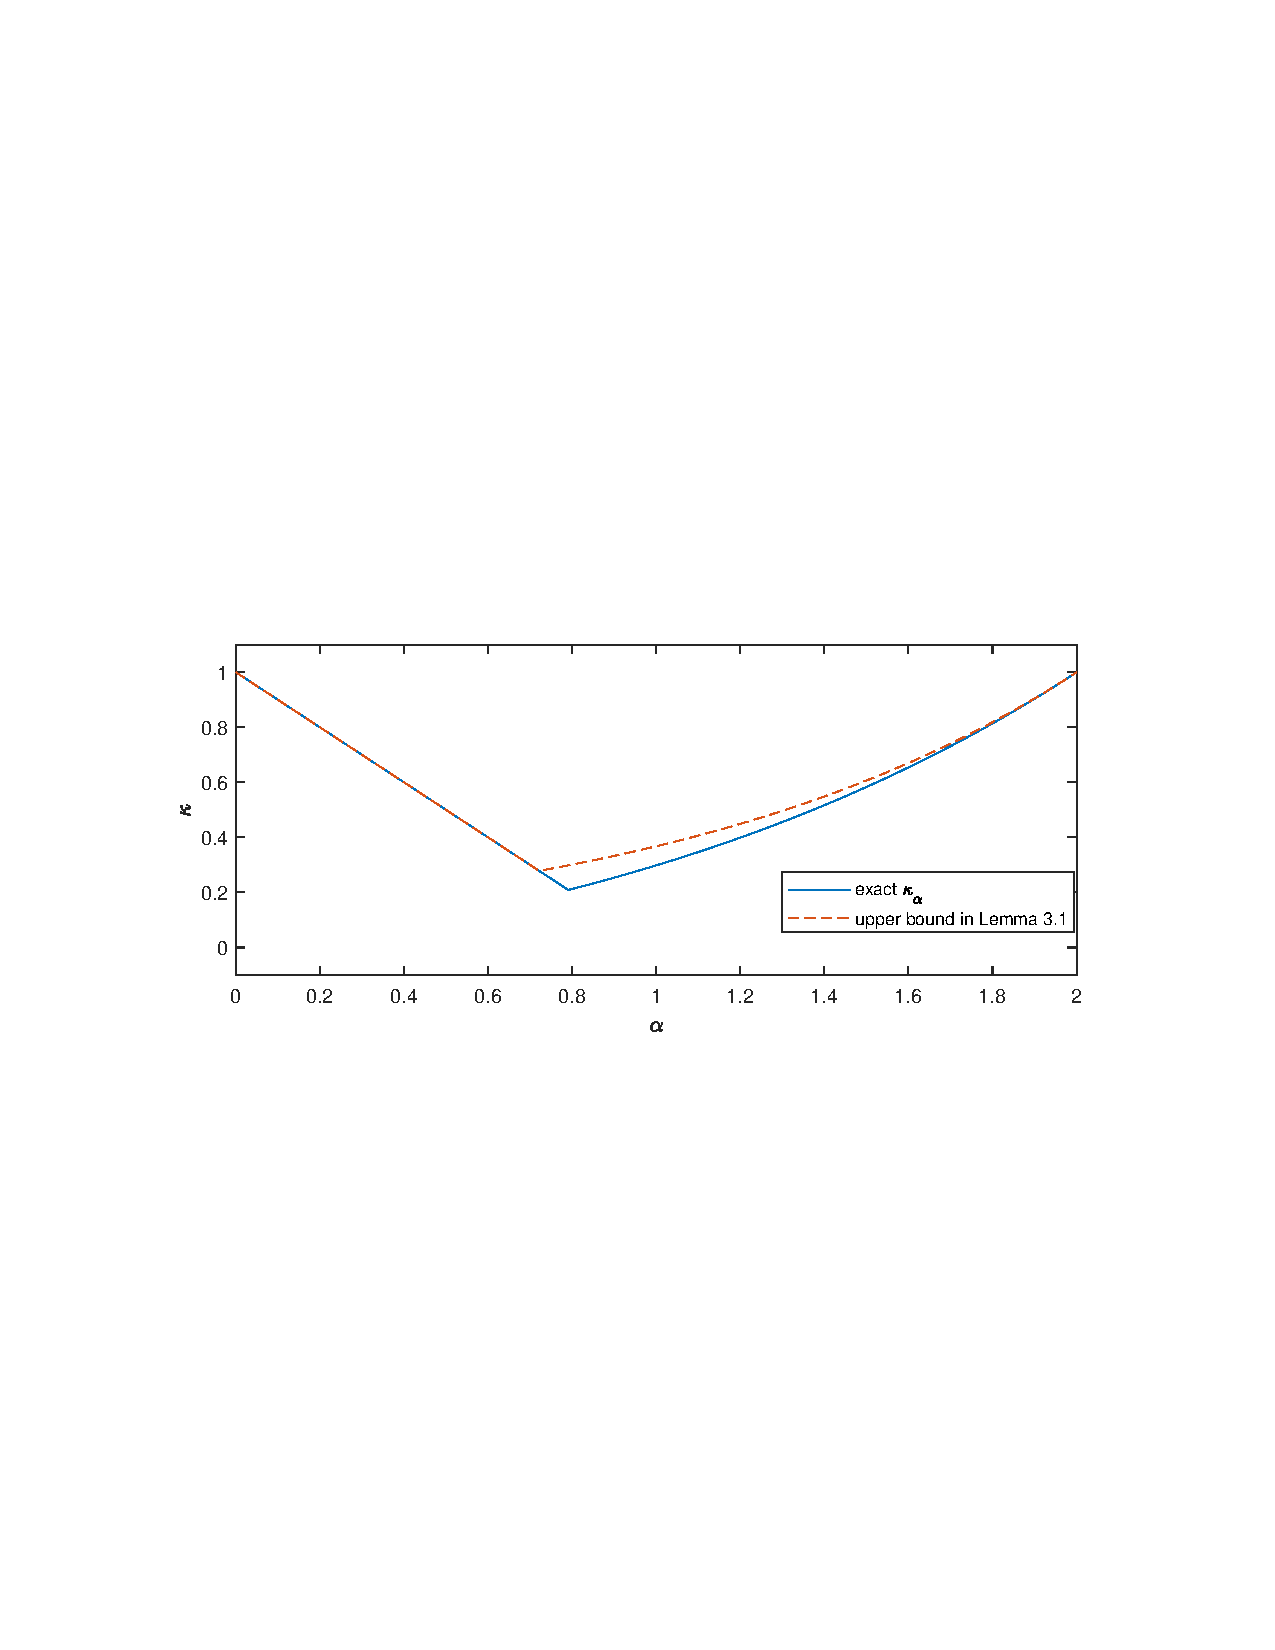
\includegraphics[width=0.6\textwidth]{kappa.pdf}
   \caption{Plot of $\kappa_\alpha$ defined in lemma \ref{lem:exp}.}
   \label{fig:ka-alpha}
\end{figure}


The next lemma provides a sharper estimate for $\kappa_1$.

%%
\begin{lemma}\label{lem:exp-1}
Let $\kappa_\alpha$ be the constant defined in \eqref{eqn:kappa-alpha}. Then $\kappa_1\approx 0.2984$.
\end{lemma}

\begin{proof}
To show the sharp estimate, we note that for $g(s) = 1-(1+s)e^{- s}$, there holds
$g'(s) = se^{-s} \ge 0$ and $g(0) = 1$. Therefore $g(s)\ge0$ for all $s\in(0,\infty)$.
This further implies $\psi(s)=(1-(1+s)e^{- s})/s \ge 0$ for $s\in (0,\infty)$.

Meanwhile, we note that
$$\varphi(s) := s^2 e^s \psi'(s) =  s^2 +s+1 -e^s. $$
{By checking the monotonicity, it is easy to verify that $\varphi(s)$ has a unique root, denoted by $s_*$, in $(0,\infty)$.
It further implies the function $\psi(s)$ achieves its maximum at $s^*$, i.e., $\kappa_1 = \psi(s_*)$.
Finally, the fixed-point iteration $s_{k+1} = \ln(s_k^2+s_k+1)$ and the contraction mapping theorem for $s\in[1.5,2]$ provide $s^*\approx1.793$, and hence $\kappa_1\approx 0.2984$.}
\end{proof}



Now we state our main theorem which verifies the desired result \eqref{eqn:conv-factor} with $\gamma\approx 0.3$.


% \begin{theorem}\label{thm:r}

% For a real function $r(x)$ satisfying that
% \begin{itemize}
%     \item $r(0) = 1$;
%     \item $r'(0) = -1$;
%     \item $|r(x)\leq(1+cx)^{-1}$, for some $c\in(0,1]$.
% \end{itemize}

% $R^\J(x) = r(x/\J)^\J$. Then
% $$\lim_{\J\to\infty}\sup_{x>0}\left|\frac{(1+x)R^\J(x)-1}{x}\right|\leq \max\{\kappa_1, \kappa_c\}.$$

% Proof:
% Since $r(0) =1, r'(0) = -1$, then for arbitary $\alpha > 1$, $\exists \delta >0$,
% s.t. $\forall 0\leq x\leq \delta$, $e^{-\alpha x}\leq r(x)$.

% For $0 < x \leq \J\delta$, $e^{-\alpha x}\leq R^\J(x) \leq (1+cx/\J)^{-\J}$.

% Therefore
% $$\lim_{\J\to\infty}\sup_{0\leq x \leq \J\delta}
% \left| \frac{(1+x)R^\J(x)-1}{x}  \right| \leq \max\{\kappa_\alpha, \kappa_c\}.$$

% For $x\geq \J\delta$,

% $\begin{aligned}
%     &\left|\dfrac{(1+x)R^\J(x)-1}{x}\right| \leq \frac{1+x}{x} |R^\J(x)| + \frac1x\\
%     &\leq C(\delta) (1+cx/\J)^{-\J}+(\J\delta)^{-1}\\
%     &\leq C(\delta)(1+c\delta)^{-\J}+(\J\delta)^{-1} \to 0
%     \mbox{~uniformly when~} \J \to 0.
% \end{aligned}$

% Therefore
% $$\lim_{\J\to\infty}\sup_{x\geq 0}
% \left| \frac{(1+x)R^\J(x)-1}{x}  \right| \leq \max\{\kappa_\alpha, \kappa_c\}.$$

% Since $\alpha$ is arbitary, and $\kappa_\alpha$ is continuous with $\alpha$,
% we can know that
% $$\lim_{\J\to\infty}\sup_{x>0}\left|\frac{(1+x)R^\J(x)-1}{x}\right|\leq \max\{\kappa_1, \kappa_c\}.$$
% \qed

% \end{theorem}
%
%\begin{lemma}\label{lem:frac}
%For a given $\alpha \in[0, 2]$, define $r_\alpha(s) = (1+\alpha s)^{-1}$.
%%and   $R_\alpha^\J(x) = r_\alpha(x/\J)^J$.
%Then there holds
%$$ \lim_{J\rightarrow\infty}\sup_{s\geq0}\left|\frac{(1+s)(1+\alpha s/J)^{-J}(s)-1}{s}\right|=\kappa_\alpha.$$
%\end{lemma}
%
%\begin{proof}
%It suffices to show that
%$$\lim_{J\rightarrow\infty}\sup_{s\geq0}\frac{(1+s)}{s} \left|(1+\alpha s/J)^{-J}-e^{-\alpha s}\right|=0.$$
%Then this and Lemma \ref{lem:exp} leads to the desired result.
%
%For a given $\delta>0$, for any $s>\delta$,  it is obvious that $(1+s)/s$
%is bounded by a constant $C(\delta)$. Meanwhile, we have the estimate \cite[Lemma A.1]{JinLazarovThomeeZhou:2017}
%\begin{equation*}
%\left|(1+\alpha s/J)^{-J}-e^{-\alpha s}\right| \le c J^{-1}.
%\end{equation*}
%Then we derive
%\begin{equation*}
%\lim_{J\rightarrow\infty}\sup_{s> \delta}\frac{(1+s)}{s} \left|(1+\alpha s/J)^{-J}-e^{-\alpha s}\right|=0.
%\end{equation*}
%
%For $0 < s \leq\delta$, we can show that
%\begin{equation*}
%\begin{aligned}
%   &\quad \frac{(1+s)}{s}   \left|(1+\alpha s/J)^{-J}-e^{-\alpha s}\right| \\
%  %  \leq \dfrac{(1+x)}{x} \left|(1+\alpha x / J)^{-J}-e^{\alpha x}\right| \\
%    &= \dfrac{(1+s)}{s}|(1+\alpha x / J)^{-1}-e^{-\alpha s/J}|
%    \left|\sum_{i=0}^{J-1} (1+\alpha x / J)^{-i} e^{ -(J-1-i)\alpha s/J}\right| \\
%    &\leq \dfrac{(1+s)}{s} \cdot C(\alpha, \delta)\Big(\frac{s}{J}\Big)^2 \cdot J \\
%    &\leq C(\alpha, \delta) J^{-1}.
%\end{aligned}
%\end{equation*}
%Here we use the fact that for $ s\in (0,\delta]$
%$$|(1+\alpha s / J)^{-1}-e^{-\alpha s/J}| \le C(\alpha, \delta)\Big(\frac{s}{J}\Big)^2 ~~\text{and}~~
%\max_{0\le i\le J-1}\left|(1+\alpha s / J)^{-i} e^{ (J-1-i)\alpha s/J} \right| \le C(\alpha, \delta)$$
%Therefore we arrive at
%$$\lim_{\J\to\infty}\sup_{0<s\leq\delta}\frac{(1+s)}{s} \left|(1+\alpha s/J)^{-J} -e^{-\alpha s}\right|=0.$$
%which completes the proof of the lemma.
%\end{proof}


\begin{theorem}\label{thm:conv-1}
Let conditions (P1)-(P3) hold valid. Then there exists a threshold $J_*>0$ such that
for all $J\ge J_*$
 \begin{equation*}
\sup_{s\in(0,\infty)}  \left|\frac{(1+s) r(-s/J)^J-1}{s}\right| \le 0.3,
\end{equation*}
        \end{theorem}
\begin{proof}
First of all, we aim to show that
 \begin{equation}\label{eqn:lim}
  \lim_{J\rightarrow\infty}\sup_{s\geq0}\frac{(1+s)}{s} \left|r(-s/J)^J-e^{- s}\right|=0.
  \end{equation}
For a given $\delta>0$, for any $s>\delta$,  it is obvious that $(1+s)/s$
is bounded by a constant $C(\delta)$. Meanwhile, note that
conditions (P1)-(P3) are fullfilled.
Then by means of the nonsmooth data error estimate \cite[Theorem 7.2]{Thomee:2006}, there holds
\begin{equation*}
\left|r(-s/J)^J-e^{-  s}\right| \le c J^{-q},
\end{equation*}
where $c$ is independent of $s$.
Then we derive
\begin{equation*}
\lim_{J\rightarrow\infty}\sup_{s> \delta}\frac{(1+s)}{s} \left|r(-s/J)^J-e^{-  s}\right|=0.
\end{equation*}
For $0 < s \leq\delta$, conditions (P1) and (P2) imply
\begin{equation*}
\begin{aligned}
   &\quad \frac{(1+s)}{s}   \left|r(-s/J)^J-e^{-  s}\right| \\
  %  \leq \dfrac{(1+x)}{x} \left|(1+\alpha x / J)^{-J}-e^{\alpha x}\right| \\
    &= \dfrac{(1+s)}{s}|r(-s/J)-e^{- s/J}|
    \left|\sum_{i=0}^{J-1} r(-s/J)^{i} e^{ -(J-1-i)  s/J}\right| \\
    &\leq \dfrac{(1+s)}{s} \cdot C(\alpha, \delta)\Big(\frac{s}{J}\Big)^{q+1} \cdot J \\
    &\leq C(\alpha, \delta) J^{-q}.
\end{aligned}
\end{equation*}
%Here we use the fact that for $ s\in (0,\delta]$
%$$|(1+\alpha s / J)^{-1}-e^{-\alpha s/J}| \le C(\alpha, \delta)\Big(\frac{s}{J}\Big)^2 ~~\text{and}~~
%\max_{0\le i\le J-1}\left|(1+\alpha s / J)^{-i} e^{ (J-1-i)\alpha s/J} \right| \le C(\alpha, \delta)$$
Therefore we arrive at
$$\lim_{J\to\infty}\sup_{0<s\leq\delta}\frac{(1+s)}{s} \left|r(-s/J)^{J} -e^{- s}\right|=0,$$
which completes the proof of the \eqref{eqn:lim}.
This together with Lemma \ref{lem:exp-1} implies that
    $$\lim_{J\to\infty}\sup_{s\in(0,\infty)}
    \left| \frac{(1+s)r(-s/J)^J-1}{s}  \right| = \kappa_1 < 0.3,$$
which completes the proof of the lemma.
\end{proof}

Next, using Theorem \ref{thm:conv-1}, we are able to show the linear convergence of the parareal iteration \ref{alg:para}.

\begin{theorem}\label{thm:conv-2}
Let conditions (P1)-(P3) be fullfilled and the data regularity in Lemma \ref{lem:conv-00} hold valid. Let $u^n$ be the solution to the time stepping scheme \eqref{eqn:semi},
and $U_k^n$ be the solution obtained from the parareal algorithm \ref{alg:para}.  Then there exists a threshold $J_*>0$ such that
for all $J\ge J_*$,
 we have
$$ \max_{1 \le n\le N_c} \| U_k^n - u^{nJ} \|  \le c \gamma^k\quad \text{with} \quad \gamma=0.3.$$
\end{theorem}

\begin{proof}
In Algorithm \ref{alg:para}, the initial guess $U_0^n$ is obtained by the coarse propagator, i.e., the backward Euler scheme.
Then Lemma \ref{lem:conv-00} (with $q=1$) implies the estimate
\begin{equation}\label{eqn:conv-3}
\begin{aligned}
 \| U_0^n - u^{nJ} \| &\le \| U_0^n - u(T^n)\|  + \|u(T^n)- u^{nJ} \| \\
 &\le c \big((\Delta T) {(T^n)}^{-1} + (\Delta t) {(t^{nJ})}^{-1} \big)\le c n^{-1}.
\end{aligned}
\end{equation}
Let $E_k^n =U_k^n - u^{nJ}$ and $e_{k,j}^n = (E_k^n, \phi_j)$. The the relation \eqref{eqn:factor-0} and
Theorem \ref{thm:conv-1} imply
\begin{equation*}
\begin{aligned}
\sup_{1\le n\le N_c} \|  E_k^n \|^2
& \le  \sum_{j=1}^\infty \sup_{1\le n\le N_c} | e_{k,j}^n |^2 \le \gamma^2  \sum_{j=1}^\infty \sup_{1\le n\le N_c} | e_{k-1,j}^n |^2\\
& \le \cdots     \le \gamma^{2k}  \sum_{j=1}^\infty \sup_{1\le n\le N_c} | e_{0,j}^n |^2
    \end{aligned}
\end{equation*}
with $\gamma = 0.3$. This together with the estimate
$
  \sup_{1\le n\le N_c} | e_{0,j}^n |^2 %\le  \frac{c}{\Delta T^{\frac12}} \Big(\Delta T\sum_{n=1}^{N_c} | e_{0,j}^n |^2\Big)^{\frac12}
   \le  \sum_{n=1}^{N_c} | e_{0,j}^n |^2
$
leads to
\begin{equation*}
\begin{aligned}
\sup_{1\le n\le N_c} \|  E_k^n \|^2  &\le c \gamma^{2k}  \sum_{j=1}^\infty  \sum_{n=1}^{N_c} | e_{0,j}^n |^2
 \le  c \gamma^{2k}   \sum_{n=1}^{N_c} \| E_{0}^n \|^2
  \le  c \gamma^{2k}   \sum_{n=1}^{N_c} n^{-2}
 \le c \gamma^{2k} ,
    \end{aligned}
\end{equation*}
where in the second last inequality we apply the estimate \eqref{eqn:conv-3}.
 This completes the proof of the theorem.
\end{proof}


\begin{remark}\label{rem:conv-1}
Theorem \ref{thm:conv-2} provides an useful upper bound of the convergence factor for all single step integrators
(satisfying (P1)-(P3)),
which might not be sharp for specific one. For example, in \cite[Lemma 4.3]{MathewSarkisSchaerer:2010},
Mathew, Sarkis and Schaerer considered the backward Euler method and proved
that the convergence factor of the Parareal algorithm is around $0.298$ (with $J_*=2$).
In \cite{Wu:2015}, Wu showed that convergence factors are $0.316$ (with $J_*=2$) and $0.333$ (with $J_*=2$)
for the second-order diagonal implicit Runge--Kutta method
and a single step TR/BDF2 method (i.e., the ode23tb solver for ODEs in MATLAB), respectively.
These error bounds might be slightly improved by increasing $J_*$.
See also \cite{WuZhou:2015} for the analysis for a third-order diagonal implicit Runge--Kutta method with a convergence factor $0.333$ and $J_*=4$.
\end{remark}


\begin{remark}\label{rem:conv-2}
Theorem \ref{thm:conv-2} only provides the existence of the threshold $J_*$ without any upper bound estimate.
It is obvious that a huge $J_*$ may destroy the parallelism of the algorithm.
Then a question arise naturally: is it possible to find $J_*$ for a given scheme satisfying conditions (P1)-(P3)? This is the focus of Section \ref{sec:RK}.
\end{remark}


\section{Case Studies for Several High-Order Single-Step Integrators}\label{sec:RK}

In this section, we shall study some popular single step methods. As we mentioned in Remark \ref{rem:conv-2},
Theorem \ref{thm:conv-2} did not provide a sharp estimate for the threshold $J_*$.
In fact, there is no universal estimate for all single step methods. Fortunately,
for any given single step integrator satisfying conditions (P1)-(P3) and fixed convergence rate
$\gamma>0.2984$,
we have a regular routine to find a sharper estimate for $J_*$.


We consider three time-stepping methods,
namely the the two-, three-, four-stage Lobatto IIIC methods, which are respectively second-, fourth- and sixth-order accurate, to the
initial and boundary value problem \eqref{eqn:pde}.
For the reader's convenience, we present the Butcher tableaus of the
two-, three-, four-stage Lobatto IIIC methods, respectively,
 %described by the Butcher tableau
%
\begin{equation}
\label{2-stage}
\begin{tabular}{cc|c}
 $\frac12$ &  $-\frac12$  & $0$\\[2pt]
 $\frac12$  & $\frac12 $& $1$ \\[2pt]
\hline
 $\frac12 $  & $\frac12$  & $\; $ \\
\end{tabular}
\ =:
\begin{tabular}{c|c}
 $\AA$ & $c$ \\[1pt]
\hline
 $b^\top$  & $\vphantom{\sum^{\sum^\sum}} $ \\
\end{tabular}
\end{equation},

\begin{equation}
\label{3-stage}
\begin{tabular}{ccc|c}
 $\frac16$ &  $-\frac31$
 & $\frac16$ & $0$ \\[2pt]
 $\frac16$  & $\frac5{12}$
 & $-\frac1{12}$ & $\frac12$ \\[2pt]
 $\frac16$  & $\frac23$
 & $\frac16$ & $1$ \\*[3pt]
\hline
 $\frac16 $  & $\frac23$ & $ \frac16$   & $\; $ \\
\end{tabular}
\ =:
\begin{tabular}{c|c}
 $\AA$ & $c$ \\[1pt]
\hline
 $b^\top$  & $\vphantom{\sum^{\sum^\sum}} $ \\
\end{tabular}
\end{equation}
%
and
%
\begin{equation}
\label{4-stage}
\begin{tabular}{cccc|c}
 $\frac1{12}$ &  $-\frac {\sqrt{5}}{12}$
 & $\frac {\sqrt{5}}{12}$ & $-\frac1{12}$ & $0$ \\*[2pt]
 $\frac1{12}$  & $\frac14 $ & $\frac{10-7\sqrt{5}}{60}$
 & $\frac{\sqrt{5}}{60}$
 & $\frac12-\frac{\sqrt{5}}{10}$\\*[2pt]
 $\frac1{12}$  & $\frac{10+7\sqrt{5}}{60}$
 &$\frac14$& $-\frac{\sqrt{5}}{60}$
 &  $\frac12+\frac{\sqrt{5}}{10}$ \\*[2pt]
  $\frac1{12}$ & $\frac5{12}$ &  $\frac5{12}$
 & $\frac1{12}$ & $1$ \\[3pt]
\hline
   $\frac1{12}$ & $\frac5{12}$ &  $\frac5{12}$
 & $\frac1{12}$ &  \\
\end{tabular}
\ =:
\begin{tabular}{c|c}
 $\AA$ & $c$ \\[1pt]
\hline
 $b^\top$  & $\vphantom{\sum^{\sum^\sum}} $ \\
\end{tabular}
\,.
\end{equation}
%

Let us also briefly recall some  well-known facts about Lobatto IIIC; for details we refer to \cite{HairerWanner:2010}.

These methods can be viewed as discontinuous collocation methods.
%The \textsl{stage order} of their $q$-stage members is $q-1$.
The \textsl{order} of the $m$-stage Lobatto IIIC methods is
$q=2m-2$.
In particular, the methods are \textsl{algebraically stable} and
{\textsl{L-stable}}, that makes them suitable for stiff problems.
The stability functions $r$,
%
\[r(z):=1+z b^\top (I-z\AA)^{-1} \mathbbm{1}\quad\text{with}\quad  \mathbbm{1}:=(1,\dotsc,1)^\top\in \R^q,\]
%
is given by the $(m-2,m)$-Pad\'e
approximation to $e^z$ and
vanishes at infinity, i.e., $r(\infty)=1-b^T \AA^{-1} \mathbbm{1}=0.$
Note that the computational cost of implicit Runge-Kutta methods increases fast with the stage number, and we refer
to \cite{Butcher:1976, RK:1988, JN:1995} and the reference therein for some efficient implementations.

The following argument highly depends on the upper bound for the constant $\kappa_\alpha$
defined in \eqref{eqn:kappa-alpha}. From Figure \ref{fig:ka-alpha},
we observe that Lemma \ref{lem:exp} gives an sharp estimate
for $\kappa_\alpha$ for $\alpha<0.7$, while the estimate for $\alpha>1$ could be further improved. The next lemma provides an estimate for $\alpha=1.02$, which is useful in the analysis of convergence rate.

\begin{lemma}\label{lem:exp-102}
Let $\kappa_\alpha$ be the constant defined in \eqref{eqn:kappa-alpha}. Then $\kappa_{1.02} \approx 0.3078<0.31$.
\end{lemma}

\begin{proof}
With $\beta=1.02 \geq 1$ and $\psi(s) = \frac{(1+s)e^{-\beta s} - 1}{s}$,
we observe that
$\psi(0+) = 1-\beta$ and $\psi(\infty)= 0$.
Meanwhile, since $e^{-\beta s} \leq e^{-s} \leq (1+s)^{-1}$ for $s\ge0$,
we derive that $\psi(s) \leq 0$.
Now we intend to show that $\psi'(s)$ admits a unique root in $(0,\infty)$, denoted as $x_*$. Then $\kappa_{\beta} = \psi(x_*)$.
Noting that
$$\psi'(s) =
\frac{1-(1 + \beta s + \beta s^2)e^{-\beta s}}{s^2},$$
it suffices to show that
$g(s) = 1-(1 + \beta s + \beta s^2)e^{-\beta s}$ has a unique root in $(0,\infty)$.
It is straightforward to see that the function
$$g'(s) = (-2+\beta + \beta s)\beta s e^{-\beta s}$$
admits a unique root in $(0,\infty)$. Then by the fact that $g(0)=0$ and Rolle's theorem, we conclude that $g$ has at most one root in $(0,\infty)$.
Meanwhile, we observe $\psi'(1)=1-(1+2\beta)e^{-\beta} \approx -0.0962 <0$ and
$\psi'(2) = \frac{1-(1+6\beta)e^{-2\beta}}{4} \approx 0.01855 >0$.
Therefore, there exists a unique root of $\psi'$ in $(0, \infty)$, named as $x_*$,
which lies in $(1,2)$.
{Then the fixed-point iteration $s_{k+1} = \ln(\beta s_k^2+\beta s_k+1)/\beta$ and the contraction mapping theorem for $s\in[1.5,2]$ provide $s_*\approx 1.715$,
and hence $\kappa_\beta = f(x_*) \approx 0.3078 \le 0.31$.}
\end{proof}


\begin{proposition}\label{prop:lobatto-2}
Let $u^n$ be the solution to the time stepping scheme \eqref{eqn:semi} using
the two-stage Lobatto IIIC method \eqref{2-stage},
and $U_k^n$ be the solution obtained from the parareal algorithm \ref{alg:para}. Then for all $J\ge 2$, there holds
$$ \max_{1 \le n\le N_c} \| U_k^n - u^n \|  \le c \gamma^k\quad \text{with} \quad \gamma=0.31.$$
\end{proposition}

\begin{proof}
It suffices to show that for any $J\ge 2$, there holds
\begin{equation}\label{eqn:lobatto-2}
    \sup_{s\in(0,\infty)}  \left|\frac{(1+s) r(-s/J)^J-1}{s}\right| \le 0.31,
    \quad
    \text{where}~~ r(-s) = \frac{2}{s^2+2s+2}.
\end{equation}
To this end, we define $\alpha = 0.69$ and $\beta=1.02$.
Then Lemma \ref{lem:exp} implies that
$\kappa_\alpha \le 1-0.69 = 0.31$,
and meanwhile Lemma \ref{lem:exp-102} indicates $\kappa_\beta \le 0.31$.

Next, we aim to show that $e^{-\beta s} \le r(-s) \le e^{-\alpha s}$ for all $s\in(0,s_*)$ with $s_*=3.2$. First of all, using the fact that
$\frac{2}{s^2+2s+2} \ge {e^{-s}} \ge e^{-\beta s}$ for all $s > 0$, we derive
the first inequality $e^{-\beta s} \le r(-s)$.
Then we turn to the second inequality
$r(-s) \le e^{-\alpha s}$, equivalent to
$g(s) := 2e^{\alpha s} -(s^2+2s+2) \le 0$ in  $(0, s_*)$.
Noting that $g''(s) = 2\alpha^2 e^{\alpha s} - 2$, which admits a
unique root at $-\frac{2\ln \alpha}{\alpha}$.
Meanwhile, we observe that
$g''(s) <0$ in $(0, -\frac{2\ln \alpha}{\alpha})$,
and $g''(s) >0$ in $( -\frac{2\ln \alpha}{\alpha}, \infty)$.
Besides, since $g'\left( -\frac{2\ln \alpha}{\alpha}\right)  =
\frac{4\ln \alpha +2-2\alpha}{\alpha}<0$
and $g'(0)=2\alpha-2 <0$, we conclude that
$g'(s) < 0$ in $(0, -\frac{2\ln \alpha}{\alpha})$,
and $g'(s)$ has a unique root in $(-\frac{2\ln \alpha}{\alpha}, \infty)$. Moreover, the facts $g'(2) \approx -0.5 <0$ and $g'(3) \approx 2.9 >0$ implies that
there exists a constant $s_1 \in (2,3)$, s.t. $g'(s_1)= 0$,
and $g'(s) <0$ in $(0, s_1)$,
$g'(s) >0$ in $(s_1, \infty)$.
Then we note that $g(s_*) = -0.445 <0$ and conclude that
$g(s) := 2e^{\alpha s} -(s^2+2s+2) \le 0$ in  $(0, s_*)$,
which implies $r(s) \le e^{-\alpha s}$ in $(0, s_*)$.
As a result, we arrive at $e^{-\beta s} \le r(-s/J)^J \le e^{-\alpha s}$
for all $s\in(0, J s_*)$ which  implies
\begin{equation*}
    \sup_{s\in(0, J s_*)}
    \left|\frac{(1+s) r(-s/J)^J-1}{s}\right| \le 0.31.
\end{equation*}

Besides, we observe the fact that
$$\sup\limits_{(s_*, \infty)}
\Big|\frac{2}{s^2 + 2s + 2}\Big|
= \Big|\frac{2}{s_*^2 + 2s_* + 2}\Big|
\approx 0.1073 < 0.11.$$
Then we derive for $s\in (Js_*,\infty)$ and $J\ge 2$
\begin{equation*}
\begin{split}
    \left|\frac{(1+s) r(-s/J)^J-1}{s}\right|
    &\le \frac{1+s}{s}|r(-s/J)^J|+s^{-1}
    \le \frac{1+Js_*}{Js_*} (0.11)^J + (Js_*)^{-1}    \\
    &\le  \frac{1+6.4}{6.4} (0.11)^2 + (2\times 3.2)^{-1}
    \approx 0.1702 \le 0.31.
\end{split}
\end{equation*}
This completes the proof of \eqref{eqn:lobatto-2}.
\end{proof}

The argument could be further extended to the high-order time stepping scheme, e.g., 3- or 4-stage Lobatto IIIC method.
This result is given in the following proposition.

\begin{proposition}\label{prop:lobatto-34}
Let $u^n$ be the solution to the time stepping scheme
\eqref{eqn:semi} using
the three-stage Lobatto IIIC method \eqref{3-stage} or the four-stage Lobatto IIIC method \eqref{4-stage},
and $U_k^n$ be the solution obtained from the parareal algorithm \ref{alg:para}. Then for all $J \ge 2$, there holds
$$ \max_{1 \le n\le N_c} \| U_k^n - u^n \|  \le c \gamma^k\quad \text{with} \quad \gamma=0.31.$$
\end{proposition}

Proof for the 3-stage Lobatto IIIC scheme \eqref{3-stage}: 


Similar to the proof of proposition \ref{prop:lobatto-2}, we aim to show that for any $J\ge 2$
\begin{equation}\label{eqn:lobatto-3}
    \sup_{s\in(0,\infty)}  \left|\frac{(1+s) r(-s/J)^J-1}{s}\right| \le 0.31,
    \quad
    \text{where}~~ r(-s) = \frac{24-6s}{s^3 + 6s^2 + 18s + 24}.
\end{equation}
Letting $\alpha = 0.69$ and $\beta=1.02$,
Lemmas \ref{lem:exp} and \ref{lem:exp-102} implies that
$\kappa_\alpha \le 1-0.69 = 0.31$ and $\kappa_\beta \le 0.31$, respectively.

Next, we show the claim that $e^{-\beta s} \le r(-s) \le e^{-\alpha s}$ for all $s\in(0,s_*)$ with $s_*=2$. To begin with, we shall prove that $r(-s) > e^{-\beta s}$ for all $s\in(0,\infty)$, which is equivalent to
$$\psi(s) = e^{\beta s} (-6s+24) - (s^3+6s^2+18s+24) >0
\quad \forall ~s\in (0, s_*).$$
We note that
$$\psi^{(4)}(s) = 6\beta^3e^{\beta s}(-\beta s + 4\beta - 4).$$
has a unique root in $(0,\infty)$, namely
$s_0= \frac{4\beta - 4}{\beta} \approx0.0784$, and hence
$\psi^{(4)}(s)> 0$ for all $s\in(0,s_0)$.
Besides, we observe that
$\psi^{(3)}(0) = 0.742 >0$, $\psi^{(3)}(s_0) \approx 0.762 >0$.
Therefore $\psi^{(3)}(s)$ has a unique root
in $(s_0, +\infty)$,
denoted as $s_1$. By means of the fixed point iteration, we know that
$s_1\approx 0.4832$.
Similarly, since $\psi''(0) =  0.730>0$ and $\psi''(s_1) =  1.00>0$, we conclude that $\psi''(s)$ is always positive in $[0,s_1]$ and it
has a unique root $s_2\in (s_1,\infty)$, and we find $s_2\approx 0.9980$.
Repeating the argument, we are able to show that
$\psi'(s)$ keeps positive in $[0,s_2]$ and
the unique root in $(s_2,\infty)$ locates at
$s_3 \approx 1.5344$.
Finally, we observe that $\psi(0) = 0$ and $\psi(s_3) \approx 1.401>0$, so $\psi$ is positive in $(0,s_3]$
and it admits a unique root at $s_4\in(s_3,\infty)$.
Noting that $\psi(s_*) \approx 0.2873 > 0$,
we conclude that $r(-s) > e^{-\beta s}$ for all $s\in(0,s_0)$.

Next we will show that $r(-s) < e^{-\alpha s}$ in $(0, s_*)$, which is equivalent to show
\begin{equation*}
    \varphi(s) = e^{\alpha s} (-6s+24) - (s^3+6s^2+18s+24) < 0 \quad \text{for all} ~s\in (0, s_*).
\end{equation*}
We note the fact that
\begin{equation*}
\varphi^{(4)}(s) = 6\alpha^3e^{\alpha s}(-\alpha s + 4\alpha - 4)<0\quad \text{for all} ~s\in (0, \infty).
\end{equation*}
Meanwhile, we have $\varphi^{(4)}(0)<0$, $\varphi^{(3)}(0)<0$, $\varphi''(0)<0$, $\varphi'(0)<0$, and $\varphi(0)<0$.
Those together imply $\varphi(s) <0$ for any
$s\in (0, \infty)$. Therefore $r(-s) < e^{-\alpha s}$.

As a result, for any $J\ge 2$, we arrive at $e^{-\beta s} \le r(-s/J)^J \le e^{-\alpha s}$
for all $s\in(0, J s_*)$, that further implies the estimate
\begin{equation*}
    \sup_{s\in(0, J s_*)}
    \left|\frac{(1+s) r(-s/J)^J-1}{s}\right| \le 0.31.
\end{equation*}

Next, we aim to prove the claim that
\begin{equation}\label{claim:bound-3}
   \sup\limits_{(s_*, \infty)}
   \big|r(-s)\big| = \sup\limits_{(s_*, \infty)}
   \Big|\frac{24-6s}{s^3 + 6s^2 + 18s + 24}\Big|
   \le  0.15.
\end{equation}
To begin with, we show that $\frac{\d}{\d s}r(-s)$ admits a unique root in $(2, \infty)$. % ,  denoted as $s_5$.
We note that
$$\frac{\d}{\d s}r(-s) = \frac{12(s^3-3s^2-24s-48)}
{(s^3 + 6s^2 + 18s + 24)^2}.$$
and hence it is sufficient to show that
$\eta(s) = s^3-3s^2-24s-48$
has a unique root in $(2, \infty)$.
Since $\eta'(s)$ has two roots, $-2$ and $4$,
and $\eta(-2)=-20<0$, $\eta(4)=-128<0$,
we conclude that $\eta(s) <0$ for all $s\in[-2,4]$, and
$\eta(s)$ admits a unique root in $(4, \infty)$,
namely $s_5 \approx 7.235$. %7.234531027367
Therefore $r(-s)$ is decreasing in $(s_*,s_5)$
and increasing in $[s_5,\infty)$.
Noting that fact that $r(-s_*) \approx 0.130$,
$r(-s_5)\approx -0.0229$ and $r(-\infty)=0$, we obtian
$
    \sup\limits_{(s_*, \infty)}
    \big|r(-s)\big| = \big|r(-s_*)\big|
    \le  0.15.
$

Therefore, we derive for $s\in (Js_*,\infty)$ and $J\ge 2$
\begin{equation*}
\begin{split}
    \left|\frac{(1+s) r(-s/J)^J-1}{s}\right|
    &\le \frac{1+s}{s}|r(-s/J)^J|+s^{-1}
    \le \frac{1+Js_*}{Js_*} (0.15)^J + (Js_*)^{-1}    \\
    &\le  \frac{5}{4} (0.02)^2 + 4^{-1}
    \approx 0.251 \le 0.31.
\end{split}
\end{equation*}
This completes the proof of \eqref{eqn:lobatto-3} as well as the proposition.
\qed

Proof for the 4-stage Lobatto IIIC scheme \eqref{4-stage}:
Similar to the proof of Proposition \ref{prop:lobatto-2}, we aim to show that for any $J\ge 2$
\begin{equation}\label{eqn:lobatto-4}
    \sup_{s\in(0,\infty)}  \left|\frac{(1+s) r(-s/J)^J-1}{s}\right| \le 0.31,
    ~~
    \text{where}~~ r(-s) =
    \frac{12s^2-120s+360}{s^4+12s^3+72s^2 + 240s + 360}.
\end{equation}
Letting $\alpha = 0.69$ and $\beta=1.02$,
Lemmas \ref{lem:exp} and \ref{lem:exp-102} implies that
$\kappa_\alpha \le 1-0.69 = 0.31$ and $\kappa_\beta \le 0.31$, respectively. Next, we show the claim that
\begin{equation}\label{claim:sand}
    e^{-\beta s} \le r(-s) \le e^{-\alpha s}~~ \text{for all}~~s\in(0,s_*)~~ \text{with}~s_*=6.8.
\end{equation}

To begin with, we show that, for $s\in(0,\infty)$, $r(-s) \ge e^{-\beta s}$, which is equivalent to
$$\psi(s) = (12s^2-120s+360)e^{\beta s} -(s^4+12s^3+72s^2 + 240s + 360)
 \ge 0.$$
Define $h(s) = \beta^2s^2 + (10\beta-10\beta^2)s+(30\beta^2-50\beta+20)$,
then we have
$$\psi^{(5)}(s) = 12\beta^3e^{\beta s}
\left[\beta^2s^2 + (10\beta-10\beta^2)s+(30\beta^2-50\beta+20)\right]
=12\beta^3e^{\beta s}h(s).$$
Here $h(s)$ is a quadratic polynomial, whose
minimum locates at $\frac{5\beta-5}{\beta}$.
Therefore $h(s) \geq h (\tfrac{5\beta-5}{\beta} ) > 0$.
Then $\psi^{(5)}(s) = 12\beta^2e^{\beta x}h(s)-24 > 12\times 2-24>0$.
Meanwhile, simple computation yields
$$ \psi(0)=0 \qquad \text{and}
\qquad \psi^{(k)}(0)>0~~\quad \text{with}~~ \quad
1\le k\le 5.  $$
Then we conclude that  $\psi(s) > 0$ for all  $s\in (0, \infty)$, and hence
 $r(-s) \ge e^{-\beta s}$ in $(0, \infty)$.

Next we show the bound that $r(s) \le e^{-\alpha s}$ for $s\in (0,s_*)$, which is equivalent to show
$$\varphi(s) = (12s^2-120s+360)e^{\alpha s}
-(s^4+12s^3+72s^2 + 240s + 360) \le 0 \qquad \forall~s\in (0,s_*).$$
Similar to the preceding argument, let $g(s) = (20-50 \alpha + 30 \alpha^2  +10\alpha s -10\alpha^2s +\alpha^2s^2)$. Then
$$  \varphi^{(5)}(s) = 12\alpha^3e^{\alpha s}
(20-50 \alpha + 30 \alpha^2
+10\alpha s -10\alpha^2s +\alpha^2s^2)
= 12\alpha^3e^{\alpha s}  g(s). $$
Here $g$ is a quadratic polynomial with minimum at $\frac{5\alpha-5}{\alpha}$. Therefore, $g(s)\ge g(\tfrac{5\alpha-5}{\alpha}) \approx -2.62$.
Meanwhile, we observe that $g(0) = -0.217 <0$, so
there is a unique root of $g$ in $(0, \infty)$.
It is easy to find that, by means of the fixed point iteration,
that root locates at $s_0\approx0.0993$. Then $\varphi^{(5)}(s) \le 0$
for all $s\in [0,s_0]$ and $\varphi^{(5)}(s) \ge 0$ for $s\in (s_0,\infty)$. Noting that $\varphi^{(4)}(s_0) < 0$ and $\varphi^{(4)}(0) < 0$, so $\varphi^{(4)}(s) < 0$ in $[0,s_0]$ and $\varphi^{(4)}$ admits a unique root in $(s_0,\infty)$, named as $s_1$.
Then the fixed point iteration implies $s_1\approx  1.6849$.
Repeating this argument, we are able to show that
$\varphi^{(3)}(s) < 0$ in $[0,s_1]$ and $\varphi^{(3)}$ has a unique root $(s_1,\infty)$, namely $s_2\approx 3.0558$.
Then we derive that
$\varphi{''}(s) < 0$ in $[0,s_2]$ and  $\varphi{''}(s)$
has a unique root in $(s_2,\infty)$,
denoted as $s_3\approx 4.3640$.
Similarly, $\varphi{'}(s) < 0$ in $[0,s_3]$ and  $\varphi{'}(s)$
has a unique root in $(s_3,\infty)$, named as $s_4\approx 5.6285$.
Finally, since $\psi(0)=0$ and $\varphi(s_4)<0$, we conclude that
$\varphi(s)<0$ in $(0,s_4]$, and $\varphi(s)$ has a unique root in $(s_4,\infty)$. Then the fact that $\varphi(s_*) \approx -447.65<0$ implies $\varphi(s)<0$ in $(0,s_*)$.
This completes the proof of the claim \eqref{claim:sand}.
As a result, for any $J\ge 2$, we arrive at $e^{-\beta s} \le r(-s/J)^J \le e^{-\alpha s}$
for all $s\in(0, J s_*)$ which  implies
\begin{equation*}
    \sup_{s\in(0, J s_*)}
    \left|\frac{(1+s) r(-s/J)^J-1}{s}\right| \le 0.31.
\end{equation*}

Next, we intend to show the claim that
\begin{equation}\label{claim:bound-4}
 \sup\limits_{(s_*, \infty)}
   \big|r(-s)\big| =   \sup\limits_{(s_*, \infty)}  \big|\frac{12s^2-120s+360}{s^4+12s^3+72s^2 + 240s + 360}\Big| \le  0.02.
\end{equation}
In order to establish a bound for the supremum, we note
$$\frac{d}{ds}r(-s)
= \frac{-24s^5+216s^4+1440s^3-1440s^2-43200s-129600}
{(s^4+12s^3+72s^2 + 240s + 360)^2}, $$
and we will show that it admits a unique root in $(s_*, \infty)$,
denoted by $s_5$. Noting that, with
$\mu(s) = -s^5+9s^4+60s^3-60s^2-1800s-5400, $
we have
$$\frac{d}{ds}r(-s) = \frac{24\mu(s)}{(s^4+12s^3+72s^2 + 240s + 360)^2}.$$
So it suffices to show that $\mu(s)$ admits a unique  root in $(s_*, \infty)$. Since
$\mu^{(3)}(s)=-60s^2+216s+360,$ being a quadratic polynomial,
it gains the maximum at $1.8$ where
$\mu^{(3)}(1.8) = 554.4>0$.
Noting that $s_*>1.8$ and $\mu^{(3)}(s_*)=-945.6<0$,
we conclude that $\mu^{(3)}(s)<0$ for all $s\in(s_*, \infty)$.
Moreover, since $\mu''(s_*) \approx 1033.3 >0$ and $\mu''(\infty) =-\infty$, $\mu''(s)$ admits a unique root $s_6\approx 7.6503 \in (s_*, \infty)$. Then we know that $\mu''(s) > 0$ in $(s_*, s_6)$
and $\mu''(s) < 0$ in $(s_6, \infty)$.
Similarly, we have $\mu'(s_*) >0$ and $\mu'(s_6) >0$,
so  $\mu'(s) > 0$ in $[s_*, s_6]$. This together with the fact  $\mu'(\infty) <0$ implies that
$\mu'(s)$ has a unique root $s_7\approx 10.166 \in (s_6, \infty)$.
Finally, using the facts that $\mu(s_*)>0$ and $\mu(s_7)>0$,
we know $\mu(s) >0 $ in  $(s_*, s_7)$ and
 $\mu(s)$ has a unique root $s_8 \approx 12.28 \in (s_7, \infty)$.
Therefore $r(-s)$ is increasing in $(s_*, s_8)$,
and decreasing in $(s_8, \infty)$.
Noting that $r(-s)\approx 0.0088$, $r(-s_8)\approx 0.0118$, and $r(-\infty)=0$, we arrive at
$\sup\limits_{(s_*, \infty)}
\big|r(-s)\big| \le 0.02.$


As a result, the estimate \eqref{claim:bound-4} implies that
for $s\in (Js_*,\infty)$ and $J\ge 2$
\begin{equation*}
\begin{split}
    \left|\frac{(1+s) r(-s/J)^J-1}{s}\right|
    &\le \frac{1+s}{s}|r(-s/J)^J|+s^{-1}
    \le \frac{1+Js_*}{Js_*} (0.02)^J + (Js_*)^{-1}    \\
    &\le  \frac{14.6}{13.6} (0.02)^2 + 13.6^{-1}
    \approx 0.074 \le 0.31.
\end{split}
\end{equation*}
This completes the proof of \eqref{eqn:lobatto-4} as well as the proposition.
\qed


\begin{remark}
Propositions \ref{prop:lobatto-2} and \ref{prop:lobatto-34} show that, for two-, three-, four-stage Lobbatto IIIC schemes, the convergence factor is (at worst) $0.31$,
and there is no restriction
on the ratio between the coarse time step and fine
time step.
It is still possible to improve those estimations, by means of Theorem \ref{thm:conv-1}.
For example, one may obtain a smaller
convergence factor $\gamma$ by choosing a bigger $\alpha$ and
a smaller $\beta$, which might not affect the threshold $J_*=2$.
\end{remark}

\begin{remark}\label{rem:calahan}
In the proof of Propositions \ref{prop:lobatto-2} and \ref{prop:lobatto-34}, we employ the \textsl{L-stability} ($r(-\infty) = 0$) of the two-, three-, four-stage Lobbatto IIIC schemes. If the $r(-\infty) \in (0,1)$,
the analysis might be more technical, and the convergence might be
slow for small step ratio $J$; see e.g. Figure \ref{fig:ex1-b} for the Calahan scheme \eqref{eqn:Calahan}--\eqref{eqn:Calahan-p}.
However, Theorem \ref{thm:conv-1} guarantees the existence of the
threshold $J_*$ such that for any $J\ge J_*$ the convergence factor is close to $0.3$.
\end{remark}

{
\begin{remark}
The previous analysis shows that different $J$ lead to almost the same convergence rate. For a smaller $J$, or more corase intervals, the algorithm will be guaranteed a higher parallel ability and takes less CPU time if we have plenty CPU cores. 
\end{remark}}

\section{Numerical Results}\label{sec:parareal-numerical}
In this section, we shall present some numerical examples to illustrate and complement our theoretical results.
To begin with, we use the one-dimensional diffusion models to show the sharpness of our convergence analysis in Sections \ref{sec:convergence-parareal} and \ref{sec:RK}.

\paragraph{Example 1. Linear Diffusion Models}
We consider the following initial-boundary value problem of parabolic equations
\begin{equation}\label{eqn:diffusion}
    \left \{
\begin{aligned}
&\partial_t u (x,t) - \partial_{xx} u(x,t) = f(x,t), &&\quad 0<t<T,\\
& u(x,t)=0,&&\quad x\in\partial\Omega,~0<t<T, \\
& u(x,0)=u^0(x),&&\quad x\in\Omega.
\end{aligned}
\right.
\end{equation}
where $\Omega=(0,\pi)$ and $T=1$. We consider the following two sets of problem data
\begin{itemize}
    \item[(a)] $u^0(x) = x^{5}(1-x)^{5}/(\pi/2)^{10}$
    and $f\equiv0$;
    \item[(b)] $u^0(x) = \chi_{(0,\frac\pi2)}(x)$ and $f=\cos(t) \sin(x)$, where $\chi_{(0,\frac\pi2)}(x)$ denotes the step function:
    \begin{equation*}
 \chi_{(0,\pi/2)}(x)  =
 \begin{cases}
 1, \quad x\in(0,\pi/2),\\
0, \quad \text{elsewise}.
 \end{cases}
\end{equation*}
\end{itemize}

In the computation, we divided the domain $\Omega$ into with $M$ equal subintervals of length $h=\pi/M$ and apply the Galerkin finite element with piesewise linear polynomials to discretize in space.
We examine the error between the parareal iterative solution $U_k^n$ and the exact time stepping solution $U^n$, i.e.,
{$$ \text{error} = \max_{1\le n\le N_c}  \| U_k^n - u^{nJ} \|_{L^2(\Omega)} .  $$}
In our computation, we fixed
spatial mesh size $h=\pi/1000$, and choose the initial guess
$U_0^n = u^0$ for all $n=0,\ldots,N$.

In example (a), the data is sufficiently smooth and compatible to the homogeneous Dirichlet boundary condition. In fact, it is easy to show show that $u^0 \in \text{Dom}((-\Delta)^{3+\epsilon})$ with $\epsilon\in(0,1/4)$  (see e.g. Lemma \cite[Lemma 3.1]{Thomee:2006}). For this case of regular data, Bal showed that the first several parareal iterations converge linearly with the rate $O(\Delta T)$; see cf. \cite{Bal:2005}. This is fully supported by the numerical results presented in Figure \ref{fig:ex1-a}, where we show the convergence of parareal algorithm for $2$- and $3$-stage Lobatto IIIC methods with
fixed $J=10$ and $\Delta T = 1/100$, $1/300$, $1/600$ (and correspondingly $\Delta t = 1/1000$, $1/3000$, $1/6000$).
We observe that the convergence of the first several iterations is faster for smaller coarse step size,
but the convergence then deteriorates for the later iterations.

\begin{figure} [tbhp]
\centering
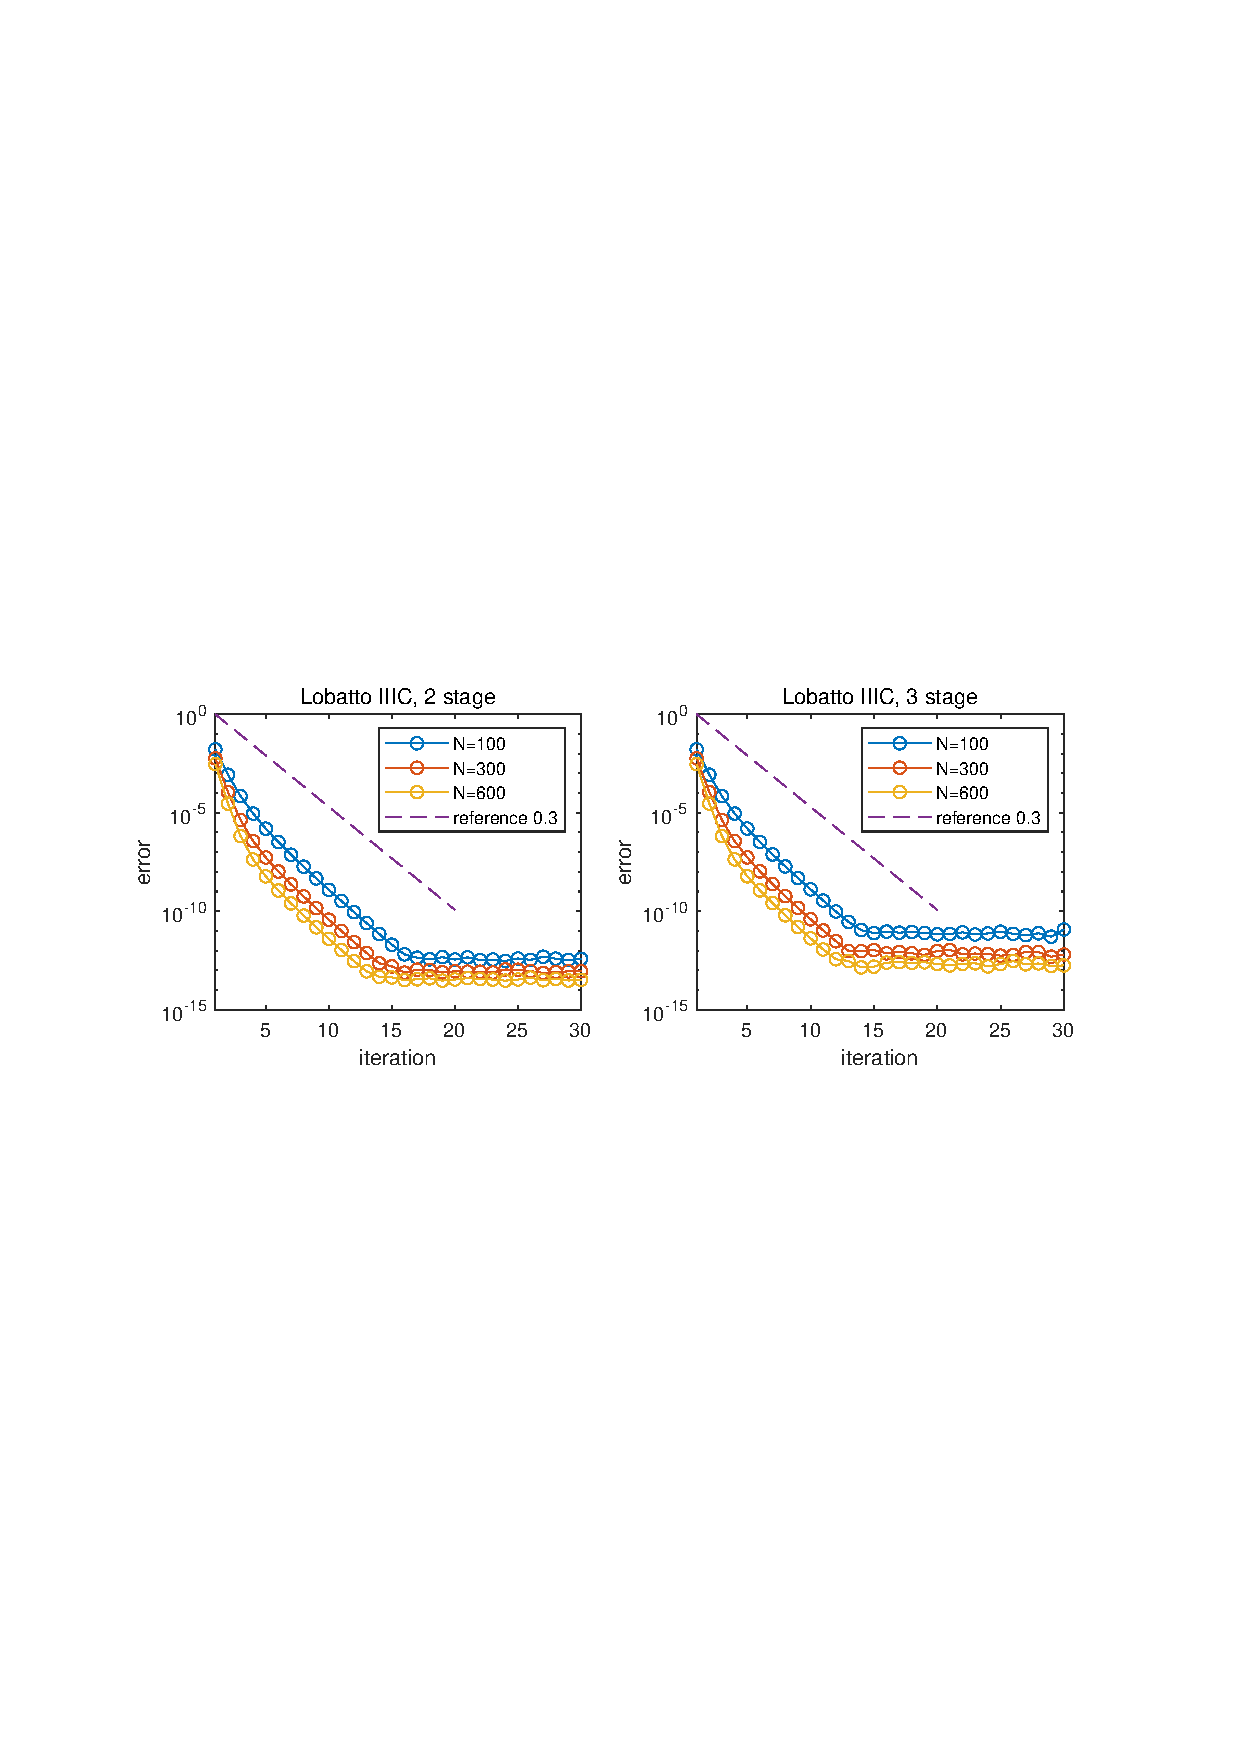
\includegraphics[width=1\textwidth]{fig102c.pdf}
\vskip-5pt   \caption{Example 1 (a): smooth data. Convergence of the parareal algorithm for $2$- and $3$-stage Lobatto IIIC methods with fixed mesh ratio $J=10$ and various coarse step sizes $1/N$, $N=100$, $300$, $600$.}
   \label{fig:ex1-a}
\end{figure}

In Figure \ref{fig:ex1-b}, we show the convergence of parareal algorithm for $2$-, $3$-, $4$-stage Lobatto IIIC methods solving
parabolic equation with nonsmooth initial data, i.e. Example 1 (b).
We fixed the fine step size $\Delta t = 1/3000$ and use different step ratios $J=2$, $3$ and $10$.
The numerical experiments clearly show that the parareal iterations converge linearly with convergence factor near $0.3$
for all $J\ge 2$. Meanwhile,
we observe that the convergence factor is independent of the ratio between coarse and find step sizes.
These phenomenon fully support our theoretical findings in  Propositions \ref{prop:lobatto-2} and \ref{prop:lobatto-34}.
Moreover, we test another time integrator,
called Calahan scheme \cite[eq. (1.9)]{Zlama:1974}, defined by
\begin{equation}\label{eqn:Calahan}
    r(-s) = 1-\frac{s}{1+bs} - \frac{\sqrt{3}}{6} \Big(\frac{s}{1+bs}  \Big)^2,\qquad \text{with}~~ b = \frac12\Big( 1 + \frac{\sqrt{3}}{3} \Big)
\end{equation}
and
\begin{equation}\label{eqn:Calahan-p}
\begin{aligned}
c_1 = \frac13,\qquad & p_1(-s) = \frac{(1/2 + \sqrt3) + (\sqrt3/2)s}{(1+bs)^2};\\
c_2 = \frac23,\qquad & p_2(-s) = \frac{(1/2 - \sqrt3) + (1/2 - \sqrt3/2)s}{(1+bs)^2}.
\end{aligned}
\end{equation}
The Butcher tableau is given by
\begin{equation}
\label{calahan}
\begin{tabular}{cc|c}
 $\frac16\sqrt{3}+\frac23$ &  $-\frac16\sqrt{3}-\frac13$  & $\frac13$\\[2pt]
 $-\frac16\sqrt{3}+\frac13$  & $\frac16\sqrt{3}+\frac13 $& $\frac23$ \\[2pt]
\hline
 $\frac12 $  & $\frac12$  & $\; $ \\
\end{tabular}
\ =:
\begin{tabular}{c|c}
 $\AA$ & $c$ \\[1pt]
\hline
 $b^\top$  & $\vphantom{\sum^{\sum^\sum}} $ \\
\end{tabular}
\end{equation}
It is easy to see that  $r(-s)$ is a decreasing function on $(0, \infty)$ and $r(-\infty)=1-\sqrt{3} \in (-1,0)$, so it is \textsl{A-stable}, but not \textsl{L-stable}.
Besides, the scheme is accurate of order $k=3$.
Therefore, the Calahan scheme satisfies Conditions (P1)--(P3).
Numerical results show that the converegnce of the corresponding parareal iterations is much slower than $0.3$ for small $J$.
This might be due to the fact that $|r(-\infty)| > 0$; see Remark \ref{rem:calahan}. However, for large $J$, the numerical results indicate a convergence rate close to $0.3$,
as predicted by Theorem \ref{thm:conv-2}.\vskip10pt



\begin{figure} [tbhp]
\centering
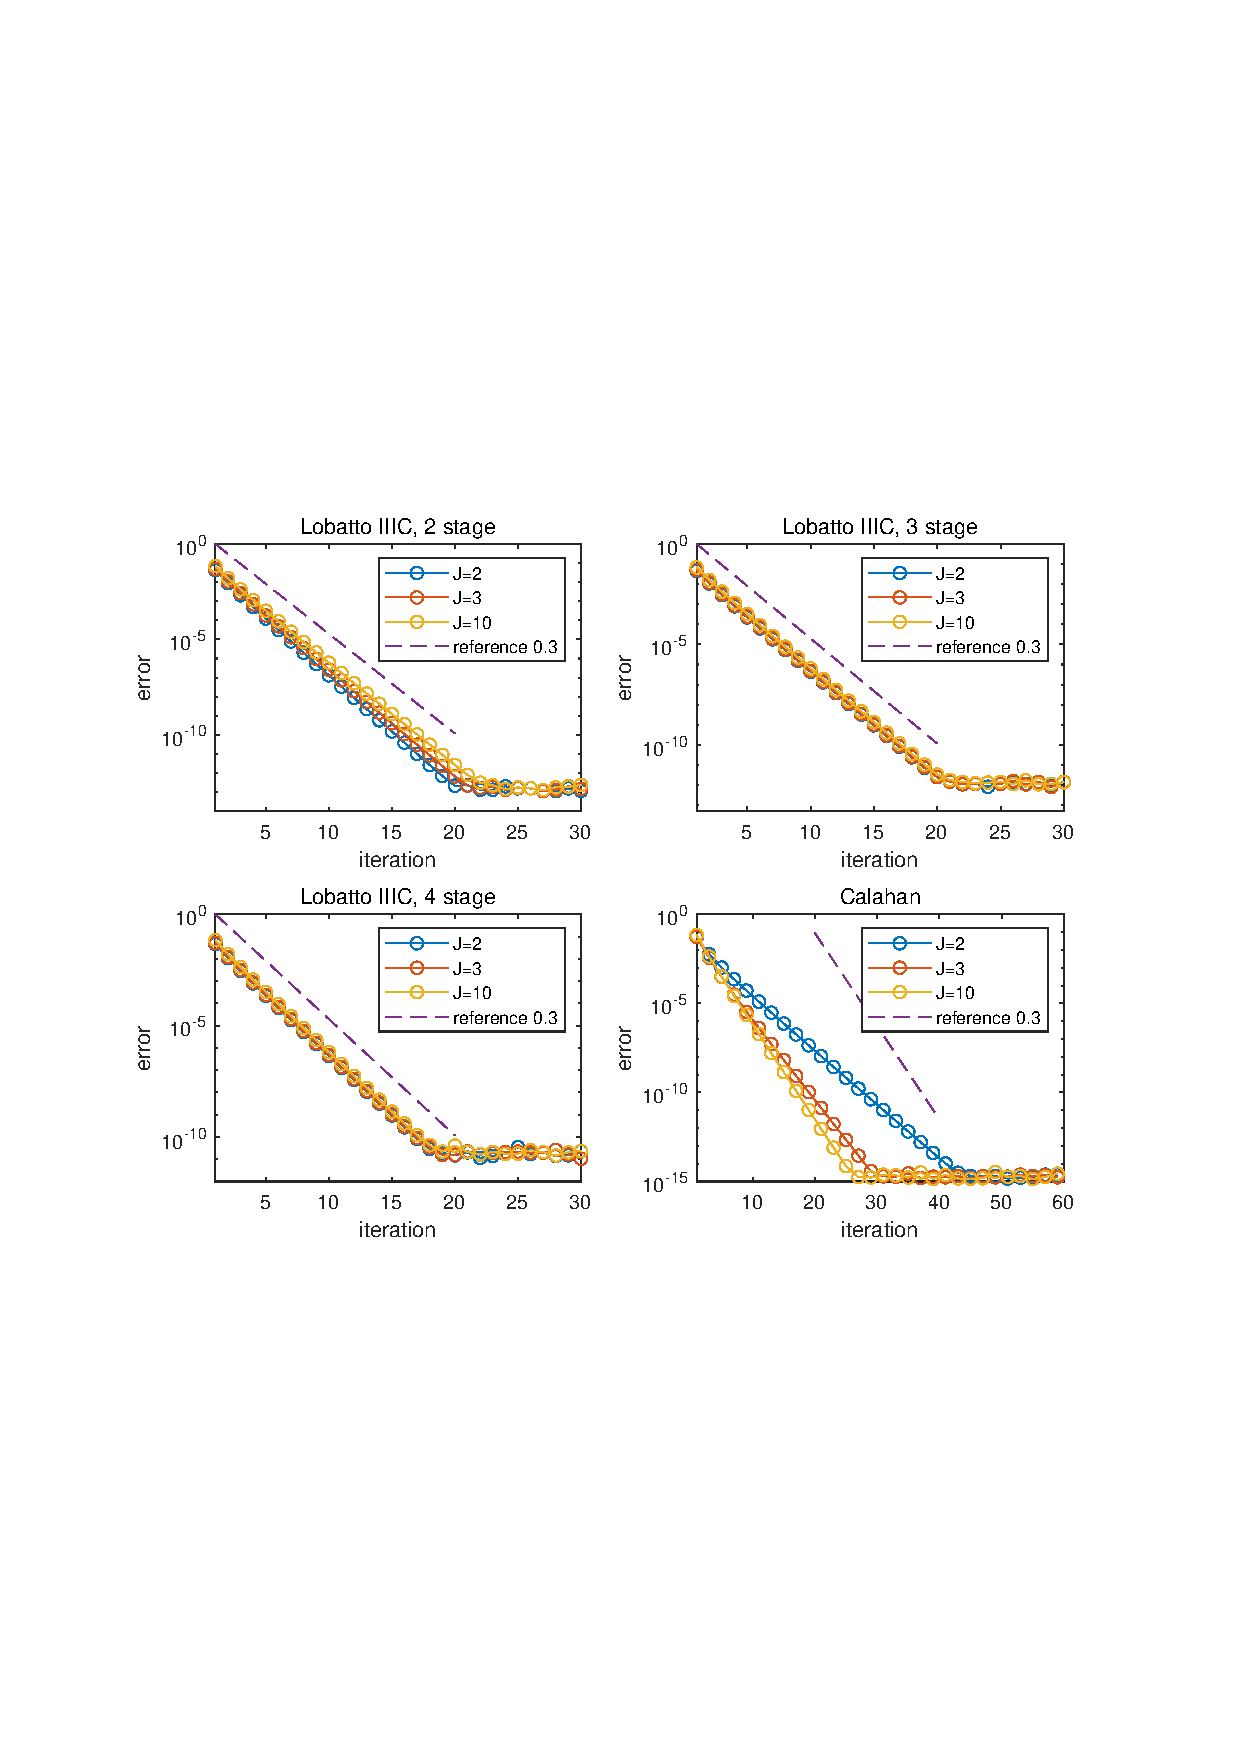
\includegraphics[width=0.9\textwidth]{fig101e.pdf}
   \caption{Example 1 (b): nonsmooth data. Convergence of the parareal algorithm for $2$-, $3$-, $4$-stage Lobatto IIIC methods and Calahan method with fixed fine step size $\Delta t = 1/3000$ and various ratios of coarse step size and fine step size.}
   \label{fig:ex1-b}
\end{figure}

\paragraph{Example 2. Semilinear Parabolic Equations}
In this part, we shall examine the convergence of parareal algorithm for solving the initial-boundary value problem of the semilinear parabolic equations
\begin{equation}\label{eqn:AC2}
\left\{
\begin{aligned}
    \partial_t u   -  \partial_{xx} u &= \frac{1}{\epsilon^2}(u -u ^3)=:f(u ), \quad \text{for all}~~ x\in \Omega,t\in(0,T],\\
    \partial_x u(x,t)&=0, \qquad \qquad  \text{for all}~~ x\in\{0,\pi\},t\in(0,T],\\
    u(x,0)&=u^0(x),\quad\quad \text{for all}~~ x\in \Omega.
\end{aligned}
\right.
\end{equation}
The model \eqref{eqn:AC2}, called Allen--Cahn equation, was originally introduced by Allen and Cahn in \cite{AC} to describe the motion of anti-phase boundaries in crystalline solids. In the context, $u$ represents the concentration of one of the two metallic components of the alloy and
the parameter $\epsilon$ involved in the nonlinear term  represents the width of interface. Recent decades, the Allen--Cahn equation has become one of basic phase-field equations, which has been widely applied to many complicated moving interface problems in materials science and fluid dynamics  \cite{anderson1998diffuse,chen2002phase,yue2004diffuse}.

In our numerical scheme, the coarse propagator  is the semli-implicit backward Euler scheme: for given $u^n$, look for $u^{n+1}$ such that for all $\phi\in H^1(0,\pi)$
$$ (u^{n+1}, \phi) + \Delta T(\partial_{x} u^{n+1},\partial_{x} \phi)= (u^n, \phi) + \Delta T (f(u^n), \phi),$$
which is uniquely solvable and first-order accurate, see e.g. \cite[Theorem 14.7]{Thomee:2006}.
Meanwhile, the fine propagator  is an arbitrary fully implicit high-order single step integrator (such as the Lobatto IIIC schemes or the fully implicit Calahan scheme): for given $u^n$, look for $u^{n+1}$ such that for all $\phi\in H^1(0,\pi)$
\begin{equation}\label{eqn:RK-fully}
\left\{
\begin{aligned}
    (u^{ni},\phi) &= (u^{n-1},\phi) + \Delta t \sum_{j=1}^m a_{ij} \Big(-(\partial_xu^{nj}, \partial_x \phi) +  (f(u^{nj}),\phi) \Big) ~~ \text{for} ~1\le i\le q, \\
    (u^{n},\phi) &= (u^{n-1},\phi) + \Delta t \sum_{i=1}^m b_i \Big(-(\partial_x u^{ni},\partial_x \phi) +  (f(u^{ni}),\phi)\Big),
\end{aligned}
\right.
\end{equation}
where the nonlinear system is uniquely solvable for sufficiently small step size, and we solve it
by use Newton's algorithm. Note that the fine propagator  is fully nonlinear and hence time consuming where the coarse propagator  is a linear scheme, so the application of parareal algorithm is able to significantly improve the efficiency.



\begin{figure} [tbhp]
\centering
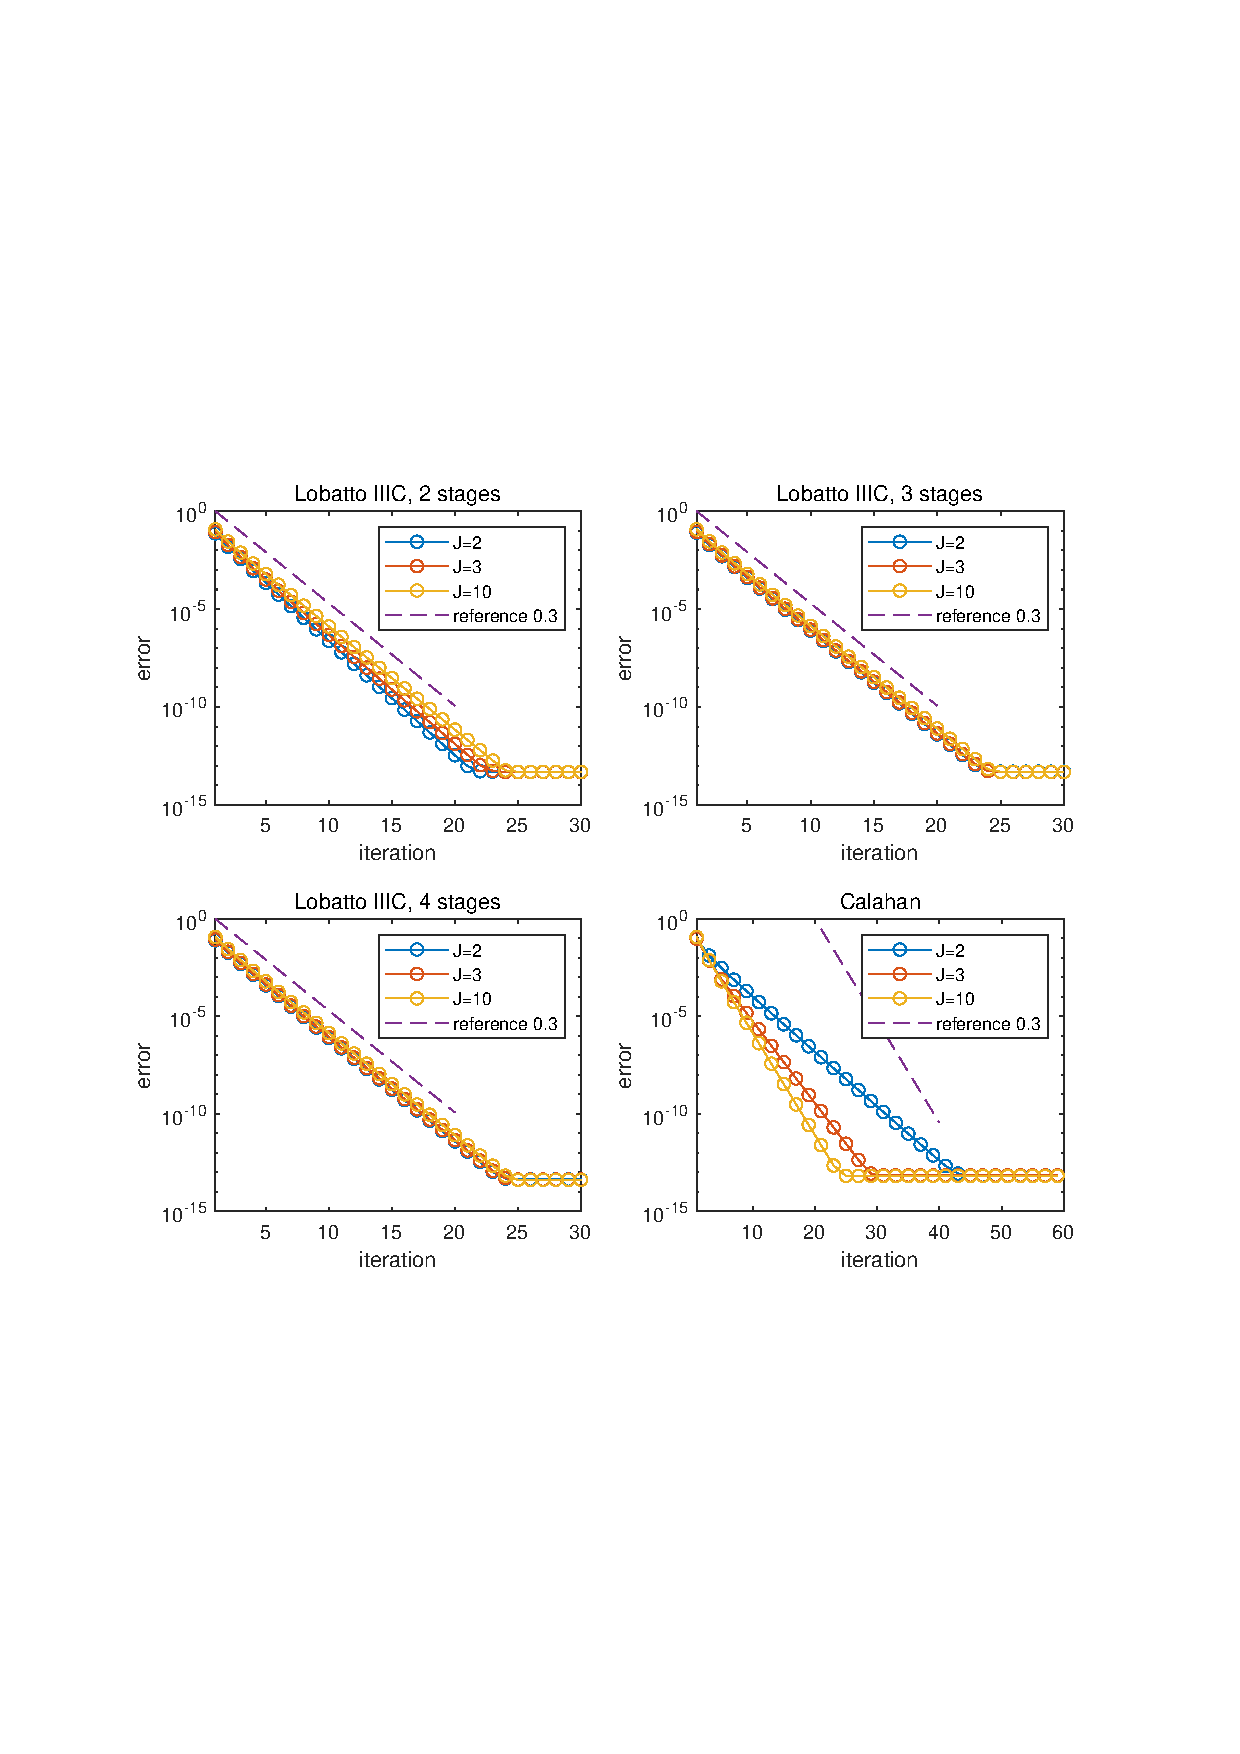
\includegraphics[width=0.9\textwidth]{fig201b.pdf}
   \caption{Example 2. Convergence of the parareal algorithm for $2$-, $3$-, $4$-stage Lobatto IIIC methods and Calahan method with fine step size $\Delta t = 1/600$ and various step ratios $J=2$, $3$, $10$.}
   \label{fig:ex2}
\end{figure}

In Figure \ref{fig:ex2}, we show the convergence of parareal algorithm for $2$-, $3$-, $4$-stage Lobatto IIIC methods and the Calahan method solving
the semilinear parabolic equation \eqref{eqn:AC}
with $\epsilon=1$ and $T=0.1$.
The fine step size is fixed and we examine the convergence for different step ratios.
Similar to the linear problem, for Lobatto IIIC methods,
the numerical experiments clearly show that the parareal iterations converge linearly with convergence factor near $0.3$
for all $J\ge 2$, while for the Calahan method the parareal iterations converge slowly for a small $J$.
The convergence analysis for the nonlinear problem warrants further investigation in our future studies. \vskip10pt

\section{Conclusion and Comments}
In this chapter, we study a parallel-in-time algorithm, named parareal algorithm, to speed up our simulation. We will first start on linear equations. The prove is based on spectrum decomposition. We prove that, for a fixed coarse propagator (Implicit Euler Method), for any single step method fine propagator, as long as the scheme satisfy the given assumptions, we can always find a threshold $J_*$, such that if the mesh ratio $J\geq J_*$, the convergence rate for the iteration is bounded by a given constant about $0.3$. A lot of famous schemes agree with our assumptions. We also tested Allen-Cahn equation and it also works on it. 


%\paragraph{Example 3. 2D Semilinear Parabolic Equations}
%Now we test the convergence of parareal algorithm
%for solving the following Allen--Cahn equation with $\Omega = (0,\pi)^2$.
%\begin{equation}\label{eqn:AC2d}
%\left\{
%\begin{aligned}
%    \partial_t u   -  \Delta u &= \frac{1}{\epsilon^2}(u -u ^3)=:f(u ), \quad \text{for all}~~ x\in \Omega,t\in(0,T],\\
%    \partial_\mathbf{n} u(x, t) &=0, \qquad \qquad  \text{for all}~~ x\in \partial \Omega,t\in(0,T],\\
%    u(x,0)&=u^0(x),\quad\quad \text{for all}~~ x\in \Omega.
%\end{aligned}
%\right.
%\end{equation}
%In our computation, the coarse propagator is the
%semi-implicit backward Euler scheme.
%and the fine propagator is Implicit-Explicit Runge-Kutta (IMEX-RK) Method \cite{lee2020stability}:
%for given $u^n$, look for $u^{n+1}$ such that for all $\phi\in H^1(0,\pi)$
%\begin{equation}\label{eqn:IMRK}
%\left\{
%\begin{aligned}
%    (u^{n1},\phi) &= (u^{n},\phi) - \Delta t (\nabla u^{n1}, \nabla \phi)
%    +\Delta t (f(u^n),\phi), \\
%    (u^{n2},\phi) &= a_{10}(u^{n},\phi) + a_{11}(u^{n1},\phi)
%    - \beta_1 \Delta t (\nabla u^{n2}, \nabla \phi)
%    + \beta_1 \Delta t (f(u^{n1}),\phi), \\
%    (u^{n+1},\phi) &=a_{20}(u^{n},\phi) + a_{21}(u^{n1},\phi) + a_{22}(u^{n2},\phi)
%    - \beta_2 \Delta t (\nabla u^{n+1}, \nabla \phi)
%    + \beta_2 \Delta t (f(u^{n2}),\phi), \\
%\end{aligned}
%\right.
%\end{equation}
%with the coefficients
%$$a_{10}=\frac12,\;a_{11}=\frac12,\;a_{20}=\frac12,\;
%a_{21}=\frac32,\;a_{22}=-1,\;b_1=1,\;b_2=1.$$
%% where the nonlinear system is uniquely solvable for sufficiently small step size, and we solve it
%% by use Newton's algorithm. Note that the fine propagator  is fully nonlinear and hence time consuming where the coarse propagator  is a linear scheme, so the application of parareal algorithm is able to significantly improve the efficiency.
%
%\begin{figure} [tbhp]
%\centering
%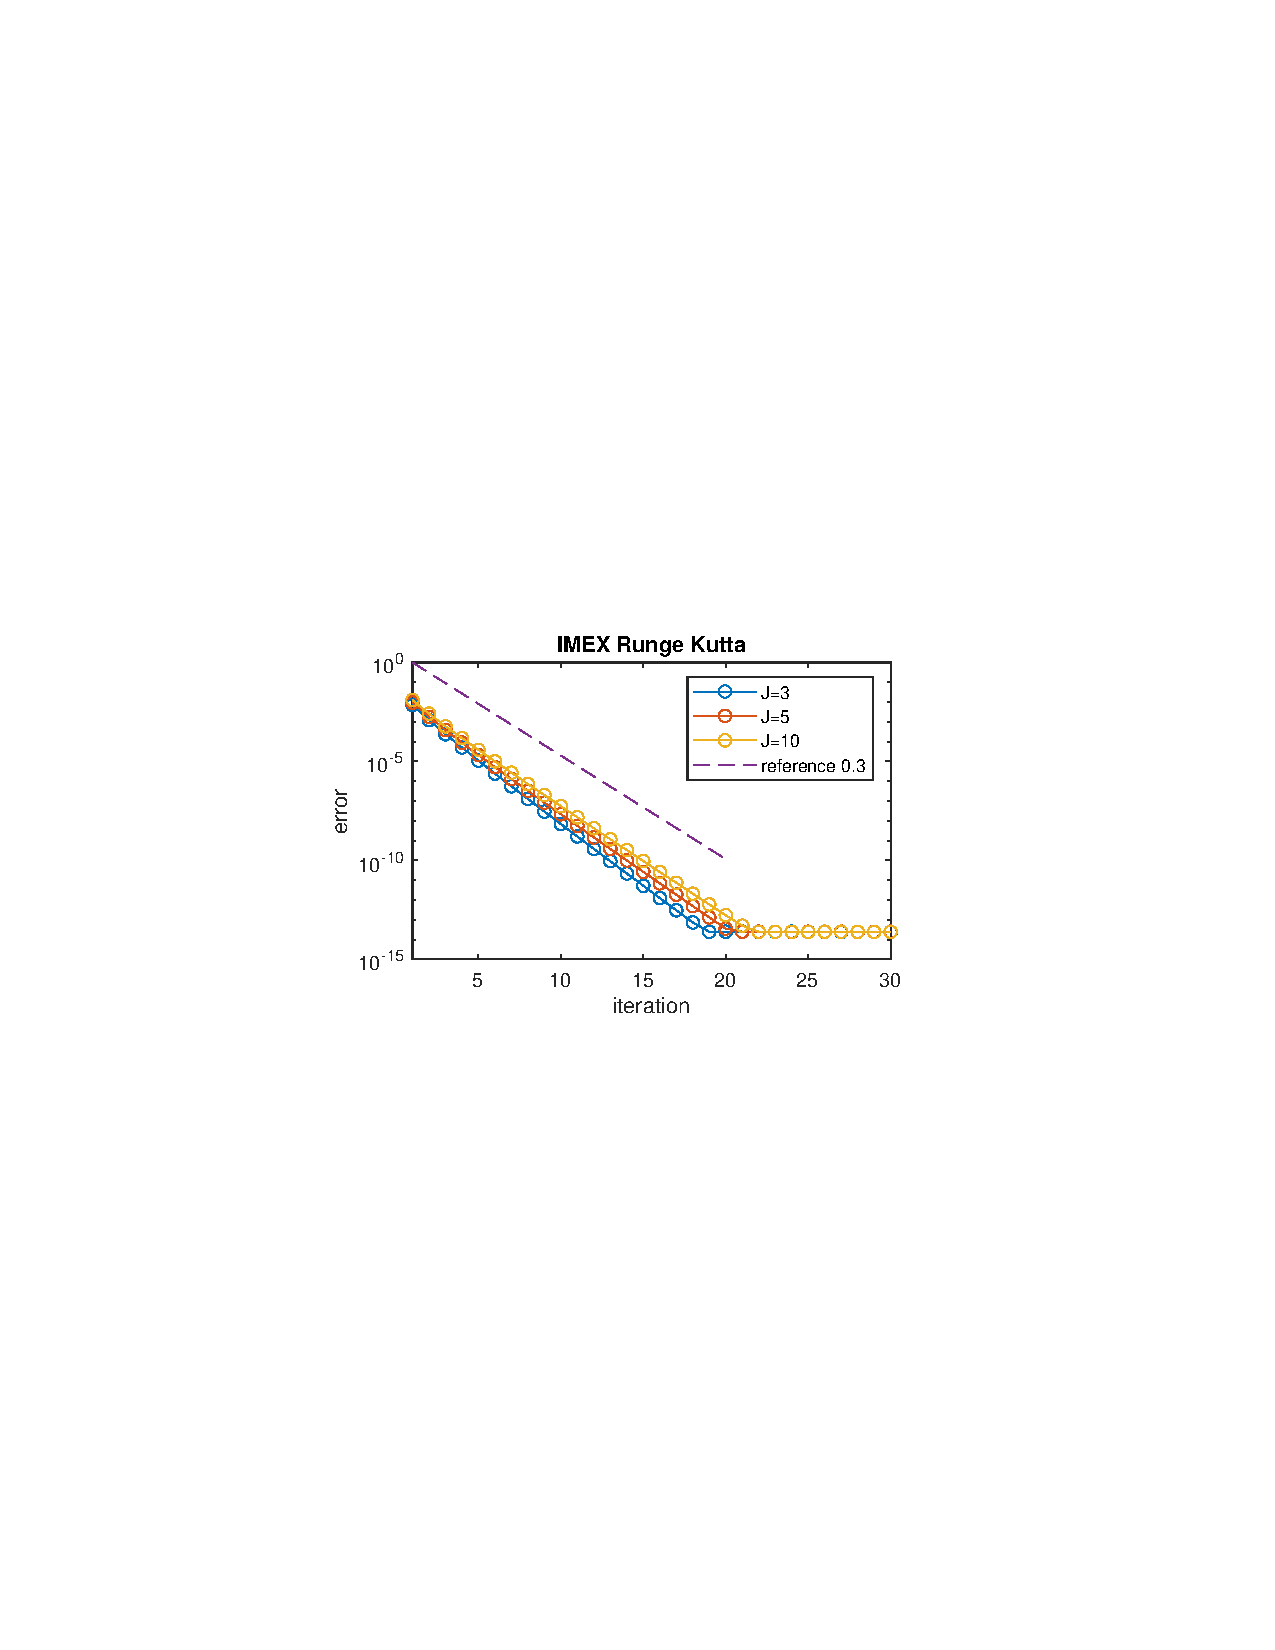
\includegraphics[width=0.45\textwidth]{fig301.pdf}
%   \caption{Example 3. Convergence of the parareal algorithm for
%   IMEX-RK method with fine step size $\Delta t = 1/600$
%   and various step ratios $J=3$, $5$, $10$.}
%   \label{fig:ex3}
%\end{figure}
%In Figure \ref{fig:ex3}, we show the convergence of parareal algorithm
%for IMEX-RK method solving
%the semilinear parabolic equation \eqref{eqn:AC2d}
%with $\epsilon=1$ and $T=1$.
%The fine step size is fixed and we examine the convergence for different step ratios.
%Similar to the linear problem, for IMEX-RK method,
%the numerical experiments clearly show that
%the parareal iterations converge linearly with convergence factor near $0.3$
%for all $J\ge 3$.

% \chapter{Conclusion}



\chapter{Conclusions and Future Work}

This thesis aims to develop efficient single-step methods for solving parabolic problems, particularly in phase-field models, and ensure high accuracy while preserving maximum bound and energy dissipation. 

In the first part of the thesis, we focus on the development and analysis of structure-preserving schemes for solving Allen–Cahn equations, a significant application of parabolic equations. We employ a $k$-th order single-step method in time, linearizing the nonlinear term using multi-step extrapolation. In space, we use a lumped mass finite element method with piecewise $r$-th order polynomials and Gauss–Lobatto quadrature. A cut-off post-processing technique is proposed at each time level to eliminate values violating the maximum bound principle at finite element nodal points. Consequently, the numerical solution adheres to the maximum bound principle at all nodal points, and the optimal error bound $O(\tau^k+h^{r+1})$ is theoretically proven. These time-stepping schemes include algebraically stable collocation-type methods, achieving high order in both space and time. By integrating the cut-off strategy with the scalar auxiliary variable (SAV) technique, we develop energy-stable and maximum bound preserving schemes of arbitrarily high order in time.

In the second part, we start to develop and analyze a class of single-step implicit-explicit schemes for approximately solving linear parabolic equations, achieving long-time stability and arbitrarily high order in time. This approach involves splitting the linear operator into symmetric and skew-symmetric components, which are evaluated implicitly and explicitly respectively using IMEX-RK. For the symmetric part, a diagonally implicit method is employed, while the discretization for the skew-symmetric part is designed to satisfy the stage orders. This method is applicable to semilinear problems, such as phase-field models, and our analysis aligns with existing findings, demonstrating energy stability for certain IMEX-RK schemes. Our results reveal intersections up to at least third order, leading to a scheme that preserves both the original energy decay properties and maximum bound principles.

In the third part of the thesis, we study the parareal algorithm for solving parabolic equations, enabling parallel-in-time computation and significantly accelerating the process. We prove that the parareal method has a robust convergence rate of about $0.3$, provided the ratio $J$ of coarse to fine step size exceeds a certain threshold $J_*$, and the fine propagator meets mild conditions. This convergence holds even with nonsmooth problem data and boundary condition incompatibilities. Qualified methods include all absolutely stable single-step methods with a stability function satisfying $\lvert r(-\infty) \rvert < 1$, allowing the fine propagator to be of arbitrarily high order. We also examine popular high-order single-step methods, such as the two-, three-, and four-stage Lobatto IIIC methods, confirming that their corresponding parareal algorithms converge linearly with a factor of $0.31$ and a threshold $J_* = 2$. At the end of each chapter, we present numerical results that support the theoretical findings and inspire future investigations.

Next we list several perspectives for the future research:
\begin{itemize}
    \item[1.] Cut-off postprocessing can naturally ensure maximum bound preservation and maintain energy decay when the function is continuous in space or uses piecewise linear FEM. However, for higher-order finite elements, like $P^2(I)$ for $I \subset \mathbb{R}^1$, a simple cut-off on $u$ may increase $|\nabla u|$, causing our analysis to fail. Thus, for both cut-off RK-SAV, which preserves maximum bounds and modified energy decay, and cut-off IMEX-RK, which preserves maximum bounds and original energy decay, we achieve at most second-order spatial accuracy in fully discretized problems. We need to explore alternative methods, such as enhanced cut-off or other postprocessing techniques, to achieve higher-order spatial convergence, requiring further study.
    \item[2.] In the proof of long-time error estimate for linear implicit-explicit Runge-Kutta methods, we assume $0 < \sigma(\lambda) < 1$, which is equivalent to $|\sigma| < 1$ and $\sigma > 0$. We require $\sigma > 0$ to ensure the inverse operator and norms are well-posed. Although this condition seems redundant, the proof fails without it. We hope to address this issue in the future.
    \item[3.] We use the undetermined coefficients method to explore implicit-explicit Runge-Kutta schemes. Although there are more degrees of freedom than equations, we have not shown that these schemes can achieve arbitrarily high order. Unlike the usual Runge-Kutta method, where high-order schemes can be systematically built, this approach does not work for implicit-explicit Runge-Kutta. Developing an algorithm to construct high-order implicit-explicit Runge-Kutta schemes, rather than searching for them, could be beneficial.
    \item[4.] When applying IMEX-RK schemes to solve gradient flow models, preserving the energy dissipation property is crucial. Unfortunately, this requires strict conditions, including the positive-definiteness of coefficient matrices, which are more complex than algebraic stage-order conditions. Consequently, our strategy fails to ensure the energy dissipation property for high-order schemes. While we have not ruled out the possibility of IMEX-RK achieving higher order for original energy decay, we have only found first, second, and third-order results. Discovering fourth or higher-order schemes would be both important and interesting.
    \item[5.] We established the robust convergence rate for the parareal method using a single-step approach. Extending this work to multi-step methods, such as BDF, is intriguing. Developing the coarse propagator carefully is crucial to prevent algorithm instability. Understanding the conditions for convergence and creating a suitable coarse propagator is essential for applying the parareal method to a wider range of scenarios.
    \item[6.] Although we have only proven robust convergence for the parareal method on linear equations, numerical experiments indicate it also performs well on nonlinear models, such as the Allen-Cahn equations, with similar convergence behavior. Various coarse propagators can be used, each behaving differently, and some achieving excellent convergence. Developing the theory and analysis for the parareal method on semilinear equations with nonsmooth data is needed. 
\end{itemize}




\chapter*{References}

\printbibliography[heading = none]
% \printbibliography


\end{document}

